\documentclass{article}
\usepackage[utf8]{inputenc}
\usepackage{graphicx}
\usepackage[english]{babel}
\usepackage{ragged2e}
\usepackage{blindtext}
\usepackage{listings}
\usepackage[a4paper, total={6in, 9in}]{geometry}
\usepackage{xcolor}
\usepackage{graphicx} %package to manage images
\graphicspath{ {./photo/} }
\usepackage{multicol}

%New colors defined below
\definecolor{codegreen}{rgb}{0,0.6,0}
\definecolor{codegray}{rgb}{0.5,0.5,0.5}
\definecolor{codepurple}{rgb}{0.58,0,0.82}
\definecolor{backcolour}{rgb}{0.95,0.95,0.92}

%Code listing style named "mystyle"
\lstdefinestyle{mystyle}{
  backgroundcolor=\color{backcolour}, commentstyle=\color{codegreen},
  keywordstyle=\color{magenta},
  numberstyle=\tiny\color{codegray},
  stringstyle=\color{codepurple},
  basicstyle=\ttfamily\footnotesize,
  breakatwhitespace=false,         
  breaklines=true,                 
  captionpos=b,                    
  keepspaces=true,                 
  numbers=left,                    
  numbersep=5pt,                  
  showspaces=false,                
  showstringspaces=false,
  showtabs=false,                  
  tabsize=2
}

\begin{document}

\pagenumbering{Italic}

% -------------------Cover Page--------------------------%

\begin{titlepage}
    \begin{center}
        \textbf {\Huge {University of Rajshahi}} \\
        \hfill \break
    \end{center} 
    \begin{figure}[h]
        \centering
        
\includegraphics[width=0.4\textwidth]{ru.jpg}
    \end{figure}
    \begin{center}
        \hfill \break
        \hfill \break
        \textbf{\Huge {Assignments of DIP Lab}} \\
        \hfill \break
        \LARGE {Course Name: Digital Image Processing Lab} \\
        \LARGE {Course Code: CSE-4182} \\
        \Large {Date: \today} \\
        \hfill \break
        \hfill \break
        \begin{multicols}{2}
        \raggedright
        \Large {\textbf{Prepared by}} \\
        \large {Name: Md. Meem Mursalin Chowdhury} \\ 
        \large {ID: 1810276103} \\
        \large {Year: 4th, Semester: Odd} \\
        \large {Session: 2017-18} \\
        \LARGE {\textbf{Submitted to}} \\
        \large {Md. Khademul Islam Molla, Professor} \\
        \large {MD. Rokanujjaman, Professor} \\
        \large {Sangeeta Biswas, Associate Professor}
        \hfill \break
        \end{multicols}
        \hfill \break
        \hfill \break
        \LARGE {Dept. of Computer Science and Engineering,\\ University of Rajshahi} \\
    \end{center}
\end{titlepage}

%-----------------------Abstract page-------------------------%
{
    \centering
    \section*{Abstract}
    \justifying {Digital Image Processing or DIP is a very well-known term to most of the people. It refers to the processing of different images. This processing is done images on basis of the need and demand. In this lab all the images are processed using python3 and the grayscale images or 2D images are considered.\\}    
    \pagenumbering{roman}
    \clearpage
}

%---------------------Table of Contents-----------------------%

\tableofcontents
% \pagebreak
\clearpage

%-----------------------Assignment-1--------------------------%
{
    \section{Assignment-1}
    \pagenumbering{arabic}
    \setcounter{page}{1}
    \subsection{Introduction}
    \textbf {Problem: }
    Plot histogram of the grayscale, red channel, green channel, blue channel and binary image of an RGB image. You may take help from the following link:\\
    \https{https://docs.opencv.org/4.x/d1/db7/tutorial\_py\_histogram\_begins.html}\\
    
    When you upload any assignments, please follow the following rules:\\
    1. If there are multiple files, put them in a zip file, and name that zip by your StudentID, not by name.\\
    2. For a single file, name that file by your StudentID, not by name.\\
    For Assignment1, upload one figure with rgb, red, green, blue, grayscale and binary  images and one figure with histograms.\\
    \\
    \textbf{Solution: }
    Here we have to plot histogram of the grayscale, red channel, green channel, blue channel and binary image of an RGB image. To do this, at first we have to read/load the RGB image. Then we have to separate the RGB image into 3 channels such as red, green and blue. After that we have to again convert the RGB image to grayscale image. At last, all the results will have to plot as histogram. For doing this, the required program is given below.
    \\
    
    \subsection{Required Software}
    For completing this task, we have to install open-cv and matplotlib. In our program, we have to import the open-cv(cv2) and matplotlib.pyplot as plt. We can install this two using pip3. For different operations both open-cv(cv2) and matplotlib will have to be used - specially matplotlib for plotting and saving image. 
    \\
    
    \subsection{Procedure}
    \textbf{Step-1:}
    Install matplotlib, open-cv libraries.\\
    \textbf{Step-2:}
    Import them in our program. (matplotlib.pyplot as plt, cv2 as cv)\\
    \textbf{Step-3:}
    Read the RGB image.\\
    \textbf{Step-4:}
    Separate the RGB image in 3 different channels - red, green, blue and save them in different variables.\\
    \textbf{Step-5:}
    Convert the RGB image in grayscale using cv.cvtColor() function and binary using cv.threshold() function and save them.\\
    \textbf{Step-6:}
    Create and save histogram of required task using cv.calcHist() function and save them.\\
    \textbf{Step-7:}
    Plot all the required images and save them as required in the question.\\
    
    \subsection{Code}
    \lstset{style=mystyle}
    \begin{lstlisting}[language=Python, caption=Code for histogram and picture of different channels]
    import matplotlib.pyplot as plt
    import cv2 as cv
    
    def main():
    	img_path = './trees_in_water_3.jpg'
    	print(img_path)
    	
    	rgb = plt.imread(img_path)
    
    	red = rgb[:, :, 0]
    	green = rgb[:, :, 1]
    	blue = rgb[:, :, 2]
    
    	histRed = cv.calcHist([rgb],[0],None,[256],[0,256])
    	histGreen = cv.calcHist([rgb],[1],None,[256],[0,256])
    	histBlue = cv.calcHist([rgb],[2],None,[256],[0,256])
    
    	grayscale = cv.cvtColor(rgb, cv.COLOR_RGB2GRAY)
    	histGrayscale = cv.calcHist([grayscale],[0],None,[256],[0,256])
    
    	_, binary = cv.threshold(grayscale, 127, 255, cv.THRESH_BINARY)
    	histBinary = cv.calcHist([binary],[0],None,[256],[0,256])
    
    	img_set = [rgb, red, green, blue, grayscale, binary]
    	hist_set = [rgb, histRed, histGreen, histBlue, histGrayscale, histBinary]
    	title_set = ['RGB', 'Red', 'Green', 'Blue', 'Grayscale', 'Binary']
    	
    	plt.figure(figsize = (20, 20))
    	for i in range(6):
    		plt.subplot(2, 3,  i + 1)
    		plt.title(title_set[i])
    		ch = len(img_set[i].shape)
    		if (ch == 3):
    			plt.imshow(img_set[i])
    		elif (i == 1 or i == 2 or i == 3):
    			plt.imshow(img_set[i], cmap = title_set[i] + 's')
    		else: 
    			plt.imshow(img_set[i], cmap = 'gray')			
    	plt.savefig('fig-1.jpg')
    	plt.show()
    	
    	plt.figure(figsize = (15, 15))
    	for i in range(6):
    		plt.subplot(2, 3,  i + 1)
    		plt.title(title_set[i])
    		if (i == 0):
    			plt.plot(histRed, 'r')
    			plt.plot(histGreen, 'g')
    			plt.plot(histBlue, 'b')
    		else:
    			plt.plot(hist_set[i])
    	plt.savefig('fig-2.jpg')
    	plt.show()
    	
    
    if __name__ == '__main__':
    	main()

    \end{lstlisting}
    \\
    \subsection{Result & Discussion}{
        Here, as at first, we read/load the RGB image and then separate it in 3 different channels. Then we convert the RGB image in grayscale and binary. After that the histogram of all the save image is obtained and the required images of histogram and image channels and conversion are saved and plotted as follows. So, the task is completed.
        
        \begin{figure}[htp]
            \centering
            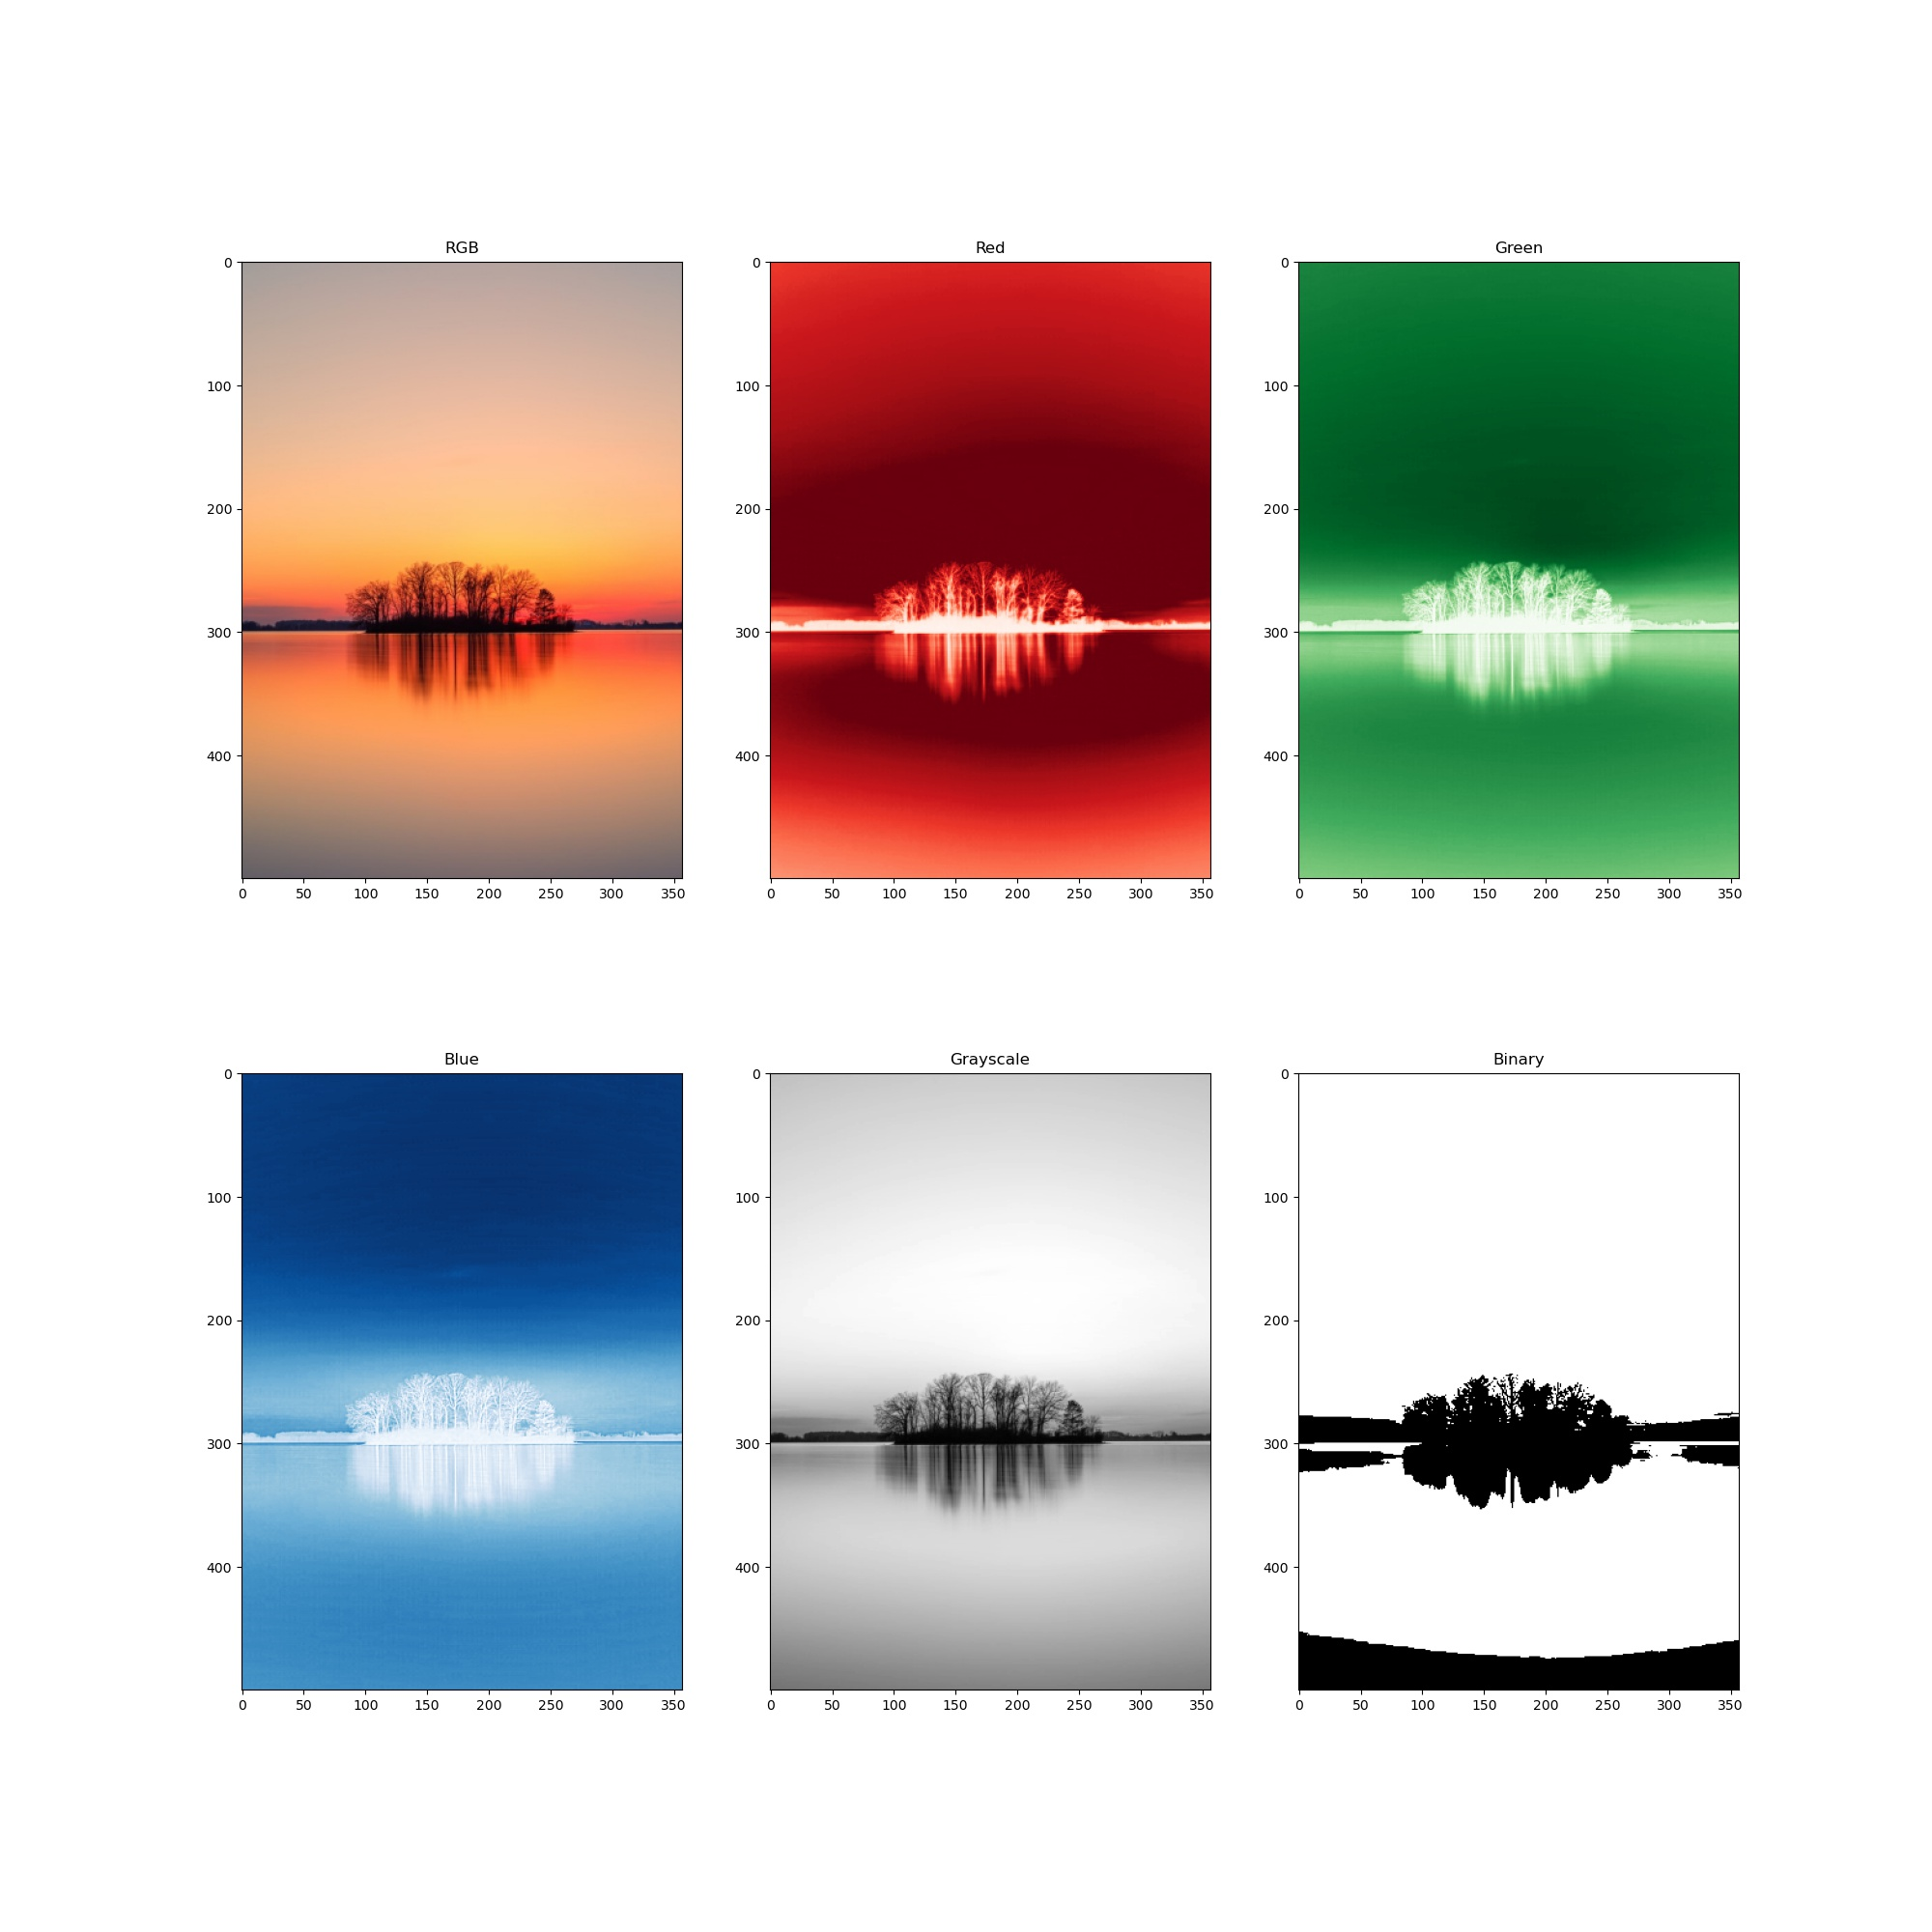
\includegraphics[width=.70\textwidth]{Assignment-1/fig-1.jpg}
            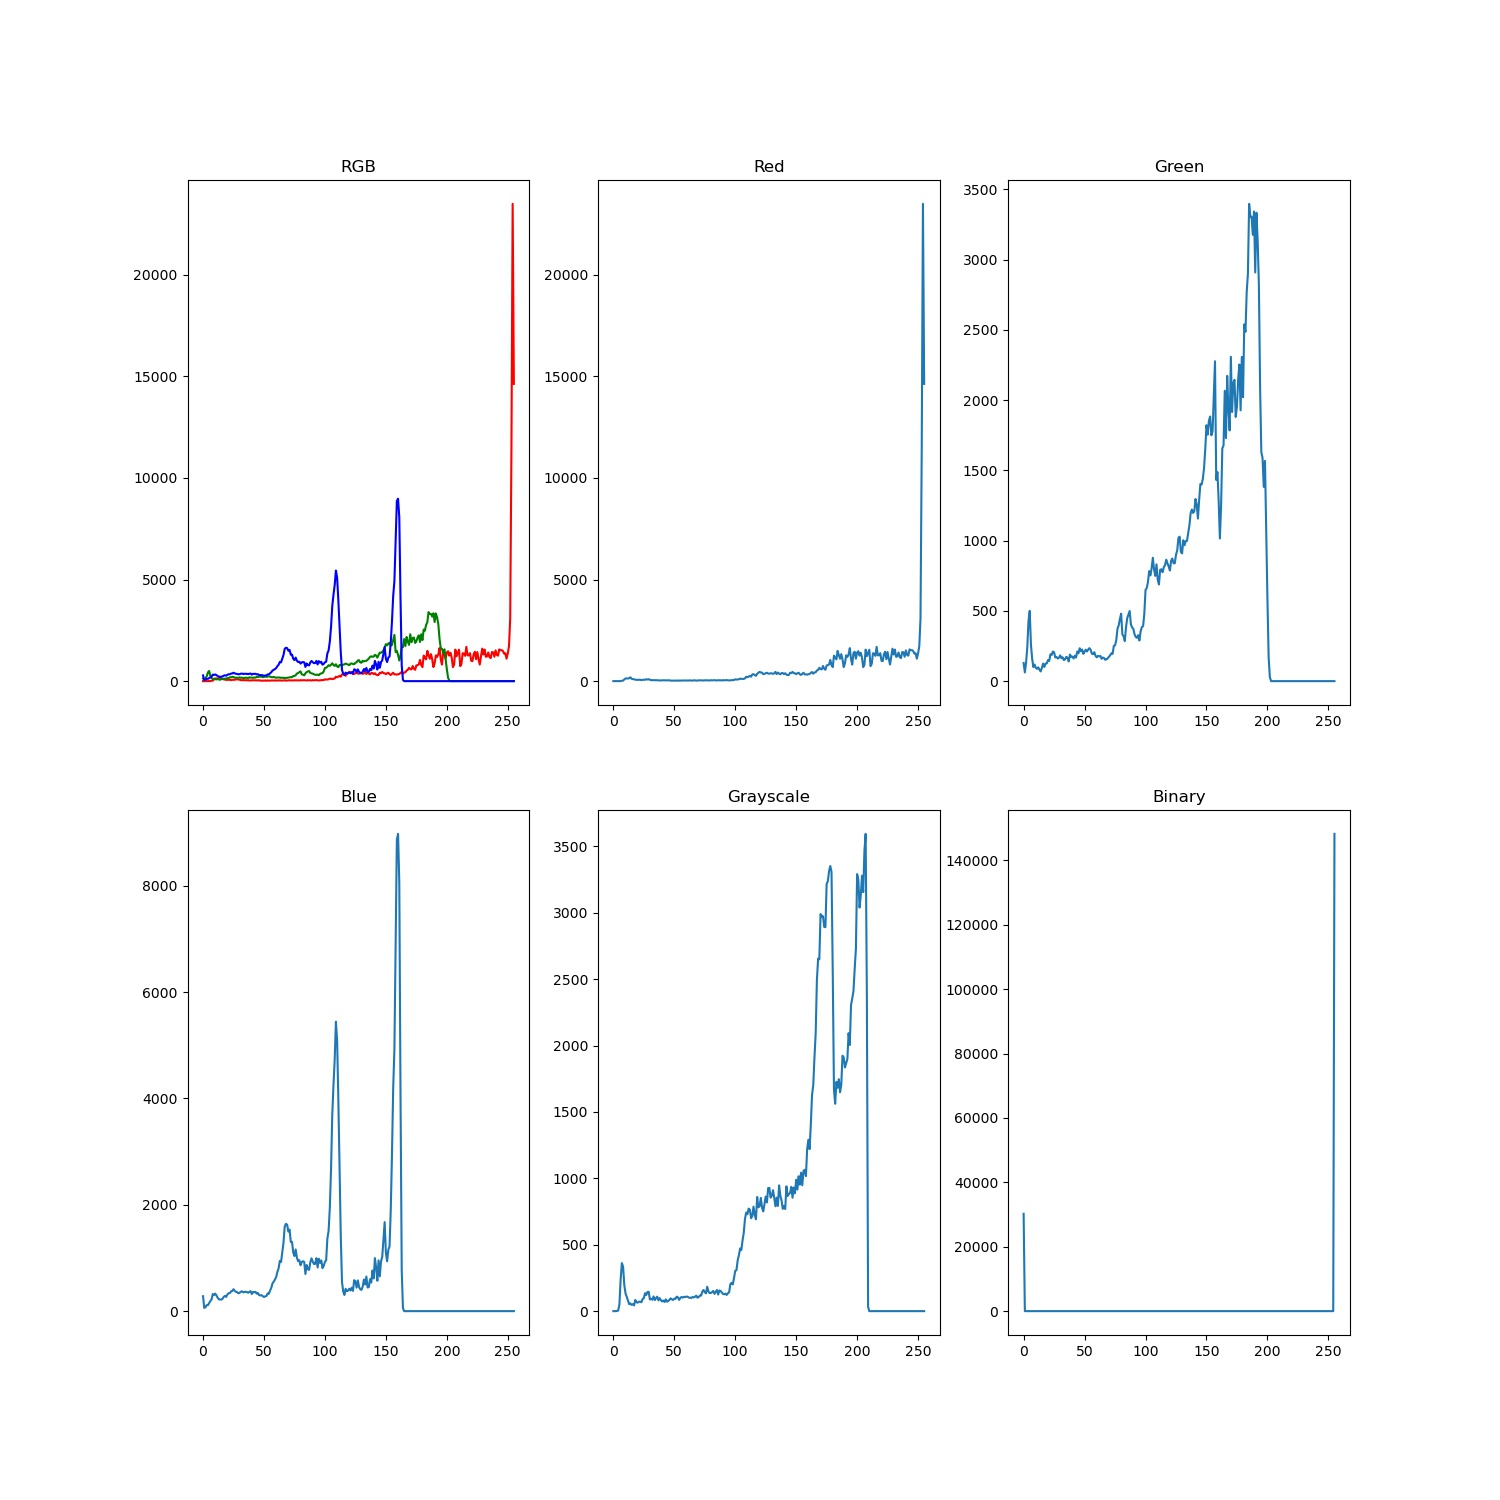
\includegraphics[width=.70\textwidth]{Assignment-1/fig-2.jpg}
            \caption{Input image and images of different channels and grayscale and binary image, Histogram of all previous image}
        \end{figure}
    }
}
% \pagebreak
\clearpage

%-----------------------Assignment-2--------------------------%
{
    \section{Assignment-2}
    \subsection{Introduction}
    \textbf {Problem: }
    Perform point processing on a 2D image:\\
    Let 'r' is the old intensity of a pixel and 's' is the new intensity. Let
    'c' and 'p' are two positive constants. You can assume any value for 'c
    and 'p'. For 'epsilon' choose very small value, such as 0.0000001. 'T1'
    and 'T2' are two thresholds. You can assume any value in the range 0 -
    255.\\
    Check what happens for the following transformations:\\
    1. $s = 100$, if $r >= T1$ and $r <= T2$; otherwise $s = 10$\\
    2. $s = 100$, if $r >= T1$ and $r <= T2$; otherwise $s = r$\\
    3. $s = c*log(1 + r)$\\
    4. $s = c ( r + epsilon ) ^ p$\\
    \\
    \textbf{Solution: }
    Here, basically we have to do point processing. For the first two tasks, we have some threshold value on basis of which we have to do some operation with fixed values. Again, for task-3 and task-4 we have to directly apply some operation of some fixed values. To do this, the following program is used.
    \\
    
    \subsection{Required Software}
    For completing this task, we have to install open-cv, matplotlib and numpy. In our program, we have to import the open-cv(cv2), matplotlib.pyplot as plt and numpy as np. We can install this three libraries using pip3. For different operations open-cv(cv2), numpy and matplotlib will have to be used - specially matplotlib for plotting and saving image. 
    \\
    
    \subsection{Procedure}
    \textbf{Step-1:}
    Install matplotlib, open-cv, numpy libraries.\\
    \textbf{Step-2:}
    Import them in our program. (matplotlib.pyplot as plt, cv2 as cv, numpy as np)\\
    \textbf{Step-3:}
    Read the RGB image.\\
    \textbf{Step-4:}
    Perform the point processing according to the given values. Use numpy for task-3 and task-4 specially. Save the output.\\
    \textbf{Step-5:}
    Plot all the required images and save them as required in the question.\\
    
    \subsection{Code}
    \lstset{style=mystyle}
    \begin{lstlisting}[language=Python, caption=Code for point processing and thresholding]
    import matplotlib.pyplot as plt
    import cv2 as cv
    import numpy as np
    
    def main():
        img_path = 'trees_in_water_3.jpg'
        print(img_path)
        rgb = plt.imread(img_path)
        print(rgb.shape)
    
        T1 = 80
        T2 = 150
        c = 10
        p = 2
        epsilon = 1e-6
    
        grayscale = cv.cvtColor(rgb, cv.COLOR_RGB2GRAY)
        r, c = grayscale.shape
        processed_img1 = 10 * np.ones((r, c), dtype = np.uint8)
        for x in range(r):
            for y in range(c):
                if (grayscale[x][y] > T1 and grayscale[x][y] < T2):
                    processed_img1[x][y] = 100
                    
        processed_img2 = [row[:] for row in grayscale]
        for x in range(r):
            for y in range(c):
                if (processed_img2[x][y] > T1 and processed_img2[x][y] < T2):
                    processed_img2[x][y] = 100
    
        processed_img3 = c * np.log(1 + grayscale)
        # processed_img3 = grayscale
        # for x in range(r):
        #     for y in range(c):
        #         processed_img3[x][y] = c*np.log(1+processed_img3[x][y])
    
        processed_img4 = c * ((epsilon + grayscale) ** p)
    
        img_set = [rgb, grayscale, processed_img1, processed_img2, processed_img3, processed_img4]
        title_set = ['RGB', 'Grayscale', 'Processed Image 1', 'Processed Image 2', 'Processed Image 3', 'Processed Image 4']
        plot_img(img_set, title_set)
    
    def plot_img(img_set, title_set):
        plt.figure(figsize = (20, 20))
        n = len(img_set)    
        for i in range(n):
            plt.subplot(2, 3, i+1)
            plt.title(title_set[i])
            if (i == 0):
                plt.imshow(img_set[i])
            else:
                plt.imshow(img_set[i], cmap = 'gray')
        plt.savefig('fig-1.jpg')    
        plt.show()
    
    if __name__ == '__main__':
        main()

    \end{lstlisting}
    \\
    \subsection{Result & Discussion}{
        Here, as at first, we read/load the RGB image and then perform the different operation accordingly. Then we save the image and plot them as follows. So, the task is completed.
        
        \begin{figure}[htp]
            \centering
            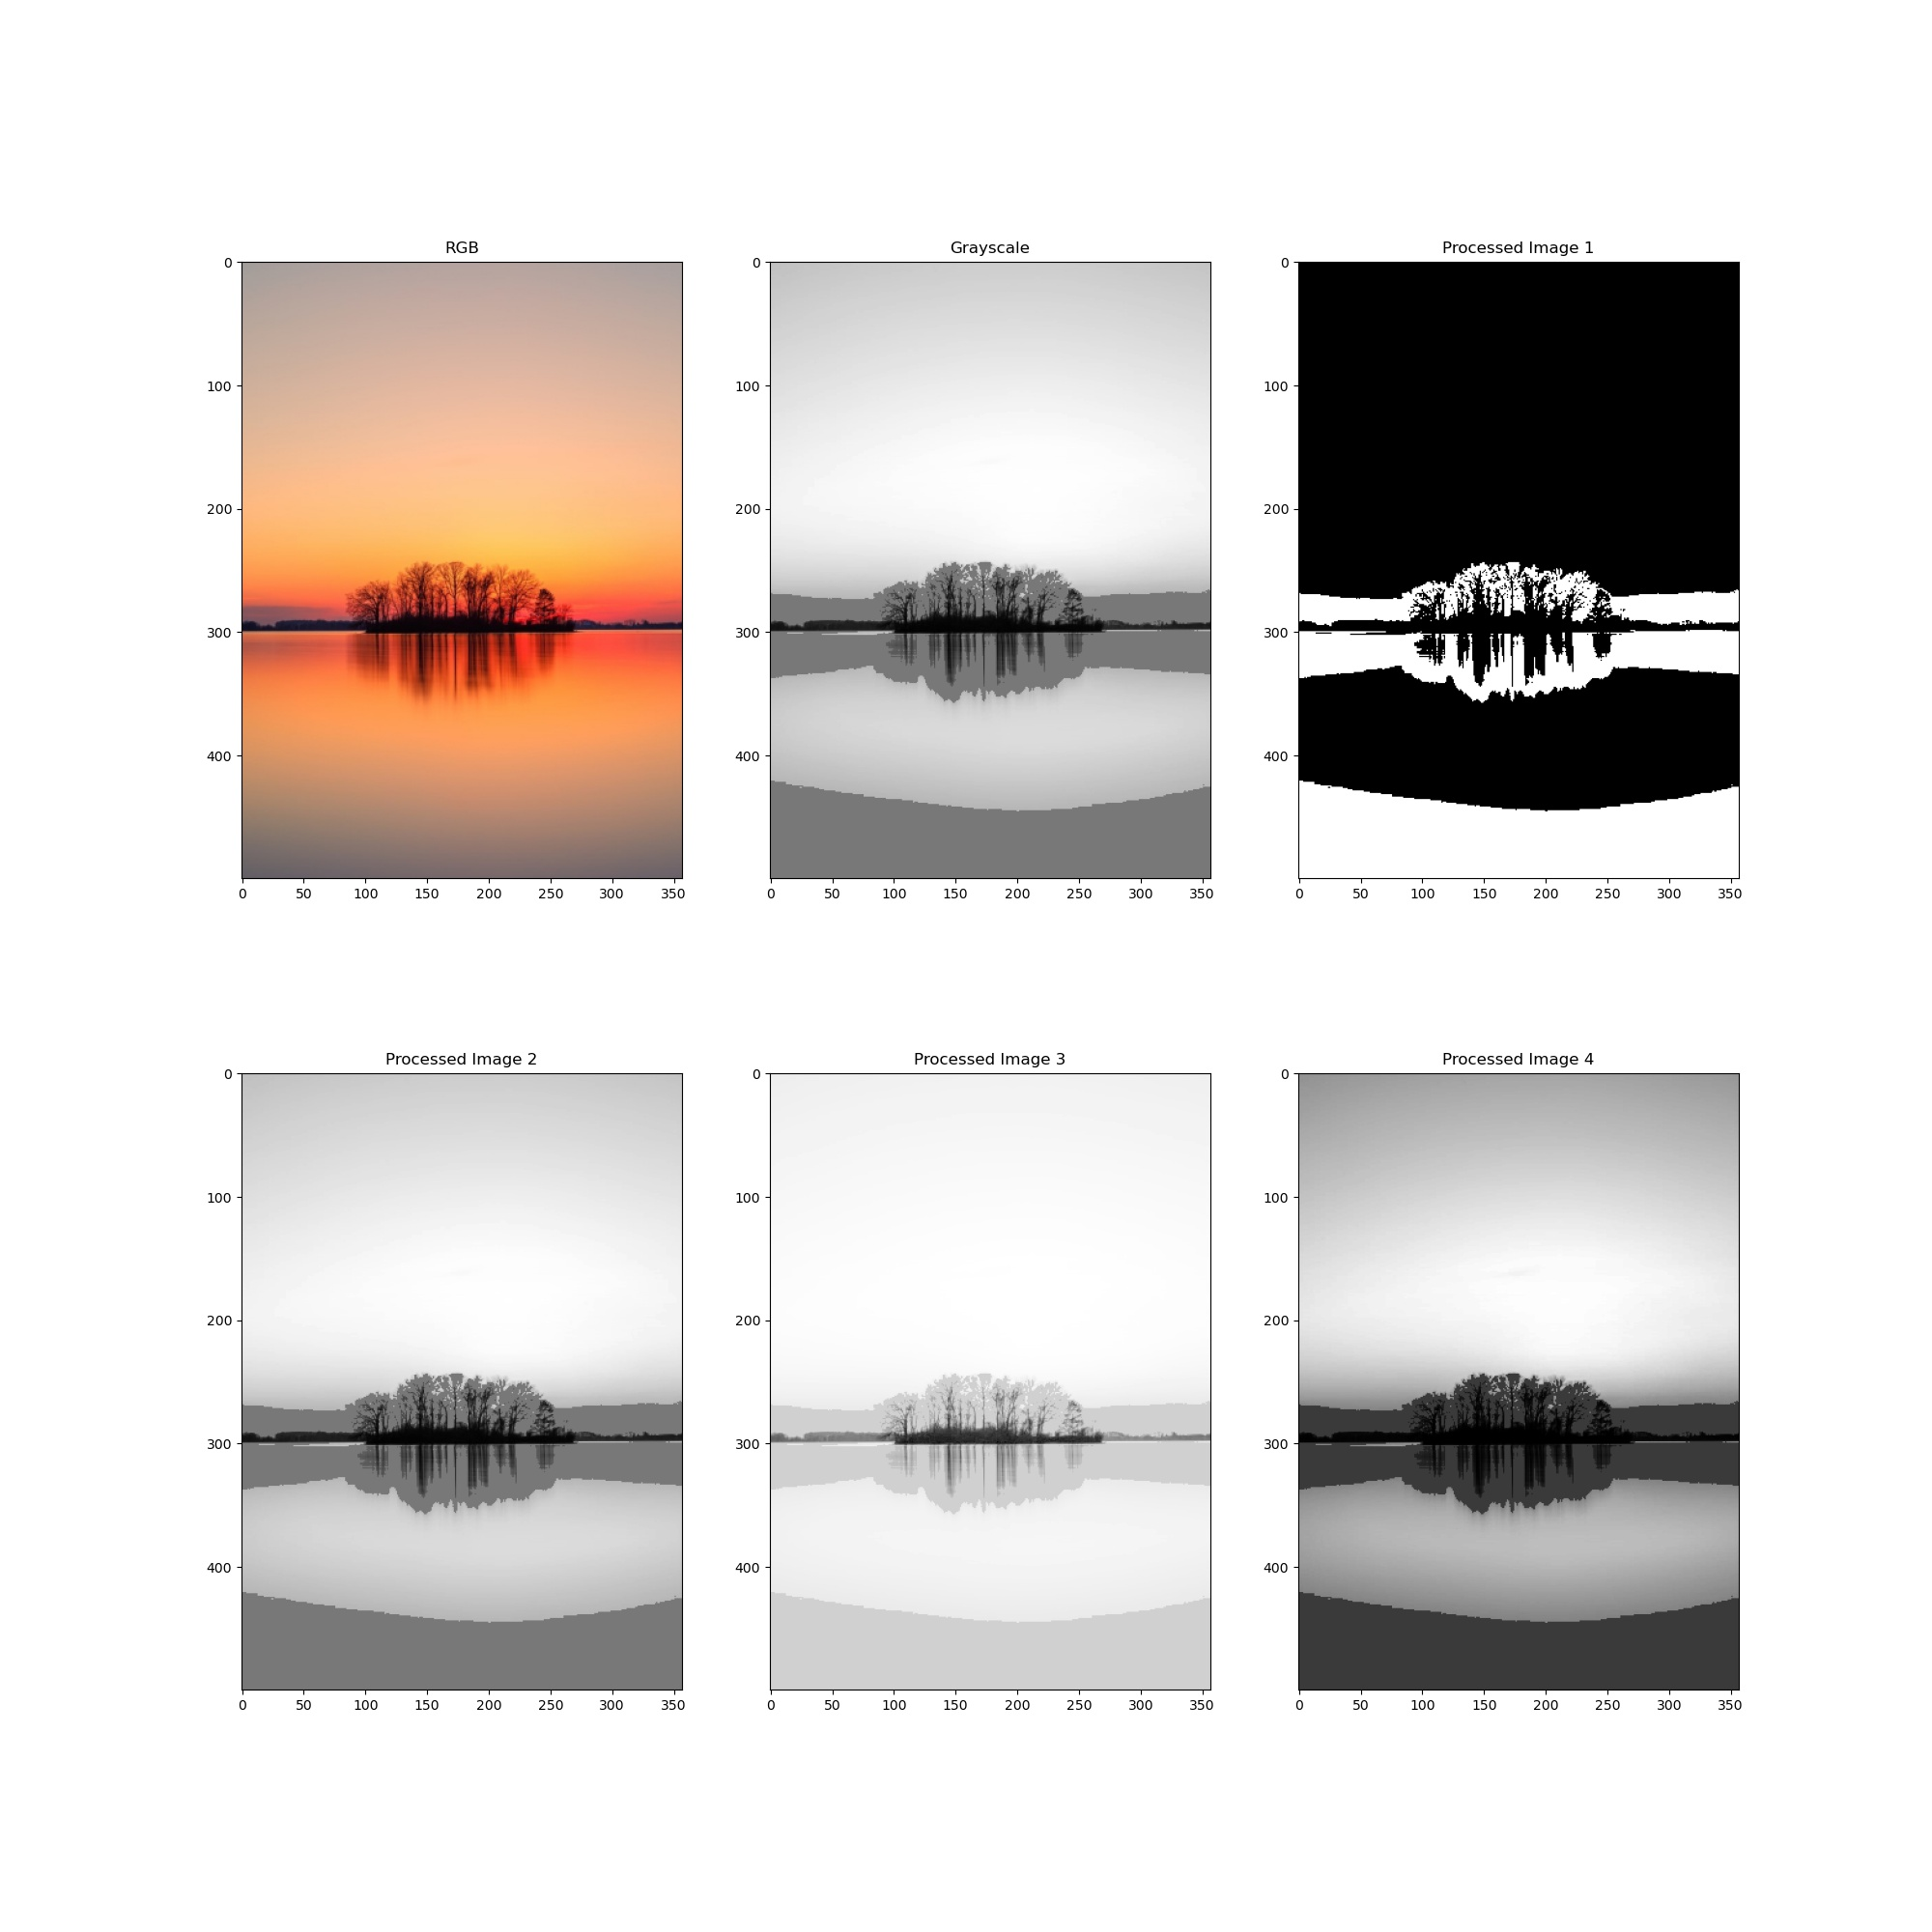
\includegraphics[width=1.0\textwidth]{Assignment-2/fig-1.jpg}
            \caption{Input image and output images of point processing}
        \end{figure}
    }
}
% \pagebreak
\clearpage

%-----------------------Assignment-3--------------------------%
{
    \section{Assignment-3}
    \subsection{Introduction}
    \textbf {Problem: }
    Show the effect of 6 different kinds of kernels on a 2D image.
    Conditions:
    Kernels of each student  need to be  different from kernels of other students and kernels used in provided code.\\
    \\
    \textbf{Solution: }
    Here, we have to do convolution operation on a grayscale image whiche basically neighbourhood processing. We can use the built-in function here. So, we have to just load the image and perform the operation using the built-in function and save the output and show ti. To do this, the following program is used.
    \\
    
    \subsection{Required Software}
    For completing this task, we have to install open-cv, matplotlib and numpy. In our program, we have to import the open-cv(cv2), matplotlib.pyplot as plt and numpy as np. We can install this three libraries using pip3. For different operations open-cv(cv2), numpy and matplotlib will have to be used - specially matplotlib for plotting and saving image. 
    \\
    
    \subsection{Procedure}
    \textbf{Step-1:}
    Install matplotlib, open-cv, numpy libraries.\\
    \textbf{Step-2:}
    Import them in our program. (matplotlib.pyplot as plt, cv2 as cv, numpy as np)\\
    \textbf{Step-3:}
    Read the RGB image and convert it to grayscale using cv.cvtColor() function.\\
    \textbf{Step-4:}
    Perform the filter operation (neighbourhood processing) for different filters. Use numpy for creating our filters and cv.filter2D() function for performing filter operation. Save the output.\\
    \textbf{Step-5:}
    Plot all the required images and save them as required in the question.\\
    
    \subsection{Code}
    \lstset{style=mystyle}
    \begin{lstlisting}[language=Python, caption=Code for image filtering based on different filters]
    import matplotlib.pyplot as plt
    import cv2 as cv
    import numpy as np
    
    def main():
        img_path = './table.jpg'
        rgb = plt.imread(img_path)
        print(rgb.shape)
    
        grayscale = cv.cvtColor(rgb, cv.COLOR_RGB2GRAY)
        print(grayscale.shape)
    
        horizontalKernel = np.array([[3, 10, 3],[0, 0, 0], [-3, -10, -3]])
        verticalKernel = np.array([[3, 0, -3],[10, 0, -10], [3, 0, -3]])
        sharpenKernel = np.array([[0, -1, 0],[-1, 5, -1], [0, -1, 0]])
        identityKernel = np.array([[0, 0, 0],[0, 1, 0], [0, 0, 0]])
        boxBlurKernel = 1/9 * np.array([[1, 1, 1],[1, 1, 1],[1, 1, 1]])
        gaussianBlurKernel = 1/16 * np.array([[1, 2, 1],[2, 4, 2],[1, 2, 1]])
        outlineKernelKernel = np.array([[-1, -1, -1],[-1, 8, -1], [-1, -1, -1]])
    
        processed_img1 = cv.filter2D(grayscale, -1, horizontalKernel)
        processed_img2 = cv.filter2D(grayscale, -1, verticalKernel)
        processed_img3 = cv.filter2D(grayscale, -1, sharpenKernel)
        processed_img4 = cv.filter2D(grayscale, -1, identityKernel)
        processed_img5 = cv.filter2D(grayscale, -1, boxBlurKernel)
        # processed_img6 = cv.filter2D(grayscale, -1, gaussianBlurKernel)
        processed_img7 = cv.filter2D(grayscale, -1, outlineKernelKernel)
    
        img_set = [rgb, grayscale, processed_img1, processed_img2, processed_img3, processed_img4, processed_img5, processed_img7]#, processed_img6]
        title_set = ['RGB', 'Grayscale', 'Horizontal', 'Vertical', 'Sharpen', 'Identity', 'Box Blur', 'Outline']#, 'Gaussian Blur']
        plot_img(img_set, title_set)
    
    def plot_img(img_set, title_set):
        n = len(img_set)
        plt.figure(figsize = (20, 20))
        for i in range(n):
            plt.subplot(2, 4, i+1)
            plt.title(title_set[i])
            if (i == 0):
                plt.imshow(img_set[i])
            else:
                plt.imshow(img_set[i], cmap = 'gray')
        plt.savefig('fig-1.jpg')
        plt.show()
    
    
    if __name__ == '__main__':
        main()

    \end{lstlisting}
    \\
    \subsection{Result & Discussion}{
        Here, as at first, we read/load the RGB image, convert it to grayscale, create different filters and then perform the filtering operation for different filters on the same image. Then we save the image and plot them as follows. So, the task is completed.
        
        \begin{figure}[htp]
            \centering
            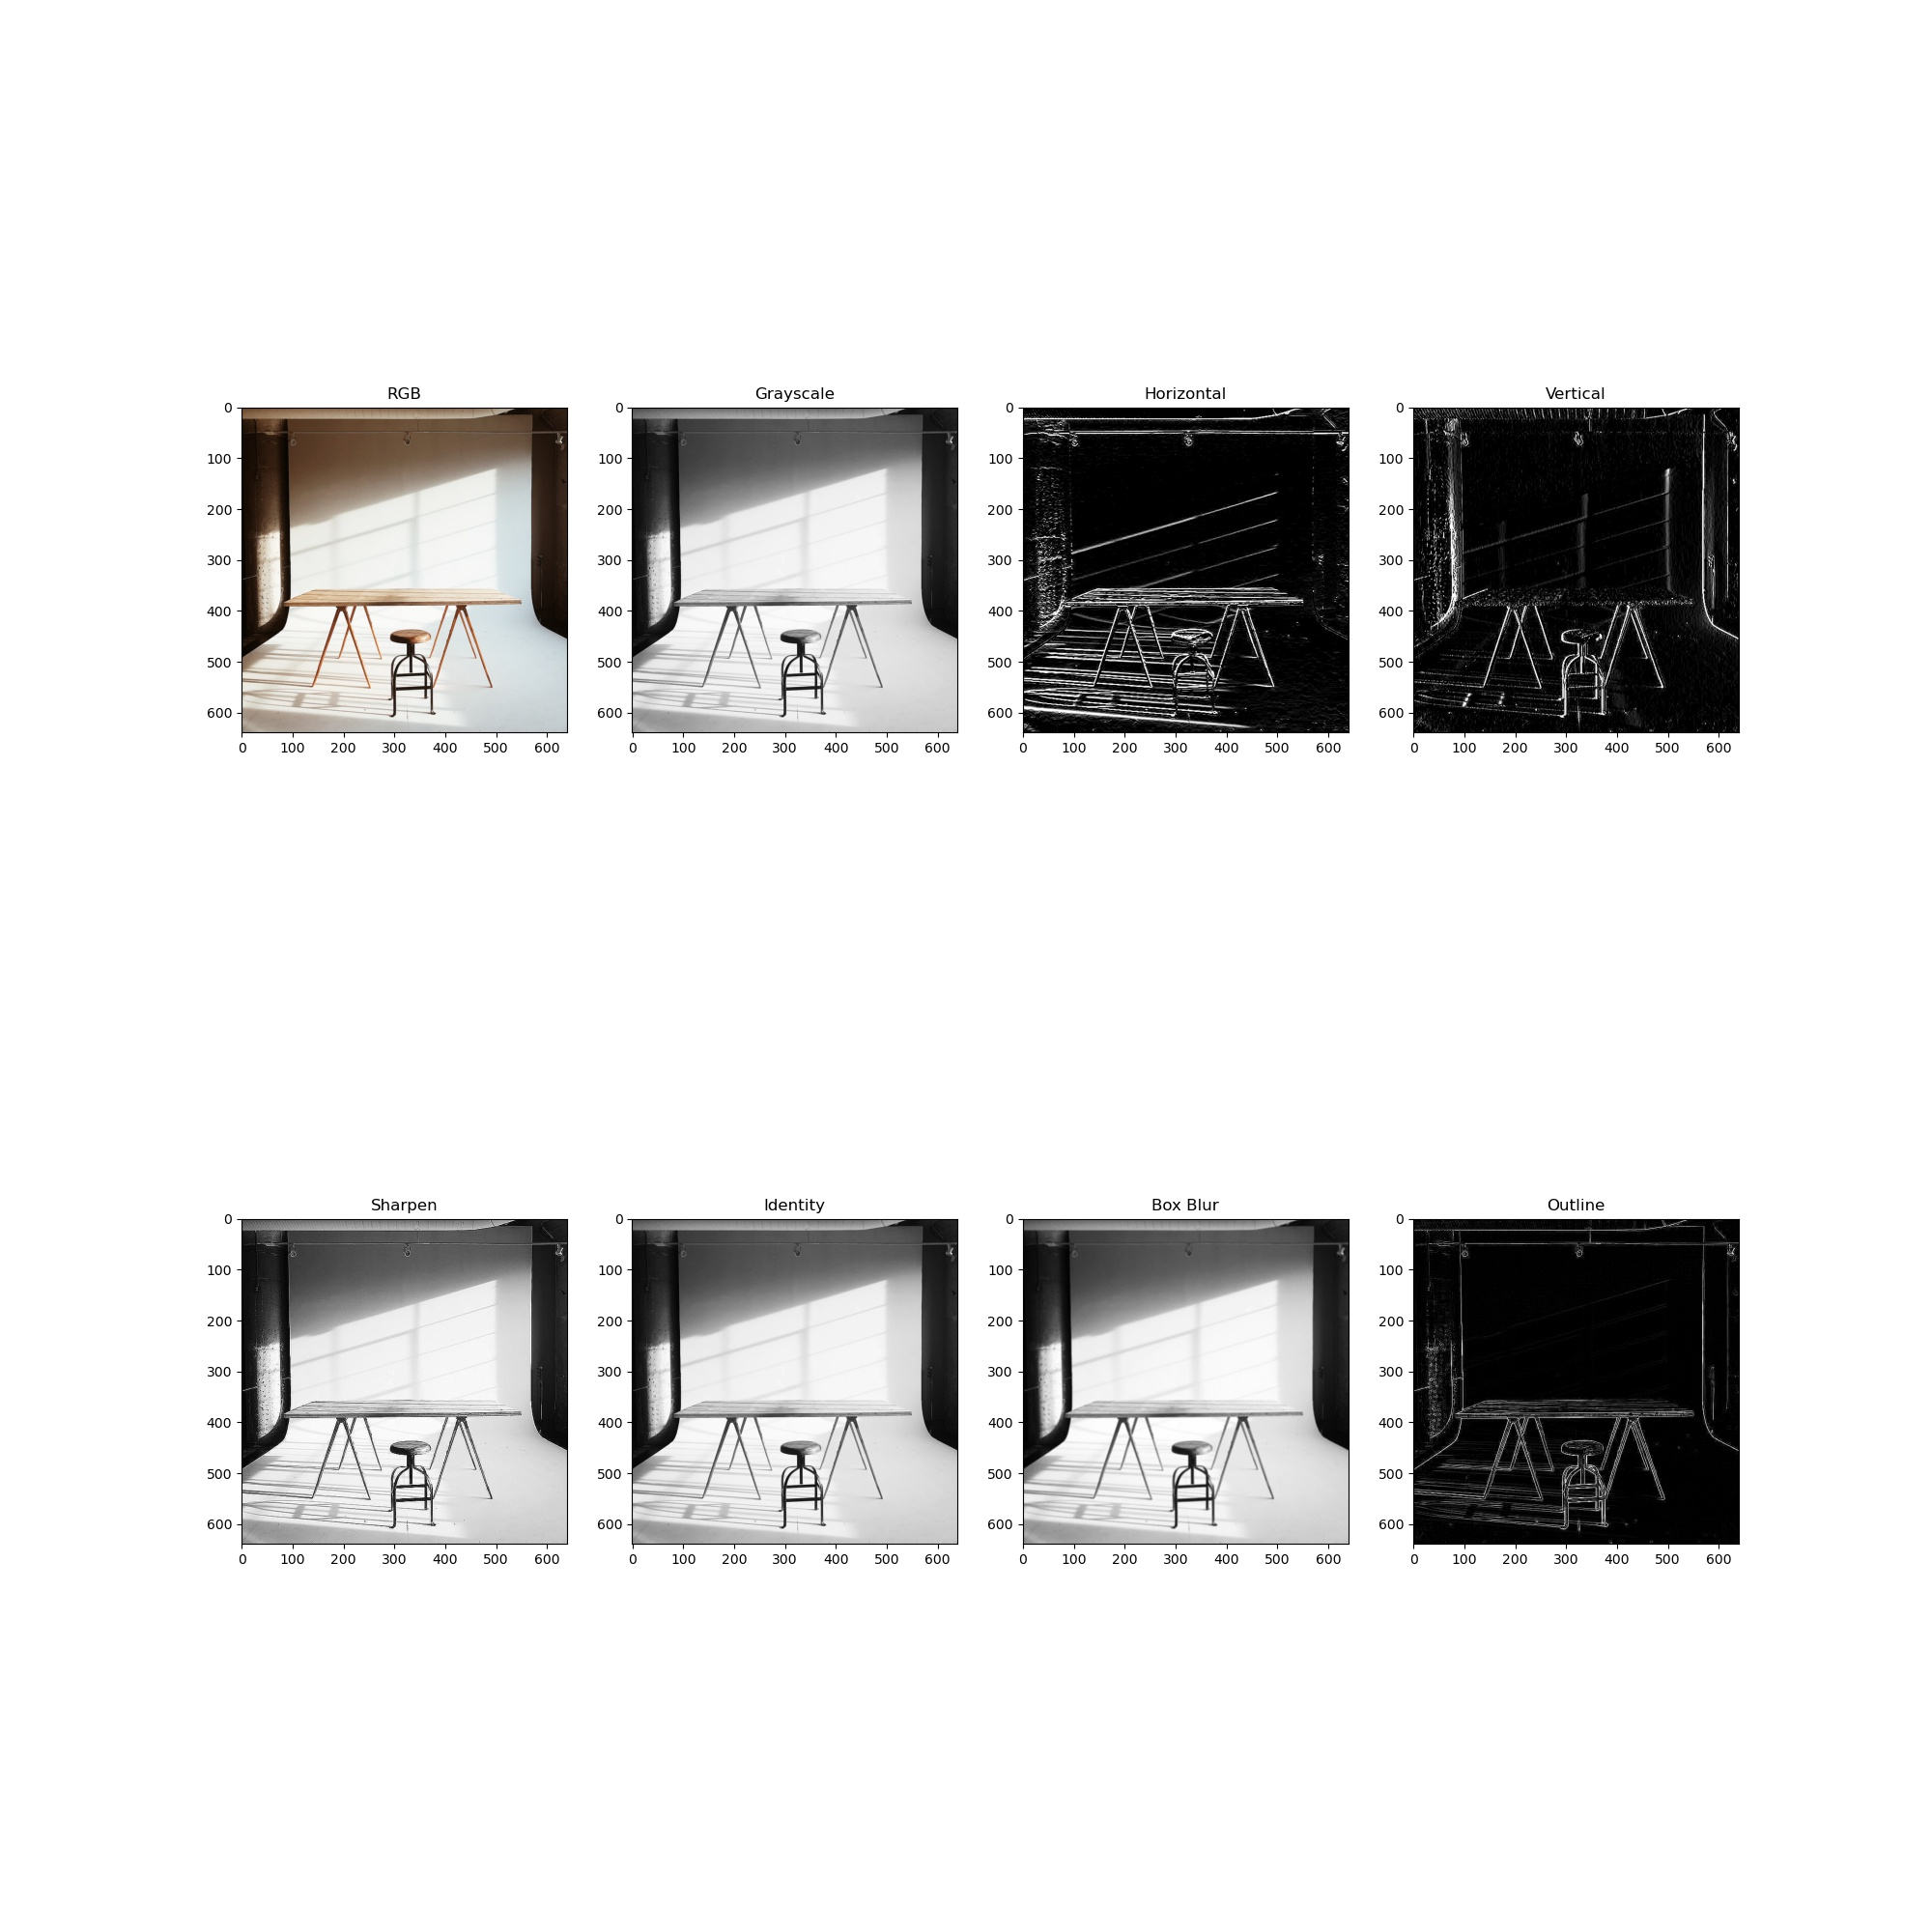
\includegraphics[width=0.5\textwidth]{Assignment-3/fig-1.jpg}
            \caption{Input image and output images of point processing}
        \end{figure}
    }
}
% \pagebreak
\clearpage

%-----------------------Assignment-4--------------------------%
{
    \section{Assignment-4}
    \subsection{Introduction}
    \textbf {Problem: }
    Perform the following task:\\
    1. Implement histogram and compare the result with built-in histogram function.\\
    2. Implement neighborhood processing and compare the result with built-in cv2.filter2D.\\
    \\
    \textbf{Solution: }
    Here, we have to do two task, at first, we have to implement the histogram function and then compare the histogram function with the built-in histogram function, performing operation on a same image. Secondly, on the same way, we have to implement the filtering function (neighbourhood processing) and then compare the filtering function with the built-in filtering function, performing operation on a same image. To do this, the following two program are used. Fist one for histogram and second one for filtering.
    \\
    
    \subsection{Required Software}
    For completing this task, we have to install open-cv, matplotlib and numpy. In our programs, we have to import the open-cv(cv2), matplotlib.pyplot as plt and numpy as np. We can install this three libraries using pip3. For different operations open-cv(cv2), numpy and matplotlib will have to be used - specially matplotlib for plotting and saving image. 
    \\
    
    \subsection{Procedure}
    \textbf{For implementing filtering function}\\
    \textbf{Step-1:}
    Install matplotlib, open-cv, numpy libraries.\\
    \textbf{Step-2:}
    Import them in our program. (matplotlib.pyplot as plt, cv2 as cv, numpy as np)\\
    \textbf{Step-3:}
    Read the RGB image and convert it to grayscale using cv.cvtColor() function.\\
    \textbf{Step-4:}
    Implement the filtering function using neighbourhood processing where the parameters are given grayscale image and kernel. Based on a center point, the convolution of image and kernel/filter is performed.\\
    \textbf{Step-5:}
    Perform the filtering operation on a same image using the built-in function and implemented function. Save the output.\\
    \textbf{Step-6:}
    Plot all the required images and save them as required in the question.\\
    
    \textbf{For implementing histogram function}\\
    \textbf{Step-1:}
    Install matplotlib, open-cv, numpy libraries.\\
    \textbf{Step-2:}
    Import them in our program. (matplotlib.pyplot as plt, cv2 as cv, numpy as np)\\
    \textbf{Step-3:}
    Read the RGB image and separate the image into three different channels - red, green, blue.\\
    \textbf{Step-4:}
    Implement the histogram function using frequency count of an image where the only parameter is the given grayscale image. Based this, the calculation is performed.\\
    \textbf{Step-5:}
    Perform the histogram operation on a same image using the built-in function and implemented function. Save the output.\\
    \textbf{Step-6:}
    Plot all the required images and save them as required in the question.\\
    
    \subsection{Code}
    \lstset{style=mystyle}
    \begin{lstlisting}[language=Python, caption=Code for implementing filtering function and compare it with built-in function]
    import matplotlib.pyplot as plt
    import cv2 as cv
    import numpy as np
    
    def main():
        img_path = './table.jpg'
        print(img_path)
        rgb = plt.imread(img_path)
        print(rgb.shape)
    
        grayscale = cv.cvtColor(rgb, cv.COLOR_RGB2GRAY)
    
        kernel1 = np.ones((3, 3), dtype = np.uint8)
        kernel2 = np.array([[3, 10, 3],[0, 0, 0], [-3, -10, -3]])
    
        processed_img11 = cv.filter2D(grayscale, -1, kernel1)
        processed_img12 = convolution(grayscale, kernel1)
    
        processed_img21 = cv.filter2D(grayscale, -1, kernel2)
        processed_img22 = convolution(grayscale, kernel2)
    
        img_set = [processed_img11, processed_img21, processed_img12, processed_img22]
        img_title = ['Blur1', 'Horizontal1', 'Blur2', 'Horizontal2']
    
        plt.figure(figsize = (20, 20))
        for i in range(len(img_set)):
            plt.subplot(2, 2, i+1)
            plt.title(img_title[i])
            plt.imshow(img_set[i], cmap = 'gray')
    
        plt.savefig('filter.jpg')
        plt.show()
    
    def convolution(img, kernel):
        processed_img = np.zeros((img.shape[0]-2, img.shape[1]-2))
        for i in range(img.shape[0]-2):
            for j in range(img.shape[1]-2):
                temp = np.sum(img[i:3+i, j:3+j] * kernel)
                if (temp > 255):
                    processed_img[i][j] = 255
                elif (temp < 0):
                    processed_img[i][j] = 0
                else: 
                    processed_img[i][j] = temp
        
        return processed_img
    
    if __name__ == '__main__':
        main()

    \end{lstlisting}
    \\
    \lstset{style=mystyle}
    \begin{lstlisting}[language=Python, caption=Code for implementing histogram function and compare it with built-in function]
    import matplotlib.pyplot as plt
    import cv2 as cv
    import numpy as np
            
    def main():
        img_path = './table.jpg'
        print(img_path)
        rgb = plt.imread(img_path)
        print(rgb.shape)
    
        red = rgb[:, :, 0]
        green = rgb[:, :, 1]
        blue = rgb[:, :, 2]
    
        histRed = cv.calcHist([rgb], [0], None, [256], [0, 256])
        histGreen = cv.calcHist([rgb], [1], None, [256], [0, 256])
        histBlue = cv.calcHist([rgb], [2], None, [256], [0, 256])
    
        histRed2 = histogram(red)
        histGreen2 = histogram(green)
        histBlue2 = histogram(blue)
    
        set_histogram = [histRed, histGreen, histBlue, [], histRed2, histGreen2, histBlue2, []]
        set_title = ['Red', 'Green', 'Blue', 'RGB', 'Red', 'Green', 'Blue', 'RGB']
        
        plt.figure(figsize = (20, 20))
        for i in range(len(set_histogram)):
            plt.subplot(2, 4, i+1)
            plt.title(set_title[i])
            if (i  == 3 or i == 7):
                plt.plot(set_histogram[i-3], 'r')
                plt.plot(set_histogram[i-2], 'g')
                plt.plot(set_histogram[i-1], 'b')
            else:
                plt.plot(set_histogram[i])
        plt.savefig('histogram.jpg')
        plt.show()
    
    def histogram(arr):
        frequencyCount = np.arange(0, 256)
        frequencyCount[:] = 0
        # print(frequencyCount)
        # print(arr) 
    
        for i in range(arr.shape[0]):
            for j in range(arr.shape[1]):
                if (arr[i][j] != 0):
                    frequencyCount[arr[i][j]] += 1
        
        return frequencyCount     
    
    if __name__ == '__main__':
        main()

    \end{lstlisting}
    \\
    
    \subsection{Result & Discussion}{
        Here, as at first, we read/load the RGB image, convert it to grayscale, or separate it into three channels of red, green, blue. For filtering operation both the output image of implemented function and built-in function is shown vertically for comparison. In the same way the output image for histogram is saved for comparison and plot them as follows. Now, if we look at the images, we can see that, the difference between the images is unnoticeable. So, the tasks are completed and our implementations work accurately.
        
        \begin{figure}[htp]
            \centering
            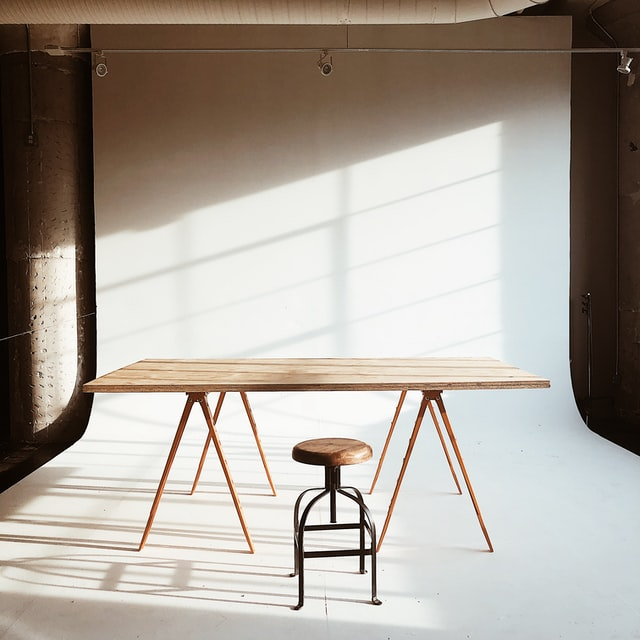
\includegraphics[width=0.6\textwidth]{Assignment-4/table.jpg}
            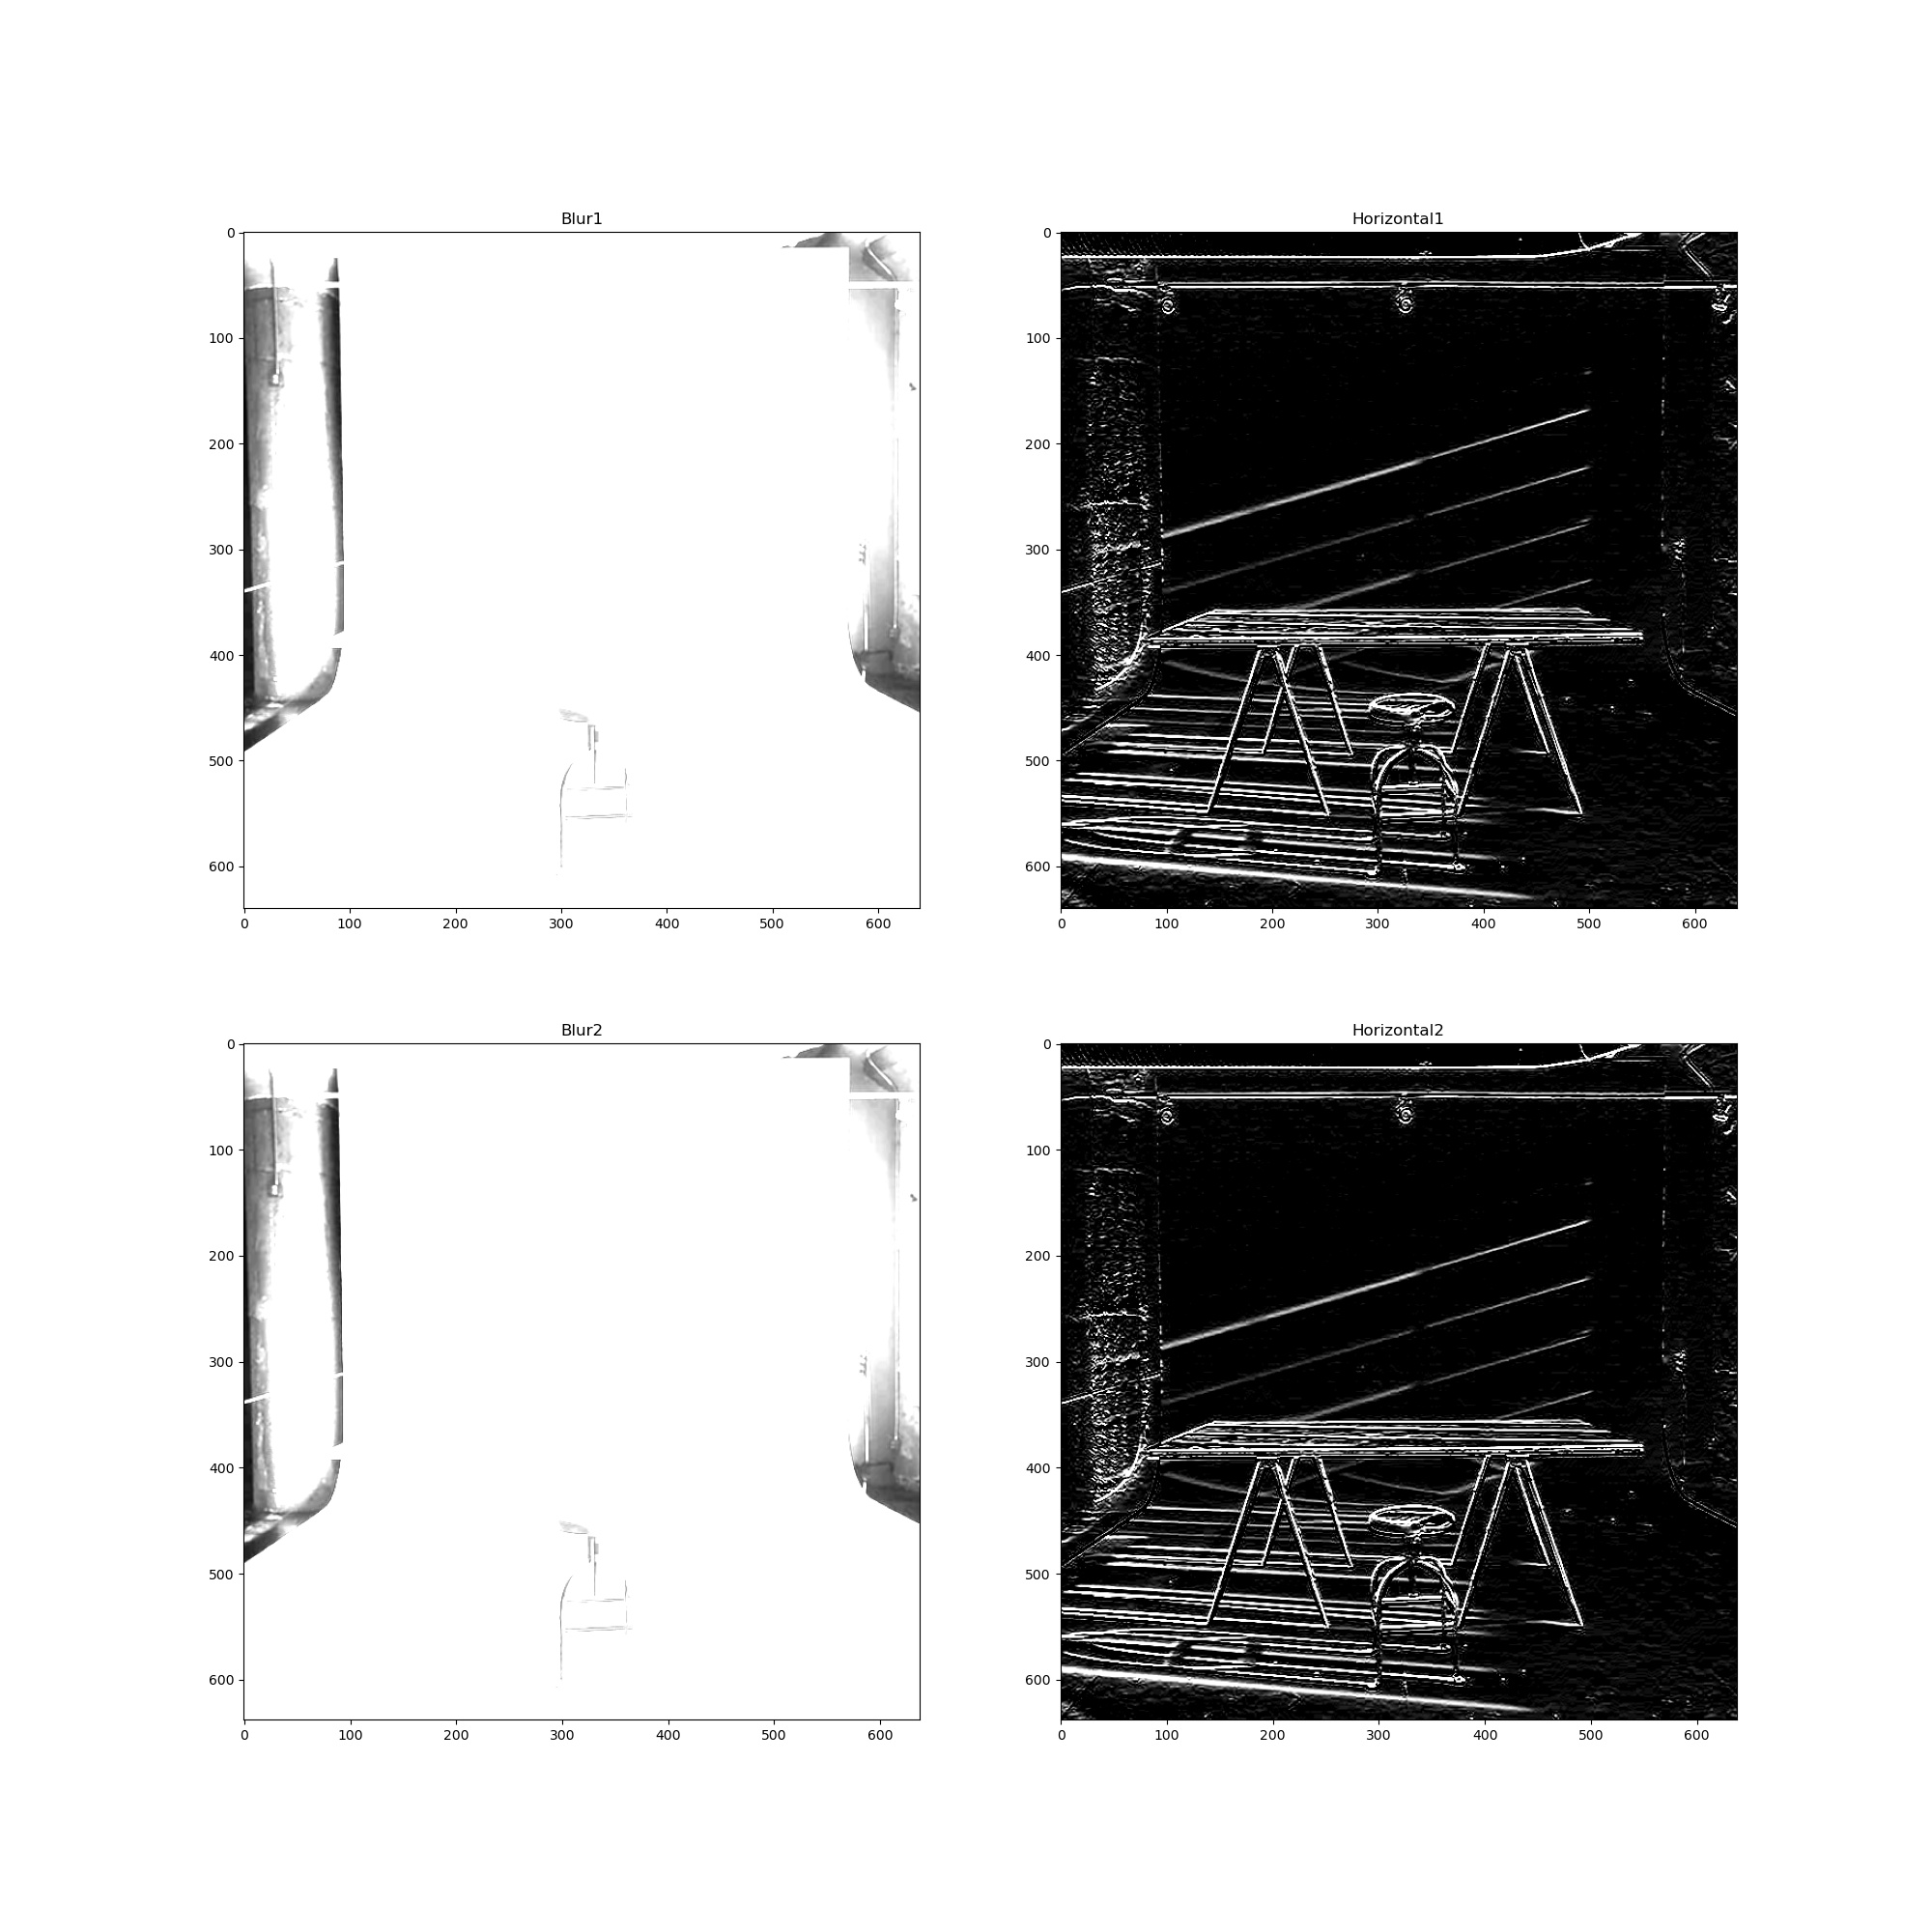
\includegraphics[width=0.49\textwidth]{Assignment-4/filter.jpg}
            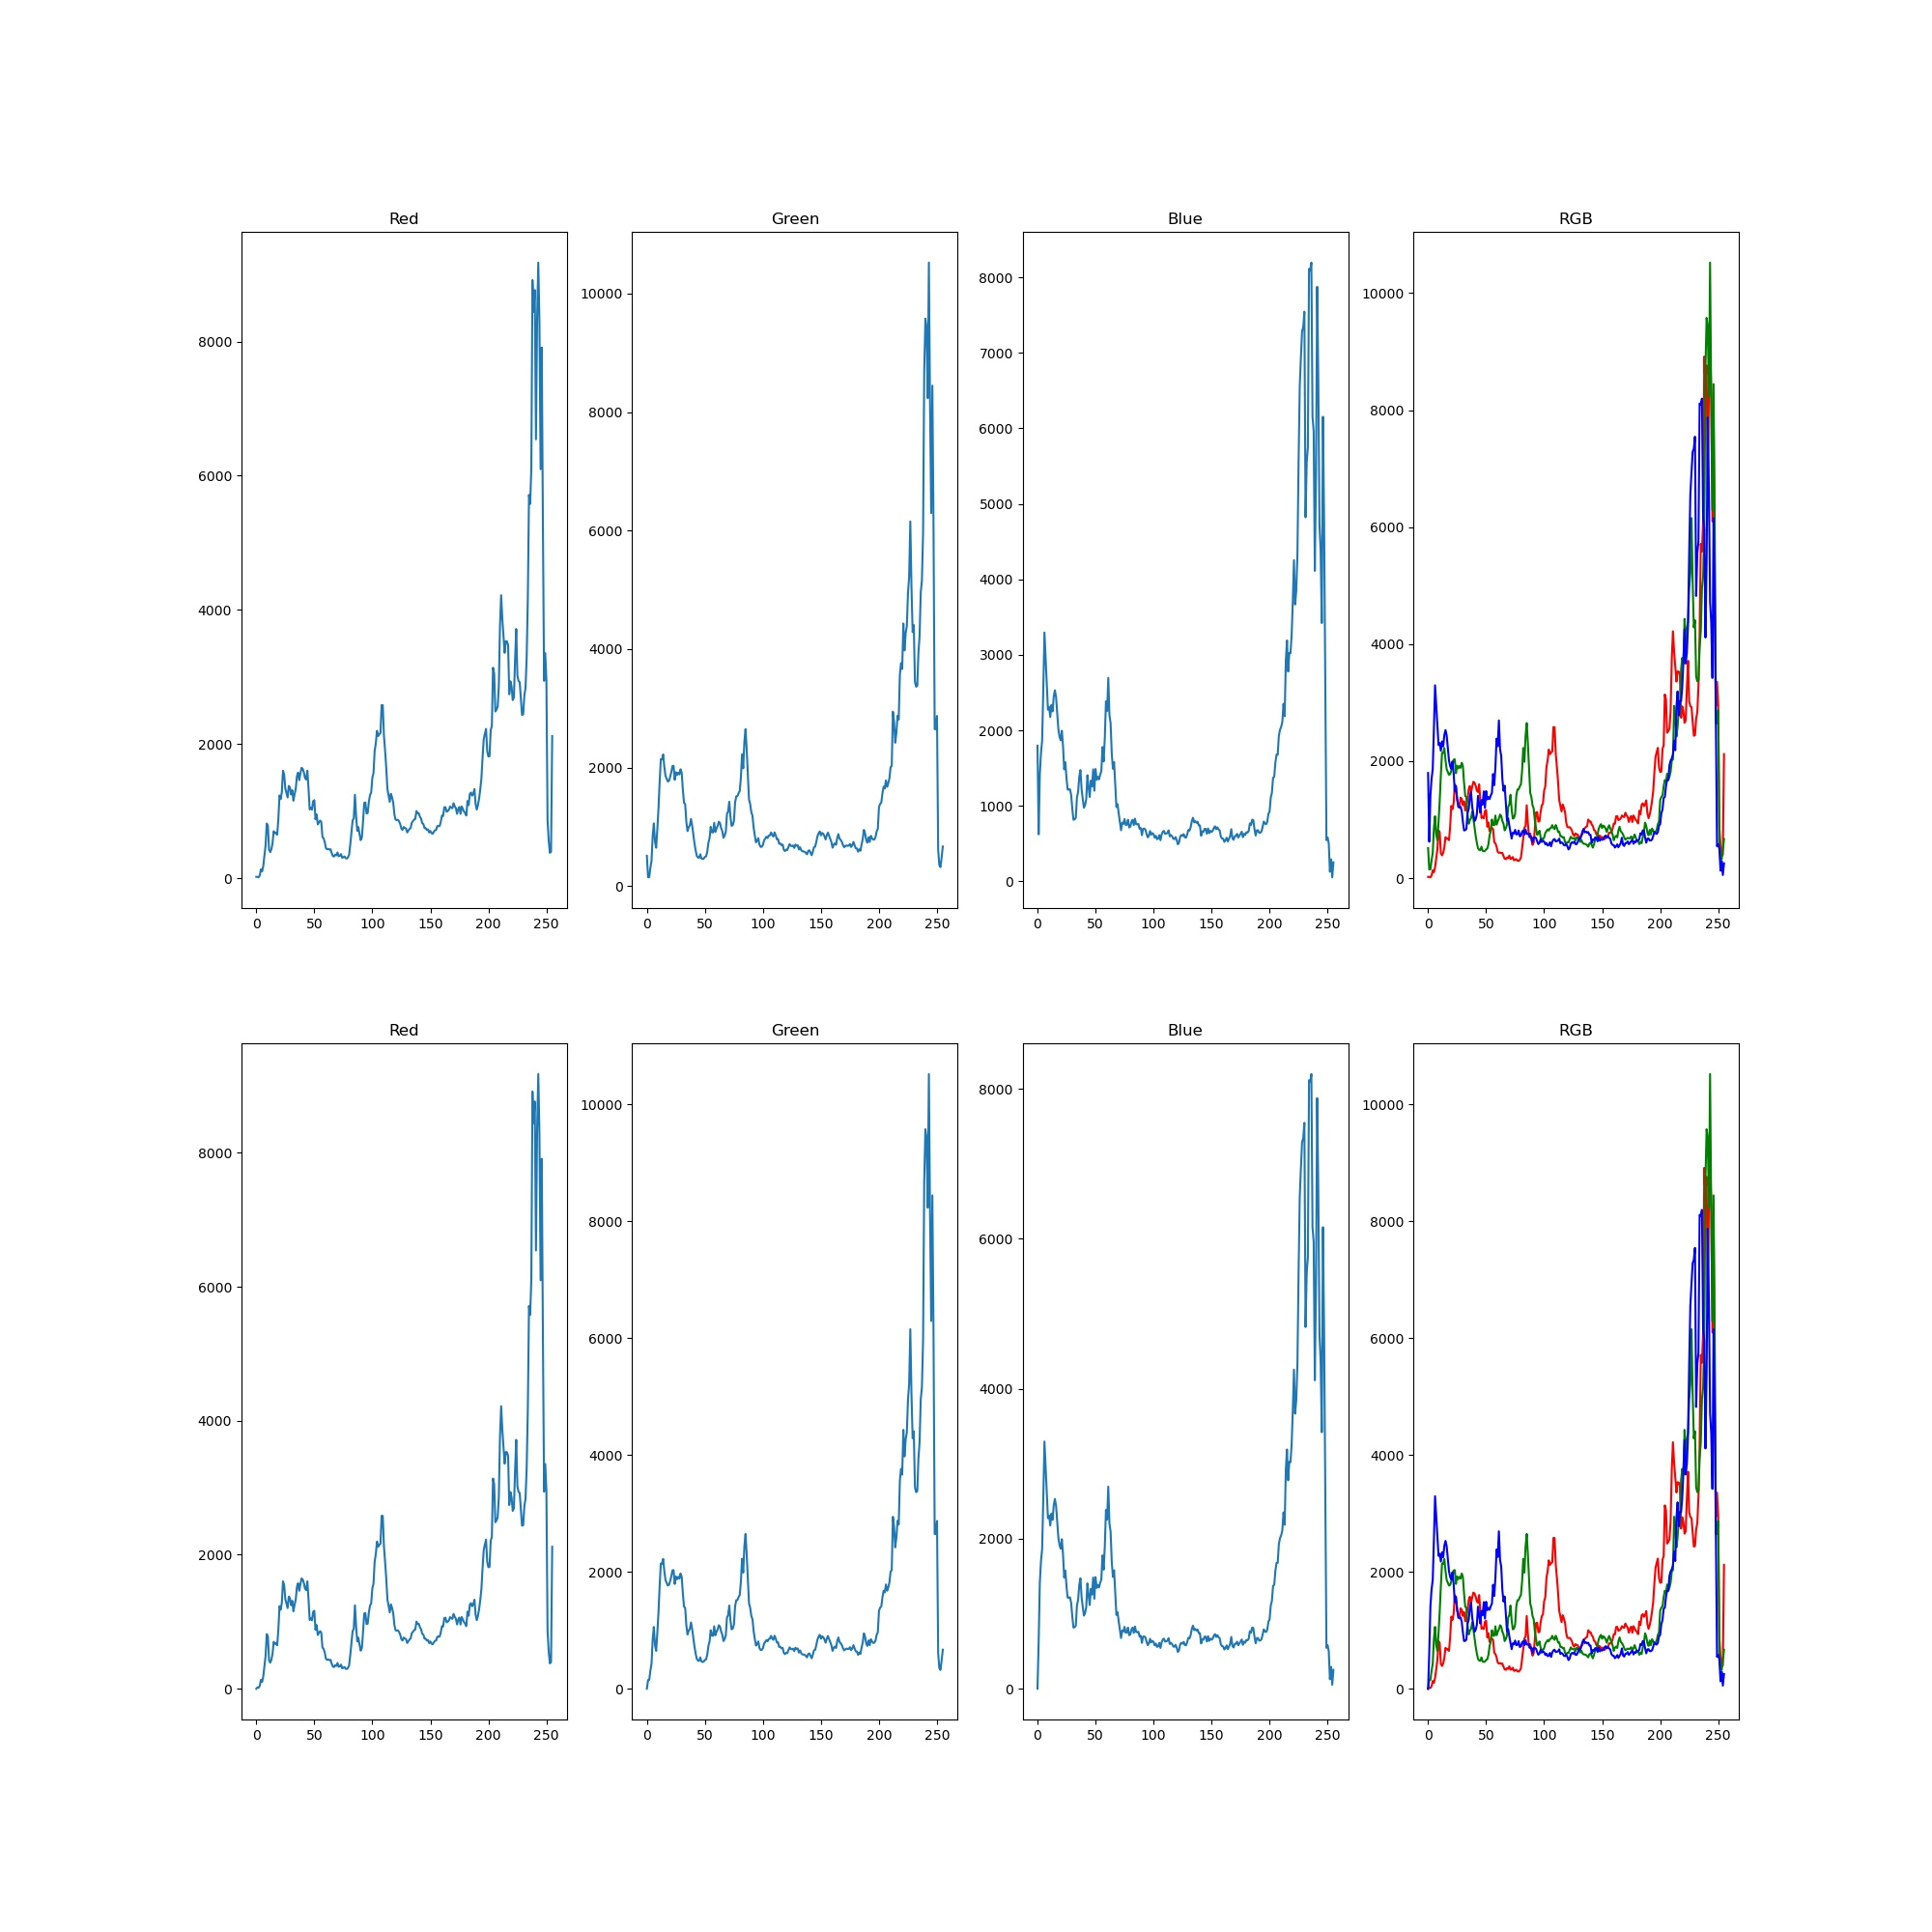
\includegraphics[width=0.49\textwidth]{Assignment-4/histogram.jpg}
            \caption{Input image, output images of filtering function, output image of histogram function}
        \end{figure}
    }
}
% \pagebreak
\clearpage

%-----------------------Assignment-5--------------------------%
{
    \section{Assignment-5}
    \subsection{Introduction}
    \textbf {Problem: }
    Perform the following task:\\
    1. Show what happens when we apply a binary mask on a grayscale image.\\
    2. Slice an 8-bit grayscale image into 8 planes.\\
    3. Show the effect of convolution of a grayscale image with a Laplacian filters and sobel filters.\\
    \\
    \textbf{Solution: }
    Here, we have to perform three tasks, at first, we have to check the output of applyng a binary mask on a grayscale image. Secondly, we have to slice a 8-bit grayscale image into 8 different planes. Thirdly, show the effect of convolution performing on a grayscale image with Laplacian filters and sobel filters. To do this, the following three program are used. First one for binary masking, second one for bit plane slicing and third one for performing convolution on a grayscale image using Laplacian and sobel filters.
    \\
    
    \subsection{Required Software}
    For completing this task, we have to install open-cv, matplotlib and numpy. In our programs, we have to import the open-cv(cv2), matplotlib.pyplot as plt and numpy as np. We can install this three libraries using pip3. For different operations open-cv(cv2), numpy and matplotlib will have to be used - specially matplotlib for plotting and saving image. 
    \\
    
    \subsection{Procedure}
    \textbf{For binary masking}\\
    \textbf{Step-1:}
    Install matplotlib, open-cv, numpy libraries.\\
    \textbf{Step-2:}
    Import them in our program. (matplotlib.pyplot as plt, cv2 as cv, numpy as np)\\
    \textbf{Step-3:}
    Read the RGB image and convert it to grayscale using cv.cvtColor() function.\\
    \textbf{Step-4:}
    Create two binary mask - one containing the value of 1 and other containing the value of 0.\\
    \textbf{Step-5:}
    Perform the AND operation on the image using the binary mask. Save the output.\\
    \textbf{Step-6:}
    Plot all the required images and save them as required in the question.\\
    
    \textbf{For bit plane slicing}\\
    \textbf{Step-1:}
    Install matplotlib, open-cv, numpy libraries.\\
    \textbf{Step-2:}
    Import them in our program. (matplotlib.pyplot as plt, cv2 as cv, numpy as np)\\
    \textbf{Step-3:}
    Read the RGB image and convert it to grayscale using cv.cvtColor() function.\\
    \textbf{Step-4:}
    Now for bit slicing, create 8 different variables containing the values of 1 to 128.\\
    \textbf{Step-5:}
    Perform the AND operation on the image with the 8 saved variables. Save the output.\\
    \textbf{Step-6:}
    Plot all the required images and save them as required in the question.\\
    
    \textbf{For laplace and sobel filtering}\\
    \textbf{Step-1:}
    Install matplotlib, open-cv, numpy libraries.\\
    \textbf{Step-2:}
    Import them in our program. (matplotlib.pyplot as plt, cv2 as cv, numpy as np)\\
    \textbf{Step-3:}
    Read the RGB image and convert it to grayscale using cv.cvtColor() function.\\
    \textbf{Step-4:}
    Create different laplace filters and sobel filters and save them.\\
    \textbf{Step-5:}
    Perform the filtering operation on the image with saved filter using cv.filter2D() function. Save the output.\\
    \textbf{Step-6:}
    Plot all the required images and save them as required in the question.\\
    
    \subsection{Code}
    \lstset{style=mystyle}
    \begin{lstlisting}[language=Python, caption=Code for binary masking a grayscale image]
    import matplotlib.pyplot as plt
    import numpy as np
    import cv2 as cv
    
    def main():
        img_path = './trees_in_water_3.jpg'
        print(img_path)
        rgb = plt.imread(img_path)
        print(rgb.shape)
    
        grayscale = cv.cvtColor(rgb, cv.COLOR_RGB2GRAY)
        print(grayscale.shape)
    
        mask = np.zeros((grayscale.shape[0], grayscale.shape[1]), dtype = np.uint8)
        mask[200:350, 50:300] = 255
    
        processed_img1 = np.zeros((grayscale.shape[0], grayscale.shape[1]), dtype = np.uint8)
        processed_img1 = grayscale & mask
        
        binaryMask = np.zeros((grayscale.shape[0], grayscale.shape[1]), dtype = np.uint8)
        binaryMask[200:350, 50:300] = 1
    
        processed_img2 = np.zeros((grayscale.shape[0], grayscale.shape[1]), dtype = np.uint8)
        processed_img2 = grayscale & binaryMask
    
        img_set = [rgb, grayscale, processed_img1, processed_img2]
        img_title = ['RGB', 'Gray', 'Masked Image', 'Binary Masked Image']
    
        plt.figure(figsize = (20, 20))
        for i in range(len(img_set)):
            plt.subplot(2, 2, i+1)
            plt.title(img_title[i])
            if (i == 0):
                plt.imshow(img_set[i])
            else:
                plt.imshow(img_set[i], cmap = 'gray')
    
        plt.savefig('mask-img.jpg')
        plt.show()
    
    if __name__ == "__main__":
        main()

    \end{lstlisting}
    \\
    \lstset{style=mystyle}
    \begin{lstlisting}[language=Python, caption=Code for bit slicing a grayscale image]
    import matplotlib.pyplot as plt
    import numpy as np
    import cv2 as cv
    
    def main():
        img_path = './trees_in_water_3.jpg'
        print(img_path)
        rgb = plt.imread(img_path)
        print(rgb.shape)
    
        grayscale = cv.cvtColor(rgb, cv.COLOR_RGB2GRAY)
        print(grayscale.shape)
    
        bit1_img = np.ones((grayscale.shape[0], grayscale.shape[1]), dtype = np.uint8)
        bit2_img = 2 * np.ones((grayscale.shape[0], grayscale.shape[1]), dtype = np.uint8)
        bit3_img = 4 * np.ones((grayscale.shape[0], grayscale.shape[1]), dtype = np.uint8)
        bit4_img = 8 *np.ones((grayscale.shape[0], grayscale.shape[1]), dtype = np.uint8)
        bit5_img = 16 * np.ones((grayscale.shape[0], grayscale.shape[1]), dtype = np.uint8)
        bit6_img = 32 * np.ones((grayscale.shape[0], grayscale.shape[1]), dtype = np.uint8)
        bit7_img = 64 * np.ones((grayscale.shape[0], grayscale.shape[1]), dtype = np.uint8)
        bit8_img = 128 * np.ones((grayscale.shape[0], grayscale.shape[1]), dtype = np.uint8)
            
        bit1_img = grayscale & bit1_img
        bit2_img = grayscale & bit2_img
        bit3_img = grayscale & bit3_img
        bit4_img = grayscale & bit4_img
        bit5_img = grayscale & bit5_img
        bit6_img = grayscale & bit6_img
        bit7_img = grayscale & bit7_img
        bit8_img = grayscale & bit8_img
        
        # bit2_img = np.zeros((grayscale.shape[0], grayscale.shape[1]), dtype = np.uint8)
        # for i in range(grayscale.shape[0]):
        #     for j in range(grayscale.shape[1]):
        #         bit2_img[i][j] = grayscale[i][j] & 1
        bit_img = [rgb, grayscale, bit1_img, bit2_img, bit3_img, bit4_img, bit5_img, bit6_img, bit7_img, bit8_img]
        bit_title = ['RGB', 'Gray','LSB', '2nd LSB', '3rd LSB', '4th LSB', '4th MSB', '3rd MSB', '2nd MSB', 'MSB'] 
        
        plt.figure(figsize = (20, 20))
        for i in range(len(bit_img)):
            plt.subplot(2, 5, i+1)
            plt.title(bit_title[i])
            if (i == 0):
                plt.imshow(bit_img[i])
            else :
                plt.imshow(bit_img[i], cmap = 'gray')
    
        plt.savefig('bit-wise-image.jpg')
        plt.show()
    
    
    if __name__ == "__main__":
        main()

    \end{lstlisting}
    \\
    \lstset{style=mystyle}
    \begin{lstlisting}[language=Python, caption=Code for laplacian filtering and sobel filtering on a grayscale image]
    import matplotlib.pyplot as plt
    import numpy as np
    import cv2 as cv
    
    def main():
        img_path = './trees_in_water_3.jpg'
        print(img_path)
        rgb = plt.imread(img_path)
        print(rgb.shape)
    
        grayscale = cv.cvtColor(rgb, cv.COLOR_RGB2GRAY)
        print(grayscale.shape)
    
        laplaceKernel1 = np.array([[0, 1, 0], [1, -4, 1], [0, 1, 0]])
        laplaceKernel2 = np.array([[0, -1, 0], [-1, 4, -1], [0, -1, 0]])
        laplaceKernel3 = np.array([[1, 1, 1], [1, -8, 1], [1, 1, 1]])
        laplaceKernel4 = np.array([[-1, -1, -1], [-1, 8, -1], [-1, -1, -1]])
    
        sobelKernel1 = np.array([[-1, -2, -1], [0, 0, 0], [1, 2, 1]])
        sobelKernel2 = np.array([[-1, 0, 1], [-2, 0, 2], [-1, 0, 1]])
    
        processed_img1 = cv.filter2D(grayscale, -1, laplaceKernel1)
        processed_img2 = cv.filter2D(grayscale, -1, laplaceKernel2)
        processed_img3 = cv.filter2D(grayscale, -1, laplaceKernel3)
        processed_img4 = cv.filter2D(grayscale, -1, laplaceKernel4)
    
        processed_img5 = cv.filter2D(grayscale, -1, sobelKernel1)
        processed_img6 = cv.filter2D(grayscale, -1, sobelKernel2)
    
        set_img = [rgb, grayscale, processed_img1, processed_img2, processed_img3, processed_img4, processed_img5, processed_img6]
        set_title = ['RGB', 'Gray', 'Laplace Kernel1', 'Laplace Kernel2', 'Laplace Kernel3', 'Laplace Kernel4', 'Sobel Kernel1', 'Sobel Kernel2']
    
        plt.figure(figsize = (20, 20))
        for i in range(len(set_img)):
            plt.subplot(2, 4, i+1)
            plt.title(set_title[i])
            if (i == 0):
                plt.imshow(set_img[i])
            else:
                plt.imshow(set_img[i], cmap = 'gray')
        plt.savefig('Laplace-&-Sobel-Filtering.jpg')
        plt.show()
    
    if __name__ == "__main__":
        main()

    \end{lstlisting}
    \\
    
    \subsection{Result & Discussion}{
        Here, as at first, we read/load the RGB image then convert it to grayscale. For binary masking, both the output of two differnt binary mask is saved in the first image as follows. For bit slicing, the output of 8 different images is saved in the second image as follows. In the same way, for laplacian filtering and sobel filtering, the outputs are shown in the third images as follows. Now, if we look at the images, we can see that, we get all the expected outputs for binary masking, bit plane slicing and laplace and sobel filtering. So, it can be said that the tasks are completed and our programs work accurately.
        
        \begin{figure}[htp]
            \centering
            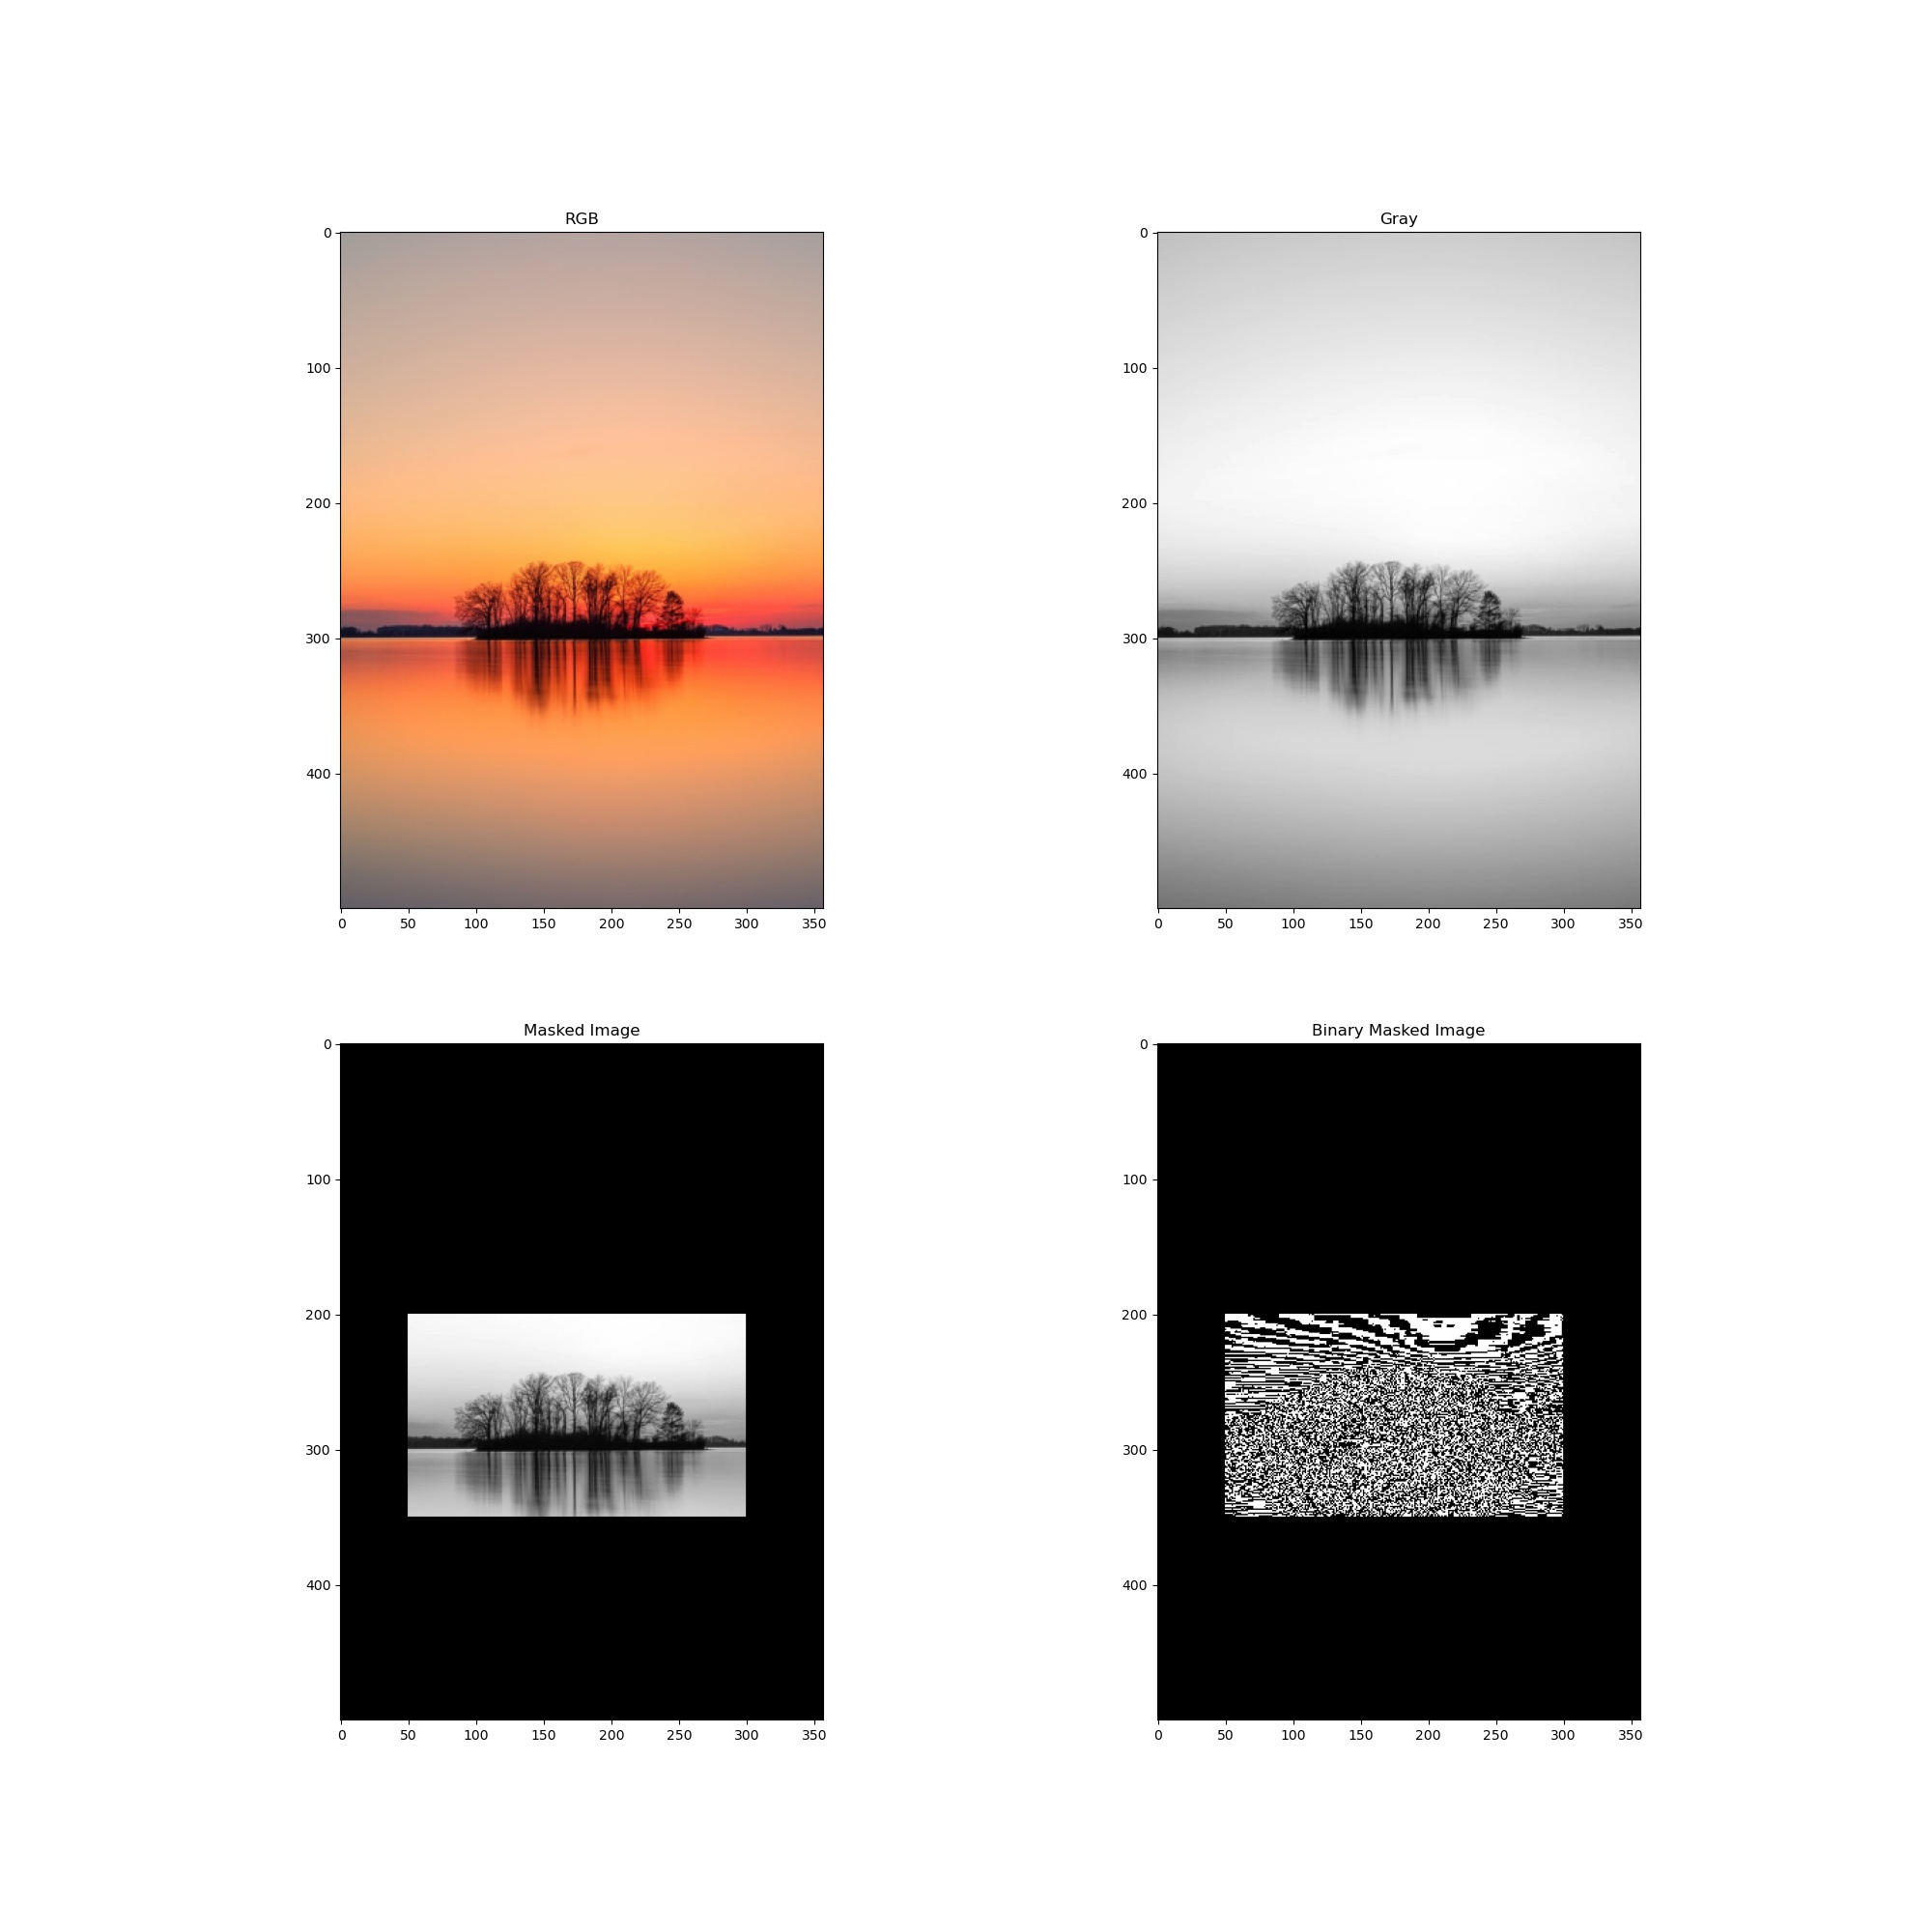
\includegraphics[width=0.49\textwidth]{Assignment-5/mask-img.jpg}
            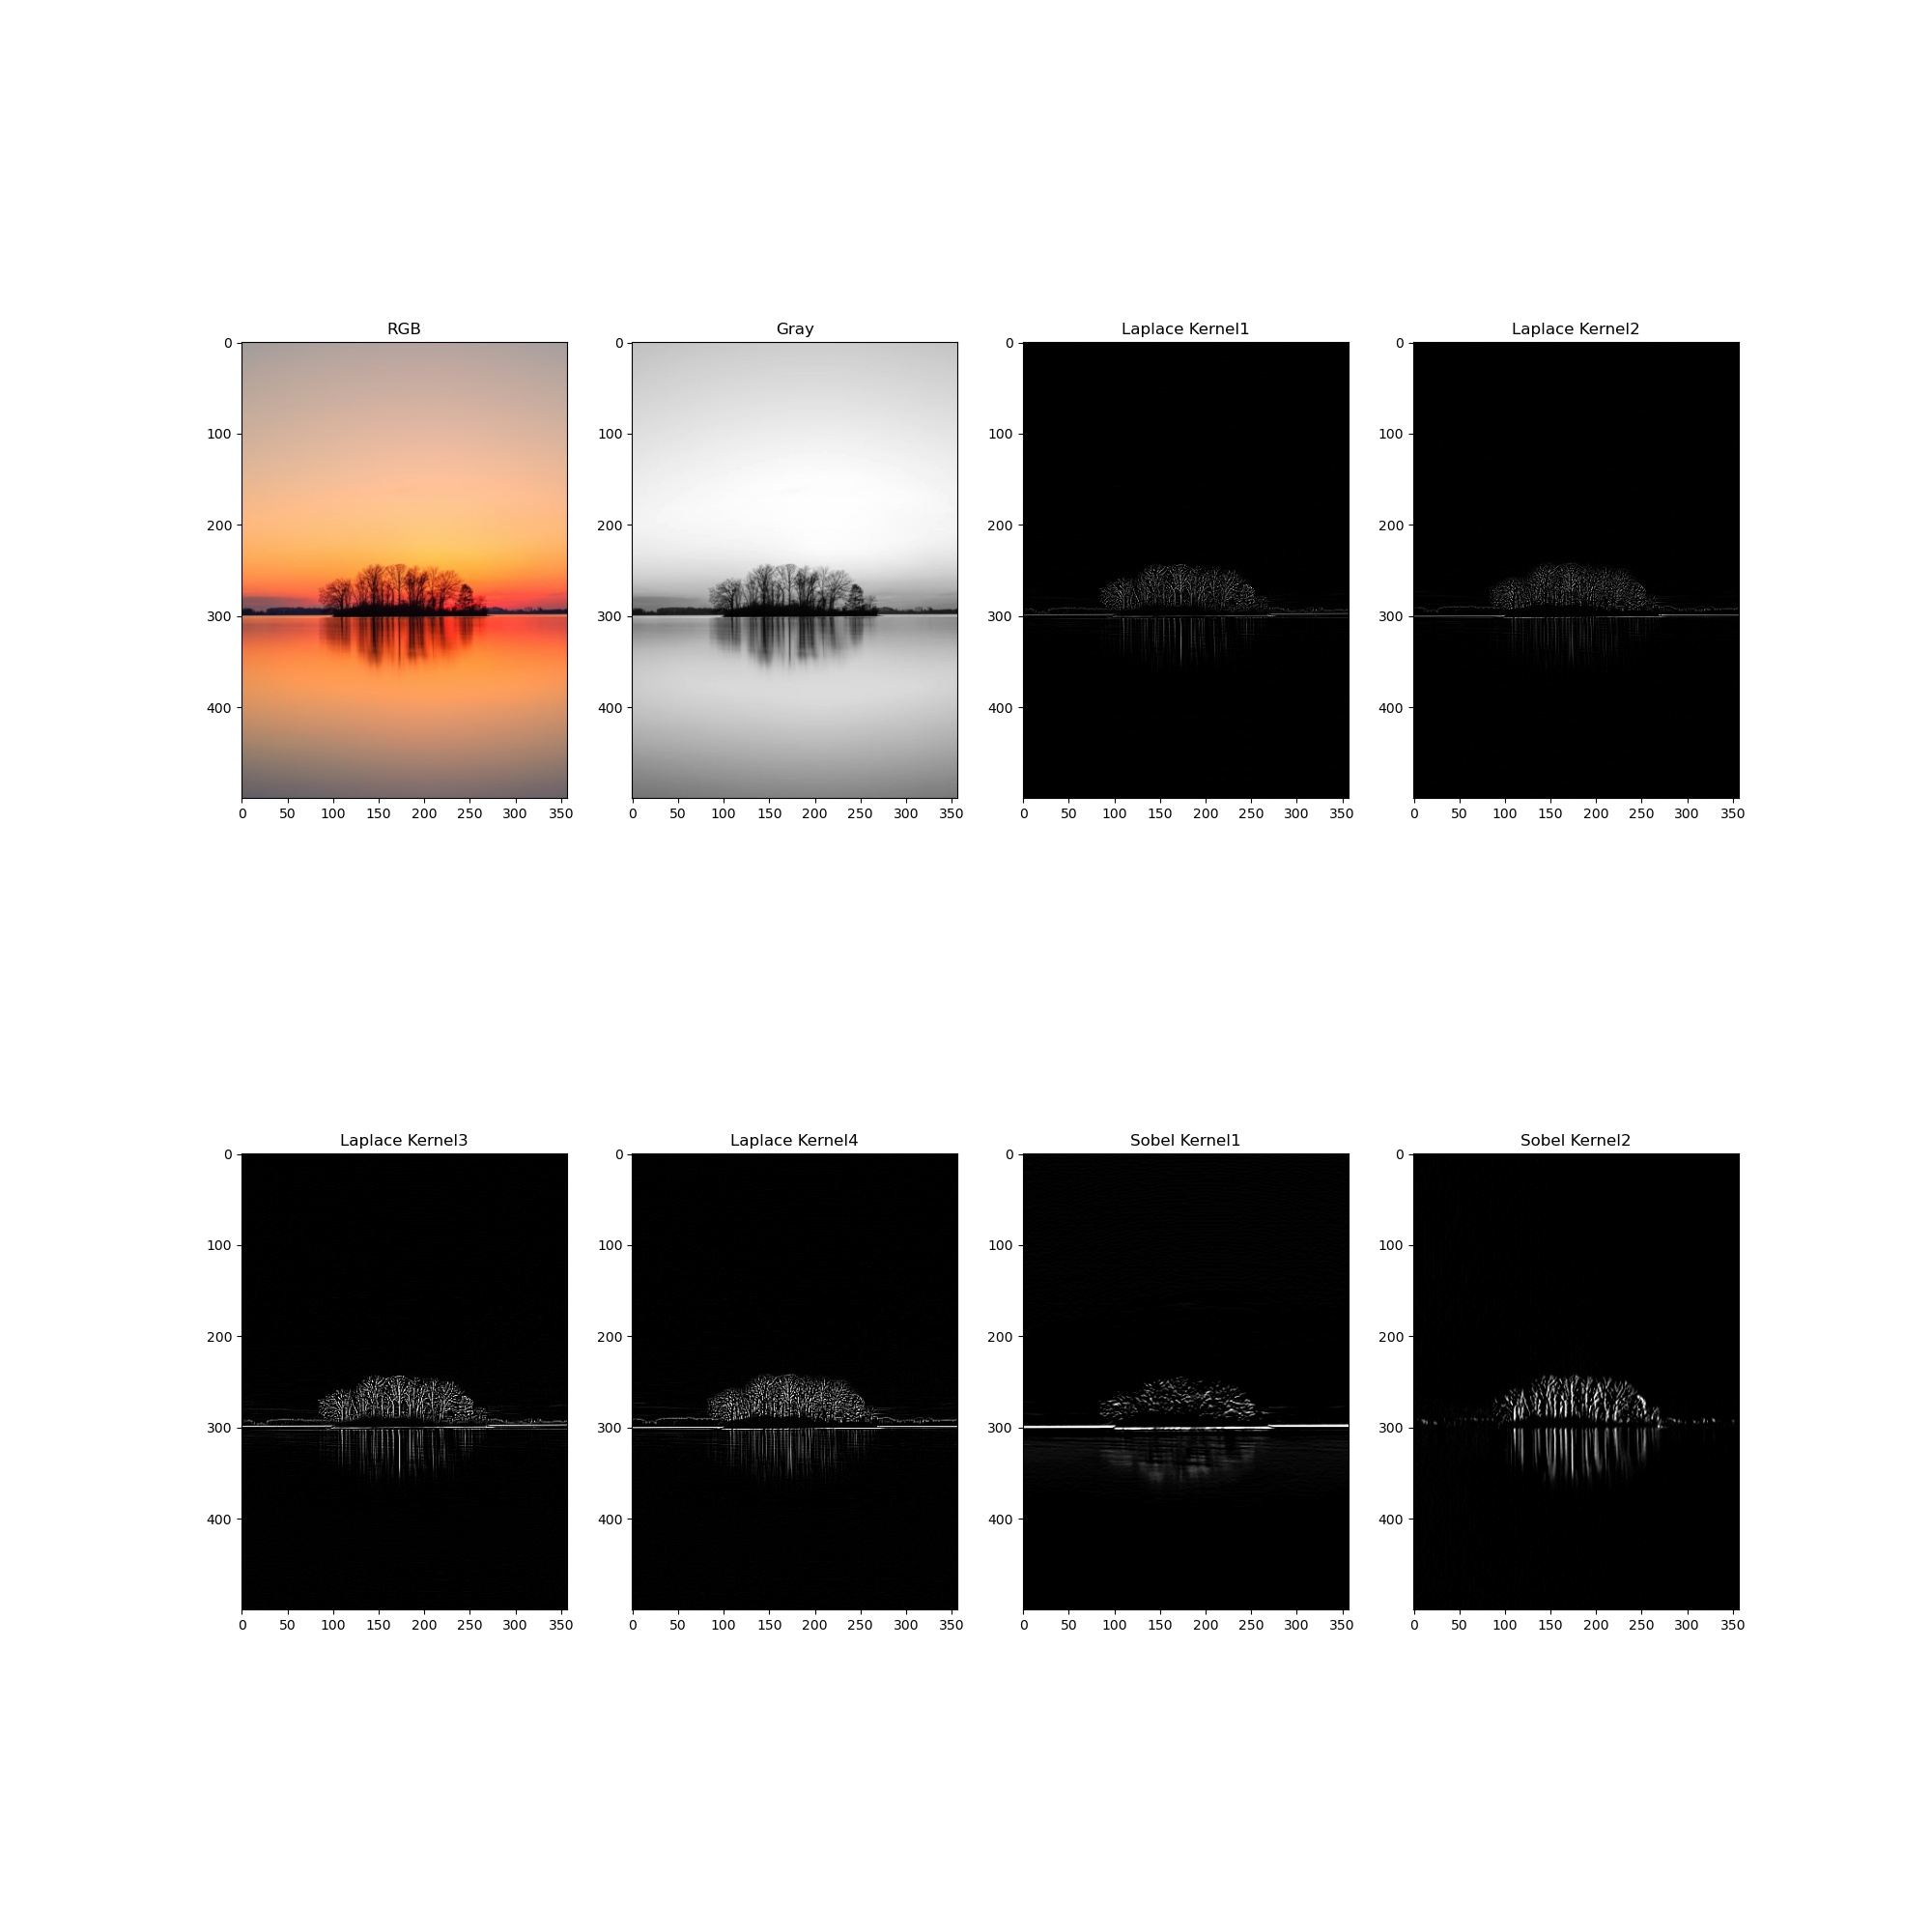
\includegraphics[width=0.49\textwidth]{Assignment-5/Laplace-&-Sobel-Filtering.jpg}
            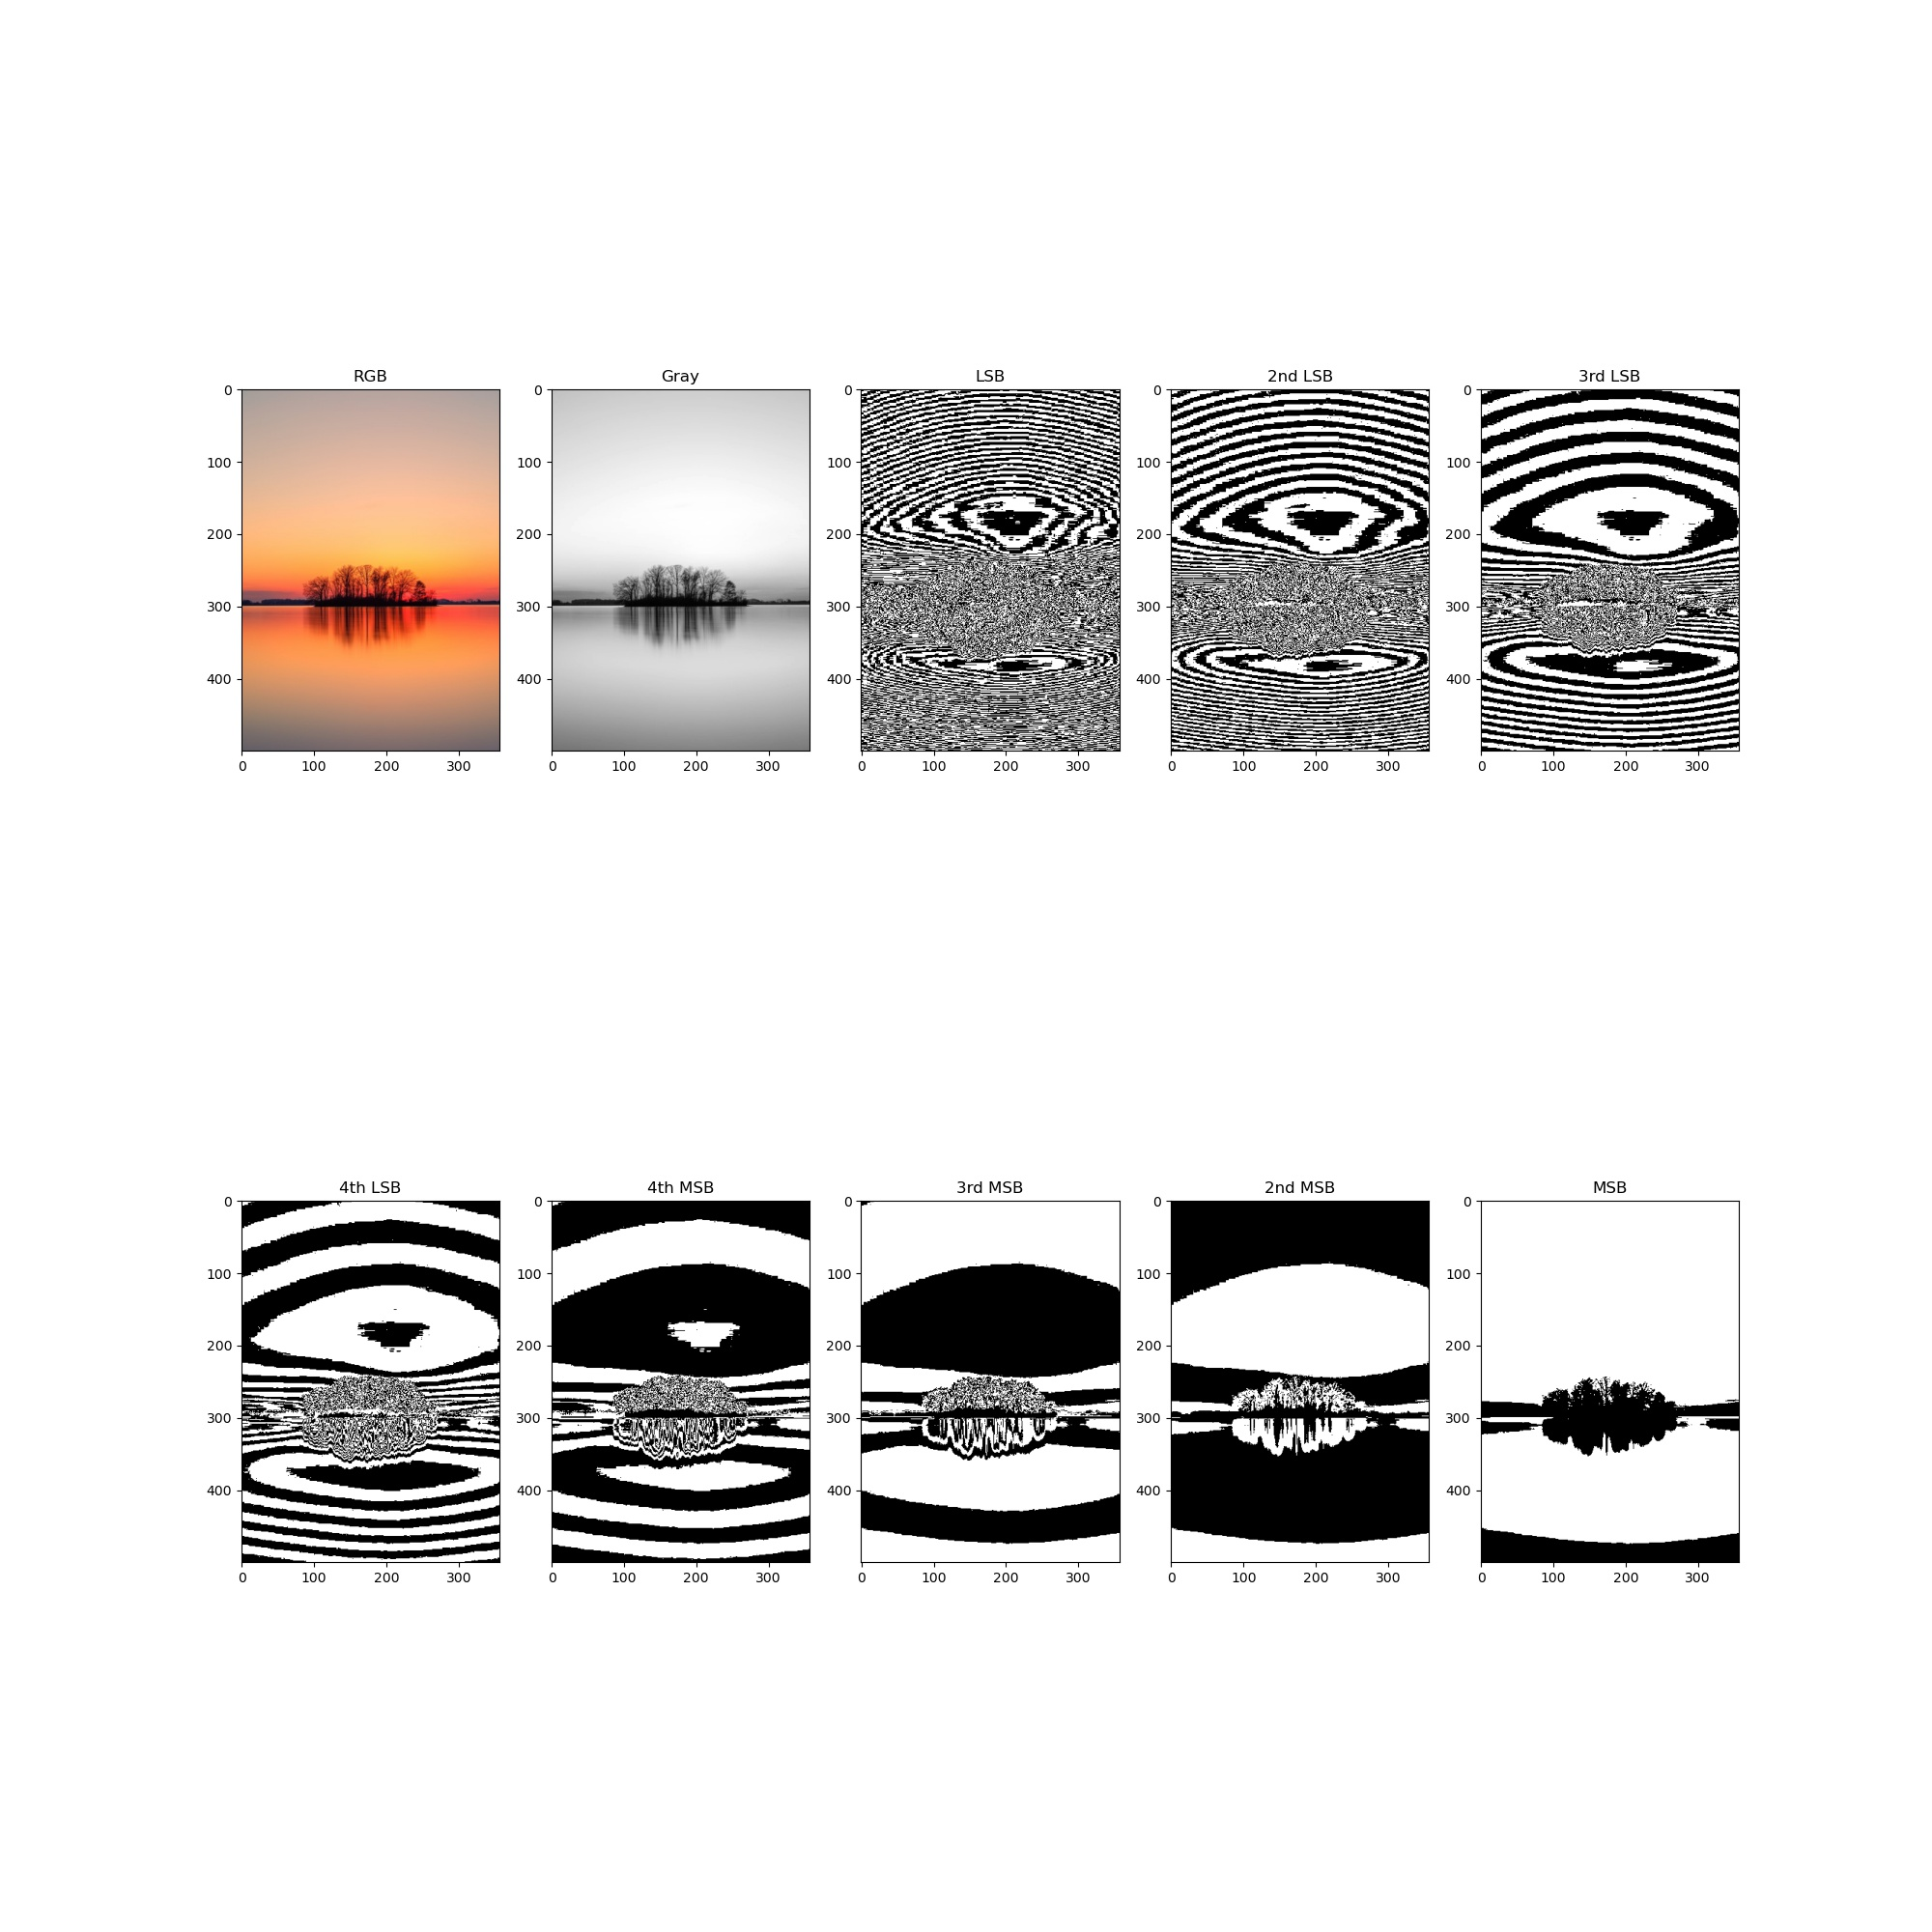
\includegraphics[width=0.8\textwidth]{Assignment-5/bit-wise-image.jpg}
            \caption{Input image and outputs of binary masking, Input image and outputs of laplace and sobel filtering, Input image and outputs of bit plane slicing}
        \end{figure}
    }
}
% \pagebreak
\clearpage

%-----------------------Assignment-6--------------------------%
{
    \section{Assignment-6}
    \subsection{Introduction}
    \textbf {Problem: }
    Add 'salt & pepper noise' with an image and see the effect of average kernel, Gaussian kernel and median filter on the noisy image. A sample output is attached.
    \begin{figure}[htp]
        \centering
        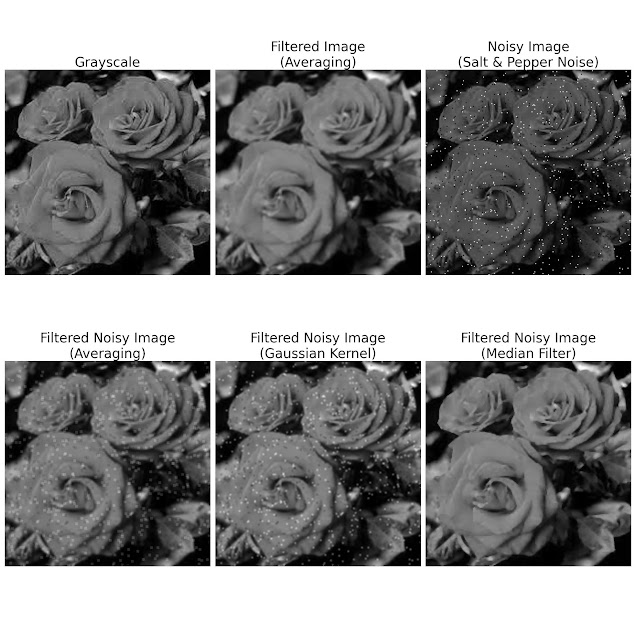
\includegraphics[width=0.5\textwidth]{Assignment-6/Salt_Pepper_Noisy_Rose.jpeg}
        \caption{salt and pepper noise sample}
    \end{figure}
    \\
    \\
    \textbf{Solution: }
    Here at first, we have to add salt and pepper noise to an image. Then we have to perform the filtering operation of average filter, Gaussian filter, median filter. We also have to discuss the output of the filtering effect of the noisy image. To perform the given task, the following program is used.
    \\
    
    \subsection{Required Software}
    For completing this task, we have to install open-cv, matplotlib and numpy. In our programs, we have to import the open-cv(cv2), matplotlib.pyplot as plt and numpy as np. We can install this three libraries using pip3. For different operations open-cv(cv2), numpy and matplotlib will have to be used - specially matplotlib for plotting and saving image. 
    \\
    
    \subsection{Procedure}
    \textbf{Step-1:}
    Install matplotlib, open-cv, numpy libraries.\\
    \textbf{Step-2:}
    Import them in our program. (matplotlib.pyplot as plt, cv2 as cv, numpy as np)\\
    \textbf{Step-3:}
    Read the RGB image and convert it to grayscale using cv.cvtColor() function.\\
    \textbf{Step-4:}
    Add salt and pepper noise randomly in the image.\\
    \textbf{Step-5:}
    Create the average filter, Gaussian filter and median filter with the help of numpy.\\
    \textbf{Step-6:}
    Perform the filtering operations on the image using the cv.filter2D() function. Save the outputs.\\
    \textbf{Step-7:}
    Plot all the required images and save them as required in the question.\\
    
    \subsection{Code}
    \lstset{style=mystyle}
    \begin{lstlisting}[language=Python, caption=Code for performing average filtering, Gaussian filtering and median filtering in a salt and pepper noisy image]
    import matplotlib.pyplot as plt
    import numpy as np
    import cv2 as cv
    
    def main():
        img_path = 'rose_2.jpg'
        print(img_path)
        rgb = plt.imread(img_path)
        print(rgb.shape)
    
        grayscale = cv.cvtColor(rgb, cv.COLOR_RGB2GRAY)
        print(grayscale.shape)
        
        avg_kernel = 1/9 * np.ones((3, 3))
        gaussian_kernel = 1/16 * np.array([[1, 2, 1], [2, 4, 2], [1, 2, 1]])
    
        processed_img = cv.filter2D(grayscale, -1, avg_kernel)
    
        noisy_img = np.copy(grayscale)
        for i in range(2000):
            x = np.random.randint(0, noisy_img.shape[0])
            y = np.random.randint(0, noisy_img.shape[1])
            noisy_img[x][y] = np.random.randint(0, 2) * 255
        
        processed_noisy_img1 = cv.filter2D(noisy_img, -1, avg_kernel)
        processed_noisy_img2 = cv.filter2D(noisy_img, -1, gaussian_kernel)
    
        # processed_noisy_img3 = np.zeros((noisy_img.shape[0], noisy_img.shape[1]))
        # for i in range(processed_noisy_img3.shape[0]-2):
        #     for j in range(processed_noisy_img3.shape[1]-2):
        #         processed_noisy_img3[i][j] = np.median(noisy_img[i:3+i, j:3+j])
    
        processed_noisy_img3 = cv.medianBlur(noisy_img, 3)
    
        img_set = [grayscale, processed_img, noisy_img, processed_noisy_img1, processed_noisy_img2, processed_noisy_img3]
        title_set = ['Gray', 'Filtered Image\n(Averaging)', 'Noisy Image\n(Salt & Pepper)', 'Filtered Noisy Image\n(Average Filter)', 'Filtered Noisy Image\n(Gaussian Filter)', 'Filtered Noisy Image\n(Median Filter)']
        
        plt.figure(figsize = (20, 20))
        for i in range(len(img_set)):
            plt.subplot(2, 3, i+1)
            plt.title(title_set[i])
            plt.imshow(img_set[i], cmap = 'gray')
    
        plt.savefig('noise.jpg')
        plt.show()
    
    if __name__ == "__main__":
        main()

    \end{lstlisting}
    \\
    
    \subsection{Result & Discussion}{
        Here, as at first, we read/load the RGB image then convert it to grayscale. Then we add salt and pepper noise in the image. After that we apply averaging filtering, Gaussian filtering and median filtering on that image. The outputs of these operations are given as follows. From the outputs, we can see that, for average filtering, the noise is somewhat removed but not totally removed. Again for Gaussian filtering, we get a slightly better result but not all noise is removed. After that, when we apply median filtering, we get to see that the noise is removed and the image becomes smooth. As we get the expected output, so it can be said that the task is completed and our program works accurately.
        
        \begin{figure}[htp]
            \centering
            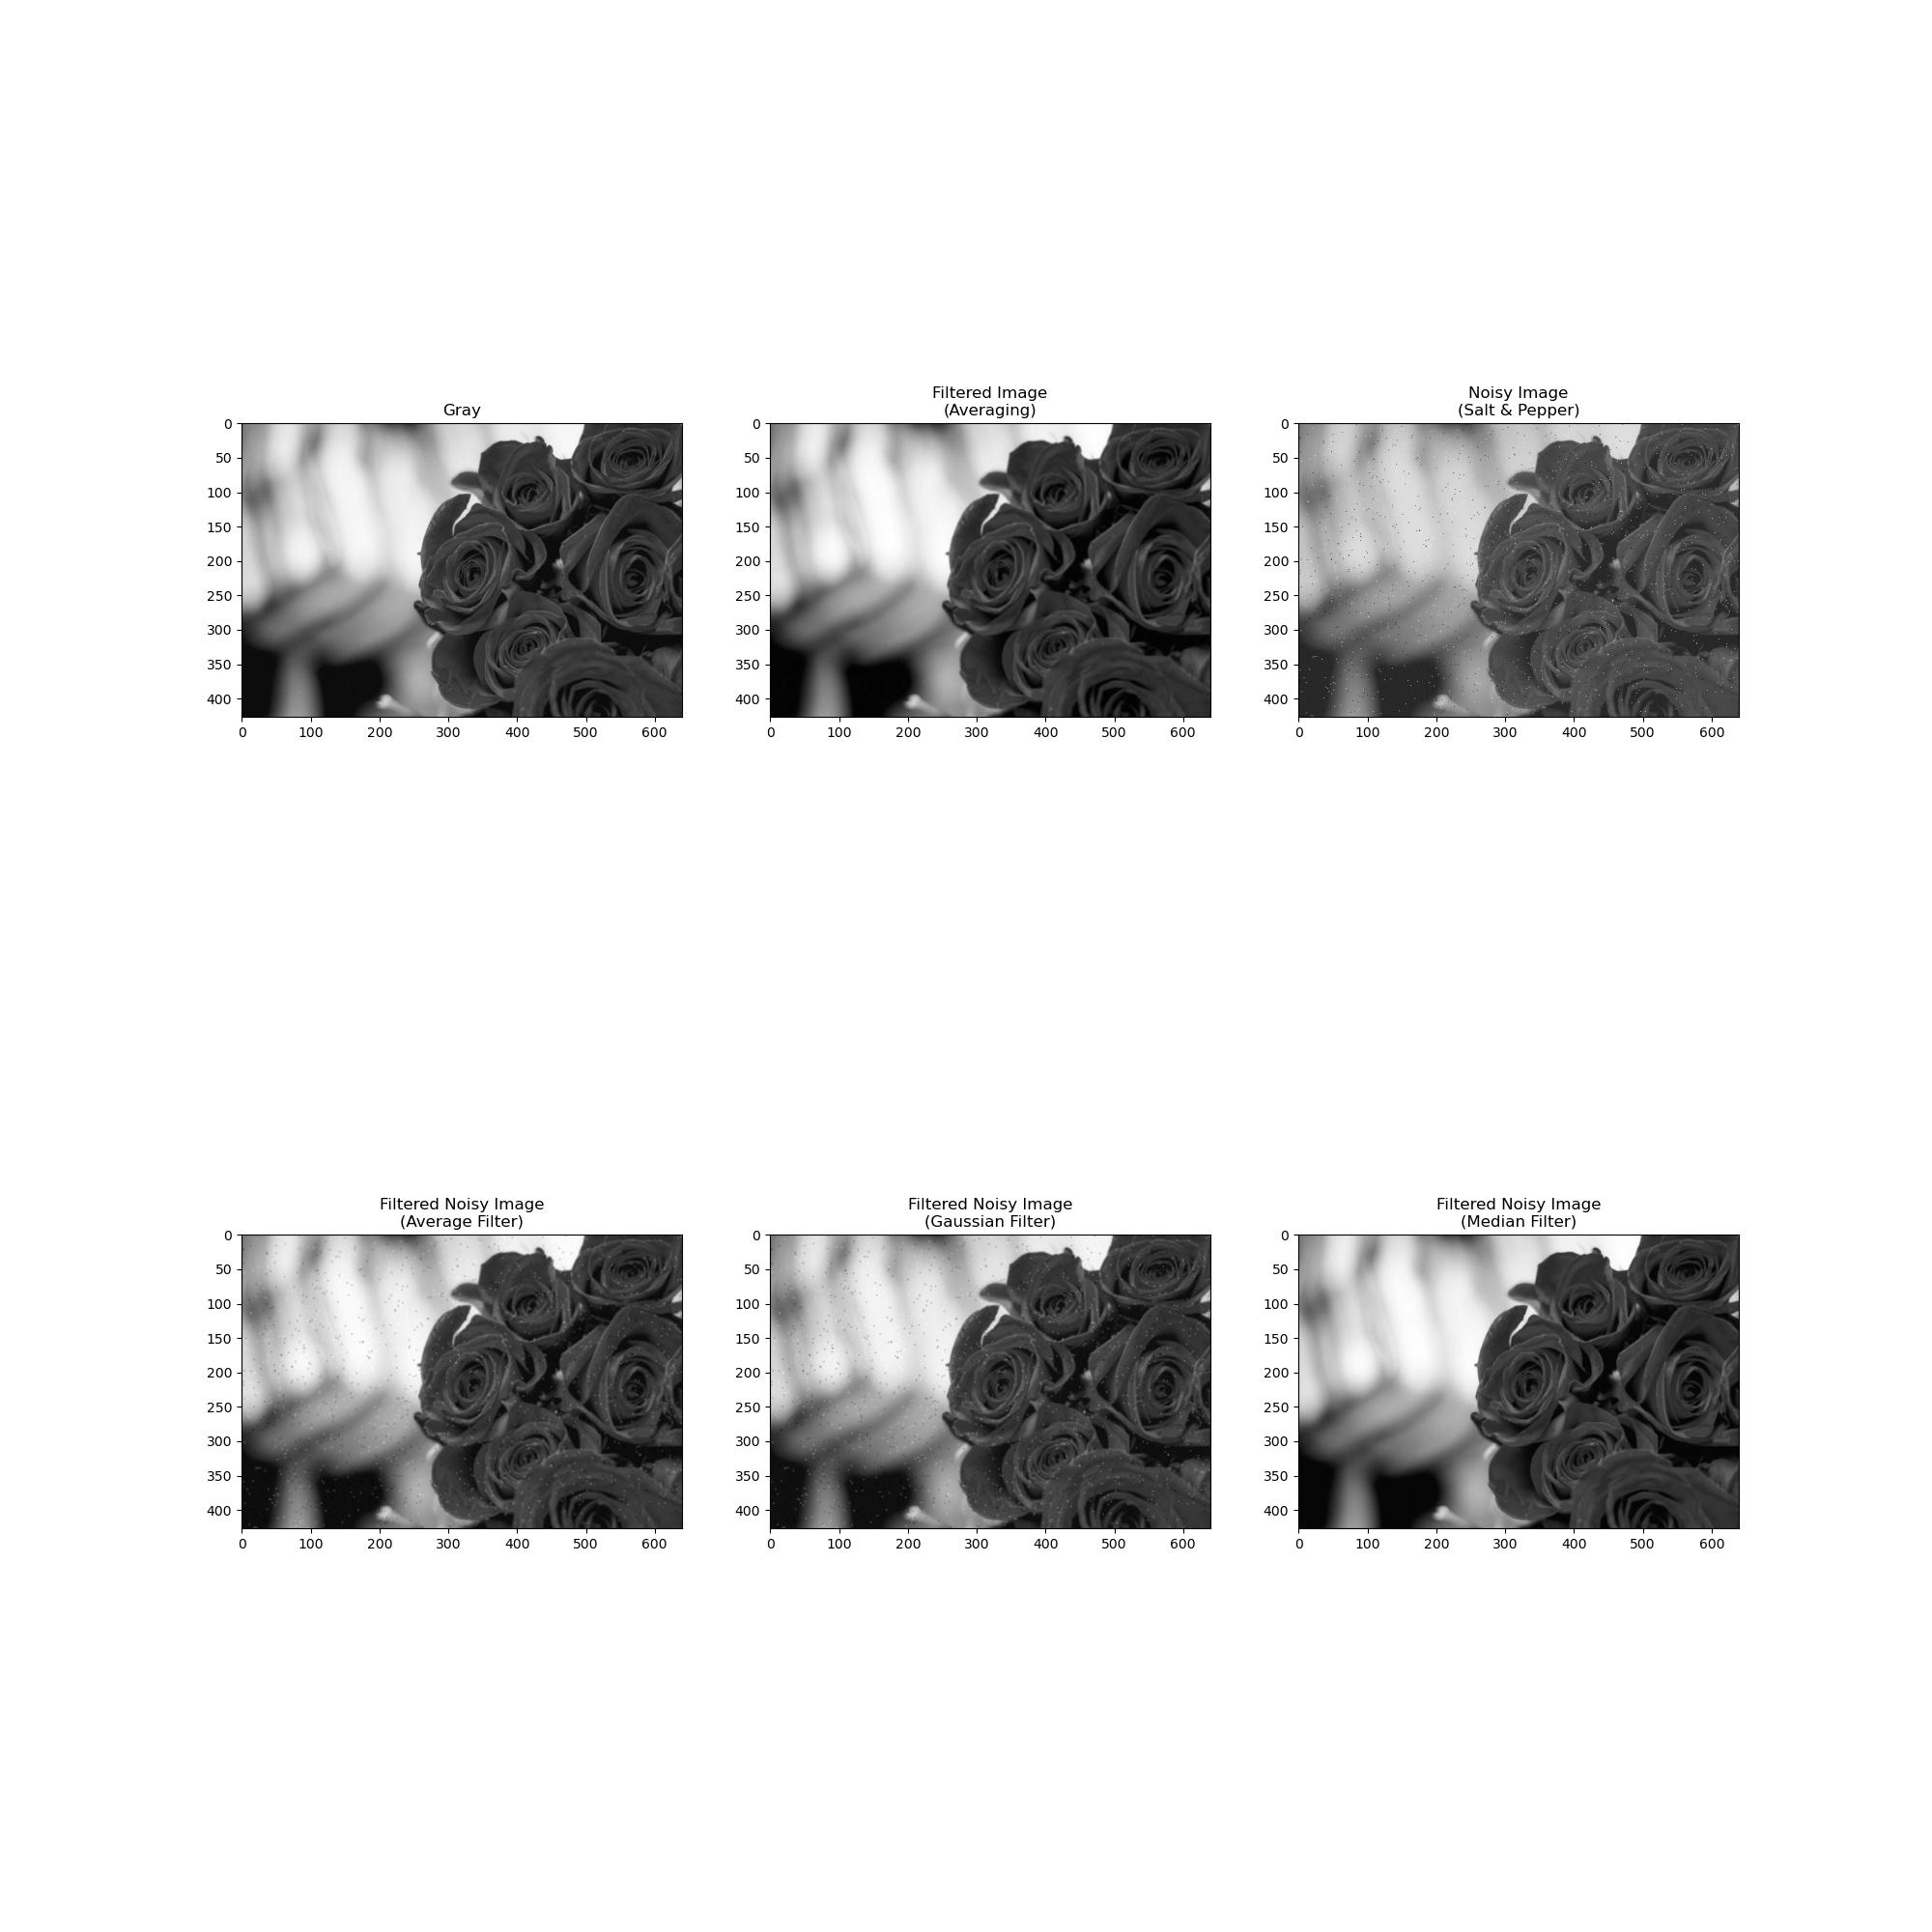
\includegraphics[width=1.0\textwidth]{Assignment-6/noise.jpg}
            \caption{grayscale image; average filtering in gray scale image; adding salt and pepper noise in the image; outputs of performing the average filtering, Gaussian filtering and median filtering}
        \end{figure}
    }
}
% \pagebreak
\clearpage

%-----------------------Assignment-7--------------------------%
{
    \section{Assignment-7}
    \subsection{Introduction}
    \textbf {Problem: }
    Move intensity of a grayscale image left, right and into a specific range and check its effect on histogram. An example output is attached.
    \begin{figure}[htp]
        \centering
        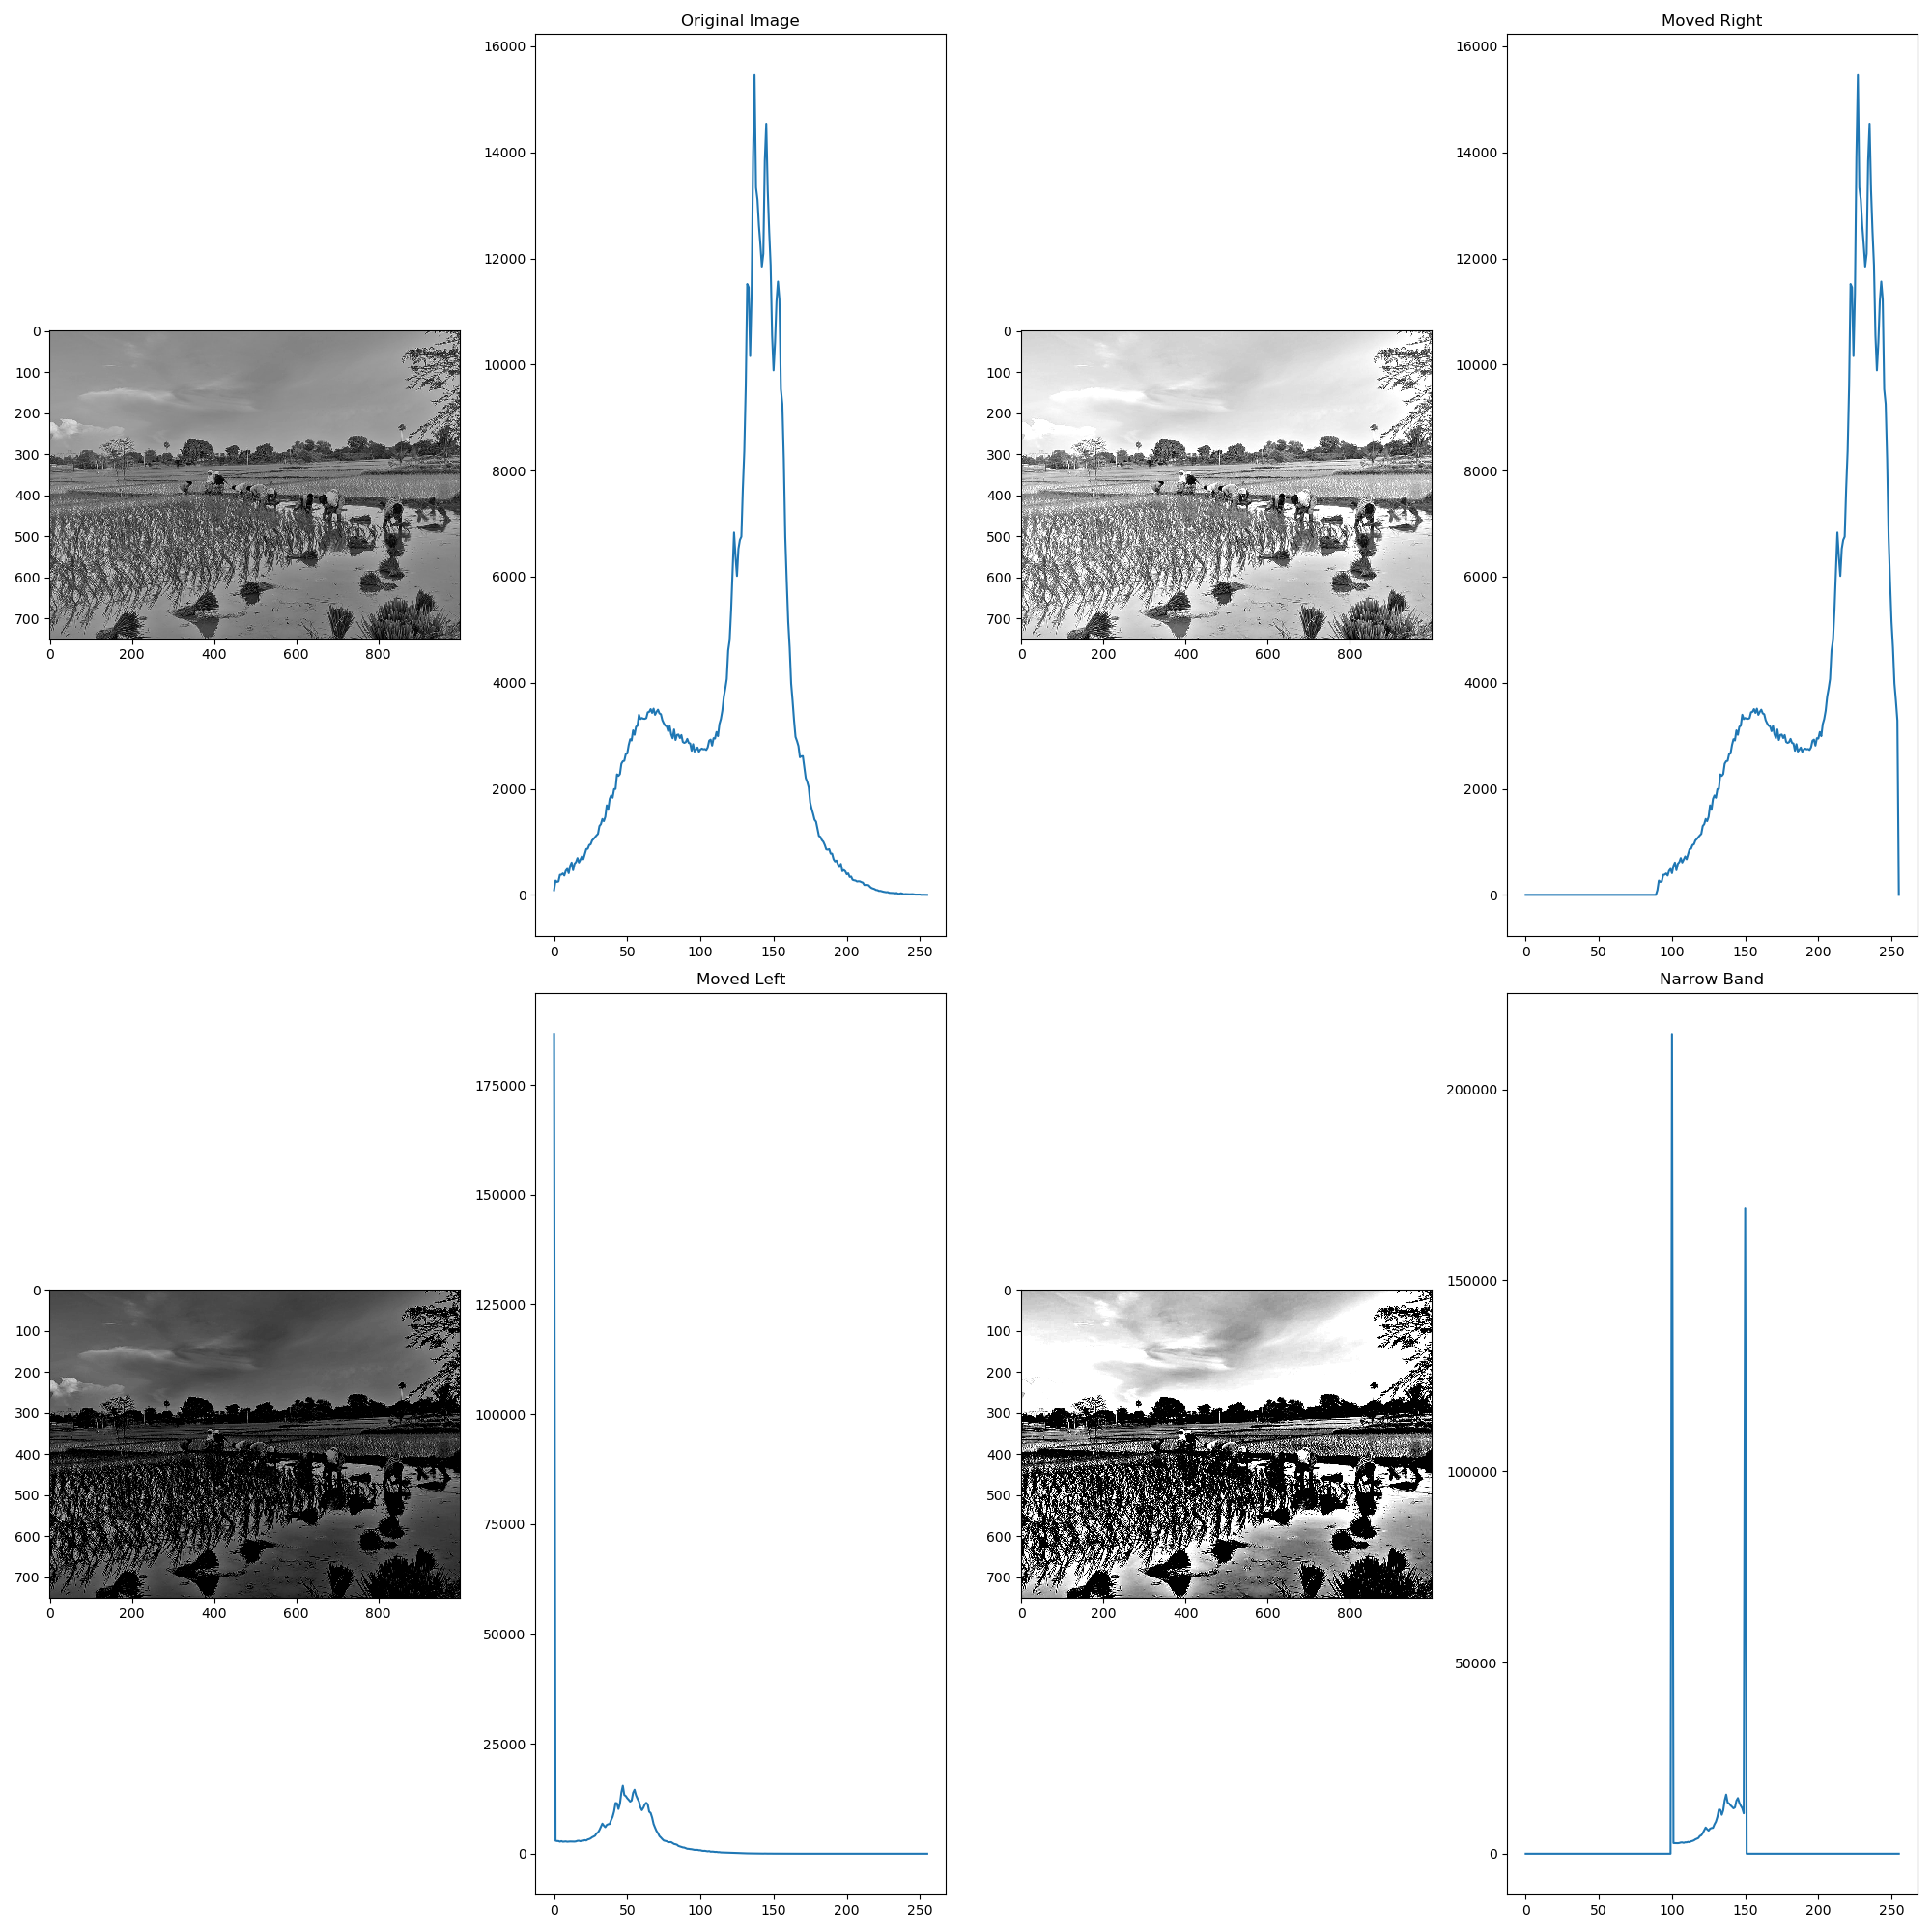
\includegraphics[width=0.55\textwidth]{Assignment-7/PaddyField_Histogram.png}
        \caption{histogram shifting sample}
    \end{figure}
    \\
    \\
    \textbf{Solution: }
    Here, we have to find out the histogram of a grayscale image  at first. Then we have to move the intensity of that image to left, right and to a specific range as given in the picture. To perform the given task, the following program is used.
    \\
    
    \subsection{Required Software}
    For completing this task, we have to install open-cv, matplotlib and numpy. In our programs, we have to import the open-cv(cv2), matplotlib.pyplot as plt and numpy as np. We can install this three libraries using pip3. For different operations open-cv(cv2), numpy and matplotlib will have to be used - specially matplotlib for plotting and saving image. 
    \\
    
    \subsection{Procedure}
    \textbf{Step-1:}
    Install matplotlib, open-cv, numpy libraries.\\
    \textbf{Step-2:}
    Import them in our program. (matplotlib.pyplot as plt, cv2 as cv, numpy as np)\\
    \textbf{Step-3:}
    Read the RGB image and convert it to grayscale using cv.cvtColor() function.\\
    \textbf{Step-4:}
    Perform the given intensity shift operations and save them.\\
    \textbf{Step-5:}
    Find out the histogram of the previously saved images using cv.calcHist() function. Save the outputs.\\
    \textbf{Step-6:}
    Plot all the required images and save them as required in the question.\\
    
    \subsection{Code}
    \lstset{style=mystyle}
    \begin{lstlisting}[language=Python, caption=Code for shifting histogram]
    import matplotlib.pyplot as plt
    import numpy as np
    import cv2 as cv
    
    def main():
        path = './tower.jpg'
        print(path)
    
        rgb = plt.imread(path)
        print(rgb.shape)
    
        grayscale = cv.cvtColor(rgb, cv.COLOR_RGB2GRAY) + 50
        print(grayscale.shape)
    
        img_shift_left = np.copy(grayscale)
        img_shift_right = np.copy(grayscale)
    
        r, c = grayscale.shape
    
        img_shift_left -= 25
        # for i in range(r):
        #     for j in range(c):
        #         img_shift_left[i][j] -= 50
        
        img_shift_right += 25
        # for i in range(r):
        #     for j in range(c):
        #         img_shift_right[i][j] += 50
    
        img_range_check = np.copy(grayscale)
        
        for i in range(r):
            for j in range(c):
                if (img_range_check[i][j] <= 65):
                    img_range_check[i][j] = 65
                elif (img_range_check[i][j] >= 212):
                    img_range_check[i][j] = 212
    
        # print(img_range_check.shape)
        # print(img_range_check)
    
        gray_hist = cv.calcHist([grayscale], [0], None, [256], [0, 256])
        left_hist = cv.calcHist([img_shift_left], [0], None, [256], [0, 256])
        right_hist = cv.calcHist([img_shift_right], [0], None, [256], [0, 256])
        narrow_band_hist = cv.calcHist([img_range_check], [0], None, [256], [0, 256])
    
        img_set = [grayscale, img_shift_left, img_shift_right, img_range_check]
        title_set = ['Gray Image', 'Left shifted image', 'Right shifted image', 'Narrow band image']
        hist_set = [gray_hist, left_hist, right_hist, narrow_band_hist]
    
        plt.figure(figsize = (20, 20))
        j = 0
        for i in range(len(img_set)):
            j += 1
            plt.subplot(2, len(img_set), j)
            plt.title(title_set[i])
            plt.imshow(img_set[i], cmap = 'gray')
    
            plt.subplot(2, len(img_set), j+len(img_set))
            plt.title(title_set[i] + ' histogram')
            plt.plot(hist_set[i])
    
        plt.savefig('fig-1.jpg')
        plt.show()
    
    if __name__ == '__main__':
        main()

    \end{lstlisting}
    \\
    
    \subsection{Result & Discussion}{
        Here, as at first, we read/load the RGB image then convert it to grayscale. Then we shift the intensity of the images and find out the shifted histogram of those images. If we look at the outputs, we can see that, we have got the same output as given in the problem description. As we get the expected output, so it can be said that the task is completed and our program works accurately.
        
        \begin{figure}[htp]
            \centering
            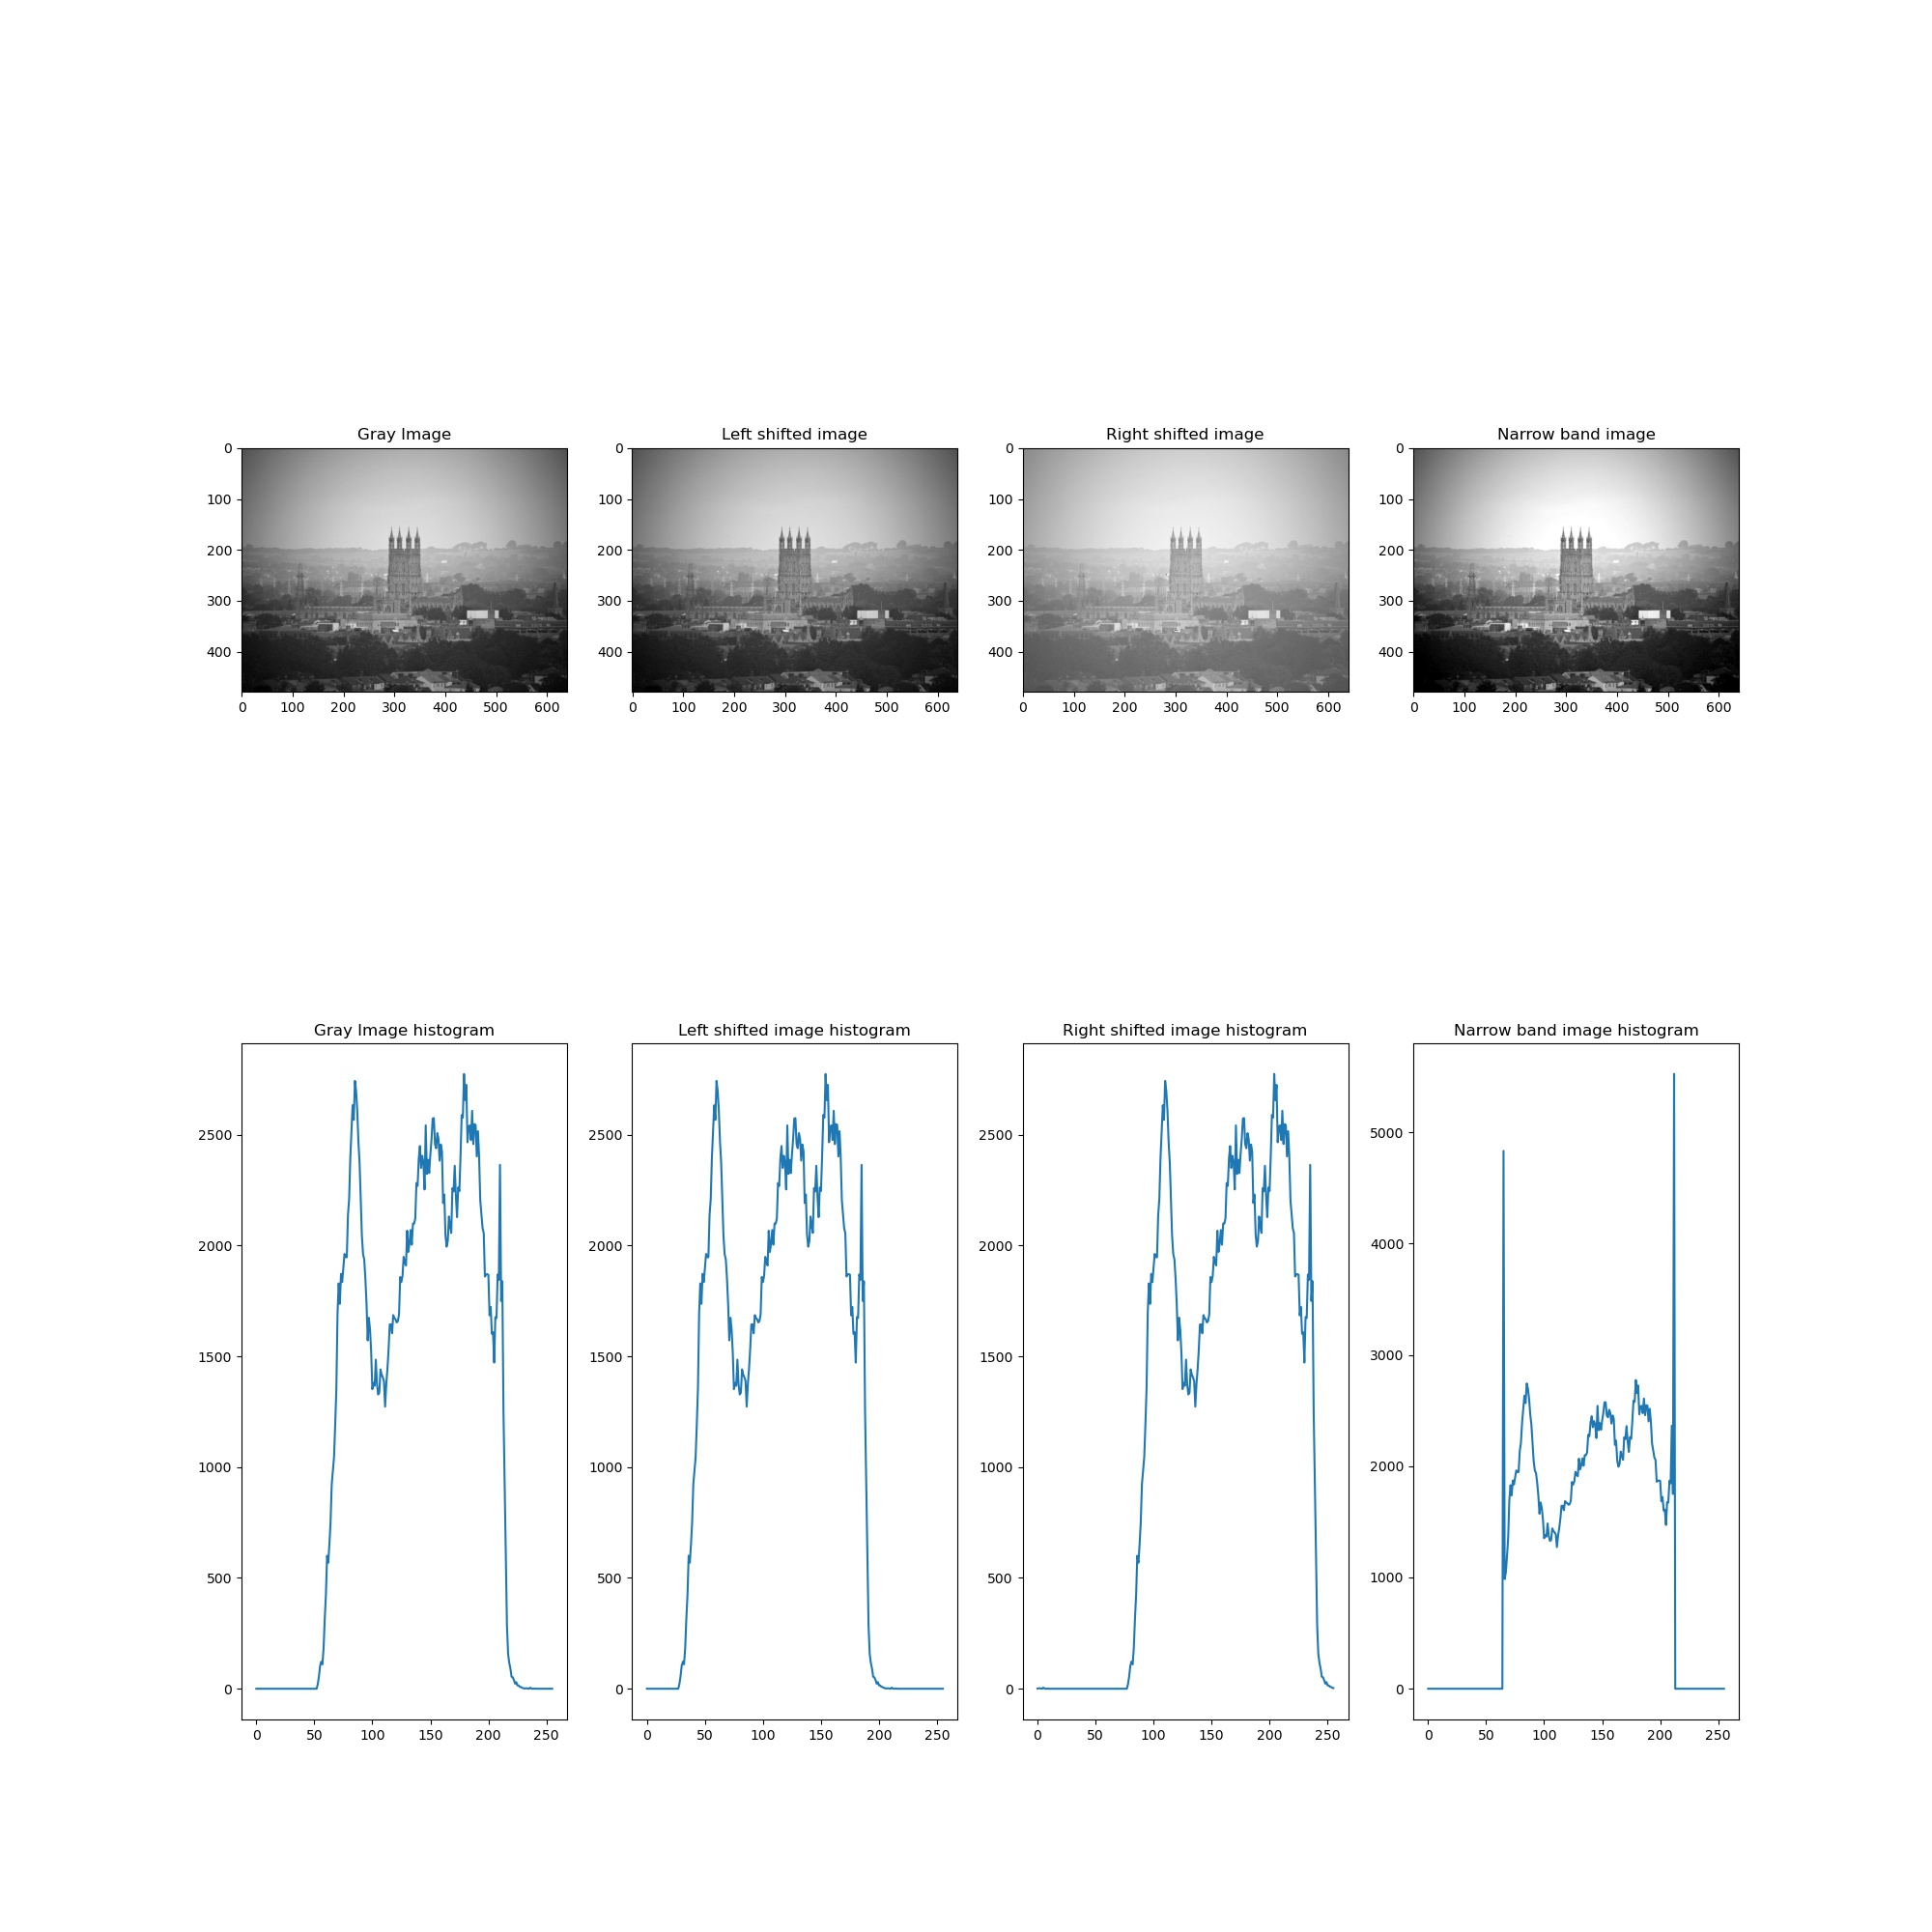
\includegraphics[width=1.0\textwidth]{Assignment-7/fig-1.jpg}
            \caption{grayscale image and its histogram and shifted images and their histogram}
        \end{figure}
    }
}
% \pagebreak
\clearpage

%-----------------------Assignment-8--------------------------%
{
    \section{Assignment-8}
    \subsection{Introduction}
    \textbf {Problem: }
    Explain what happens when you apply morphological dilation, erosion, opening, and closing operations using at least three kinds of structuring elements on your favorite binary image.\\
    ** You can use OpenCV's built -in functions.\\
    ** Using Latex for generating PDF is mandatory.\\
    \\
    \textbf{Solution: }
    Here at first, we have to load a RGB image, convert it to grayscale then again convert it to binary. We have to perform the morphological operation on the images using the built-in function. For doing the morphological operations, we take three different structuring elements (same as kernel/filter) and save the output in three different images. To perform the given task, the following program is used.
    \\
    
    \subsection{Required Software}
    For completing this task, we have to install open-cv, matplotlib and numpy. In our programs, we have to import the open-cv(cv2), matplotlib.pyplot as plt and numpy as np. We can install this three libraries using pip3. For different operations open-cv(cv2), numpy and matplotlib will have to be used - specially matplotlib for plotting and saving image. 
    \\
    
    \subsection{Procedure}
    \textbf{Step-1:}
    Install matplotlib, open-cv, numpy libraries.\\
    \textbf{Step-2:}
    Import them in our program. (matplotlib.pyplot as plt, cv2 as cv, numpy as np)\\
    \textbf{Step-3:}
    Read the RGB image and convert it to grayscale using cv.cvtColor() function. Then convert the grayscale image to binary image using cv.threshold() function.\\
    \textbf{Step-4:}
    Perform the given morphological operations. For erosion use cv.erode() function. For dilation, use cv.dilate() function. For opening and closing use cv.morphologyEx() function. Save the outputs.\\
    \textbf{Step-5:}
    Plot all the required images and save them as required in the question.\\
    
    \subsection{Code}
    \lstset{style=mystyle}
    \begin{lstlisting}[language=Python, caption=Code for performing morphological operations in a binary image]
    import matplotlib.pyplot as plt
    import numpy as np
    import cv2 as cv
    
    def main():
        img_path = "./writing.jpg"
        print(img_path)
    
        img_rgb = plt.imread(img_path)
        print(img_rgb.shape)
    
        img_gray = cv.cvtColor(img_rgb, cv.COLOR_RGB2GRAY)
        print(img_gray.shape)
    
        img_binary = cv.threshold(img_gray, 127, 255, cv.THRESH_BINARY)[1]
        print(img_binary)
    
        kernel1 = np.ones((3, 3))
        kernel2 = np.array([[1, 1, 1],[2, 2, 2], [3, 3, 3]])
        kernel3 = np.array([[3, 3, 3],[2, 2, 2], [1, 1, 1]])
    
        img_erosion1 = cv.erode(img_binary, kernel1, iterations=1)
        img_erosion2 = cv.erode(img_binary, kernel2, iterations=1)
        img_erosion3 = cv.erode(img_binary, kernel3, iterations=1)
    
        img_dilattion1 = cv.dilate(img_binary, kernel1, iterations=1)
        img_dilattion2 = cv.dilate(img_binary, kernel2, iterations=1)
        img_dilattion3 = cv.dilate(img_binary, kernel3, iterations=1)
    
        img_opening1 = cv.morphologyEx(img_binary, cv.MORPH_OPEN, kernel1)
        img_opening2 = cv.morphologyEx(img_binary, cv.MORPH_OPEN, kernel2)
        img_opening3 = cv.morphologyEx(img_binary, cv.MORPH_OPEN, kernel3)
        
        img_closing1 = cv.morphologyEx(img_binary, cv.MORPH_CLOSE, kernel1)
        img_closing2 = cv.morphologyEx(img_binary, cv.MORPH_CLOSE, kernel2)
        img_closing3 = cv.morphologyEx(img_binary, cv.MORPH_CLOSE, kernel3)
    
        img_set1 = [img_rgb, img_gray, img_binary, img_erosion1, img_dilattion1, img_opening1, img_closing1]
        img_set2 = [img_rgb, img_gray, img_binary, img_erosion2, img_dilattion2, img_opening2, img_closing2]
        img_set3 = [img_rgb, img_gray, img_binary, img_erosion3, img_dilattion3, img_opening3, img_opening3]
        img_all = [img_set1, img_set2, img_set3]
        img_title = ['RGB', 'Gray', 'Binary', 'Erosion', 'Dilation', 'Opening', 'Closing']
        
        for i in range(3):
            img_plot(img_all[i], img_title, i+1)
    
    def img_plot(img_set, title_set, cnt):
        
        plt.figure(figsize=(30, 30))
        for i in range(len(img_set)):
            plt.subplot(2, 4, i+1)
            plt.title(title_set[i])
            if (i == 0):
                plt.imshow(img_set[i])
            # elif (i == 1):
            #     plt.imshow(img_set[i], cmap='gray')
            else: 
                plt.imshow(img_set[i], cmap='gray')
        plt.savefig('fig' + str(cnt) + '.jpg')
        plt.show()
    
    if __name__ == "__main__":
        main()

    \end{lstlisting}
    \\
    
    \subsection{Result & Discussion}{
        After using the morphological operation different results are obtained. The result for using erosion, dilation, opening and closing operation is given below as follows. Here three different kernels are used. The result is obtained for all the kernels.\\
        \textbf{Erosion}\\
        In theory, erosion erodes away the boundary of objects. That means if an object is shown in white color and the background color is black, then the white color is eroded and so the object becomes thinner. Now in practical, as the object is shown in black color and the background color is white, the white color is decreased. So, the border of the object becomes thicker as it is in black color.\\
        \textbf{Dilation}\\
        In theory, dilation is opposite to erosion. That means if an object is shown in white color and the background color is black, then the white color is increased and so the object becomes thicker. Now in practical, as the object is shown in black color and the background color is white, the white color is increased. So, the border of the object becomes thinner as it is in black color.\\
        \textbf{Opening}\\
        In theory, opening operation is got using an erosion operation followed by a dilation operation. That means after decreasing the border of the object, then the border is somewhat increased. In practical, as the object is defined in opposite to the conventional way, it is seen that at first the border of the object is increased at first in erosion operation, then for dilation operation the border of the object is decreased.\\
        \textbf{Closing}\\
        In theory, closing operation is got using an dilation operation followed by a erosion operation. That means after increasing the border of the object, then the border is somewhat decreased. In practical, as the object is defined in opposite to the conventional way, it is seen that at first the border of the object is decreased at first in dilation operation, then for erosion operation the border of the object is increased.\\
        
        \begin{figure}[htp]
            \centering
            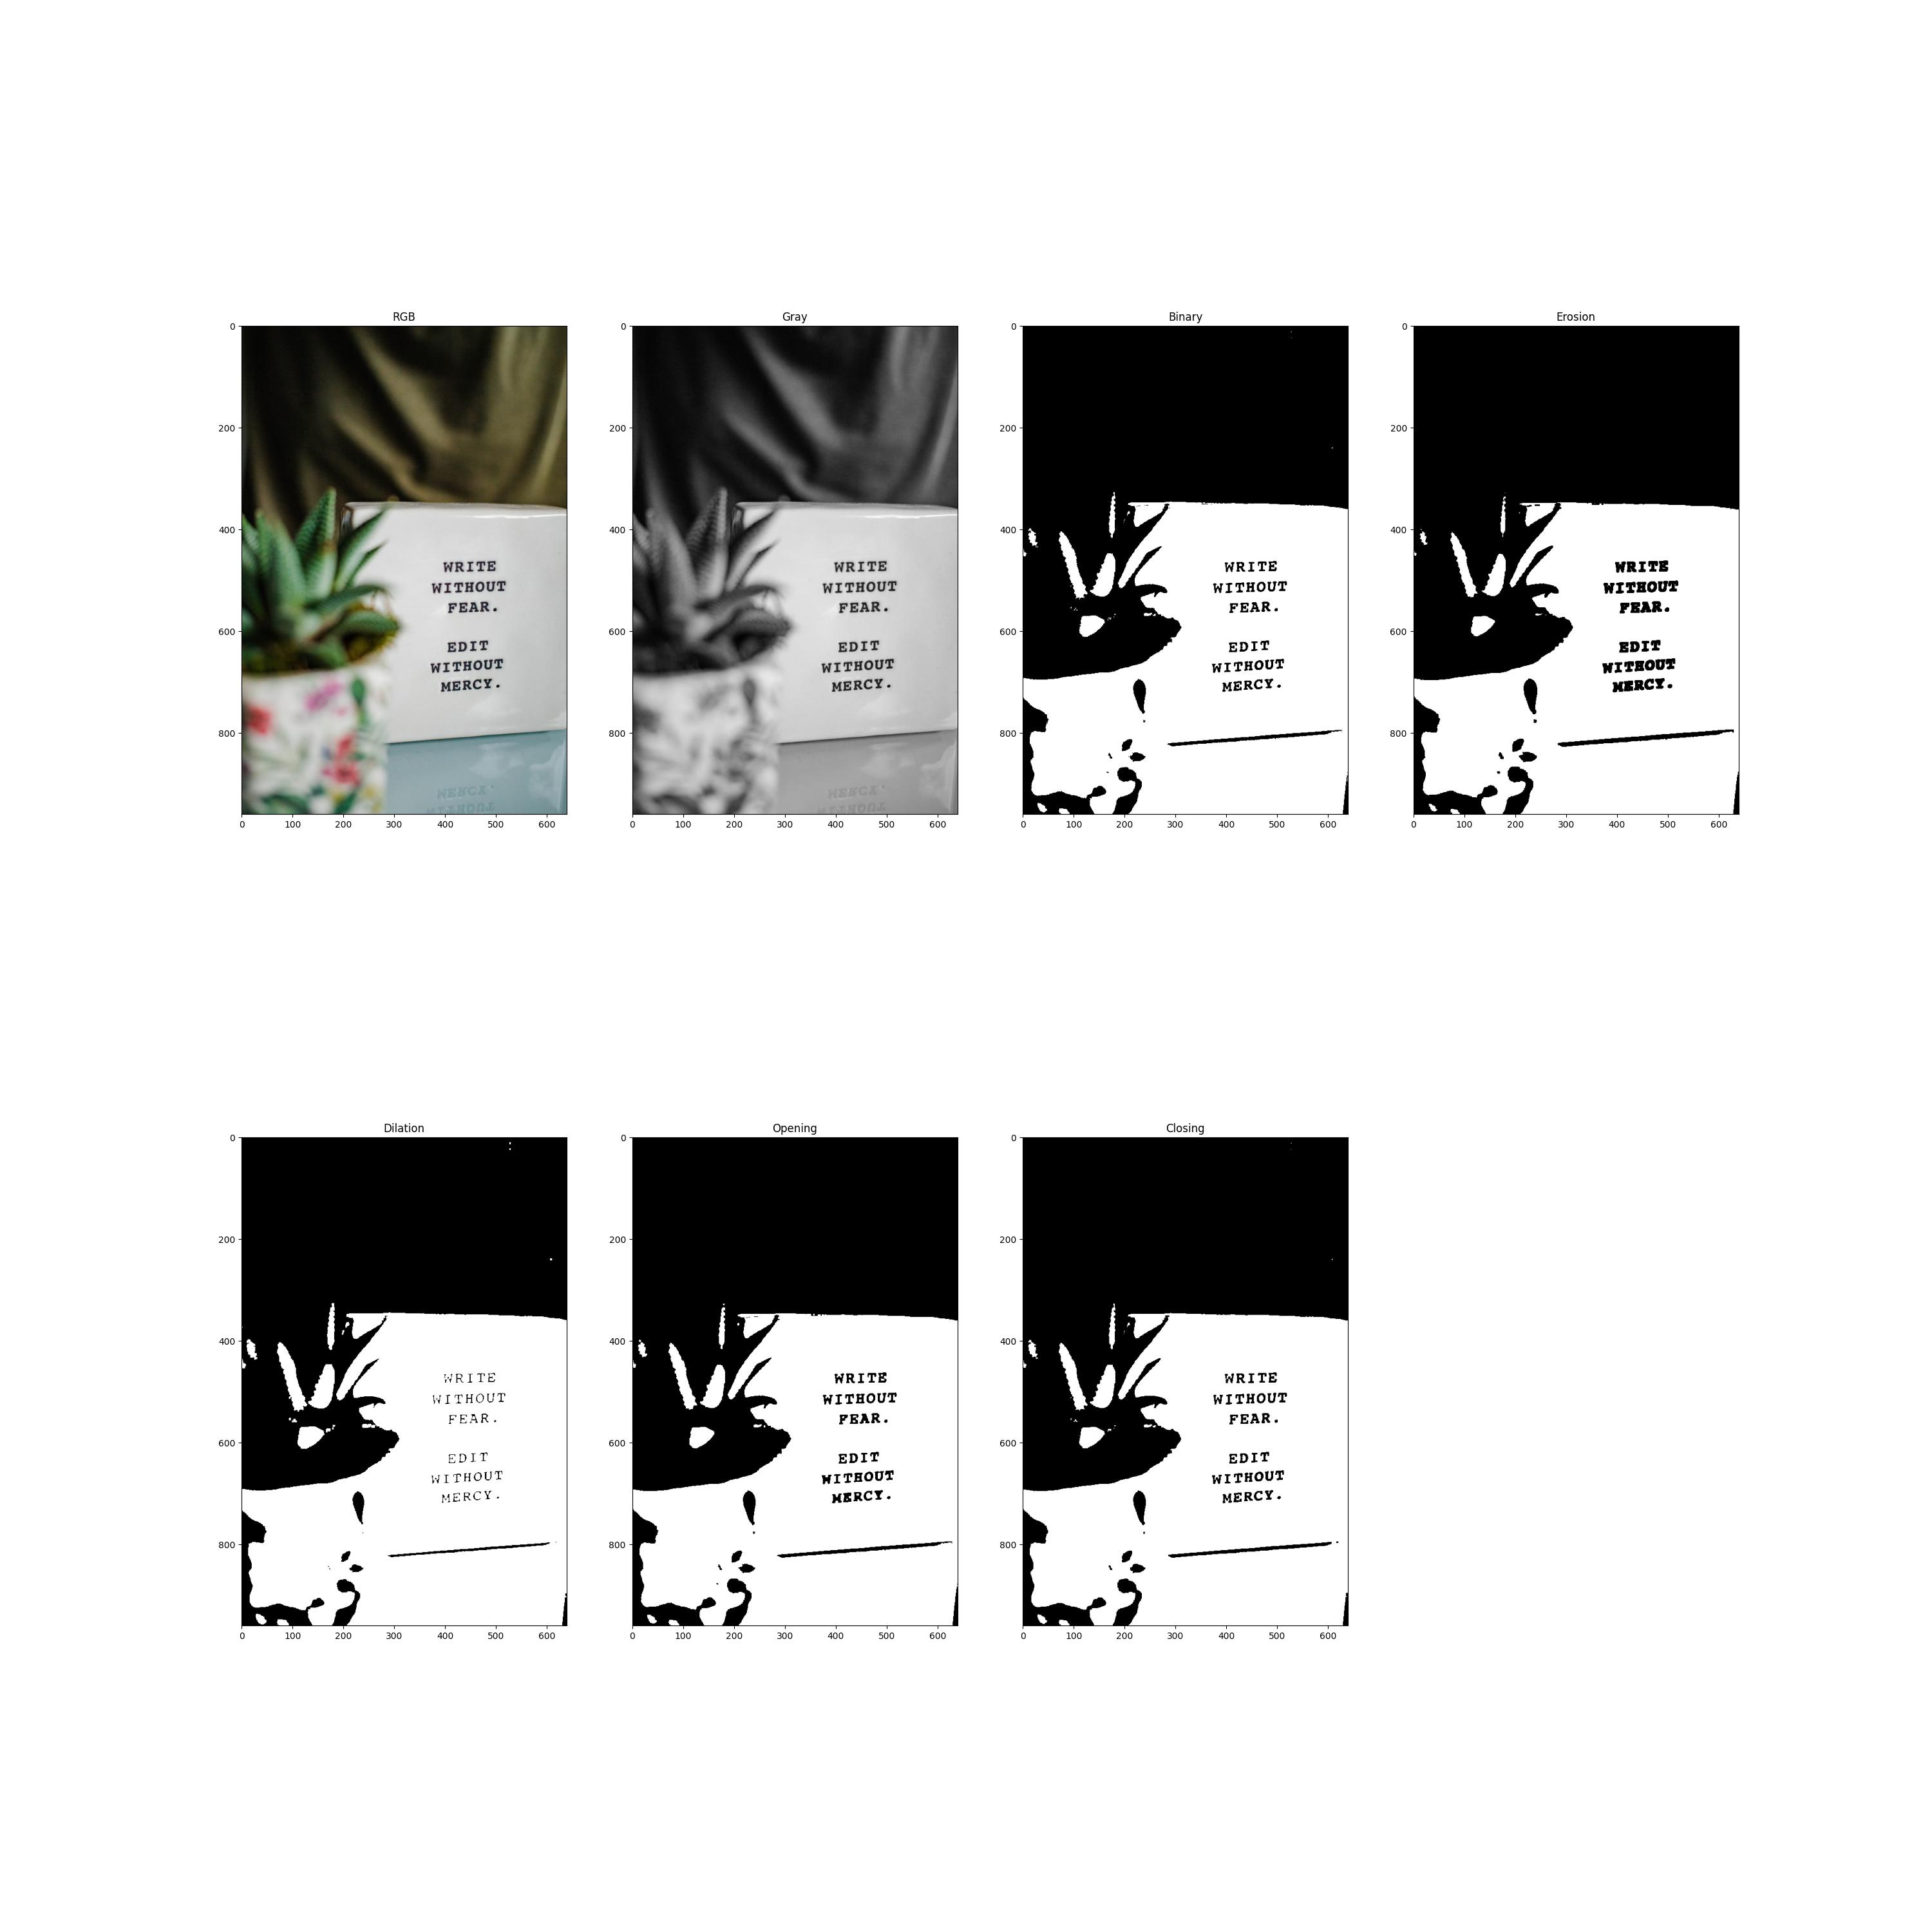
\includegraphics[width=0.49\textwidth]{Assignment-8/fig1.jpg}
            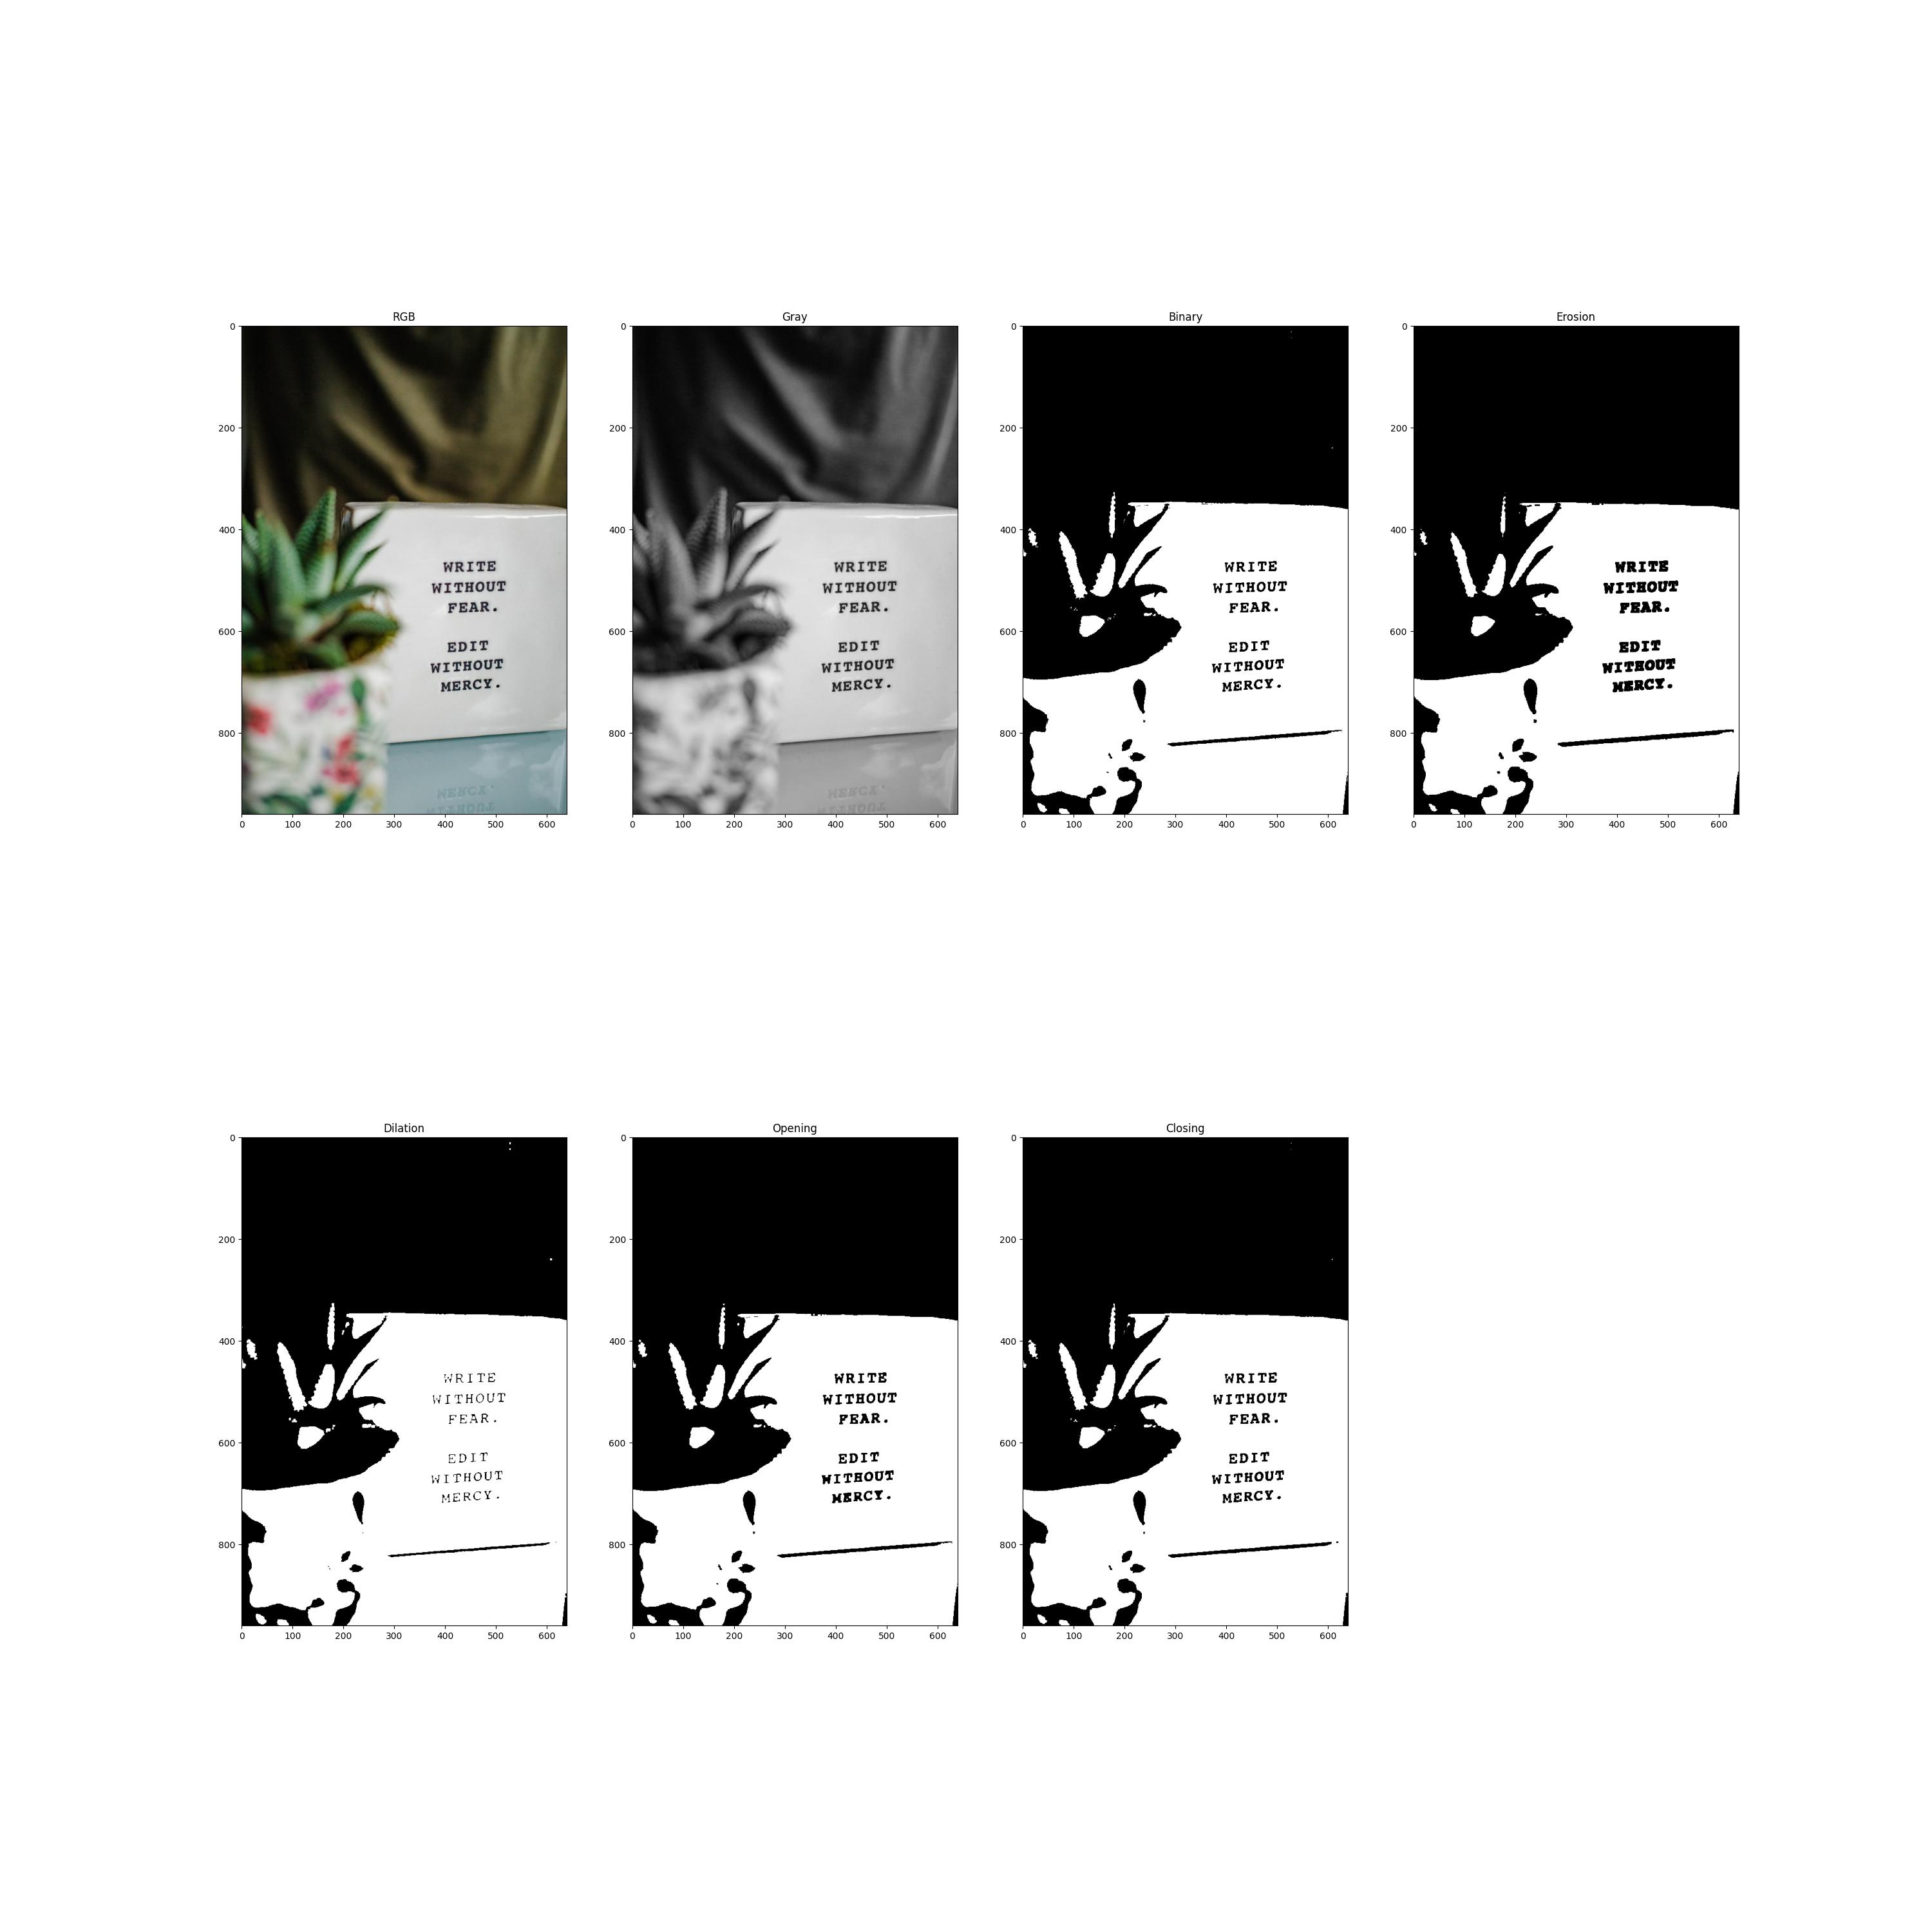
\includegraphics[width=0.49\textwidth]{Assignment-8/fig2.jpg}
            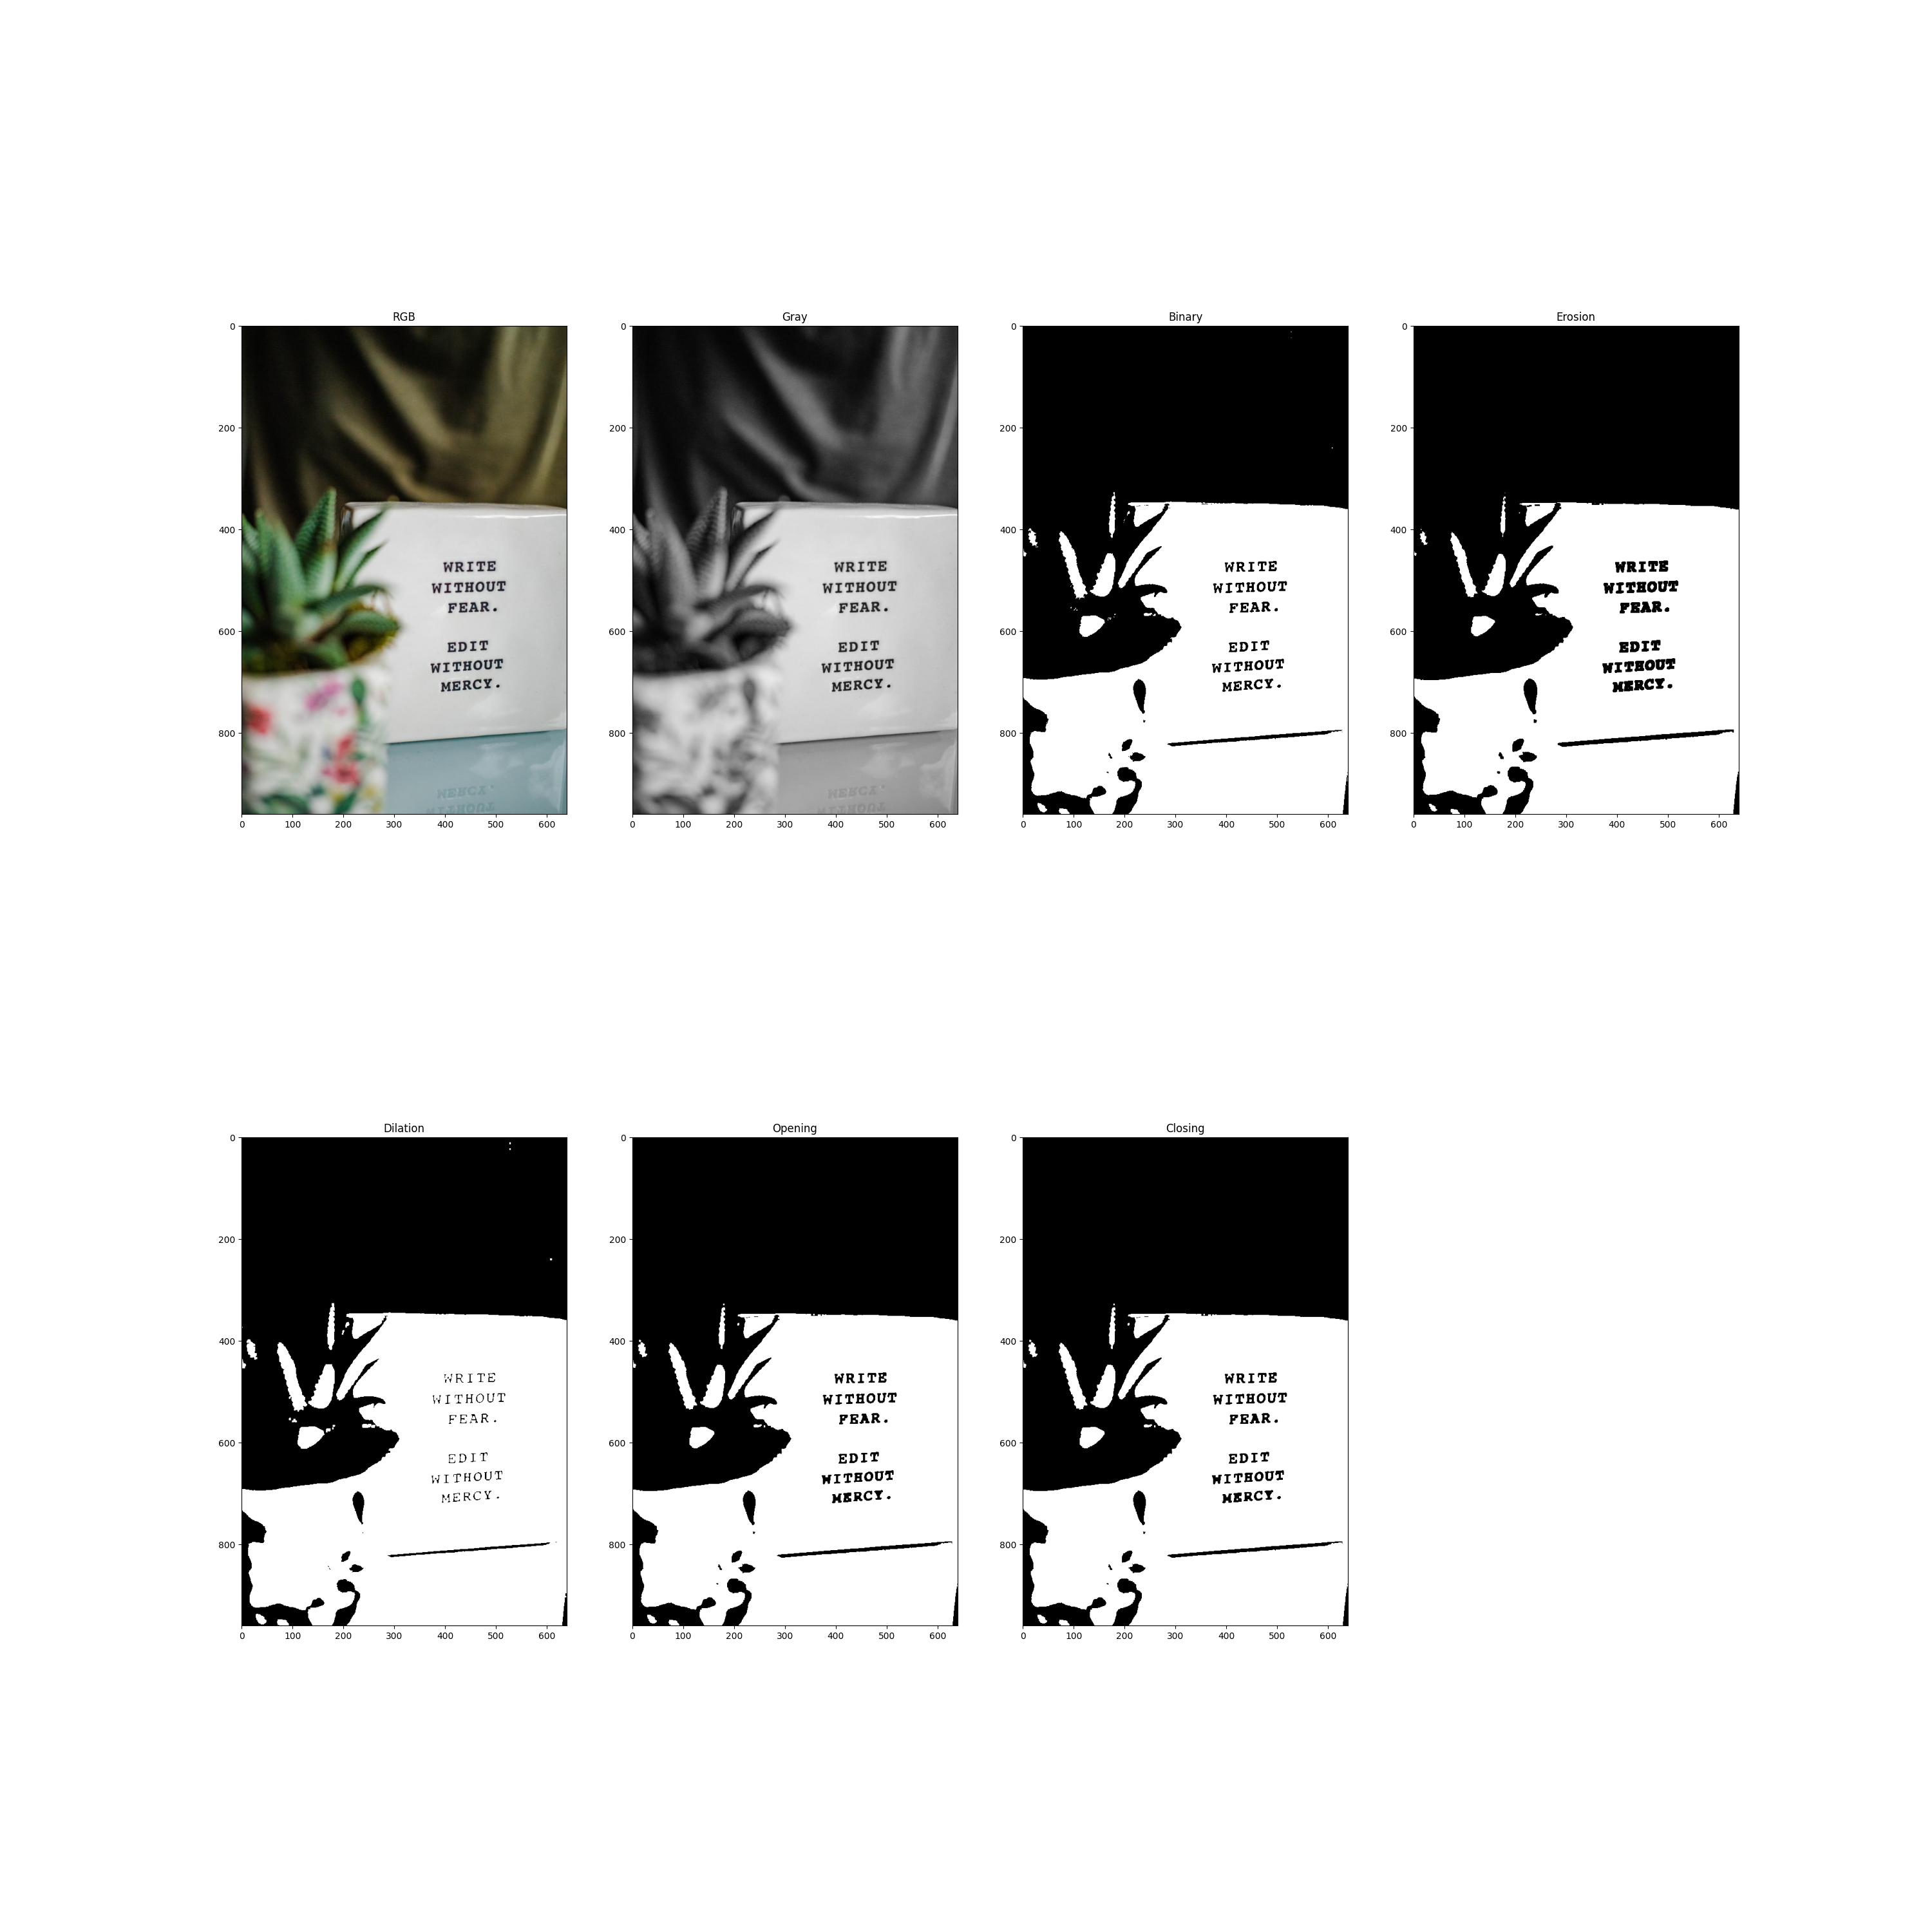
\includegraphics[width=0.5\textwidth]{Assignment-8/fig3.jpg}
            \caption{morphological operations on a for three different structuring elements}
        \end{figure}
    }
}
% \pagebreak
\clearpage

%-----------------------Assignment-9--------------------------%
{
    \section{Assignment-9}
    \subsection{Introduction}
    \textbf {Problem: }
    Implement functions for erosion, dilation, opening and closing operations by Python. Then compare the output of your implemented functions with the output of the OpenCV's built-in functions.\\
    ** Using Latex for generating PDF is mandatory.\\
    \\
    \textbf{Solution: }
    Here at first, we have to load a RGB image, convert it to grayscale then again convert it to binary. We have to perform the morphological operation on the image. Now we have to implement functions for erosion, dilation, opening and closing operation where the parameters of the functions are the image and the structuring element. For erosion and dilation, we use fit and hit concept for calculation. As the opening and closing operation can be implemented using the erosion and dilation operation, we do not create a separate function here - just call the erosion and dilation function sequentially. Then we compare the outputs of the operations using buit-in function and implemented function. To perform the given task, the following program is used.
    \\
    
    \subsection{Required Software}
    For completing this task, we have to install open-cv, matplotlib and numpy. In our programs, we have to import the open-cv(cv2), matplotlib.pyplot as plt and numpy as np. We can install this three libraries using pip3. For different operations open-cv(cv2), numpy and matplotlib will have to be used - specially matplotlib for plotting and saving image. 
    \\
    
    \subsection{Procedure}
    \textbf{Step-1:}
    Install matplotlib, open-cv, numpy libraries.\\
    \textbf{Step-2:}
    Import them in our program. (matplotlib.pyplot as plt, cv2 as cv, numpy as np)\\
    \textbf{Step-3:}
    Read the RGB image and convert it to grayscale directly using the cv.read() function. Then convert the grayscale image to binary image using cv.threshold() function.\\
    \textbf{Step-4:}
    Implement the erosion and dilation function using the concept of hit and fit. For opening operation, do the erosion operation first then dilation operation. For closing operation, perform the same operation as opening but in reverse order.\\
    \textbf{Step-5:}
    Perform the morphological operations on a same image both for built-in function and implemented function and save the outputs.\\
    \textbf{Step-6:}
    Plot all the required images and save them as required in the question.\\
    
    \subsection{Code}
    \lstset{style=mystyle}
    \begin{lstlisting}[language=Python, caption=Code for implementing different morphological operations as functions for a binary image]
    import matplotlib.pyplot as plt
    import numpy as np 
    import cv2 as cv
    
    def main():
        img_path = './board-writing.jpg'
        img_gray = cv.imread(img_path, 0)
        
        # img_rgb = plt.imread(img_path)
        # print(img_rgb.shape)
    
        # img_gray = cv.cvtColor(img_rgb, cv.COLOR_RGB2GRAY)
        print(img_gray.shape)
    
        img_binary = cv.threshold(img_gray, 127, 255, cv.THRESH_BINARY)[1]
        print(img_binary)
    
        kernel = np.ones((3, 3), dtype=np.uint8) 
    
        img_erosion1 = cv.erode(img_binary, kernel, iterations=1)
        img_erosion2 = erosion(img_binary, kernel)
    
        img_dilattion1 = cv.dilate(img_binary, kernel, iterations=1)
        img_dilattion2 = dilation(img_binary, kernel)
    
        img_opening1 = cv.morphologyEx(img_binary, cv.MORPH_OPEN, kernel)
        img_opening2 = dilation(erosion(img_binary, kernel), kernel)
    
        img_closing1 = cv.morphologyEx(img_binary, cv.MORPH_CLOSE, kernel)
        img_closing2 = erosion(dilation(img_binary, kernel), kernel)
    
        img_set = [ img_gray, img_binary, img_erosion1, img_erosion2, img_dilattion1, img_dilattion2, img_opening1, img_opening2, img_closing1, img_closing2]
        img_title = ['Grayscale', 'Binary', 'Erosion 1',  'Erosion 2', 'Dilation 1', 'Dilation 2', 'Opening 1', 'Opening 2', 'Closing 1', 'Closing 2']
        img_plot(img_set, img_title)
    
    def img_plot(img, title):
        plt.figure(figsize=(15, 15))
        j = 0
        for i in range(int(len(img)/2)):
            plt.subplot(2, 5, i+1)
            plt.title(title[j])
            plt.imshow(img[j], cmap = 'gray')
            
            plt.subplot(2, 5, i+5+1)
            plt.title(title[j+1])
            plt.imshow(img[j+1], cmap = 'gray')
            j += 2
    
        plt.savefig('fig-1.jpg')
        plt.show()
    
    def erosion(img_binary, kernel):
        r, c = img_binary.shape
        x, y = kernel.shape
        img_process = np.zeros((r-x-1, c-y-1))
        for i in range(r-x-1):
            for j in range(c-y-1):
                sum = np.sum(img_binary[i:i+x, j:j+y] * kernel) # only for fit, the pixel value will be 1
                check = np.sum(kernel * (255 * np.ones((3, 3))))
                if (sum == check):
                    img_process[i][j] = 255
        return img_process
    
    def dilation(img_binary, kernel):
        r, c = img_binary.shape
        x, y = kernel.shape
        img_process = np.zeros((r-x+1, c-y+1))
        for i in range(r-x+1):
            for j in range(c-y+1):
                sum = np.sum(img_binary[i:i+x, j:j+y] * kernel) 
                if (sum >= 255): # both for fit, hit the pixel value will be 1
                    img_process[i][j] = 255
        return img_process
    
    if __name__ == '__main__':
        main()

    \end{lstlisting}
    \\
    
    \subsection{Result & Discussion}{
        As we do different morphological operations on a binary image, we convert the RGB image to grayscale and then to binary. Therefore the first step is done accurately. Then we implement the morphological operations as different functions and obtain the output of them and compare it with the built-in function. The comparison picture is given as follows. Now if we look at the following picture, we can see that the outputs of the built-in functions and implemented functions works almost same. Only the some difference is in detailing. As we get the expected output, so it can be said that the task is completed and our program works accurately.
        
        \begin{figure}[htp]
            \centering
            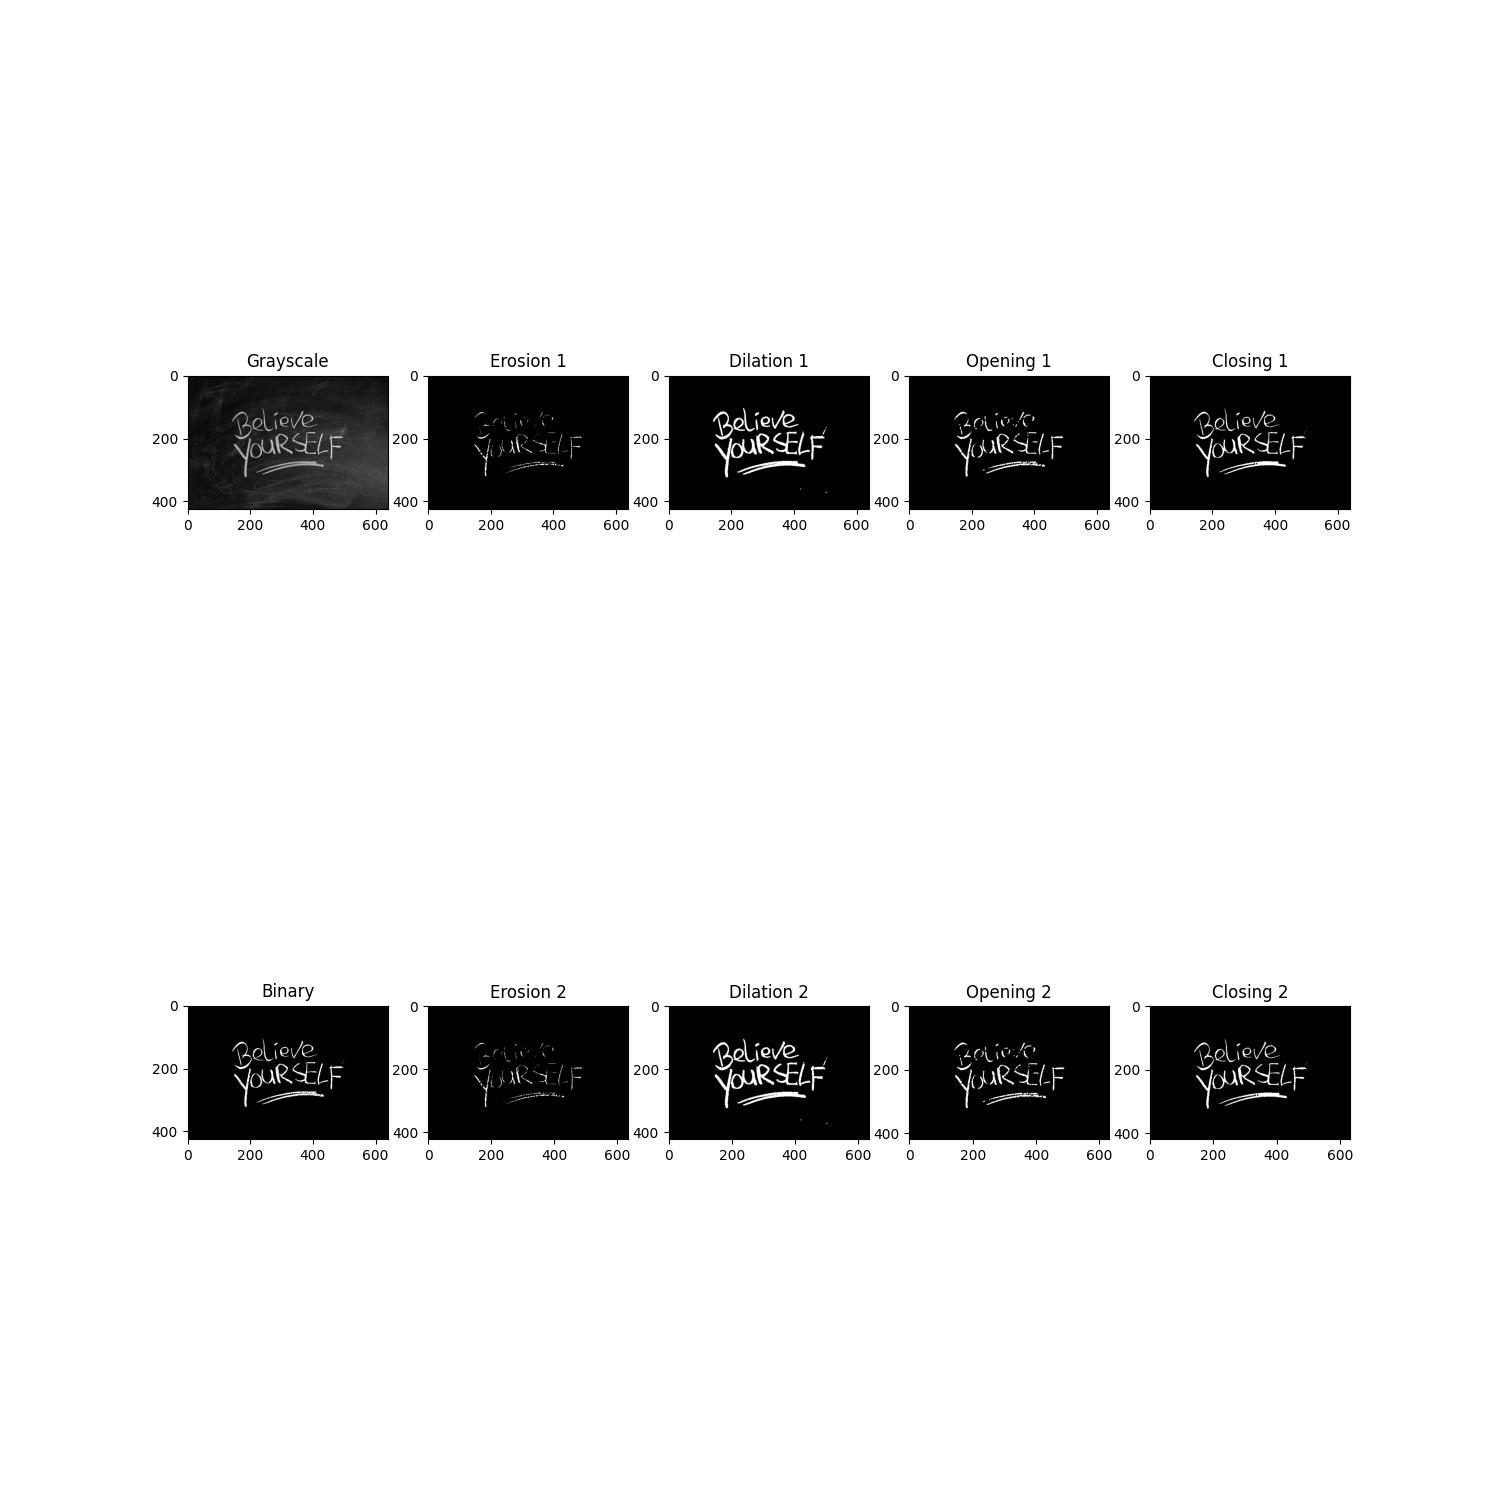
\includegraphics[width=1.0\textwidth]{Assignment-9/fig-1.jpg}
            \caption{morphological operations on a for three different structuring elements}
        \end{figure}
    }
}
% \pagebreak
\clearpage

%-----------------------Assignment-10-------------------------%
{
    \section{Assignment-10}
    \subsection{Introduction}
    \textbf {Problem: }
    What happens when you apply histogram equalization on your favorite grayscale image?\\
    ** Using Latex for generating PDF is mandatory.\\
    \\
    \textbf{Solution: }
    Here at first, we have to load a RGB image, convert it to grayscale. Here, it is better to take a low contrast image for getting better output and showing them. The approaches of solving this task is, we at first, find out the histogram of the image. Then equalize the histogram and again find out the histogram of the equalized image for comparing the histogram. We also want to implement the histogram equalization function and compare the output with the built-in function. In our implementing function, we have to find out the frequencies of the image, probability of the frequencies, cumulative probability of the frequencies, create new pixels and assign them into the corresponding pixels. To perform the given task, the following program is used.
    \\
    
    \subsection{Required Software}
    For completing this task, we have to install open-cv, matplotlib and numpy. In our programs, we have to import the open-cv(cv2), matplotlib.pyplot as plt and numpy as np. We can install this three libraries using pip3. For different operations open-cv(cv2), numpy and matplotlib will have to be used - specially matplotlib for plotting and saving image. 
    \\
    
    \subsection{Procedure}
    \textbf{Step-1:}
    Install matplotlib, open-cv, numpy libraries.\\
    \textbf{Step-2:}
    Import them in our program. (matplotlib.pyplot as plt, cv2 as cv, numpy as np)\\
    \textbf{Step-3:}
    Read the RGB image and convert it directly to grayscale using cv.read() function. Save two copies of the image.\\
    \textbf{Step-4:}
    Find out the histograms of the images and save them.\\
    \textbf{Step-5:}
    Implement the histogram equalize function where calculation of the frequencies of the image, probability of the frequencies, cumulative probability of the frequencies, creating new pixels and assigning them into the corresponding pixels should be done.\\
    \textbf{Step-6:}
    Perform histogram equalization using built-in function and the implemented function. Save the outputs.\\
    \textbf{Step-7:}
    Again find out the histograms of the equalized images and save them.\\
    \textbf{Step-8:}
    Plot all the required images and save them as required in the question.\\
    
    \subsection{Code}
    \lstset{style=mystyle}
    \begin{lstlisting}[language=Python, caption=Code for histogram equalization]
    import matplotlib.pyplot as plt
    import numpy as np
    import cv2 as cv
    
    def main():
        img_path = './tower.jpg'
        img_gray = cv.imread(img_path, 0)
        print(img_gray.shape)
    
        img1 = np.copy(img_gray)
        img2 = np.copy(img_gray)
    
        hist = cv.calcHist(img1, [0], None, [256], [0, 256])
        
        img_hist_equalized1 = cv.equalizeHist(img1)
        new_hist1 = cv.calcHist(img_hist_equalized1, [0], None, [256], [0, 256]) 
    
        img_hist_equalized2 = equalizeHistogram(img2)
        # print(img_hist_equalized2.shape)
        # print(img_hist_equalized2)
        new_hist2 = cv.calcHist(img_hist_equalized2, [0], None, [256], [0, 256])
    
        set1 = [img1, hist, img_hist_equalized1, new_hist1]
        set2 = [img2, hist, img_hist_equalized2, new_hist2]
        title = ['Original\nImage', 'Original\nHistogram', 'Equalized\nImage', 'Equalized\nHistogram']
    
        plt.figure(figsize=(15, 15))
        for i in range(len(set1)):
            plt.subplot(2, 4, i+1)
            plt.title(title[i])
            if (i % 2 == 0):
                plt.imshow(set1[i], cmap='gray')
            else: 
                plt.plot(set1[i])
    
            plt.subplot(2, 4, i+1+4)
            plt.title(title[i])
            if (i % 2 == 0):
                plt.imshow(set2[i], cmap='gray')
            else: 
                plt.plot(set2[i])
        
        plt.savefig('fig-1.jpg')
        plt.show()
    
    def equalizeHistogram(img_old):
        
        r, c = img_old.shape 
        frequency = np.arange(0, 256)
        frequency[:] = 0
    
        # frequency count
        for i in range(r):
            for j in range(c):
                frequency[img_old[i][j]] += 1
        
        # total no of frequency
        total = r*c
        
        # probability of the frequencies
        pdf = []
        for i in range(256):
            pdf.append(frequency[i]/total)
        
        # probability of cumulative frequencies
        cdf = []
        cf = 0
        for i in range(256):
            cf += frequency[i]
            cdf.append(cf/total)
        
        # new pixel values
        new_pixel = np.arange(0, 256)
        for i in range(256):
            new_pixel[i] = round(cdf[i] * 255)
    
        # assigning new values to new image (equalized image)
        img_new = np.zeros((r, c), dtype=np.uint8)
        for i in range(r):
            for j in range(c):
                img_new[i][j] = new_pixel[img_old[i][j]]
    
        return img_new
    
    if __name__ == '__main__':
        main()

    \end{lstlisting}
    \\
    
    \subsection{Result & Discussion}{
        As we are performing histogram equalization, at first low contrast image is taken. The histogram of this image is obtained. Then we perform histogram equalization using the built-in function and implemented function and obtained the outputs. All the outputs are shown as follows. Now if we look at the following picture, we can see that the outputs of the built-in functions and implemented functions are same. As we get the expected output, so it can be said that the task is completed and our program works accurately.
        
        \begin{figure}[htp]
            \centering
            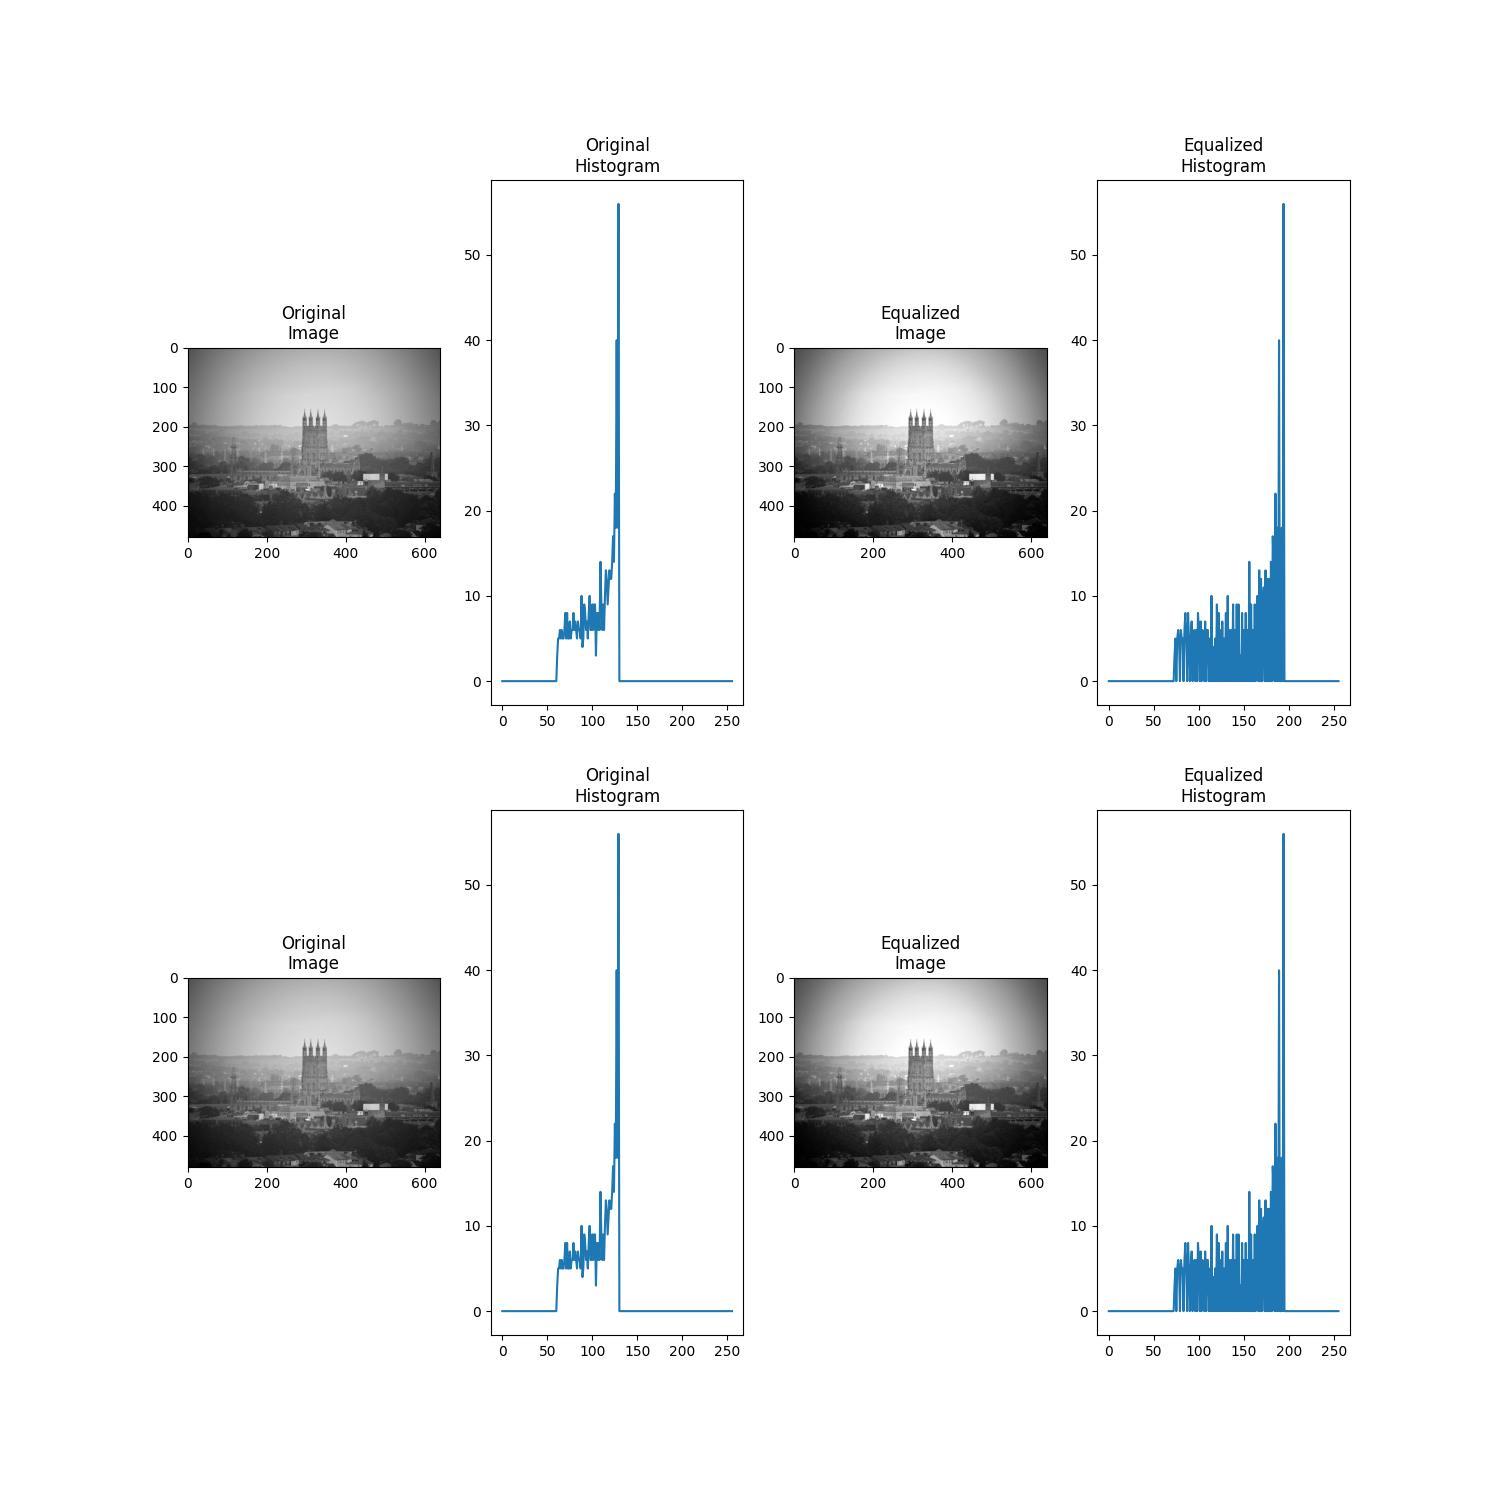
\includegraphics[width=0.9\textwidth]{Assignment-10/fig-1.jpg}
            \caption{Outputs of histogram equalization}
        \end{figure}
    }
}
% \pagebreak
\clearpage

%-----------------------Assignment-11-------------------------%
{
    \section{Assignment-11}
    \subsection{Introduction}
    \textbf {Problem: }
    Explain what happens when you apply filtering in frequency domain. Try at least 4 different filters. You can take help from the attached code.\\
    \\
    \textbf{Solution: }
    Here at first, we have to load a RGB image, convert it to grayscale. Then we have to create some filters. Here we have created ideal low pass filter, ideal high pass filter, Gaussian low pass filter, Gaussian high pass filter, Butterworth low pass filter and Butterworth high pass filter. After that, we have to perform the Fourier transform the image and perform AND operation with the filters for filtering. At last for obtaining the output, we have again perform inverse Fourier transform. For doing these, the following program is used.
    \\
    
    \subsection{Required Software}
    For completing this task, we have to install open-cv, matplotlib and numpy. In our programs, we have to import the open-cv(cv2), matplotlib.pyplot as plt and numpy as np. We can install this three libraries using pip3. For different operations open-cv(cv2), numpy and matplotlib will have to be used - specially matplotlib for plotting and saving image. 
    \\
    
    \subsection{Procedure}
    \textbf{Step-1:}
    Install matplotlib, open-cv, numpy libraries.\\
    \textbf{Step-2:}
    Import them in our program. (matplotlib.pyplot as plt, cv2 as cv, numpy as np)\\
    \textbf{Step-3:}
    Read the RGB image and convert it to grayscale using cv.cvtColor() function and save it.\\
    \textbf{Step-4:}
    Create ideal low pass filter, ideal high pass filter, Gaussian low pass filter, Gaussian high pass filter, butterworth low pass filter and butterworth high pass filter. Create just one of the filers from the pair and get the other one by subtracting the previous filter from 1.\\
    \textbf{Step-5:}
    Perform Fourier transform of the image and for magnitude spectrum, multiply it with logarithmic function.\\
    \textbf{Step-6:}
    Perform filtering operation by multiplying the transform image with the filters.\\
    \textbf{Step-7:}
    Again perform inverse Fourier transform for getting the expected output and save them.\\
    \textbf{Step-8:}
    Plot all the required images and save them as required in the question.\\
    
    \subsection{Code}
    \lstset{style=mystyle}
    \begin{lstlisting}[language=Python, caption=Code for applying filters in frequency domain]
    import matplotlib.pyplot as plt
    import numpy as np 
    import cv2 as cv
    
    def main():
        # Load image
        img_path = './tower.jpg'
        img_rgb = cv.imread(img_path)
    
        # Convert images
        img_gray = cv.cvtColor(img_rgb, cv.COLOR_BGR2GRAY)
    
        # Perform Fast Fourier Transformation for 2D signal, i.e., image
        img_ft = np.fft.fft2(img_gray)
        img_ft_centered = np.fft.fftshift(img_ft)
        magnitude_spectrum = 100 * np.log(np.abs(img_ft))
        centered_magnitude_spectrum = 100 * np.log(np.abs(img_ft_centered))
    
        print(img_gray.shape, img_ft.shape, img_ft_centered.shape)
        print(img_gray.max(), img_gray.min(), img_ft.max(), img_ft.min(), img_ft_centered.max(), img_ft_centered.min())
    
        # Build four different filters
        # Ideal low pass filter
        mask1 = idealLPF(img_gray.shape, 80)
    
        # Ideal high pass filter
        mask2 = idealHPF(img_gray.shape, 80)
    
        # gaussian low pass filter
        mask3 = gaussianLPF(50, img_gray.shape[:2]) 
    
        # gaussian high pass filter
        mask4 = gaussianHPF(50, img_gray.shape[:2])
    
        # Butterworth low pass filter
        mask5 = butterworthLPF(100, 2, img_gray.shape[:2])
    
        # butterworth high pass filter
        mask6 = butterworthHPF(100, 2, img_gray.shape[:2])
        
        # Apply the filters
        img_filtered1 = img_ft_centered * mask1
        img_filtered1_ishift = np.fft.ifftshift(img_filtered1)
        img_filtered1_ishift_ifft = np.abs(np.fft.ifft2(img_filtered1_ishift))
    
        img_filtered2 = img_ft_centered * mask2
        img_filtered2_ishift = np.fft.ifftshift(img_filtered2)
        img_filtered2_ishift_ifft = np.abs(np.fft.ifft2(img_filtered2_ishift))
    
        img_filtered3 = img_ft_centered * mask3
        img_filtered3_ishift = np.fft.ifftshift(img_filtered3)
        img_filtered3_ishift_ifft = np.abs(np.fft.ifft2(img_filtered3_ishift))
    
        img_filtered4 = img_ft_centered * mask4
        img_filtered4_ishift = np.fft.ifftshift(img_filtered4)
        img_filtered4_ishift_ifft = np.abs(np.fft.ifft2(img_filtered4_ishift))
    
        img_filtered5 = img_ft_centered * mask5
        img_filtered5_ishift = np.fft.ifftshift(img_filtered5)
        img_filtered5_ishift_ifft = np.abs(np.fft.ifft2(img_filtered5_ishift))
    
        img_filtered6 = img_ft_centered * mask6
        img_filtered6_ishift = np.fft.ifftshift(img_filtered6)
        img_filtered6_ishift_ifft = np.abs(np.fft.ifft2(img_filtered6_ishift))
    
        # Save images
        img_set1 = [img_rgb, img_gray, magnitude_spectrum, centered_magnitude_spectrum, mask1, img_filtered1_ishift_ifft]
        img_set2 = [img_rgb, img_gray, magnitude_spectrum, centered_magnitude_spectrum, mask2, img_filtered2_ishift_ifft]
        img_set3 = [img_rgb, img_gray, magnitude_spectrum, centered_magnitude_spectrum, mask3, img_filtered3_ishift_ifft]
        img_set4 = [img_rgb, img_gray, magnitude_spectrum, centered_magnitude_spectrum, mask4, img_filtered4_ishift_ifft]
        img_set5 = [img_rgb, img_gray, magnitude_spectrum, centered_magnitude_spectrum, mask5, img_filtered5_ishift_ifft]
        img_set6 = [img_rgb, img_gray, magnitude_spectrum, centered_magnitude_spectrum, mask6, img_filtered6_ishift_ifft]
        img_set = [img_set1, img_set2, img_set3, img_set4, img_set5, img_set6]
        img_title = ['RGB', 'Gray', 'FFT2', 'Centered FFT2', 'Filter', 'Filtered Imgae']
    
        for i in range(len(img_set)):
            img_plot(img_set[i], img_title, i+1)
    
    def img_plot(img_set, img_title, cnt):
        plt.figure(figsize = (20, 20))
        for i in range(len(img_set)):
            plt.subplot(2, 3, i+1)
            plt.title(img_title[i])
            if (i == 0):
                plt.imshow(img_set[i])
            else:
                plt.imshow(img_set[i], cmap = 'gray')
        
        plt.savefig('fig-v3' + str(cnt) + '.jpg')
        plt.show()
    
    
    # Ideal high pass filter
        # row, col = img_gray.shape
        # mask = np.ones((row, col), dtype=np.uint8)
        # center = [int(row/2), int(col/2)]
        # r = 80
        # x, y = np.ogrid[:row, :col]
        # mask_area = (x - center[0]) ** 2 + (y - center[1]) ** 2 <= r*r
        # mask[mask_area] = 0
    
    # Ideal high pass filter
    def idealHPF(img_shape, r):
        row, col = img_shape
        mask = np.ones((row, col), dtype=np.uint8)
        center = [int(row/2), int(col/2)]
        x, y = np.ogrid[:row, :col]
        mask_area = (x - center[0]) ** 2 + (y - center[1]) ** 2 <= r*r
        mask[mask_area] = 0
    
        return mask
    
    # Ideal low pass filter
    def idealLPF(img_shape, r):
        mask = 1 - idealHPF(img_shape, r)
    
        return mask
    
    # Distance between two points
    def distance(point1, point2):
        return np.sqrt((point1[0]-point2[0])**2 + (point1[1]-point2[1])**2)
    
    # Gaussian lowpass filter
    def gaussianLPF(D0, img_shape):
        row, col = img_shape
        mask = np.zeros((row, col))
        center = [int(row/2), int(col/2)]
        for i in range(row):
            for j in range(col):
                mask[i, j] = np.exp((-distance((i, j), center)**2)/(2*(D0**2)))
        
        return mask
    
    # Gaussian highpass filter
    def gaussianHPF(D0, img_shape):
        mask = 1 - gaussianLPF(D0, img_shape)
        
        return mask
    
    # Butterworth lowpass filter
    def butterworthLPF(D0, n, img_shape):
        row, col = img_shape
        mask = np.zeros((row, col))
        center = [int(row/2), int(col/2)]
        for i in range(row):
            for j in range(col):
                mask[i, j] = 1/(1+((distance((i, j), center)/D0))**(2*n))
        
        return mask
    
    # Butterworth highpass filter
    def butterworthHPF(D0, n, img_shape):
        mask = 1 - butterworthLPF(D0, n, img_shape)
    
        return mask
    
    if __name__ == '__main__':
        main()

    \end{lstlisting}
    \\
    
    \subsection{Result & Discussion}{
        As we are performing filtering operation in frequency domain, we take a RGB image and convert it to grayscale. Then we create some high pass and low pass filters. We perform the Fourier transform of the image and multiply it with the filter. For getting output again we perform inverse Fourier transform and showed the output as follows. From the given picture we can see that the performed operation works successfully. The high pass filters sharpens the image and the low pass filters smooths the image. Now, as we get the expected output, so it can be said that the task is completed and our program works accurately.
        
        \begin{figure}[htp]
            \centering
            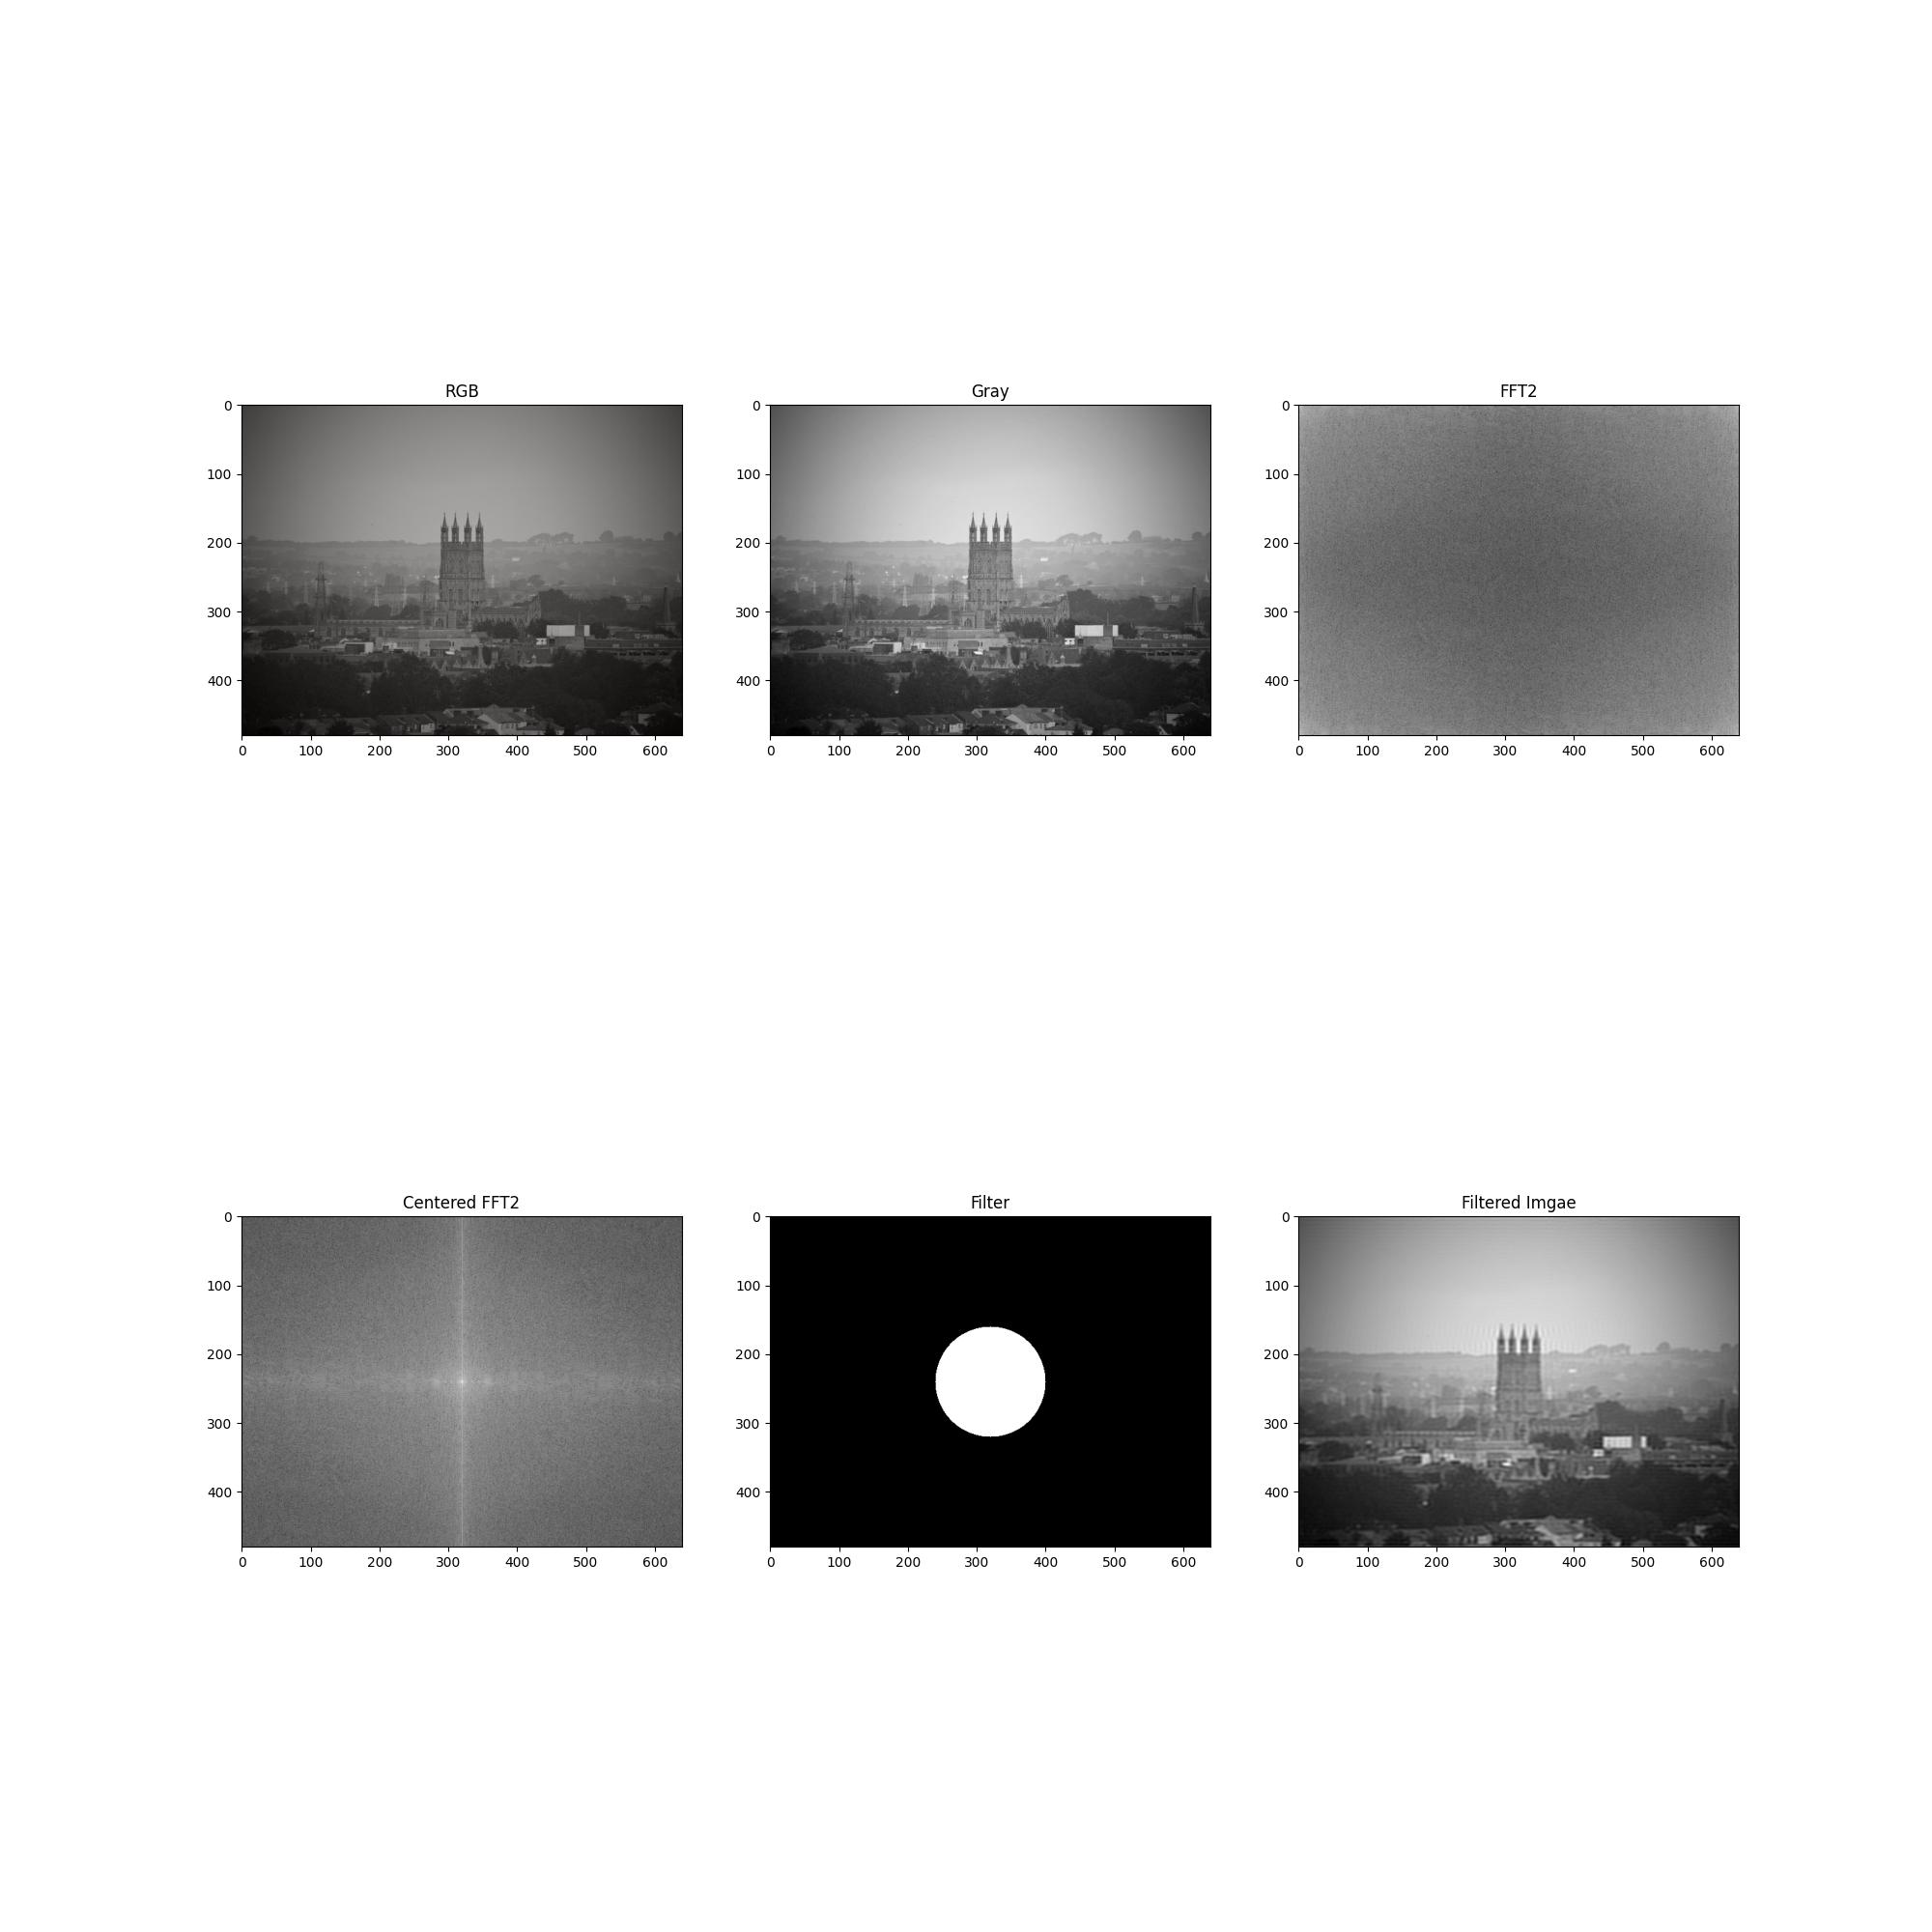
\includegraphics[width=0.7\textwidth]{Assignment-11/fig-v31.jpg}
            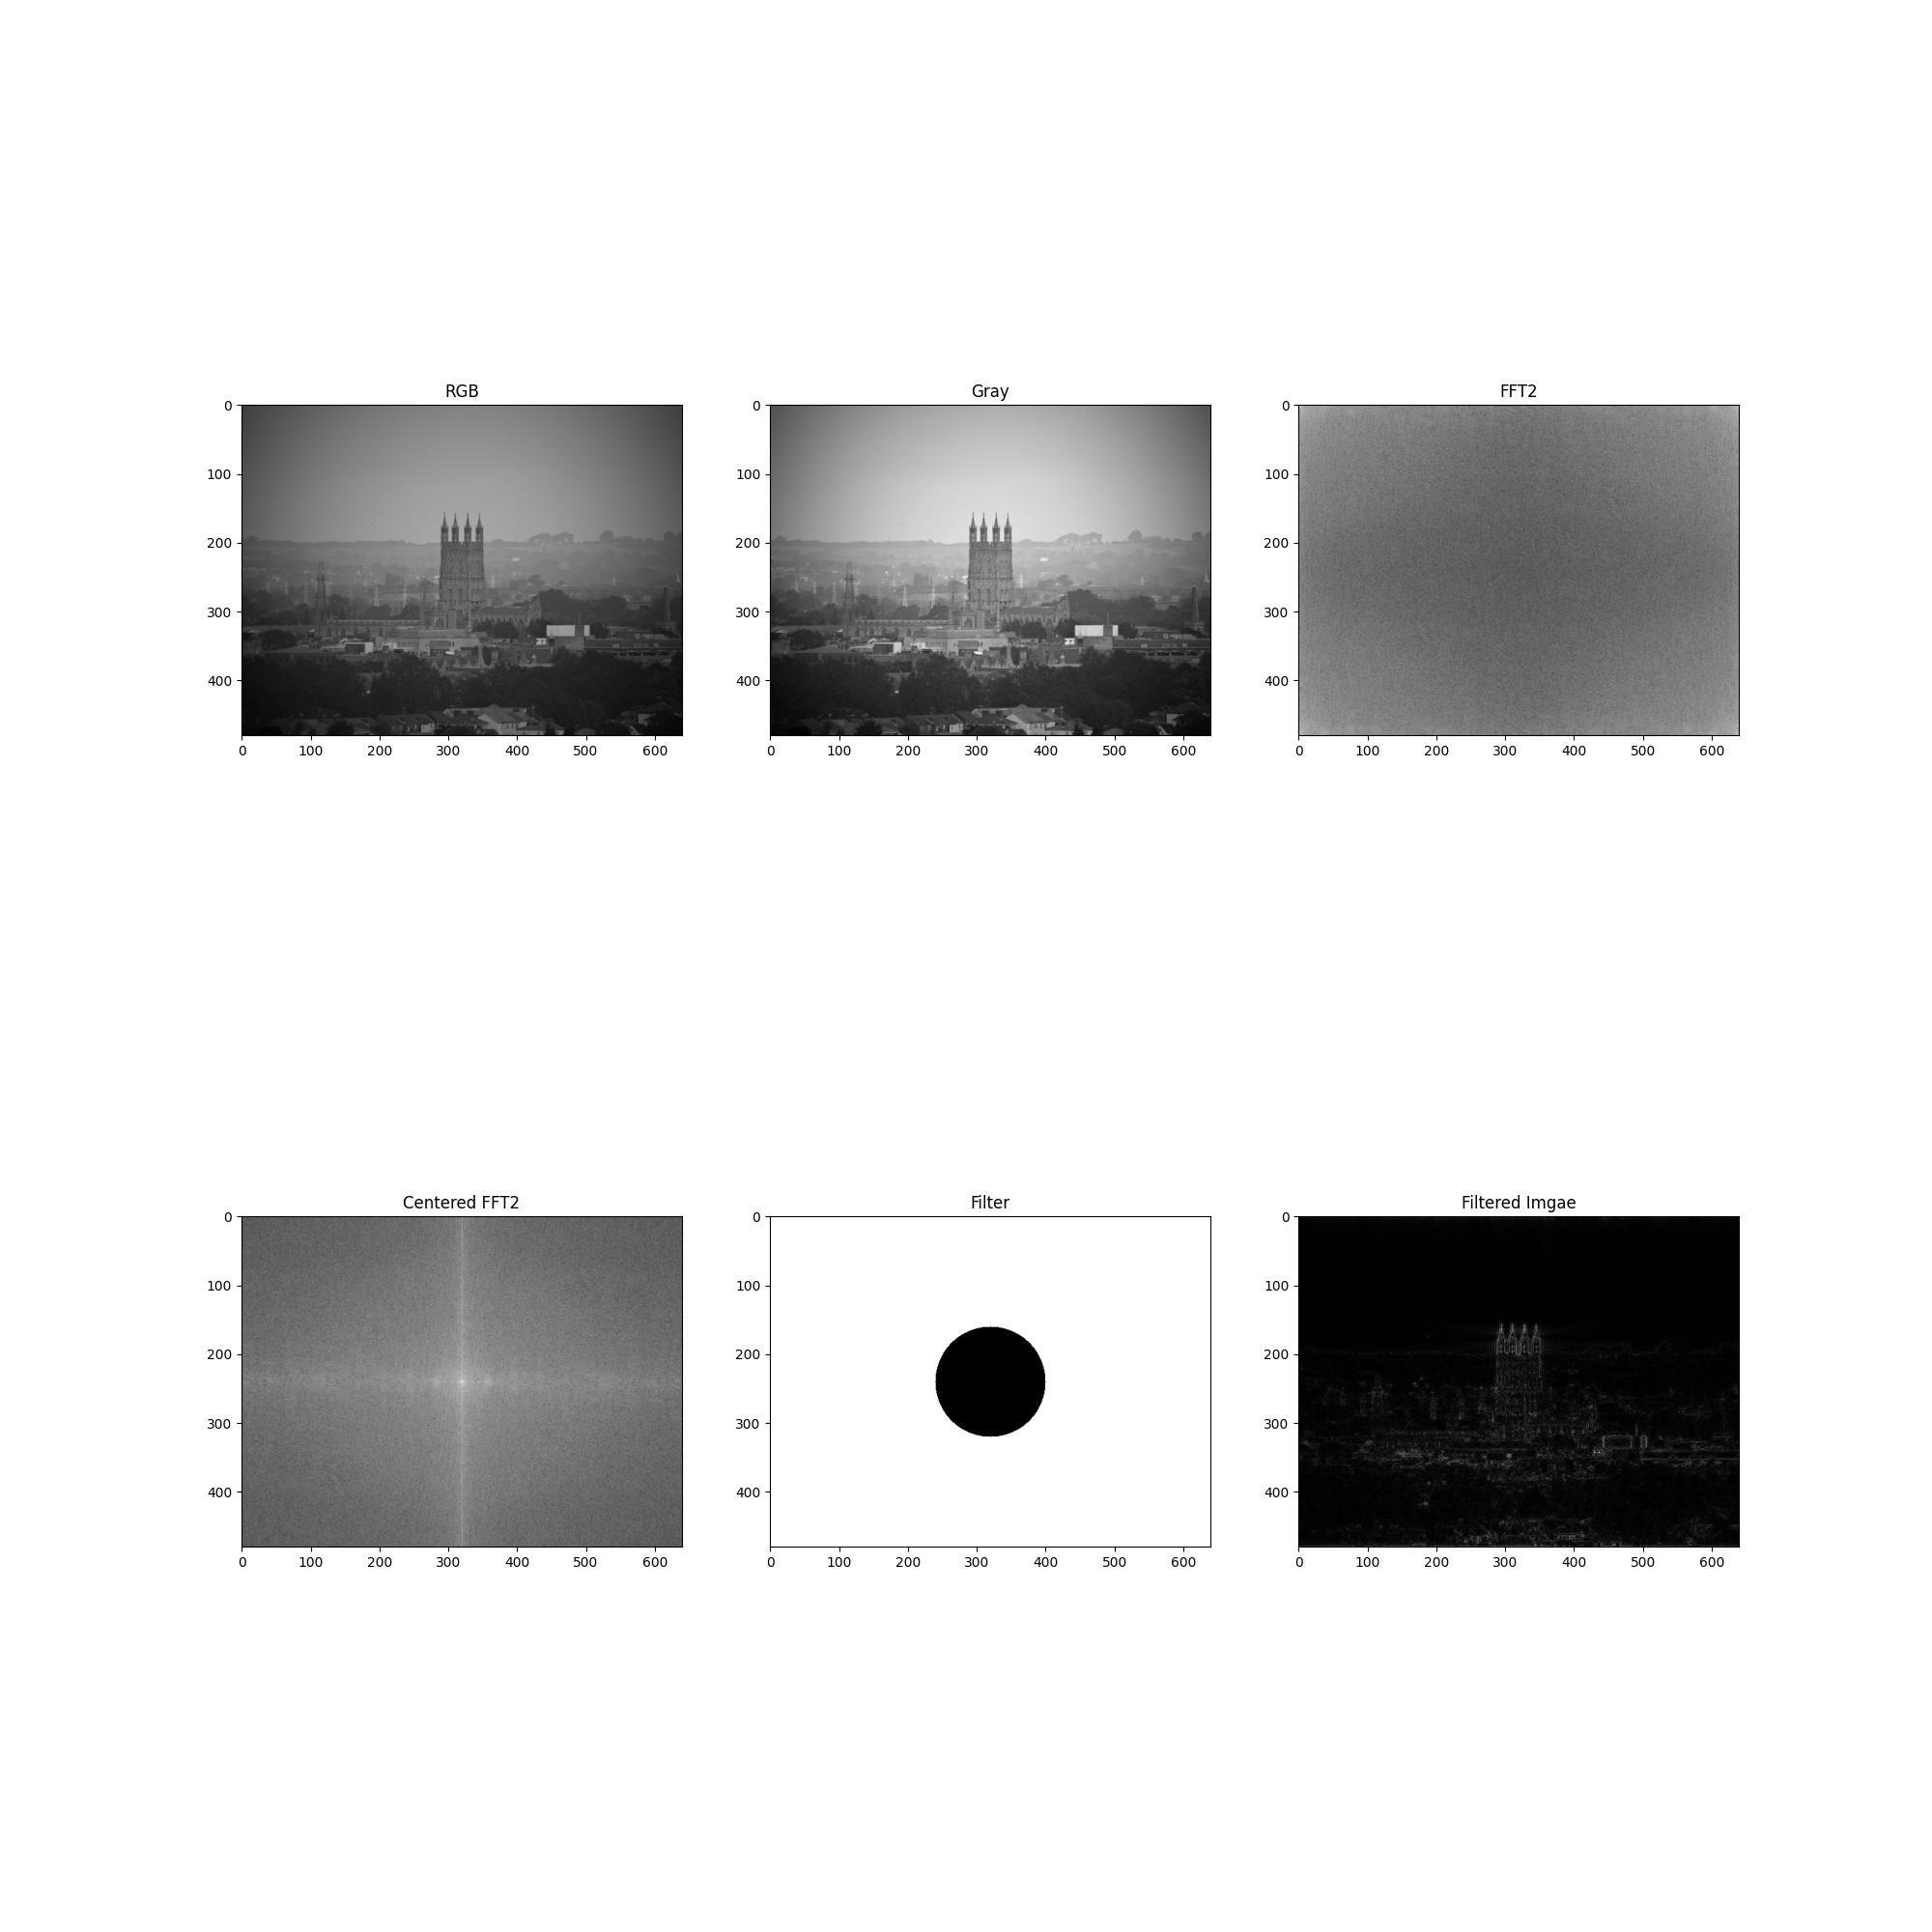
\includegraphics[width=0.7\textwidth]{Assignment-11/fig-v32.jpg}
            \caption{Outputs of filtering in frequency domain}
        \end{figure}
        \begin{figure}[htp]
            \centering
            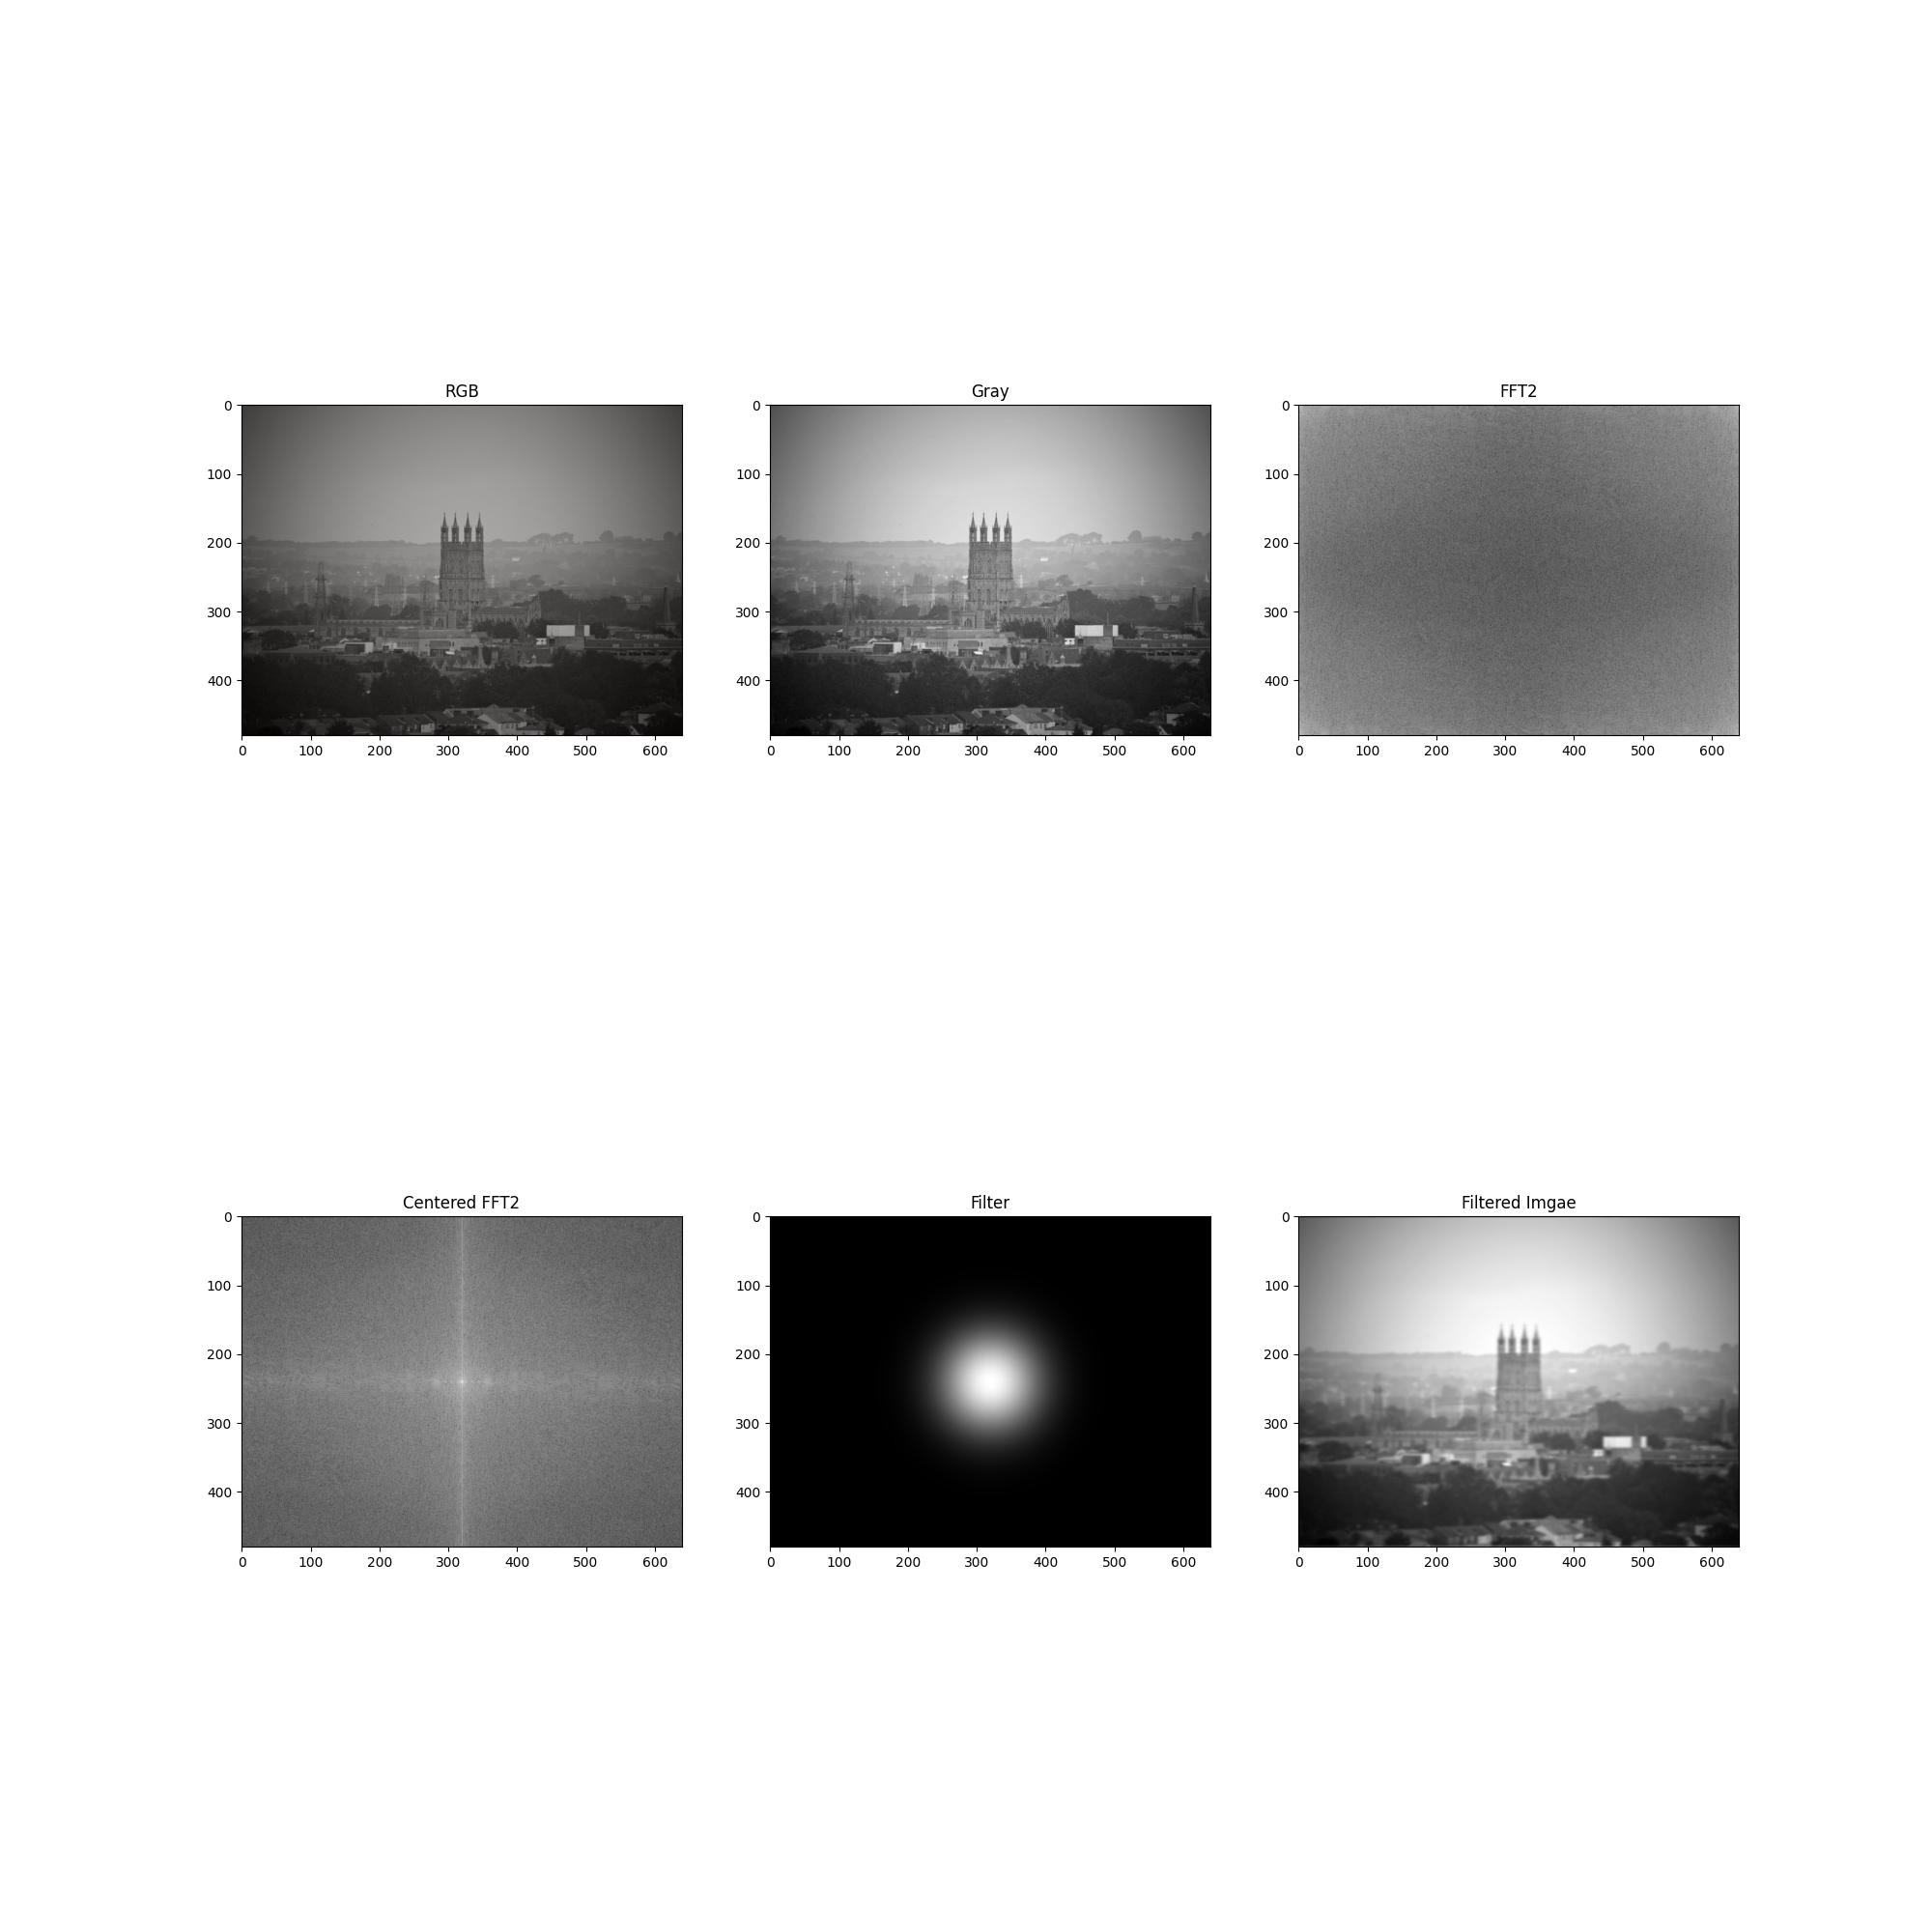
\includegraphics[width=0.7\textwidth]{Assignment-11/fig-v33.jpg}
            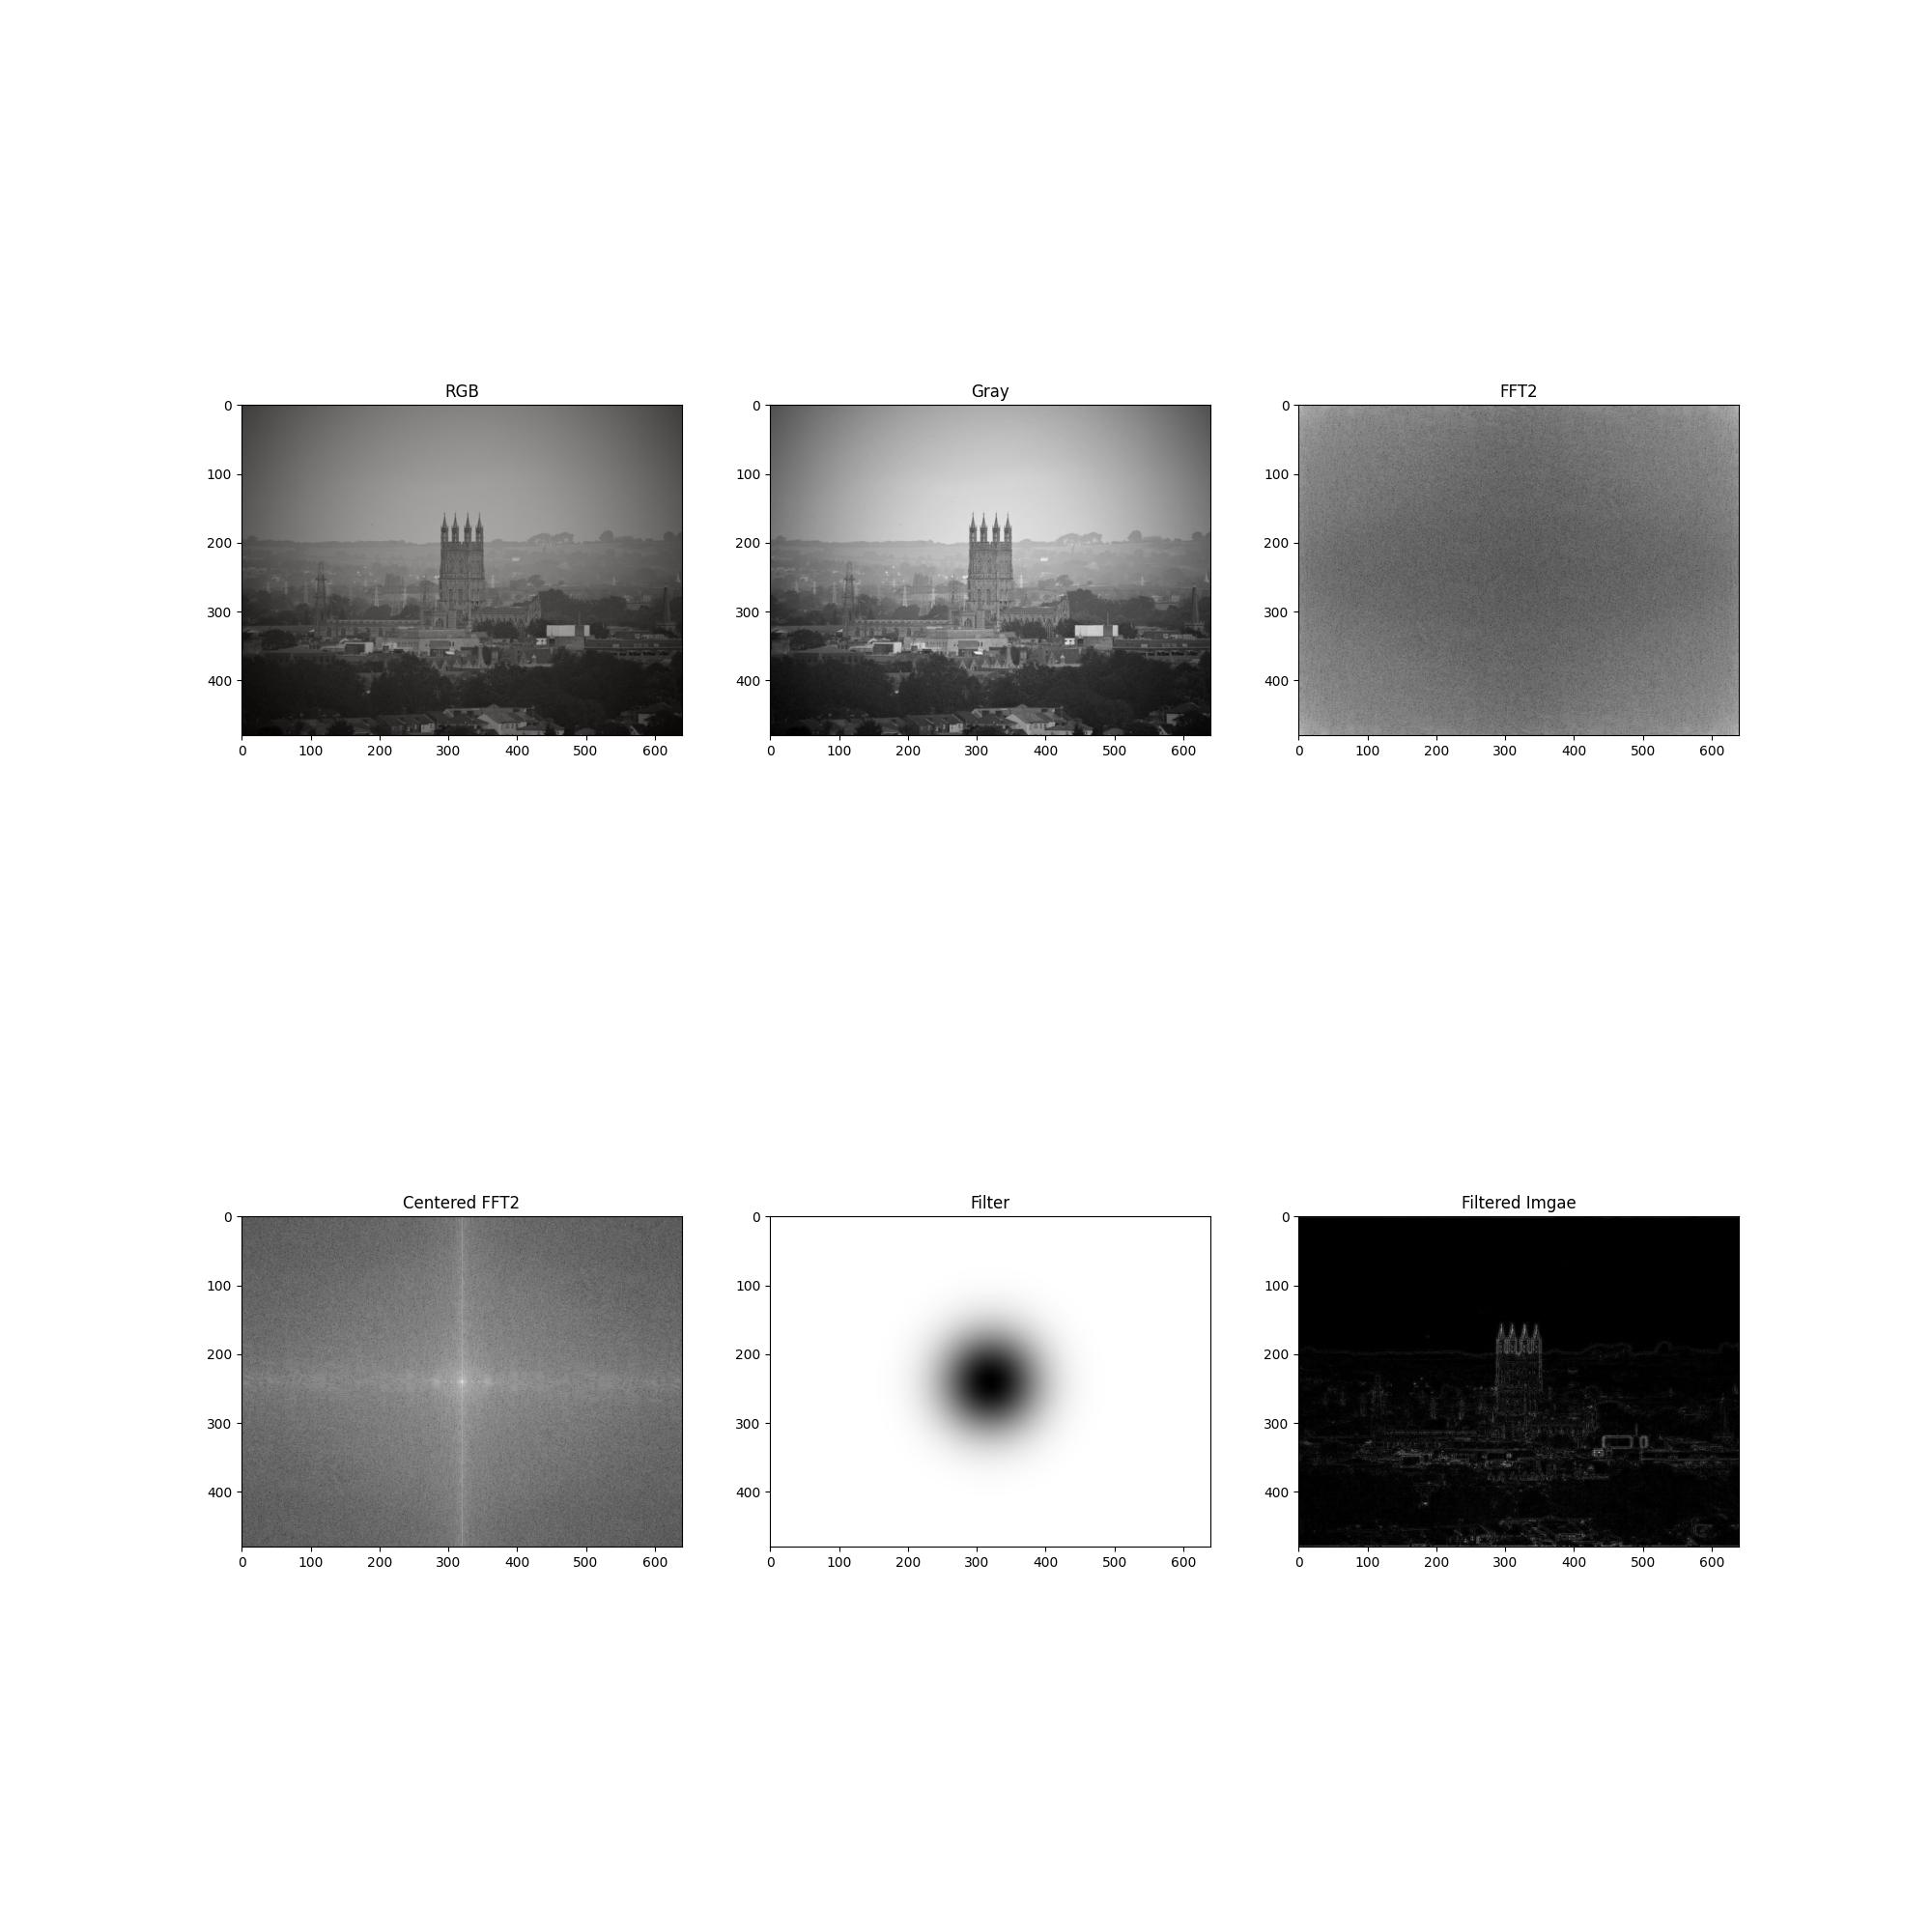
\includegraphics[width=0.7\textwidth]{Assignment-11/fig-v34.jpg}
            \caption{Outputs of filtering in frequency domain}
        \end{figure}
        \begin{figure}[htp]
            \centering
            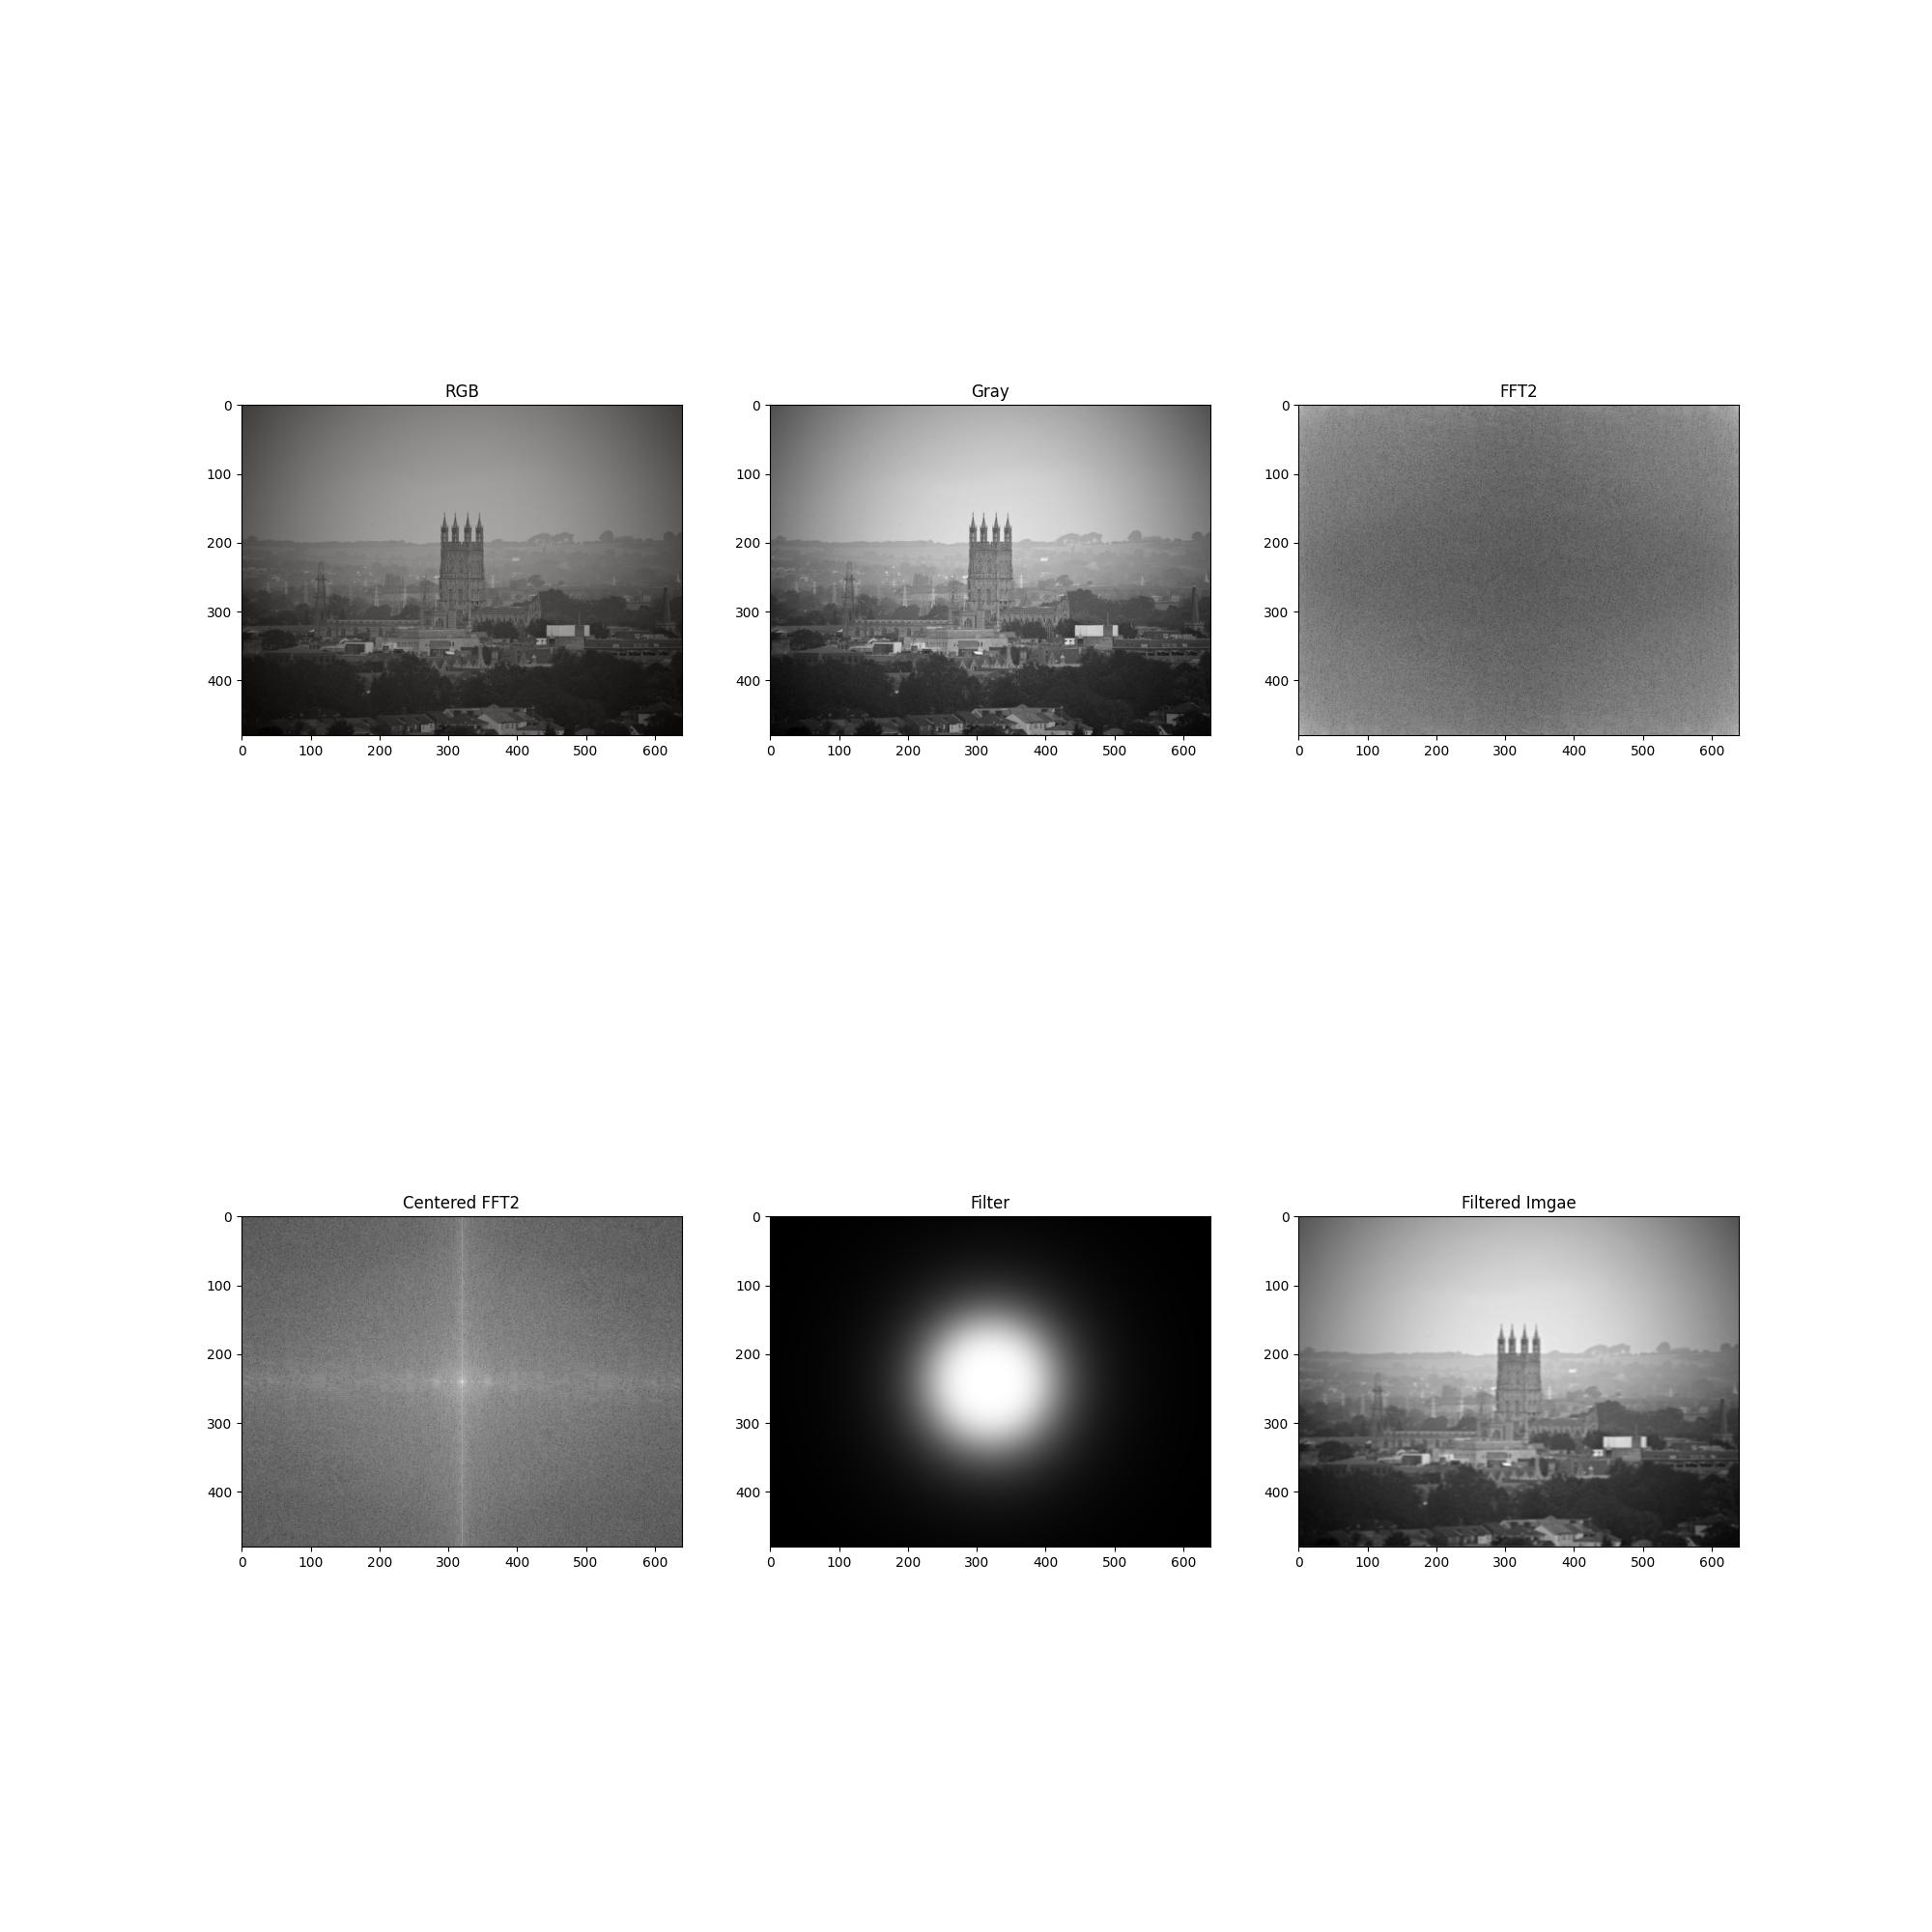
\includegraphics[width=0.7\textwidth]{Assignment-11/fig-v35.jpg}
            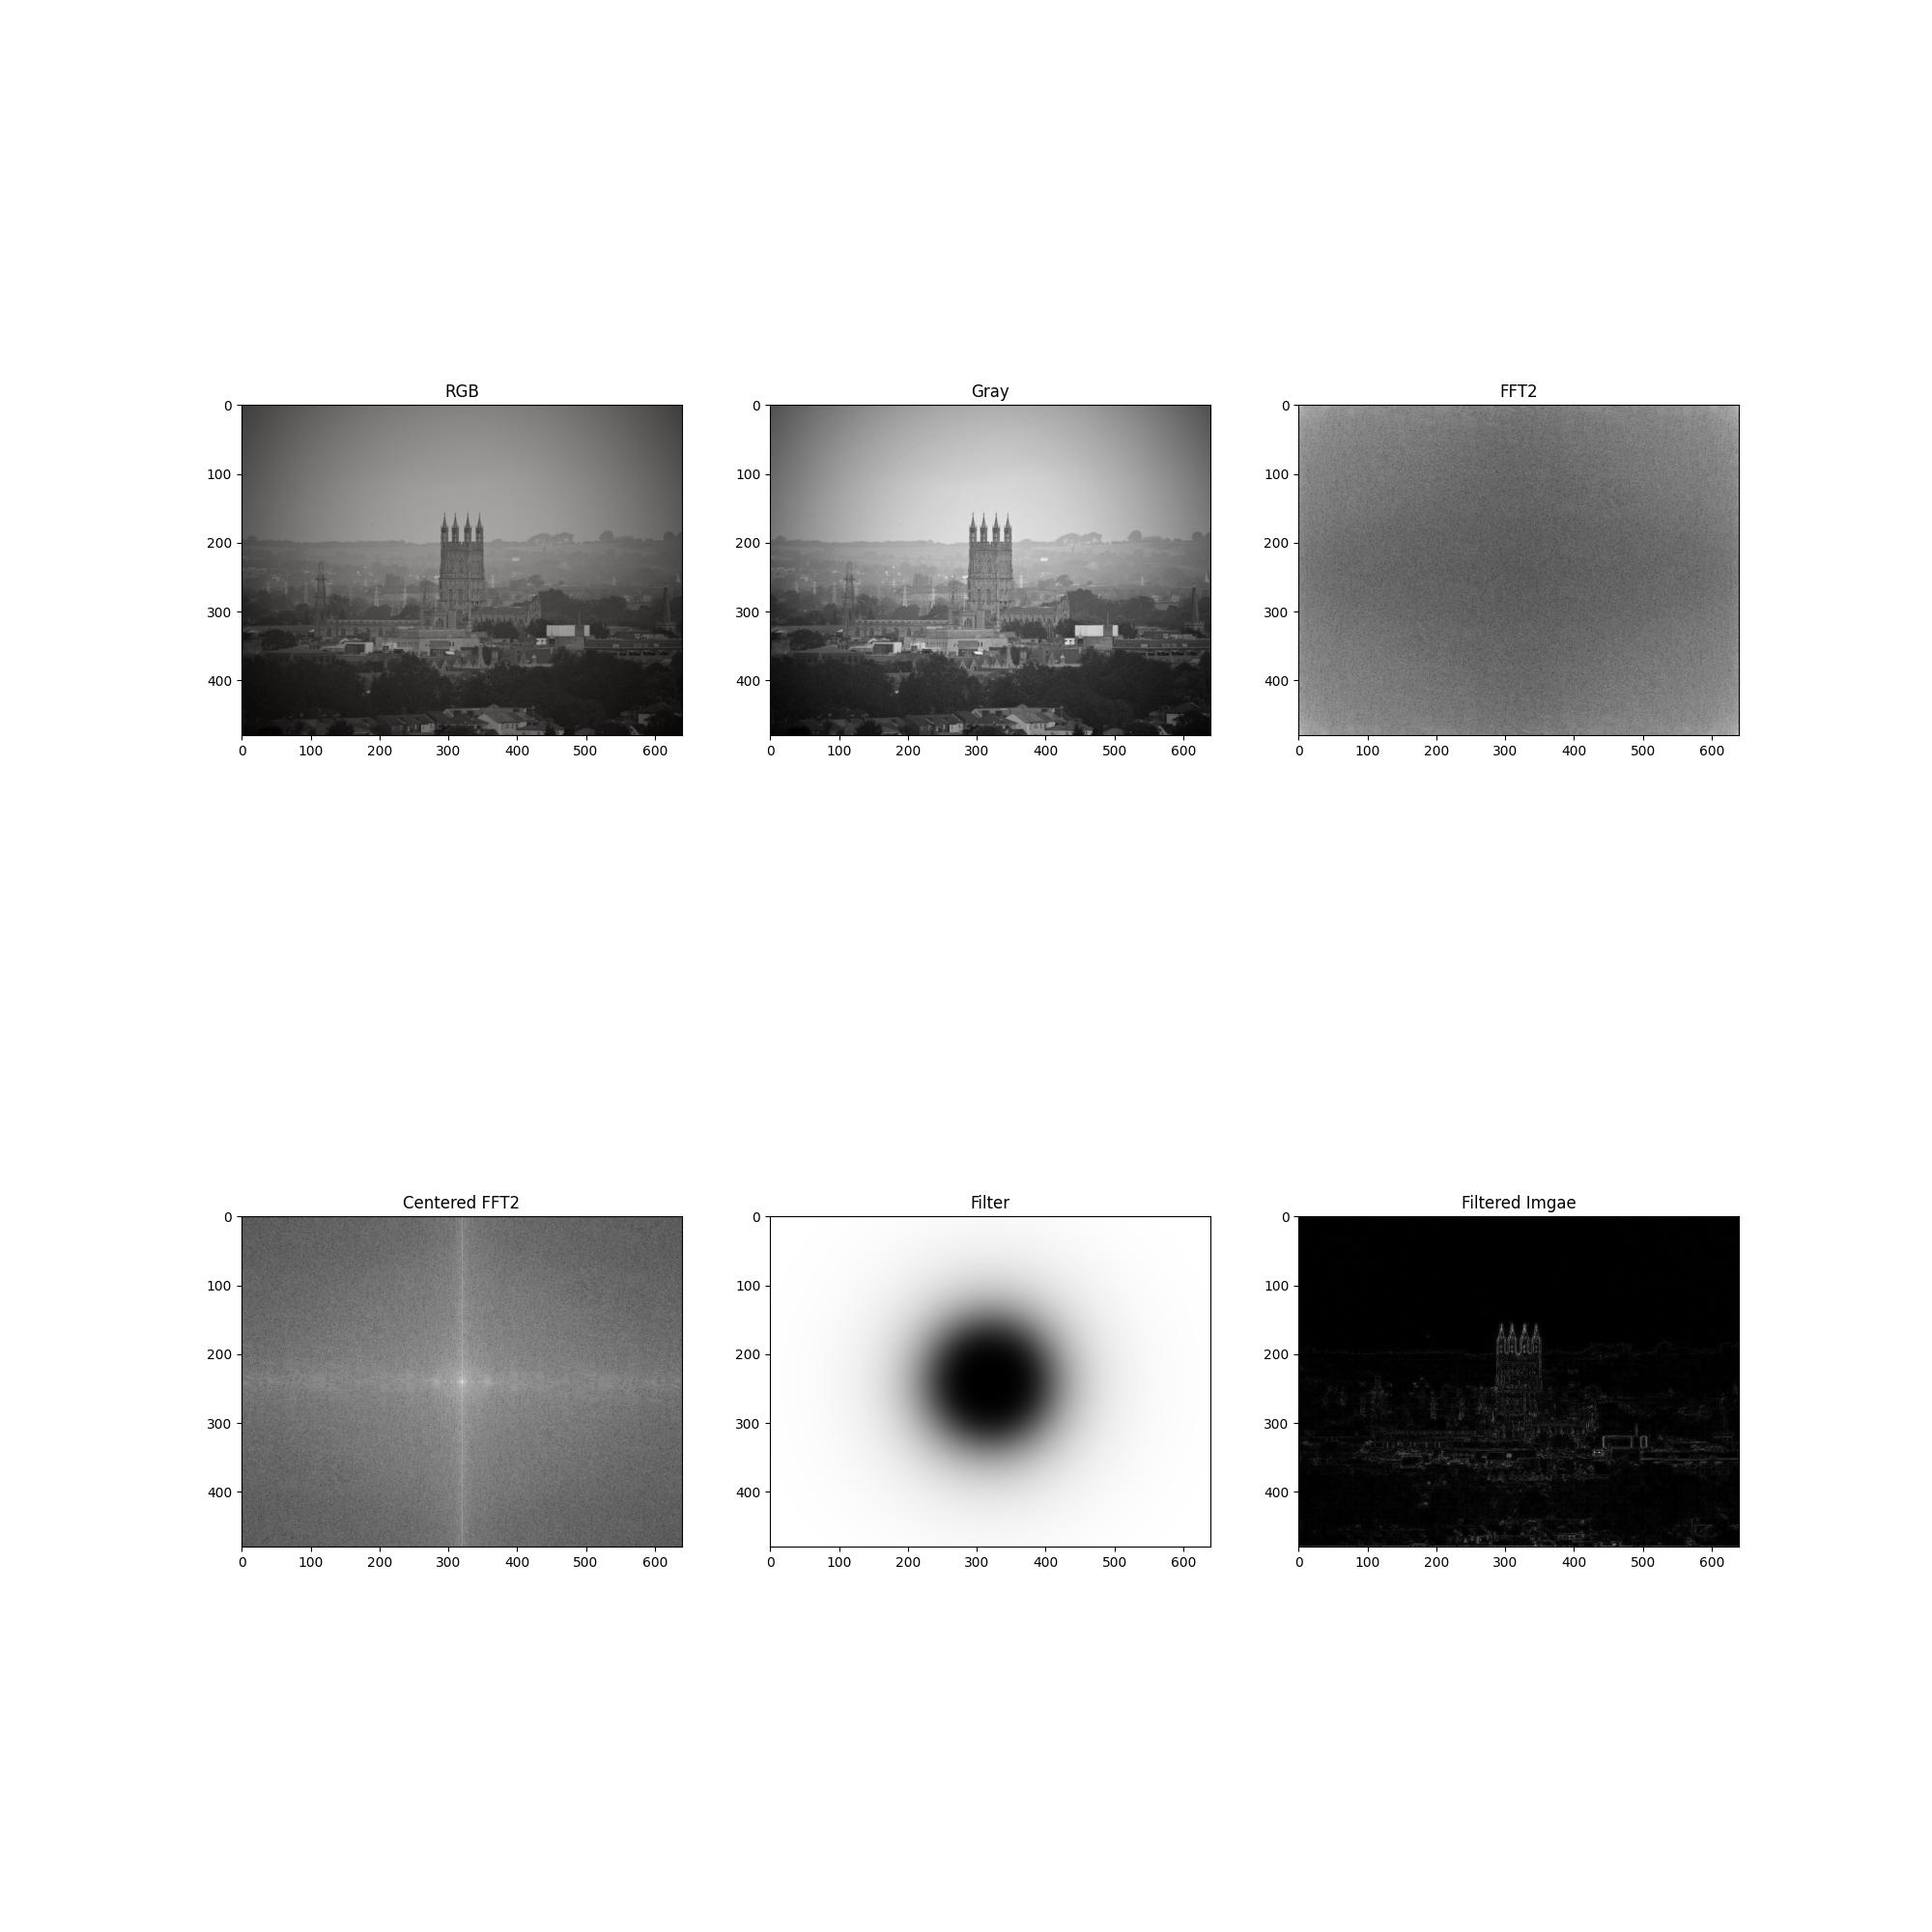
\includegraphics[width=0.7\textwidth]{Assignment-11/fig-v36.jpg}
            \caption{Outputs of filtering in frequency domain}
        \end{figure}
    }
}
% \pagebreak
\clearpage

%-----------------------Assignment-12-------------------------%
{
    \section{Assignment-12}
    \subsection{Introduction}
    \textbf {Problem: }
    Write a report on what different convolution layers of a CNN based image classifier see. You may use the attached code. You need to install Tensorflow in your computer. You can run it in Google Colab for GPU support if you do not have GPU or enough memory.\\
    \\
    \textbf{Solution: }
    Here we have provide a report on what happens on different convolution layers of a CNN based image classifier. As the CNN model uses different layers, we can see different things happens to the images in different layers. The result and code of it given as follows.\\
    
    \subsection{Required Software}
    Here we have to install tensorflow which should be installed in a virtual environment. So at fist we have to create a virtual environment then install tensorflow. Again in the virtual environment, we have to install matplotlib, opencv and tk for generating the output. For the first execution of the program, the tensorflow model has to be loaded, so it will take some time to download. After that the program will execute fast.\\
    
    \subsection{Procedure}
    \textbf{Step-1:}
    Install tensorflow, matplotlib, opencv libraries.\\
    \textbf{Step-2:}
    Run the following code.\\
    
    \subsection{Code}
    \lstset{style=mystyle}
    \begin{lstlisting}[language=Python, caption=Code for using pre trained model(VGG16)]
    from tensorflow.keras.applications.vgg16 import VGG16, preprocess_input
    import cv2
    import matplotlib.pyplot as plt
    import numpy as np
    from tensorflow.keras.models import Model
    
    DIR = '/media/mursalin/New Volume/Image-Processing/code_13/'
    # DIR = './'
    
    def main():
    	# Load a pre-trained model.
    	baseModel = VGG16()
    	baseModel.summary()
    		
    	# Prepare a new model having the desired layer as the output layer.
    	for i in range(10): 
    		layer_number = i +1# *** Change layer number to see different convolution layer's output.
    		print(layer_number)
    		inputs = baseModel.input
    		outputs = baseModel.layers[layer_number].output
    		model = Model(inputs, outputs)
    
    		# Prepare data.
    		img = prepare_data()
    
    		# Predict output of a specific layer.
    		outputs = model.predict(img)
    	
    		# Display what different channls see.
    		display_channels(outputs, layer_number)
    	
    def display_channels(chSet, layer_no):	
    	plt.figure(figsize = (20, 20))
    	plt.suptitle('Layer-' + str(layer_no))
    	for i in range(9):
    		plt.subplot(3, 3, i + 1)
    		plt.title('Channel-' + str(i))
    		plt.imshow(chSet[0, :, :, i], cmap = 'gray')
    		plt.axis('off')
    	
    	plt.savefig(DIR+'fig-'+str(layer_no)+'.jpg')
    	plt.show()
    	plt.close()
    	
    def prepare_data():
    	# Load an image
    	imgPath = DIR + 'rose.jpg'	#'Elephant.jpg' #'Baby.jpeg' #'Rose.jpeg' #'Boat.jpeg' #	
    	bgrImg = cv2.imread(imgPath)
    	print(bgrImg.shape)
    	
    	# Convert the image from BGR into RGB format
    	rgbImg = cv2.cvtColor(bgrImg, cv2.COLOR_BGR2RGB)
    	
    	# Reshape the image so that it can fit into the model.
    	#display_img(rgbImg)
    	rgbImg = cv2.resize(rgbImg, (224, 224))
    	display_img(rgbImg)
    	
    	# Expand dimension since the model accepts 4D data.
    	print(rgbImg.shape)
    	rgbImg = np.expand_dims(rgbImg, axis = 0)
    	print(rgbImg.shape)
    	
    	# Preprocess image
    	rgbImg = preprocess_input(rgbImg)
    	
    	return rgbImg
    	
    def display_img(img):
    	plt.imshow(img)
    	plt.show()
    	plt.close()
    
    if __name__ == '__main__':
    	main()

    \end{lstlisting}
    \\
    \subsection{Result & Discussion}{
        As we are using the VGG16 model as CNN model, there are 16 different layers are produced here. As different convolution layer are present there, so if we give input of an image, we will get different kinds of output for each kind of layers. For this experiment, we have taken output of 9 picture for each layer and found out the difference. The output picture of 10 different layers is given below. From the 1st layer, we can see that the output picture can easily be recognised. Here the edges of the object can easily be understood and here, sobel filter is perhaps used. From layer-2's output, the picture continues to become blur and at the end of layer 10, the picture can no more be understood. After the finished layer output, the picture can no more be recognised.
        
        \begin{figure}[htp]
            \begin{overprint}
                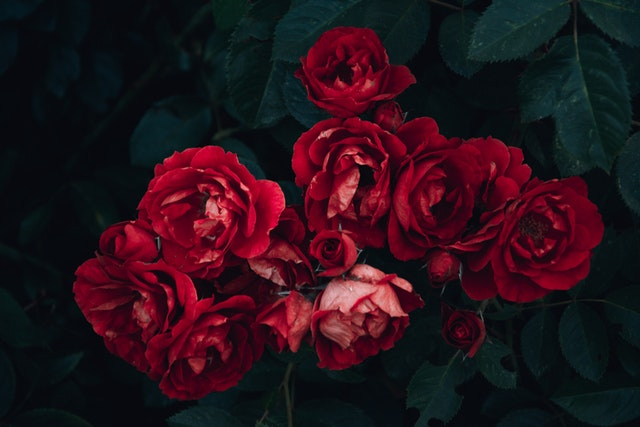
\includegraphics[width=0.33\textwidth]{Assignment-12/rose.jpg}
                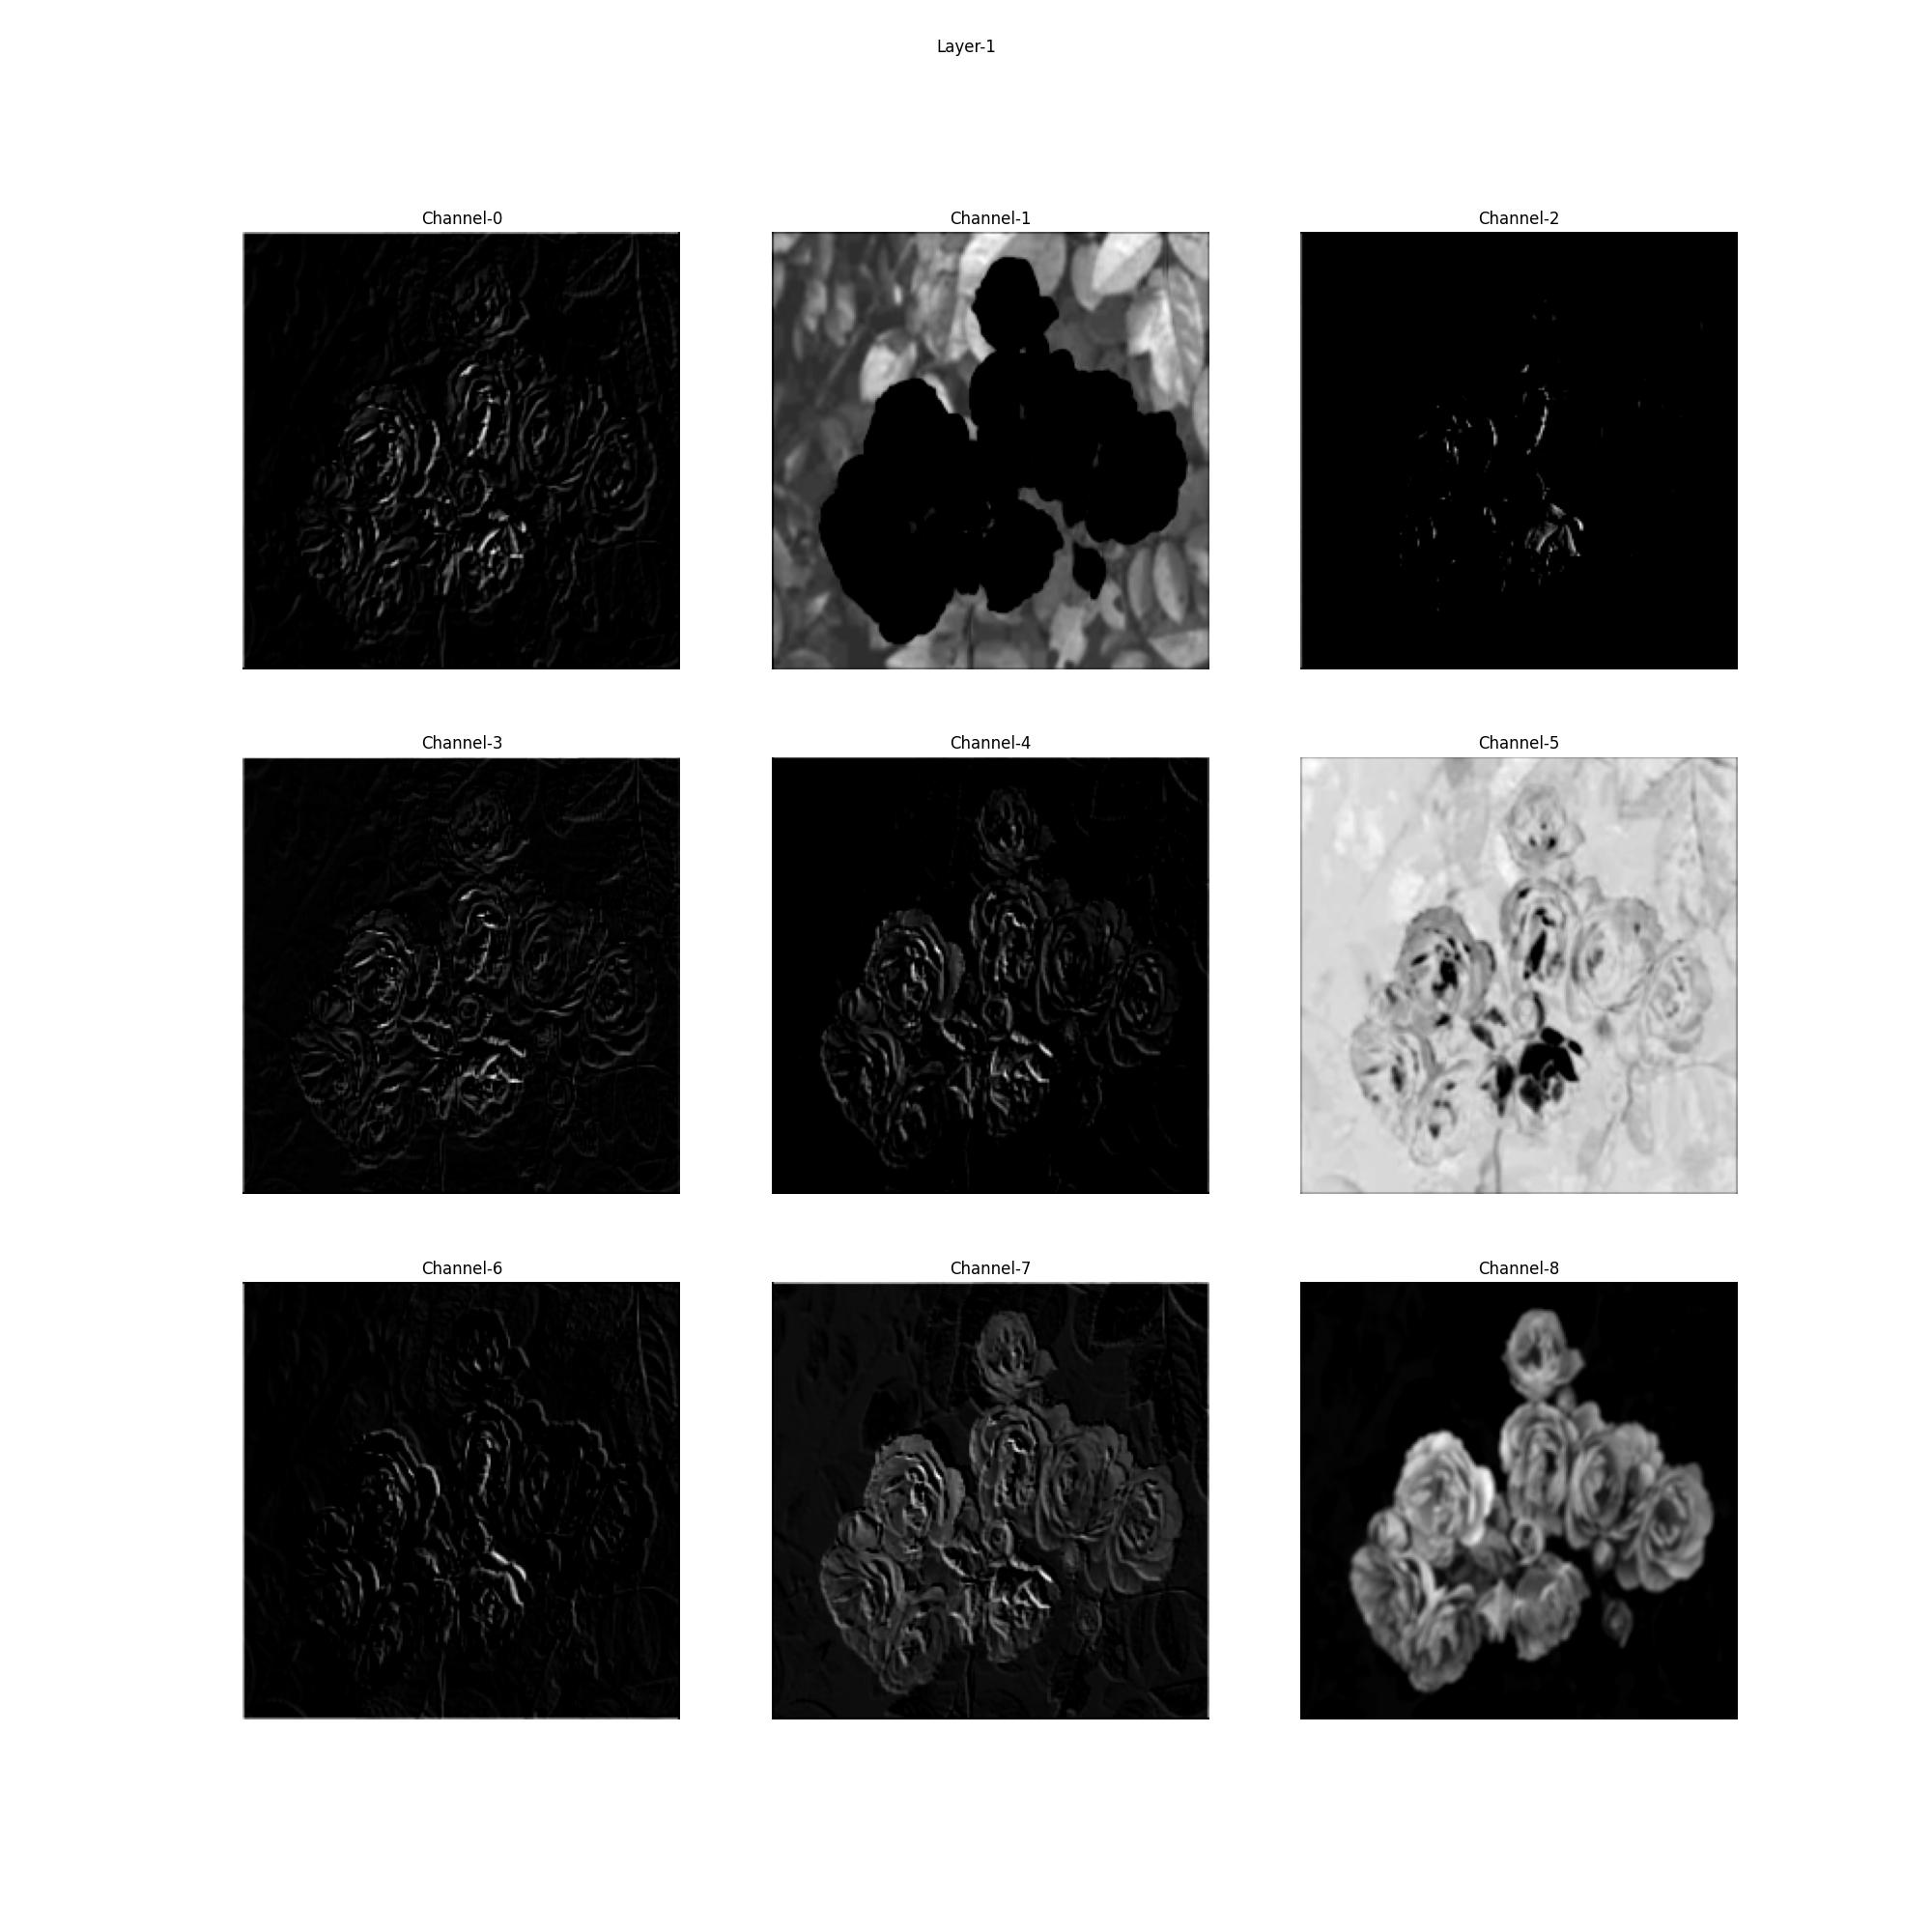
\includegraphics[width=0.33\textwidth]{Assignment-12/fig-1.jpg}
                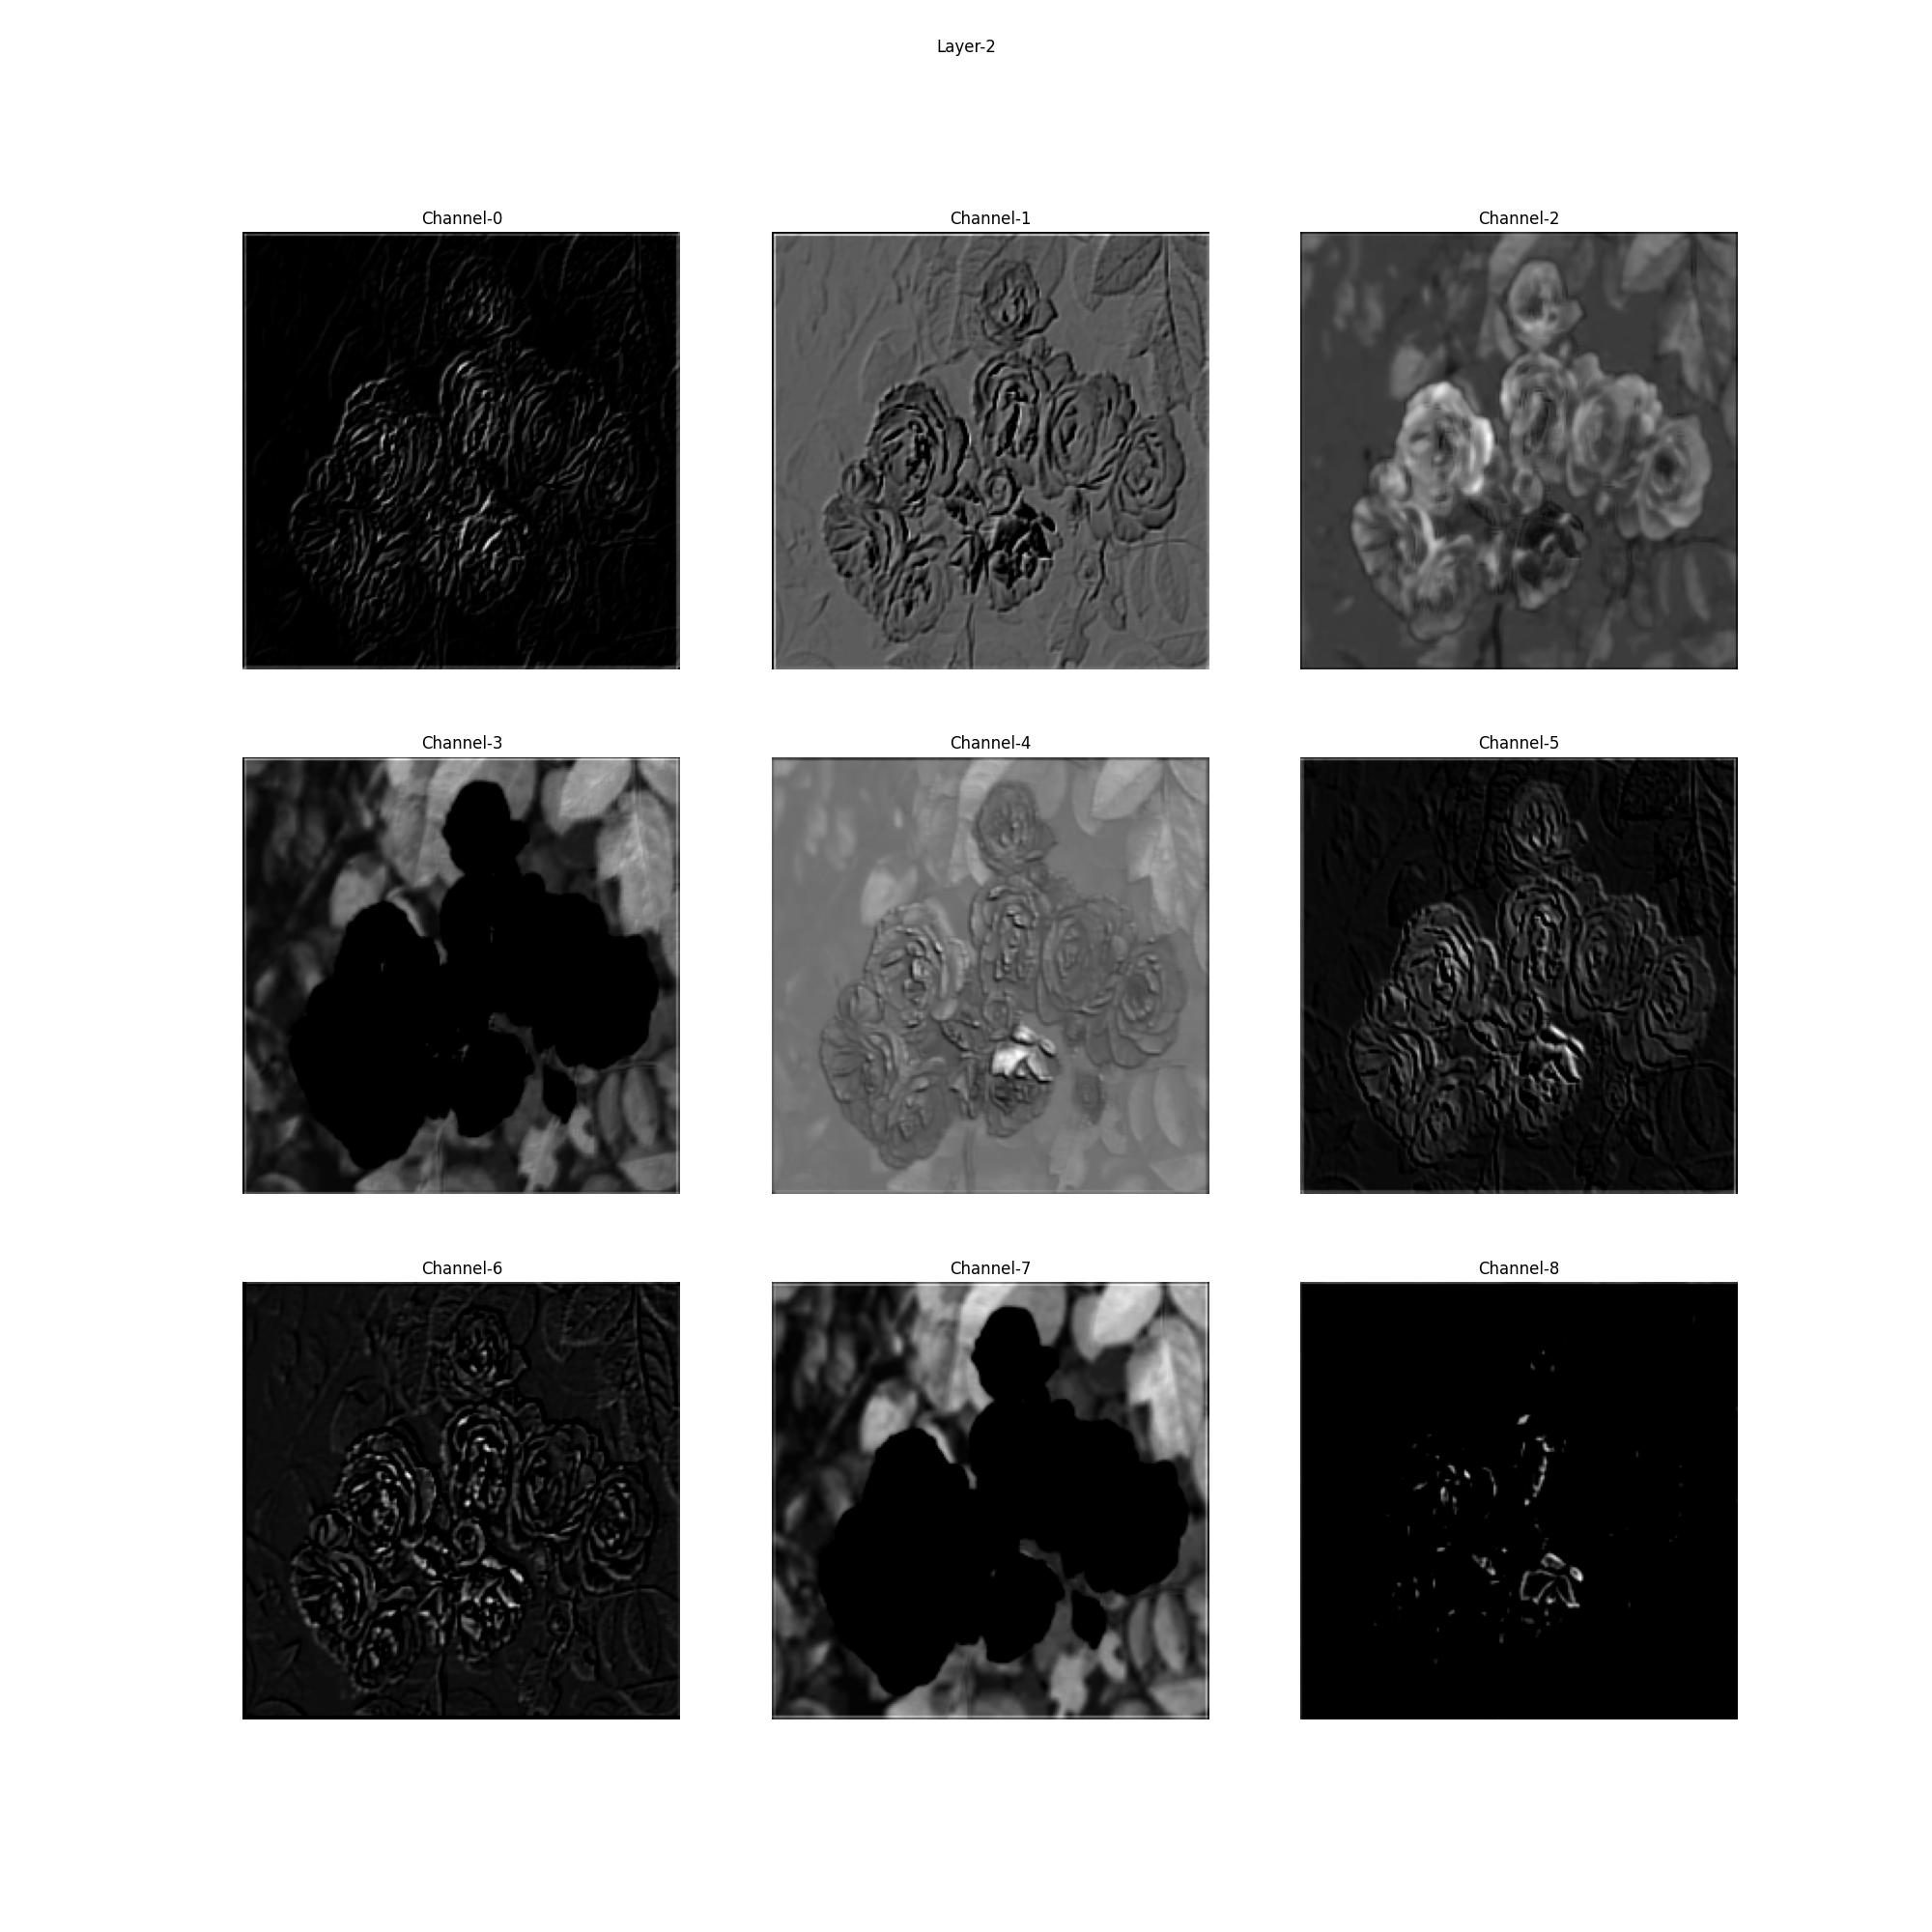
\includegraphics[width=0.33\textwidth]{Assignment-12/fig-2.jpg}
            \end{overprint}
            \begin{overprint}
                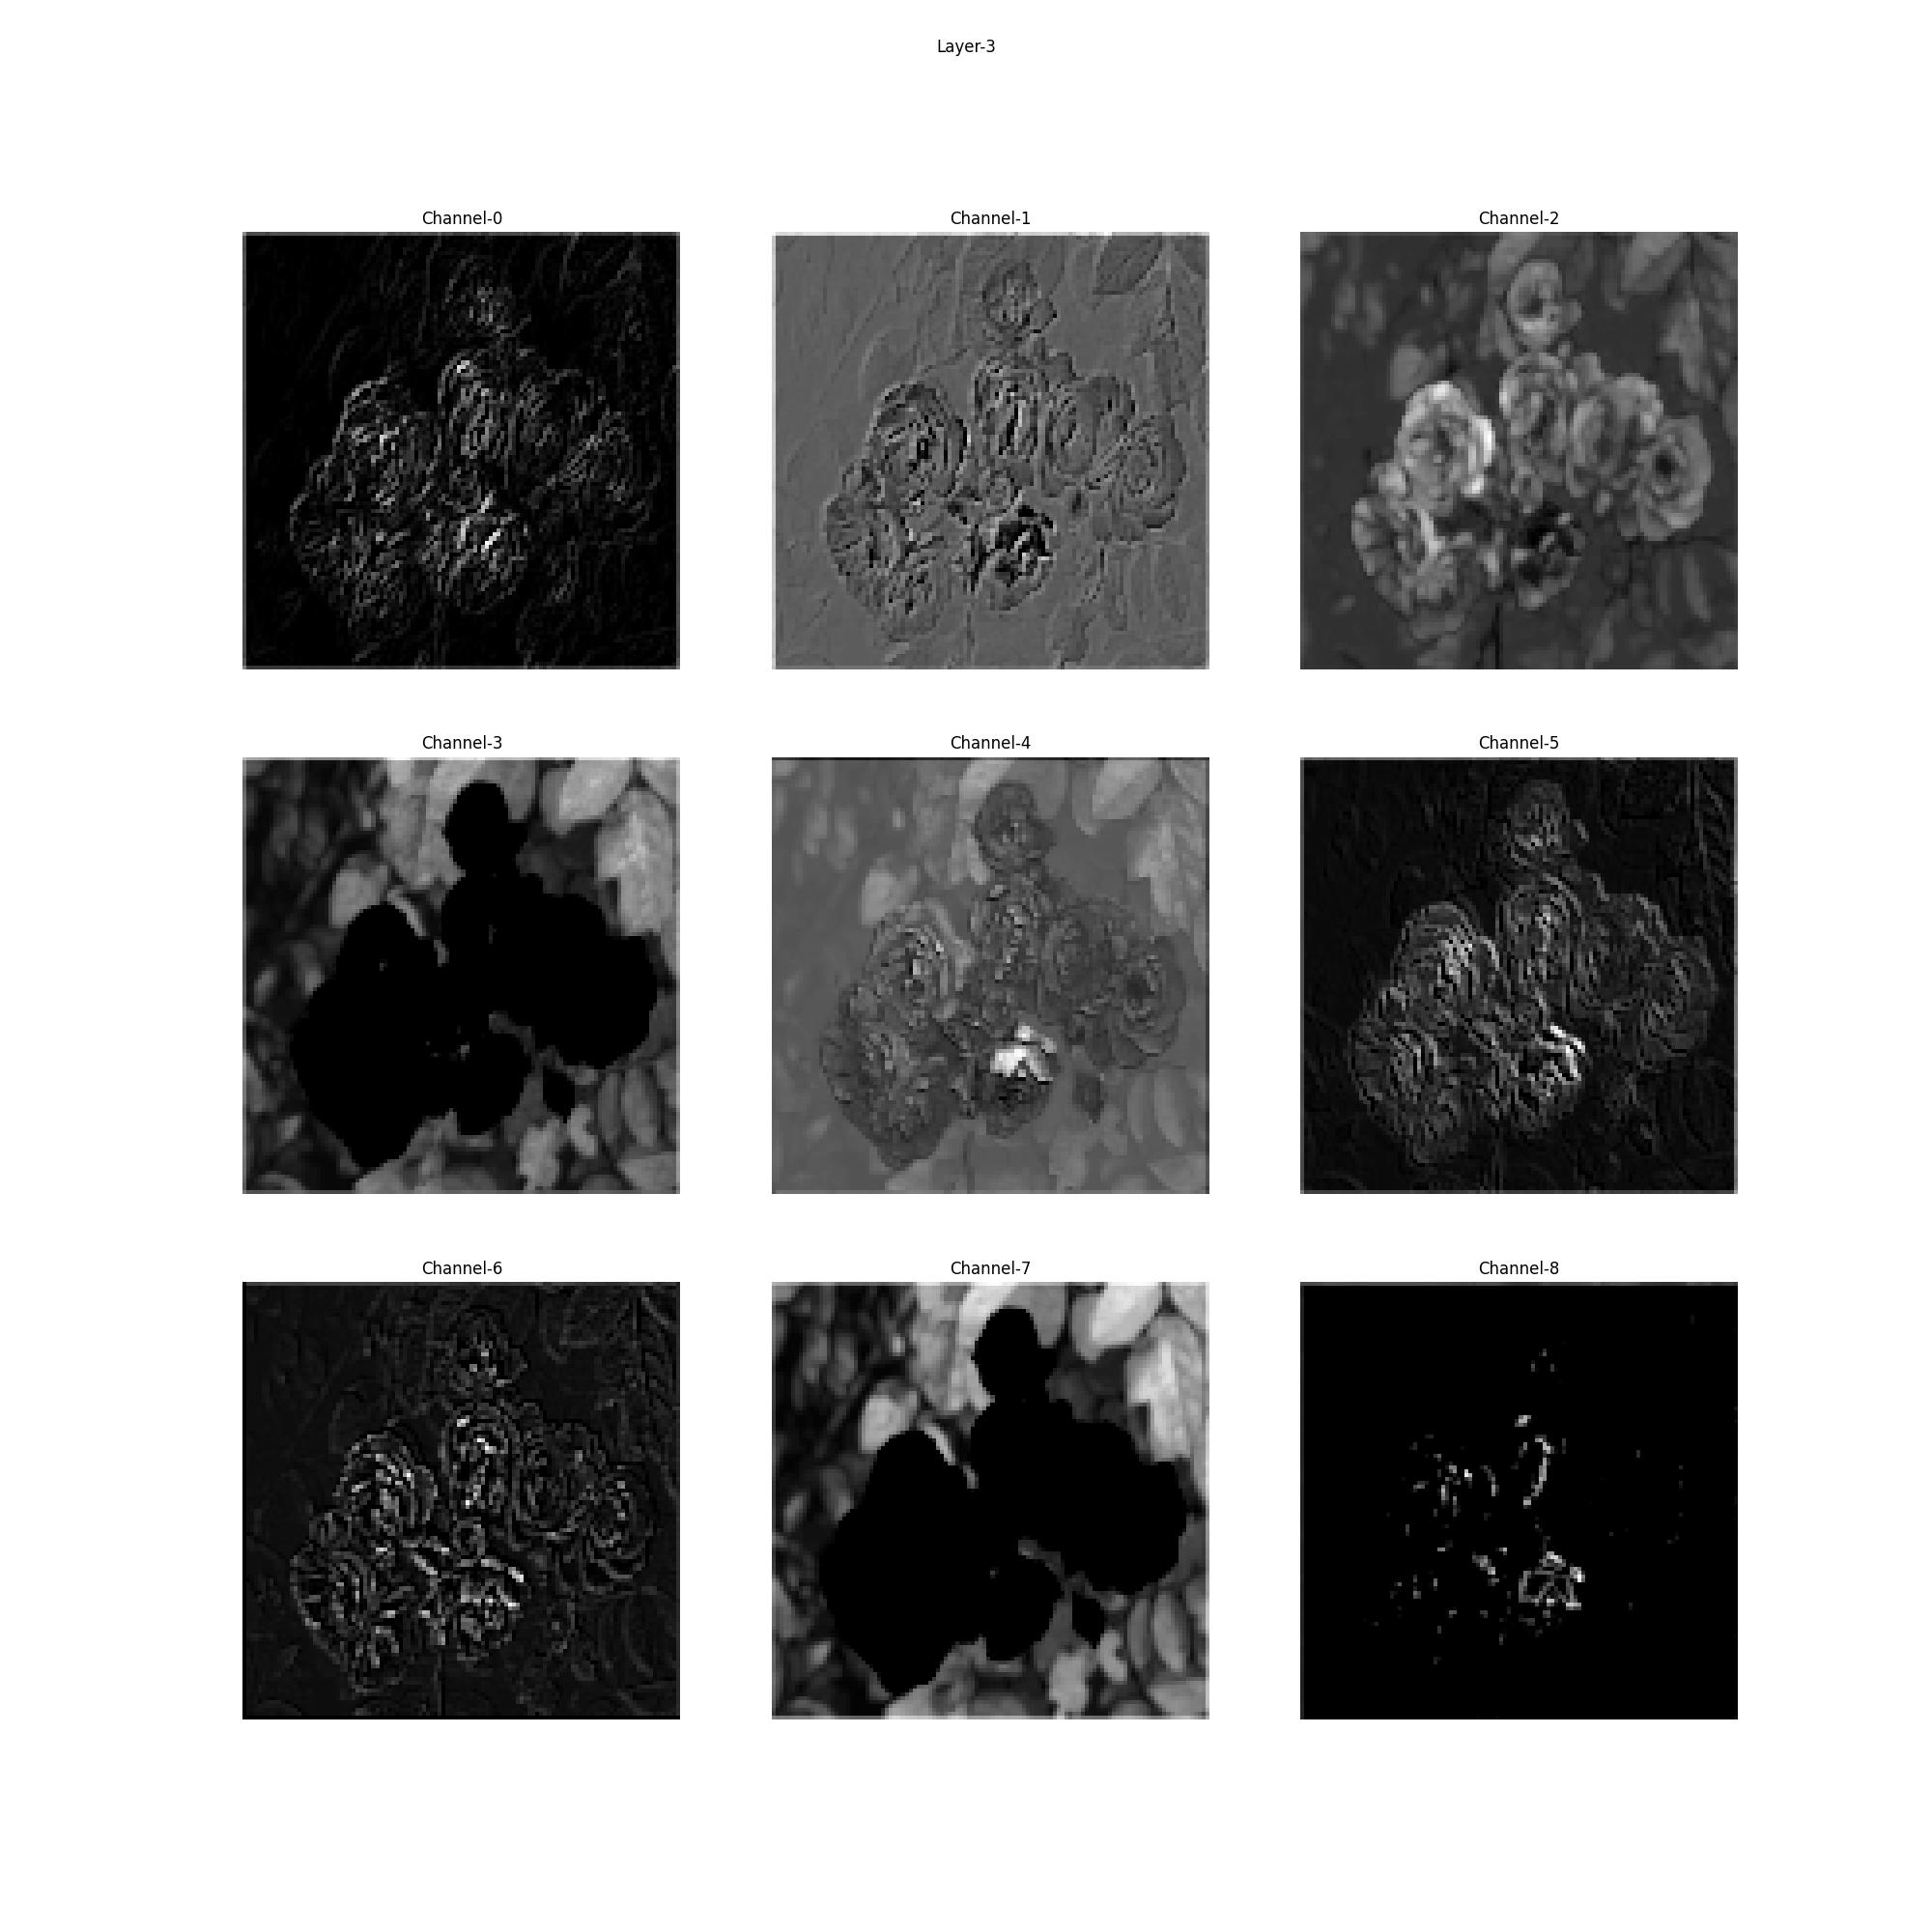
\includegraphics[width=0.33\textwidth]{Assignment-12/fig-3.jpg}
                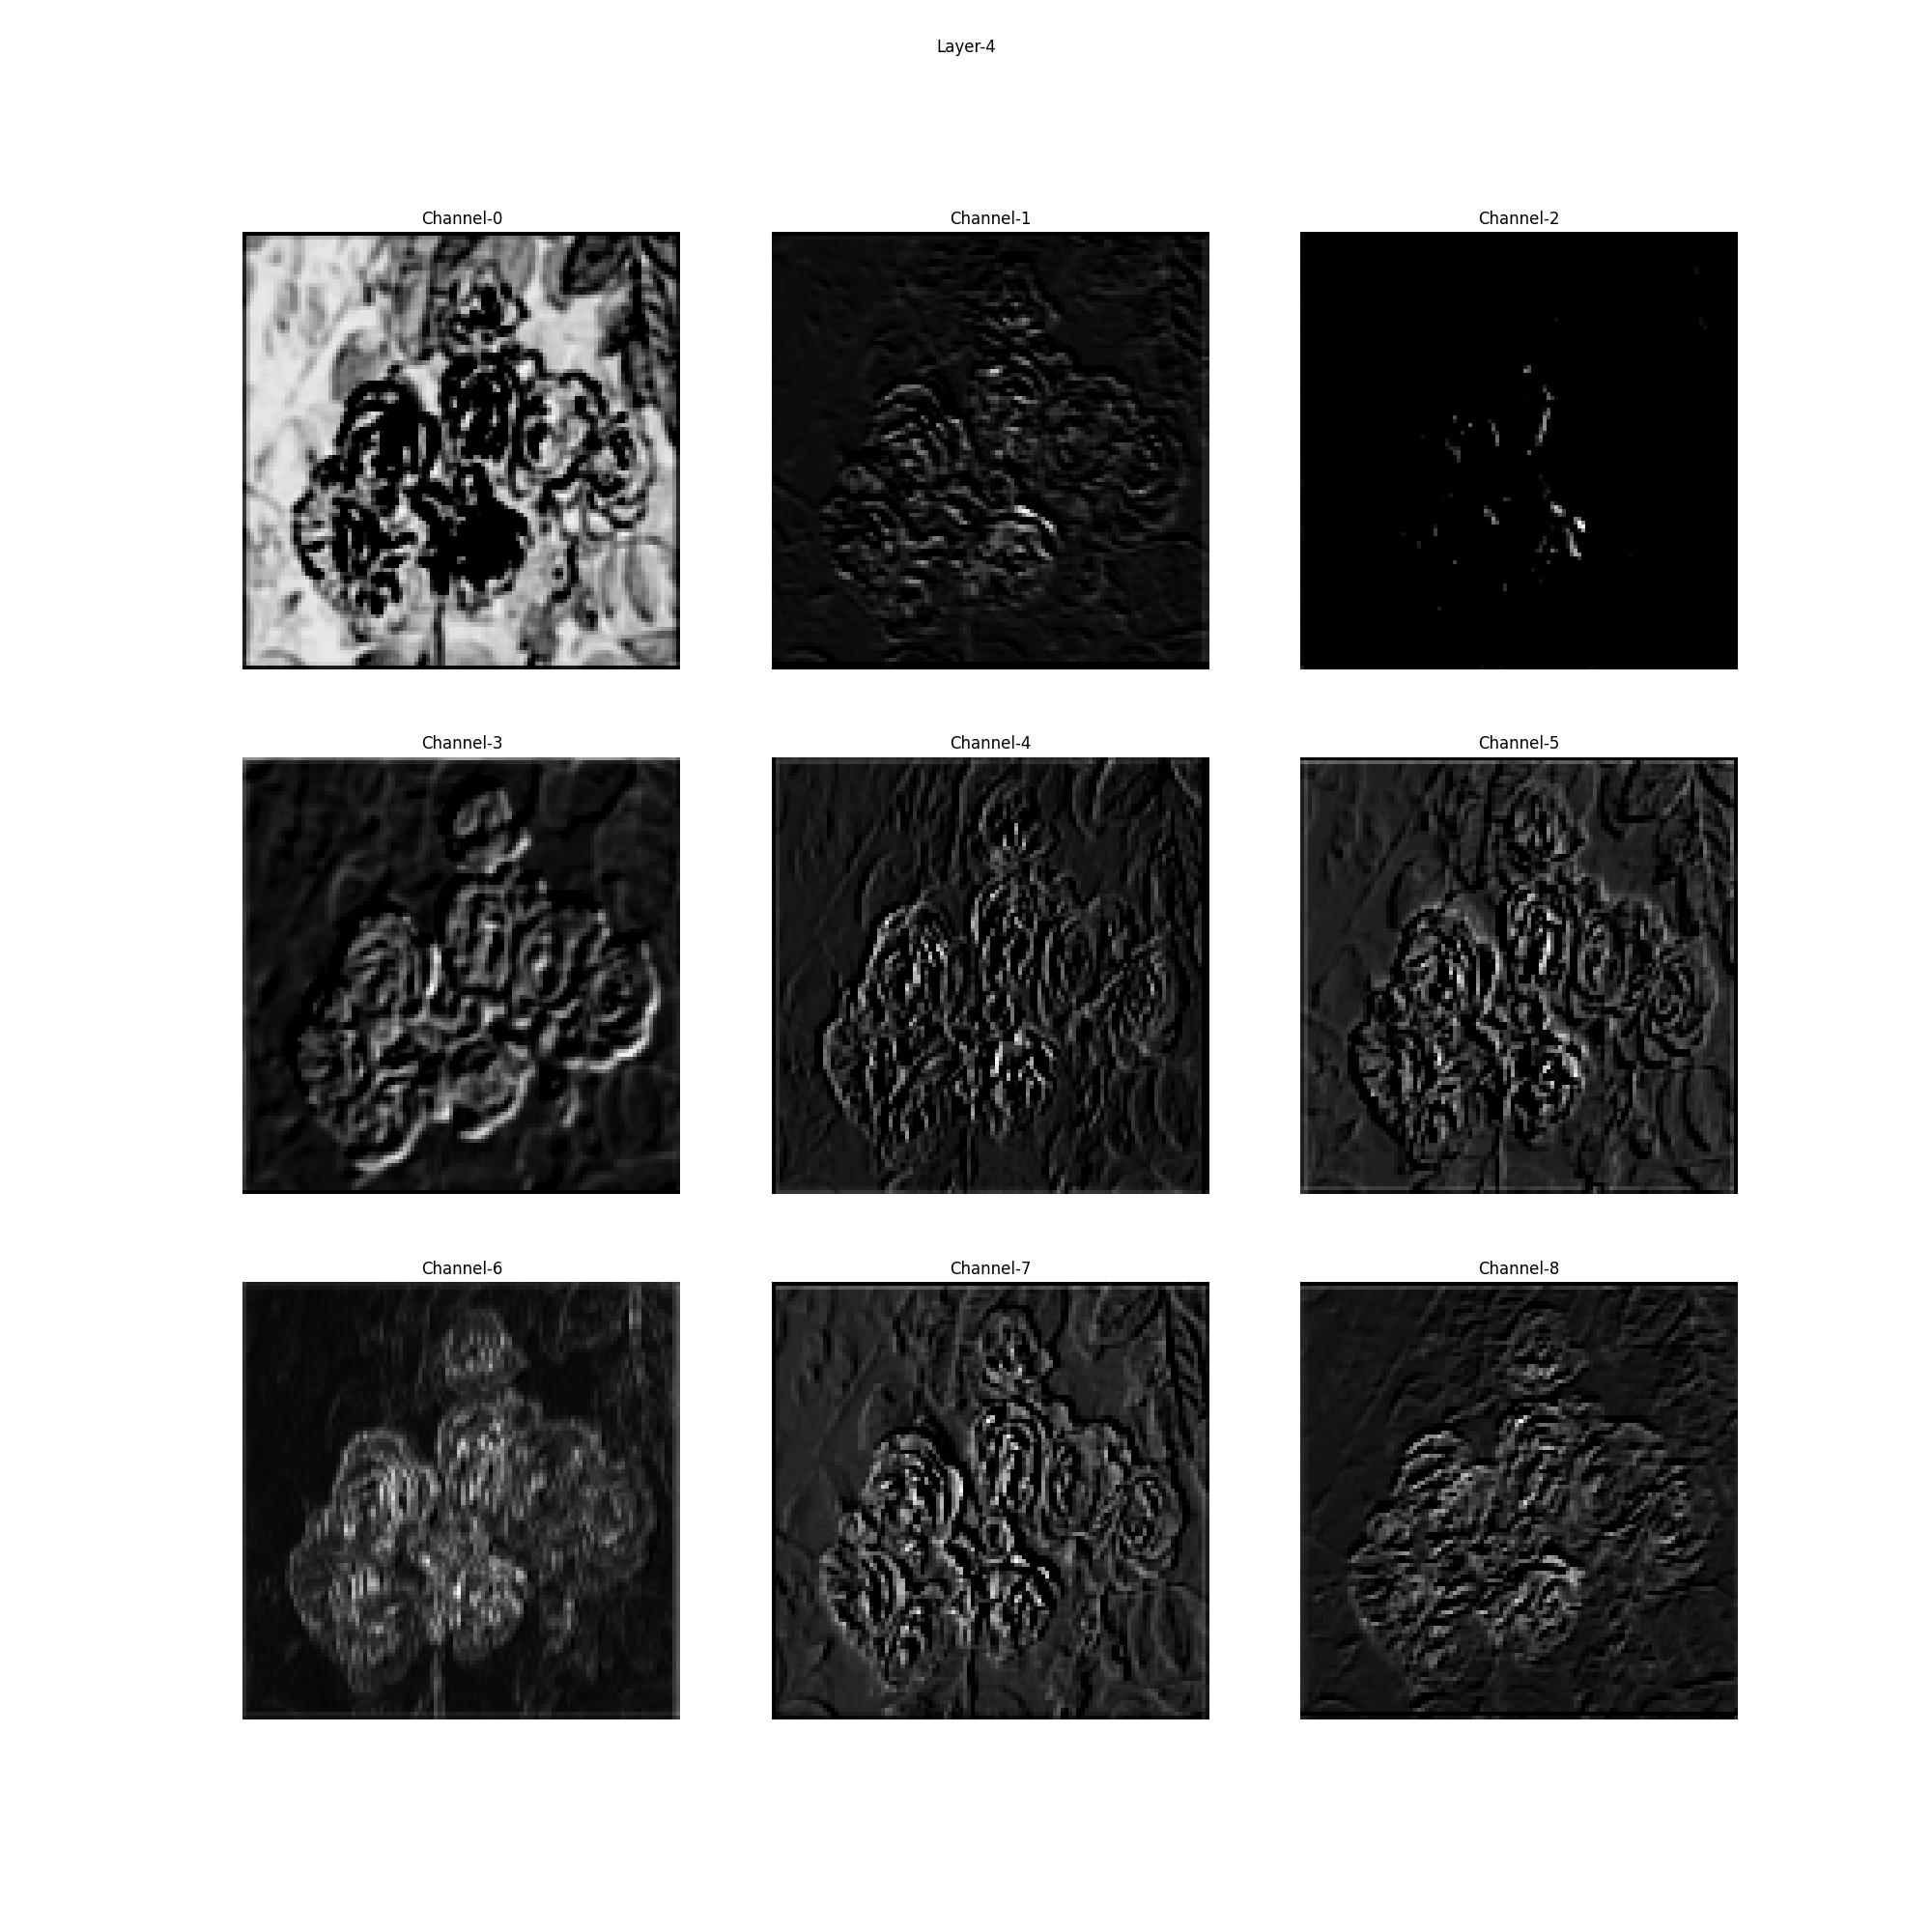
\includegraphics[width=0.33\textwidth]{Assignment-12/fig-4.jpg}
                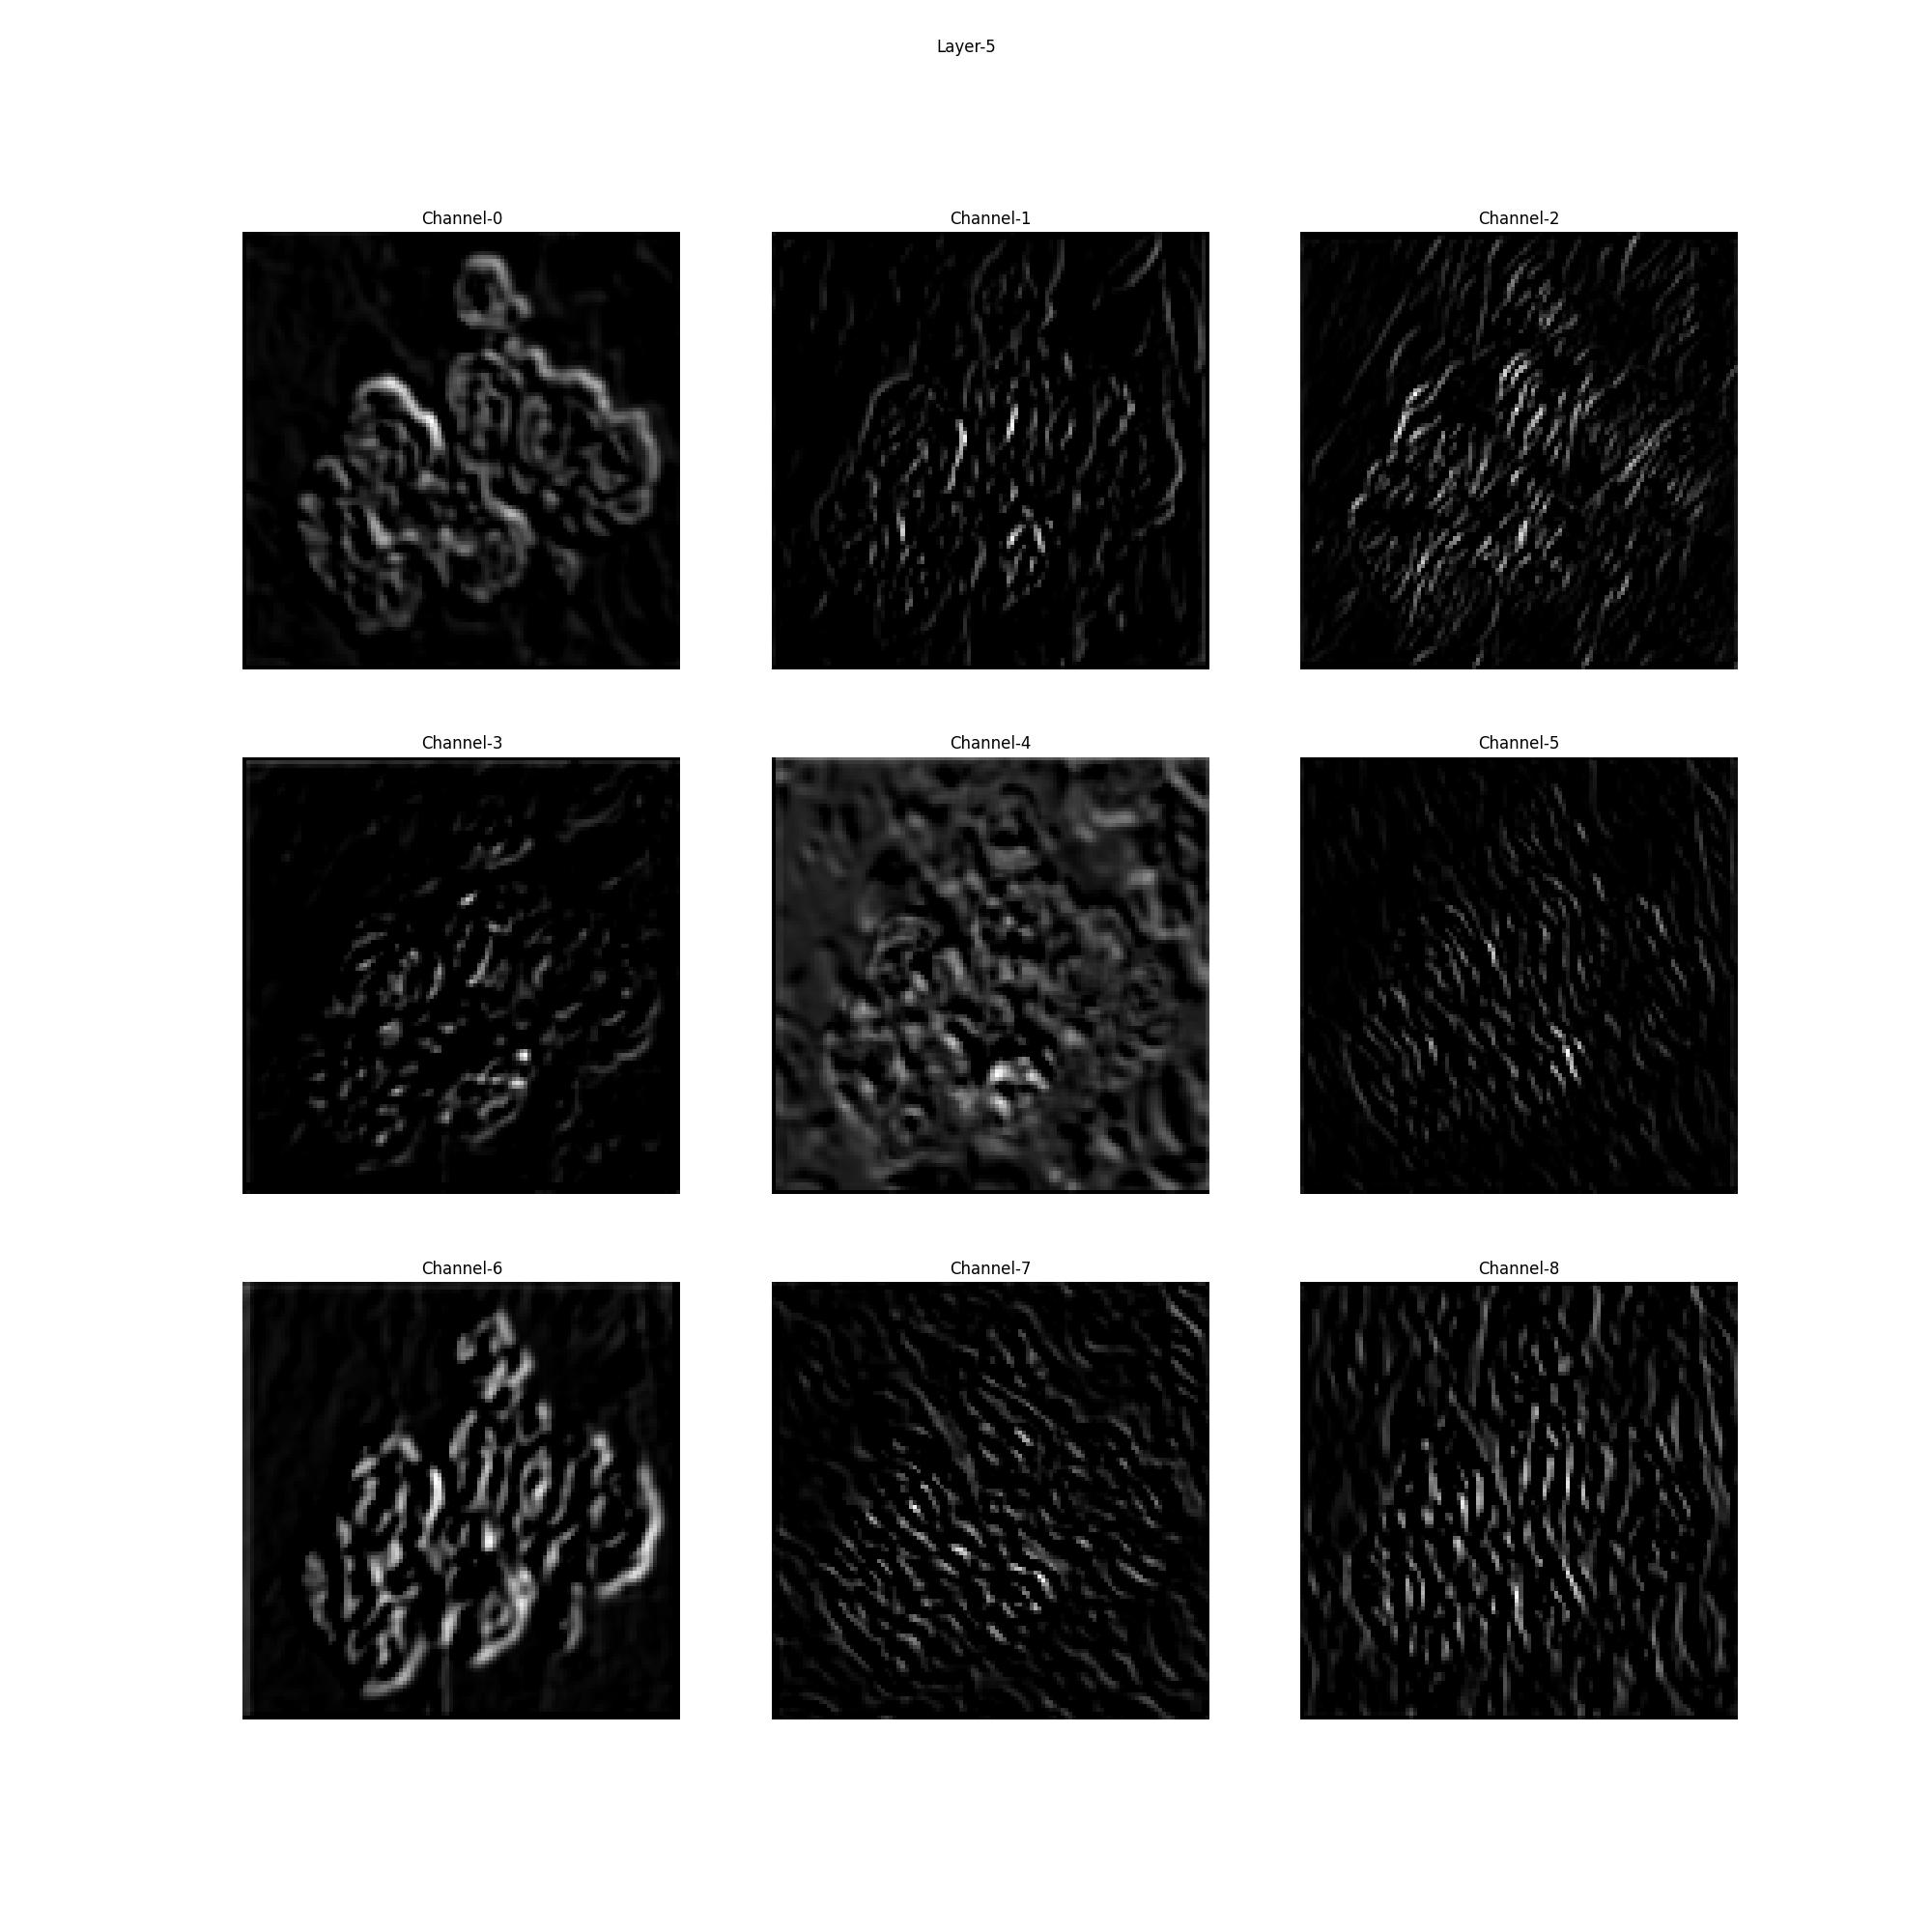
\includegraphics[width=0.33\textwidth]{Assignment-12/fig-5.jpg}
            \end{overprint}
            \begin{overprint}
                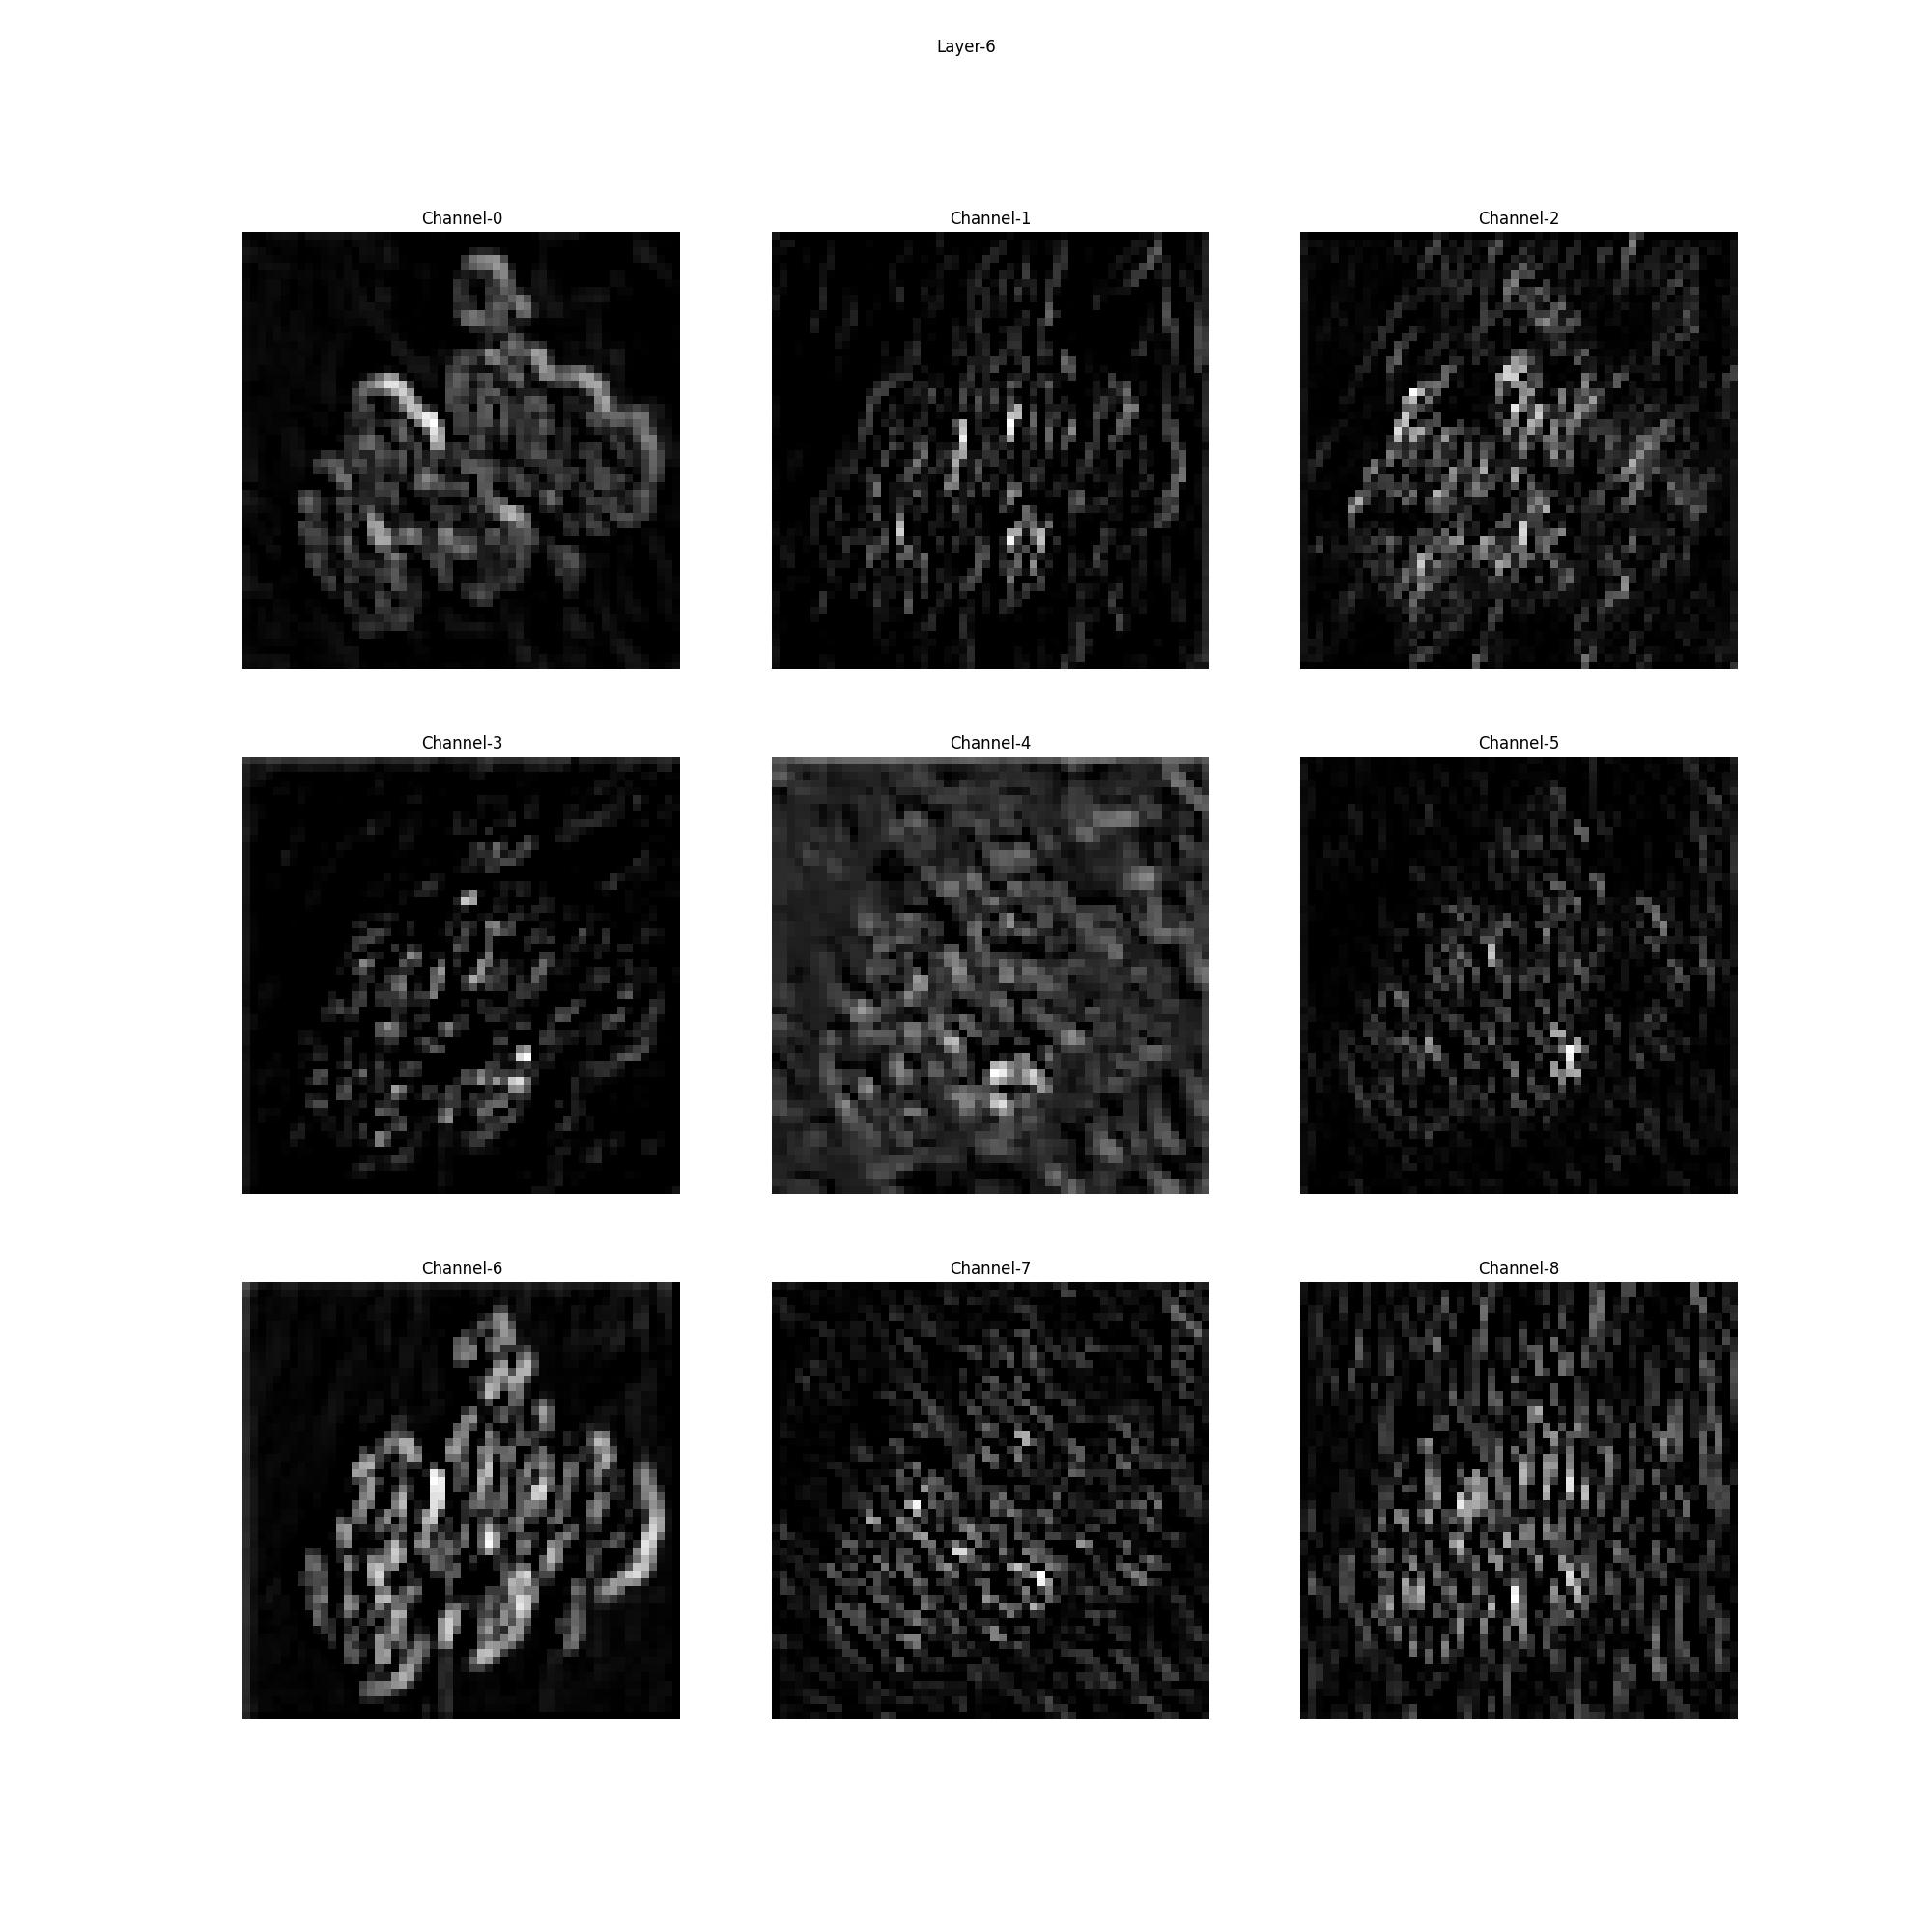
\includegraphics[width=0.33\textwidth]{Assignment-12/fig-6.jpg}
                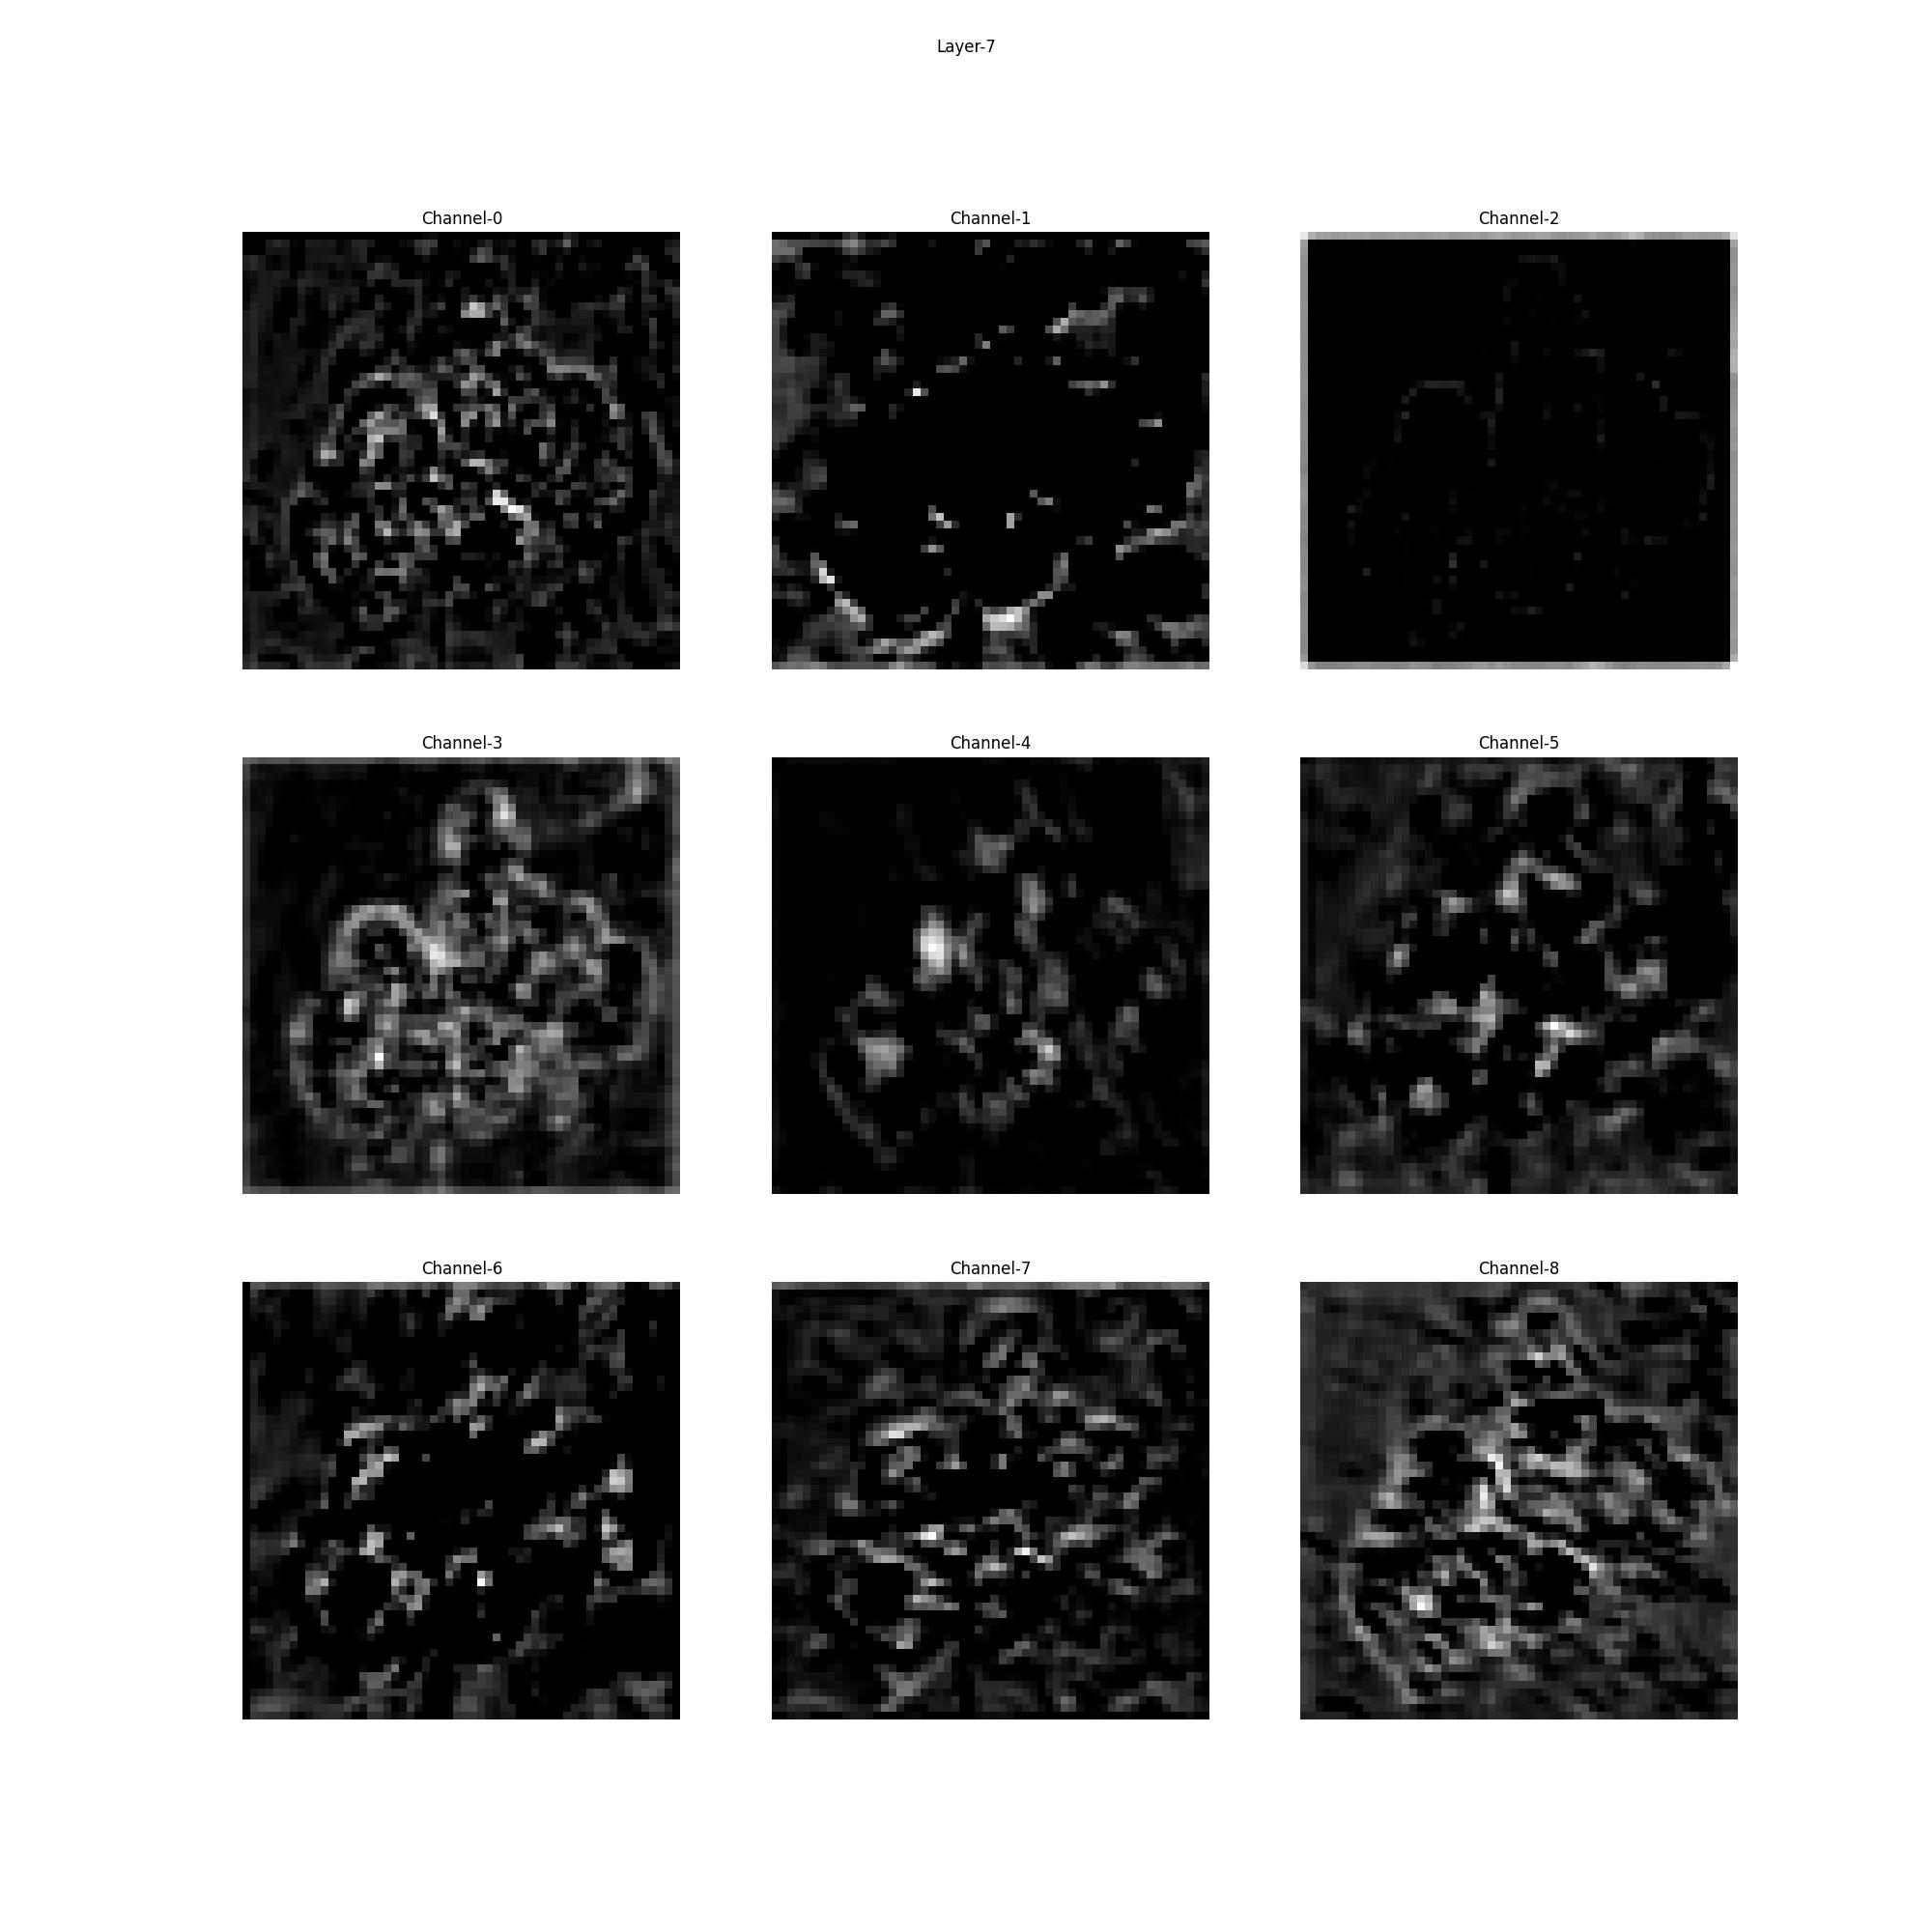
\includegraphics[width=0.33\textwidth]{Assignment-12/fig-7.jpg}
                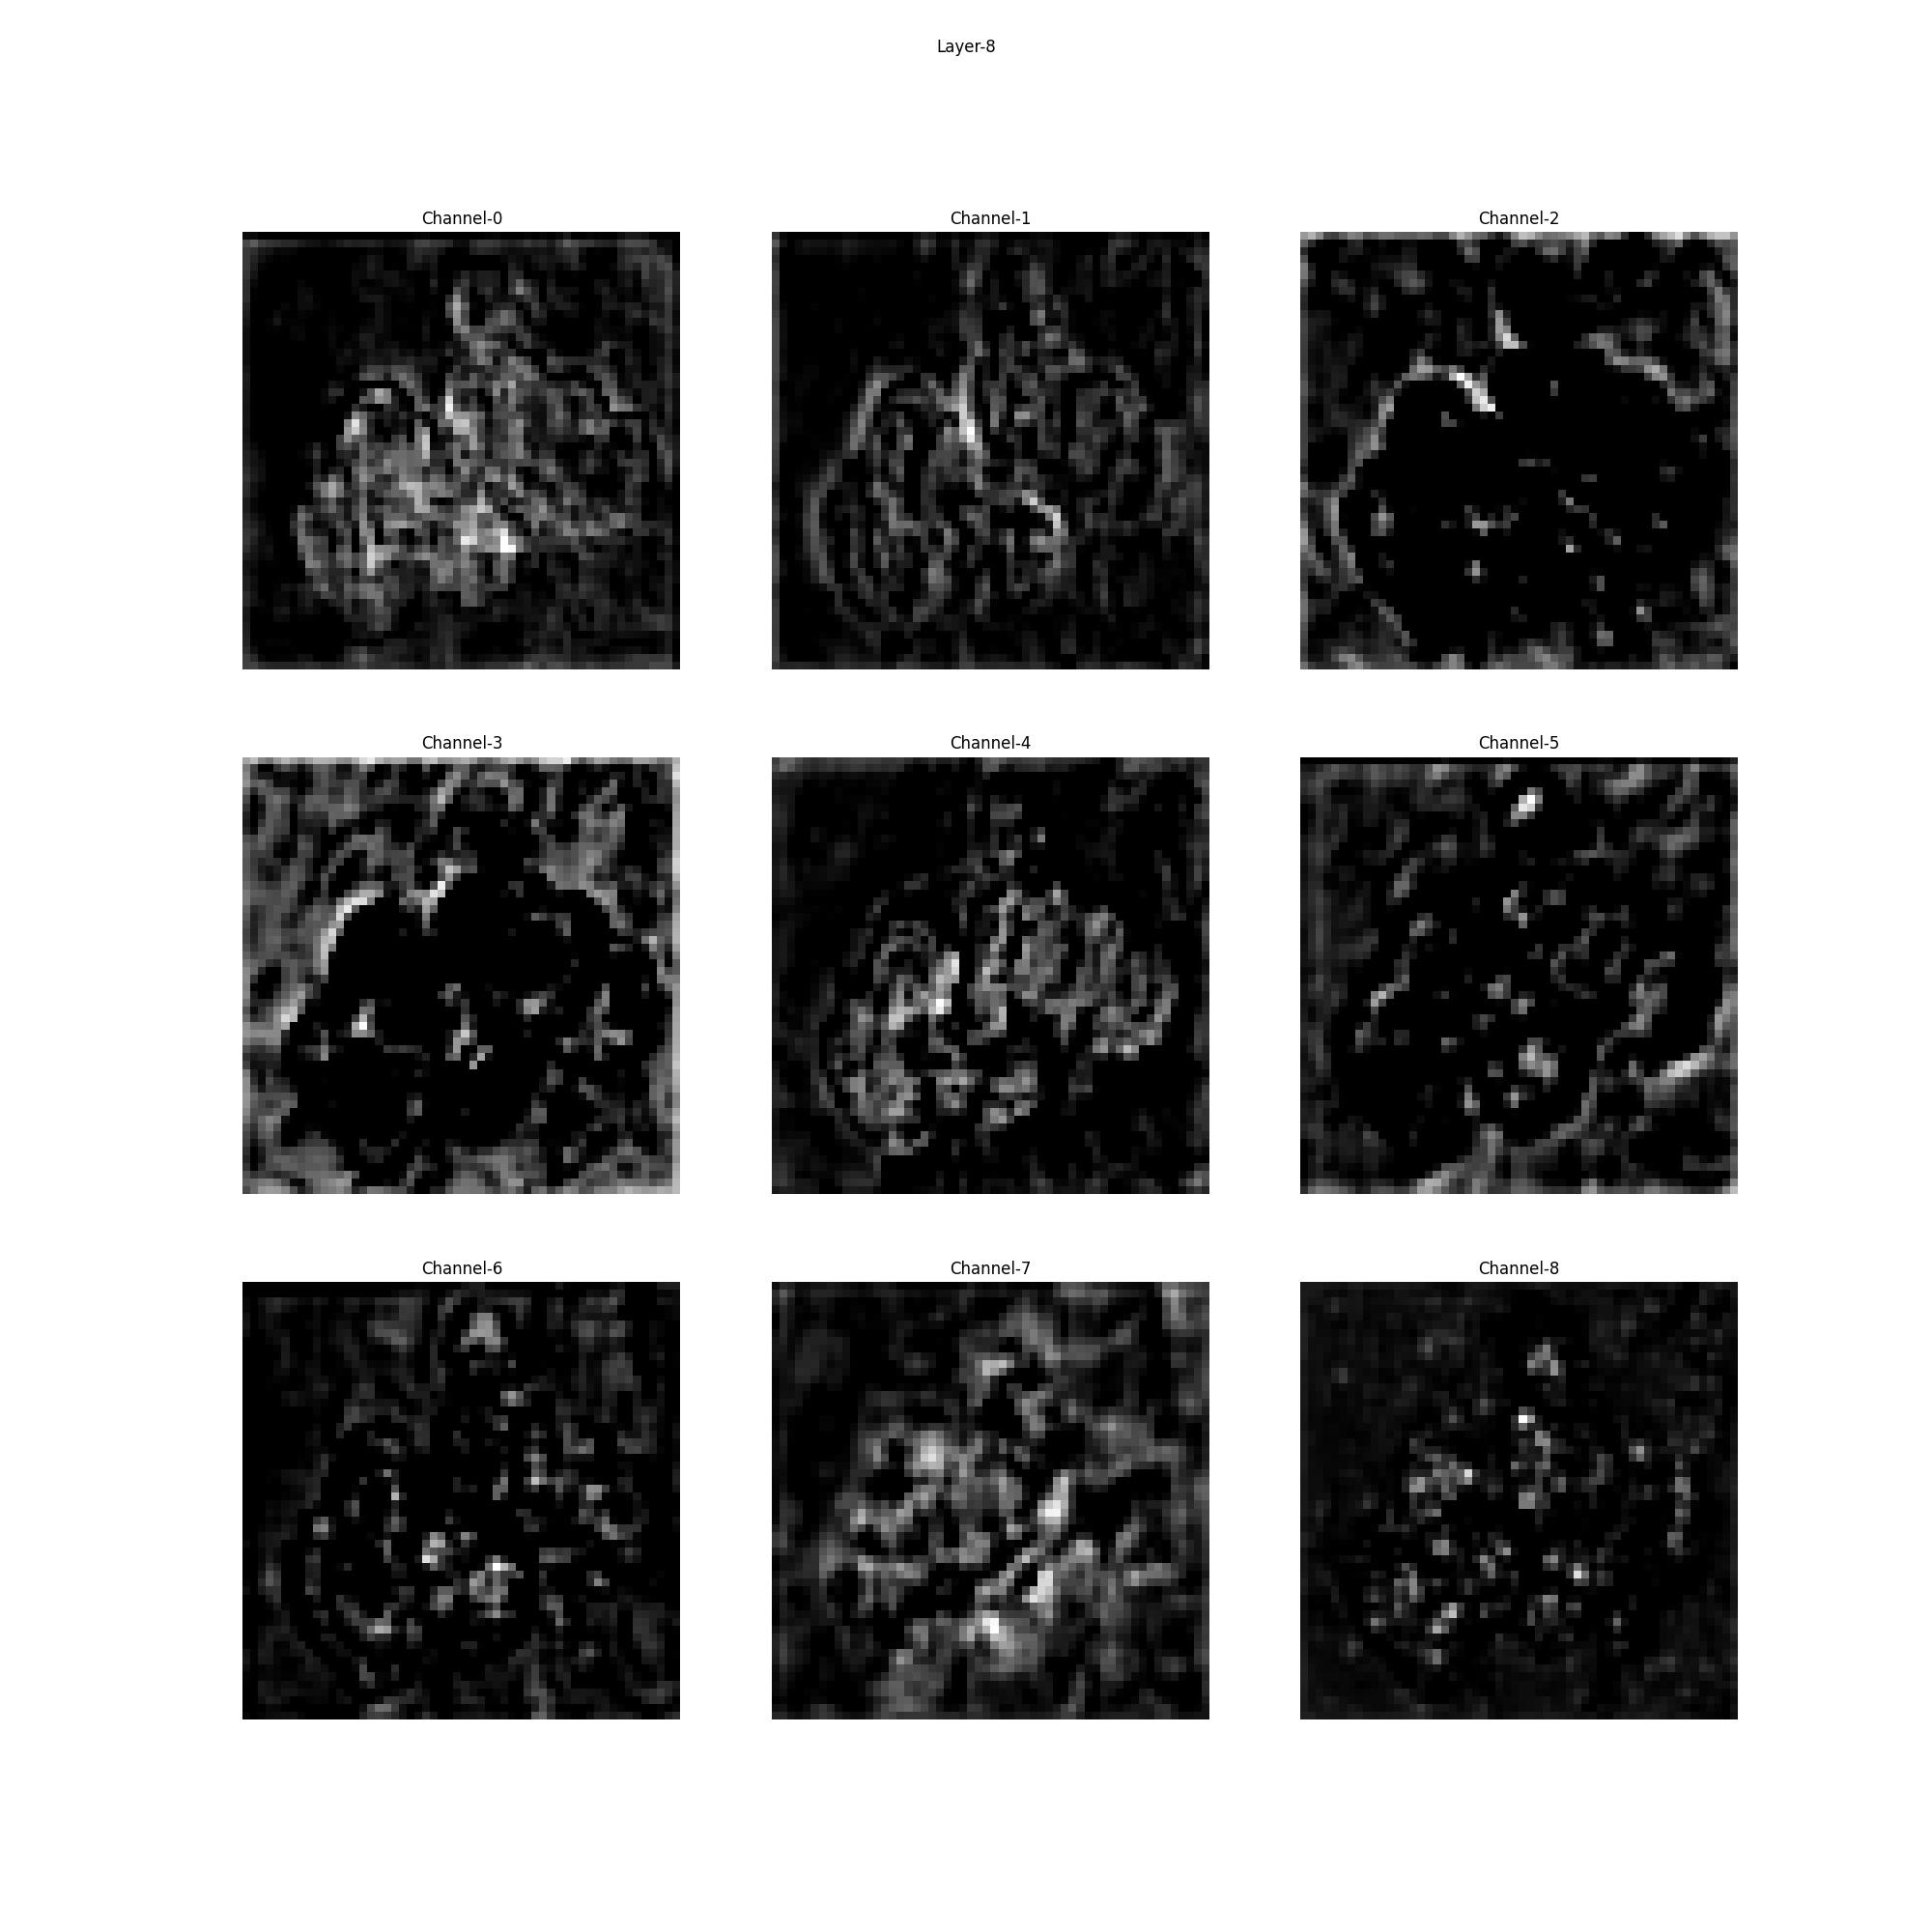
\includegraphics[width=0.33\textwidth]{Assignment-12/fig-8.jpg}
            \end{overprint}
            \begin{overprint}
                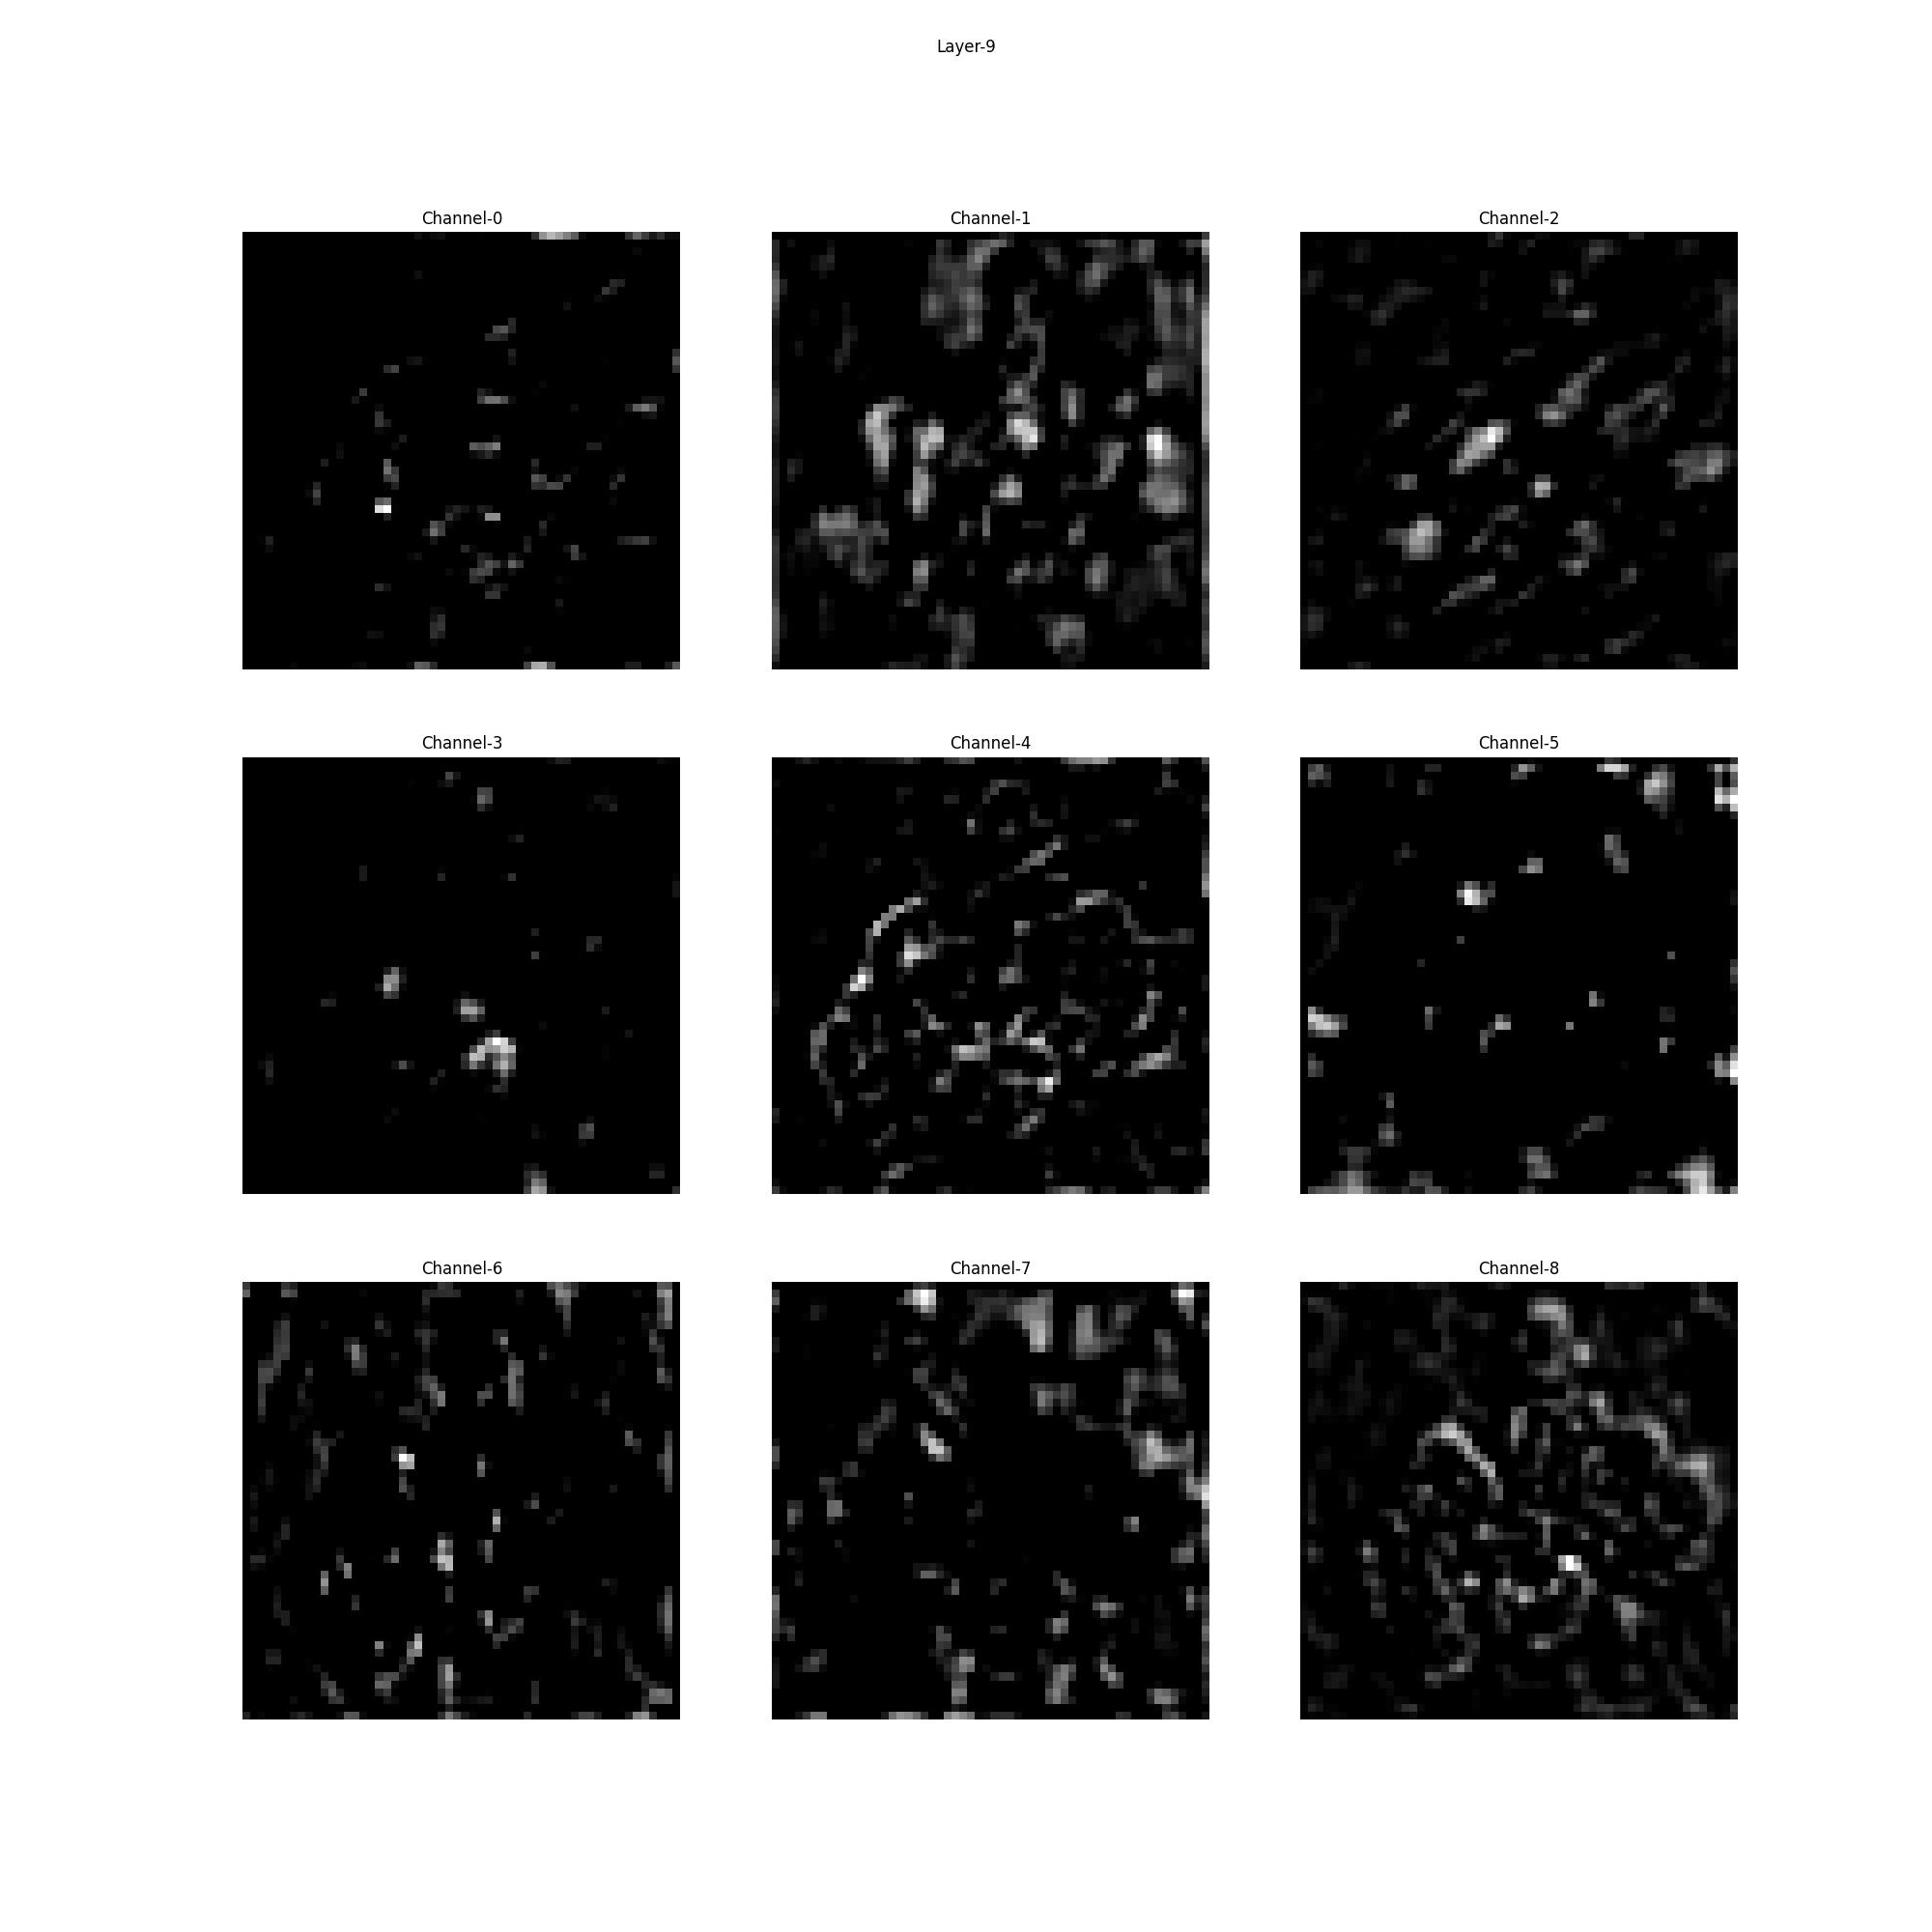
\includegraphics[width=0.33\textwidth]{Assignment-12/fig-9.jpg}
                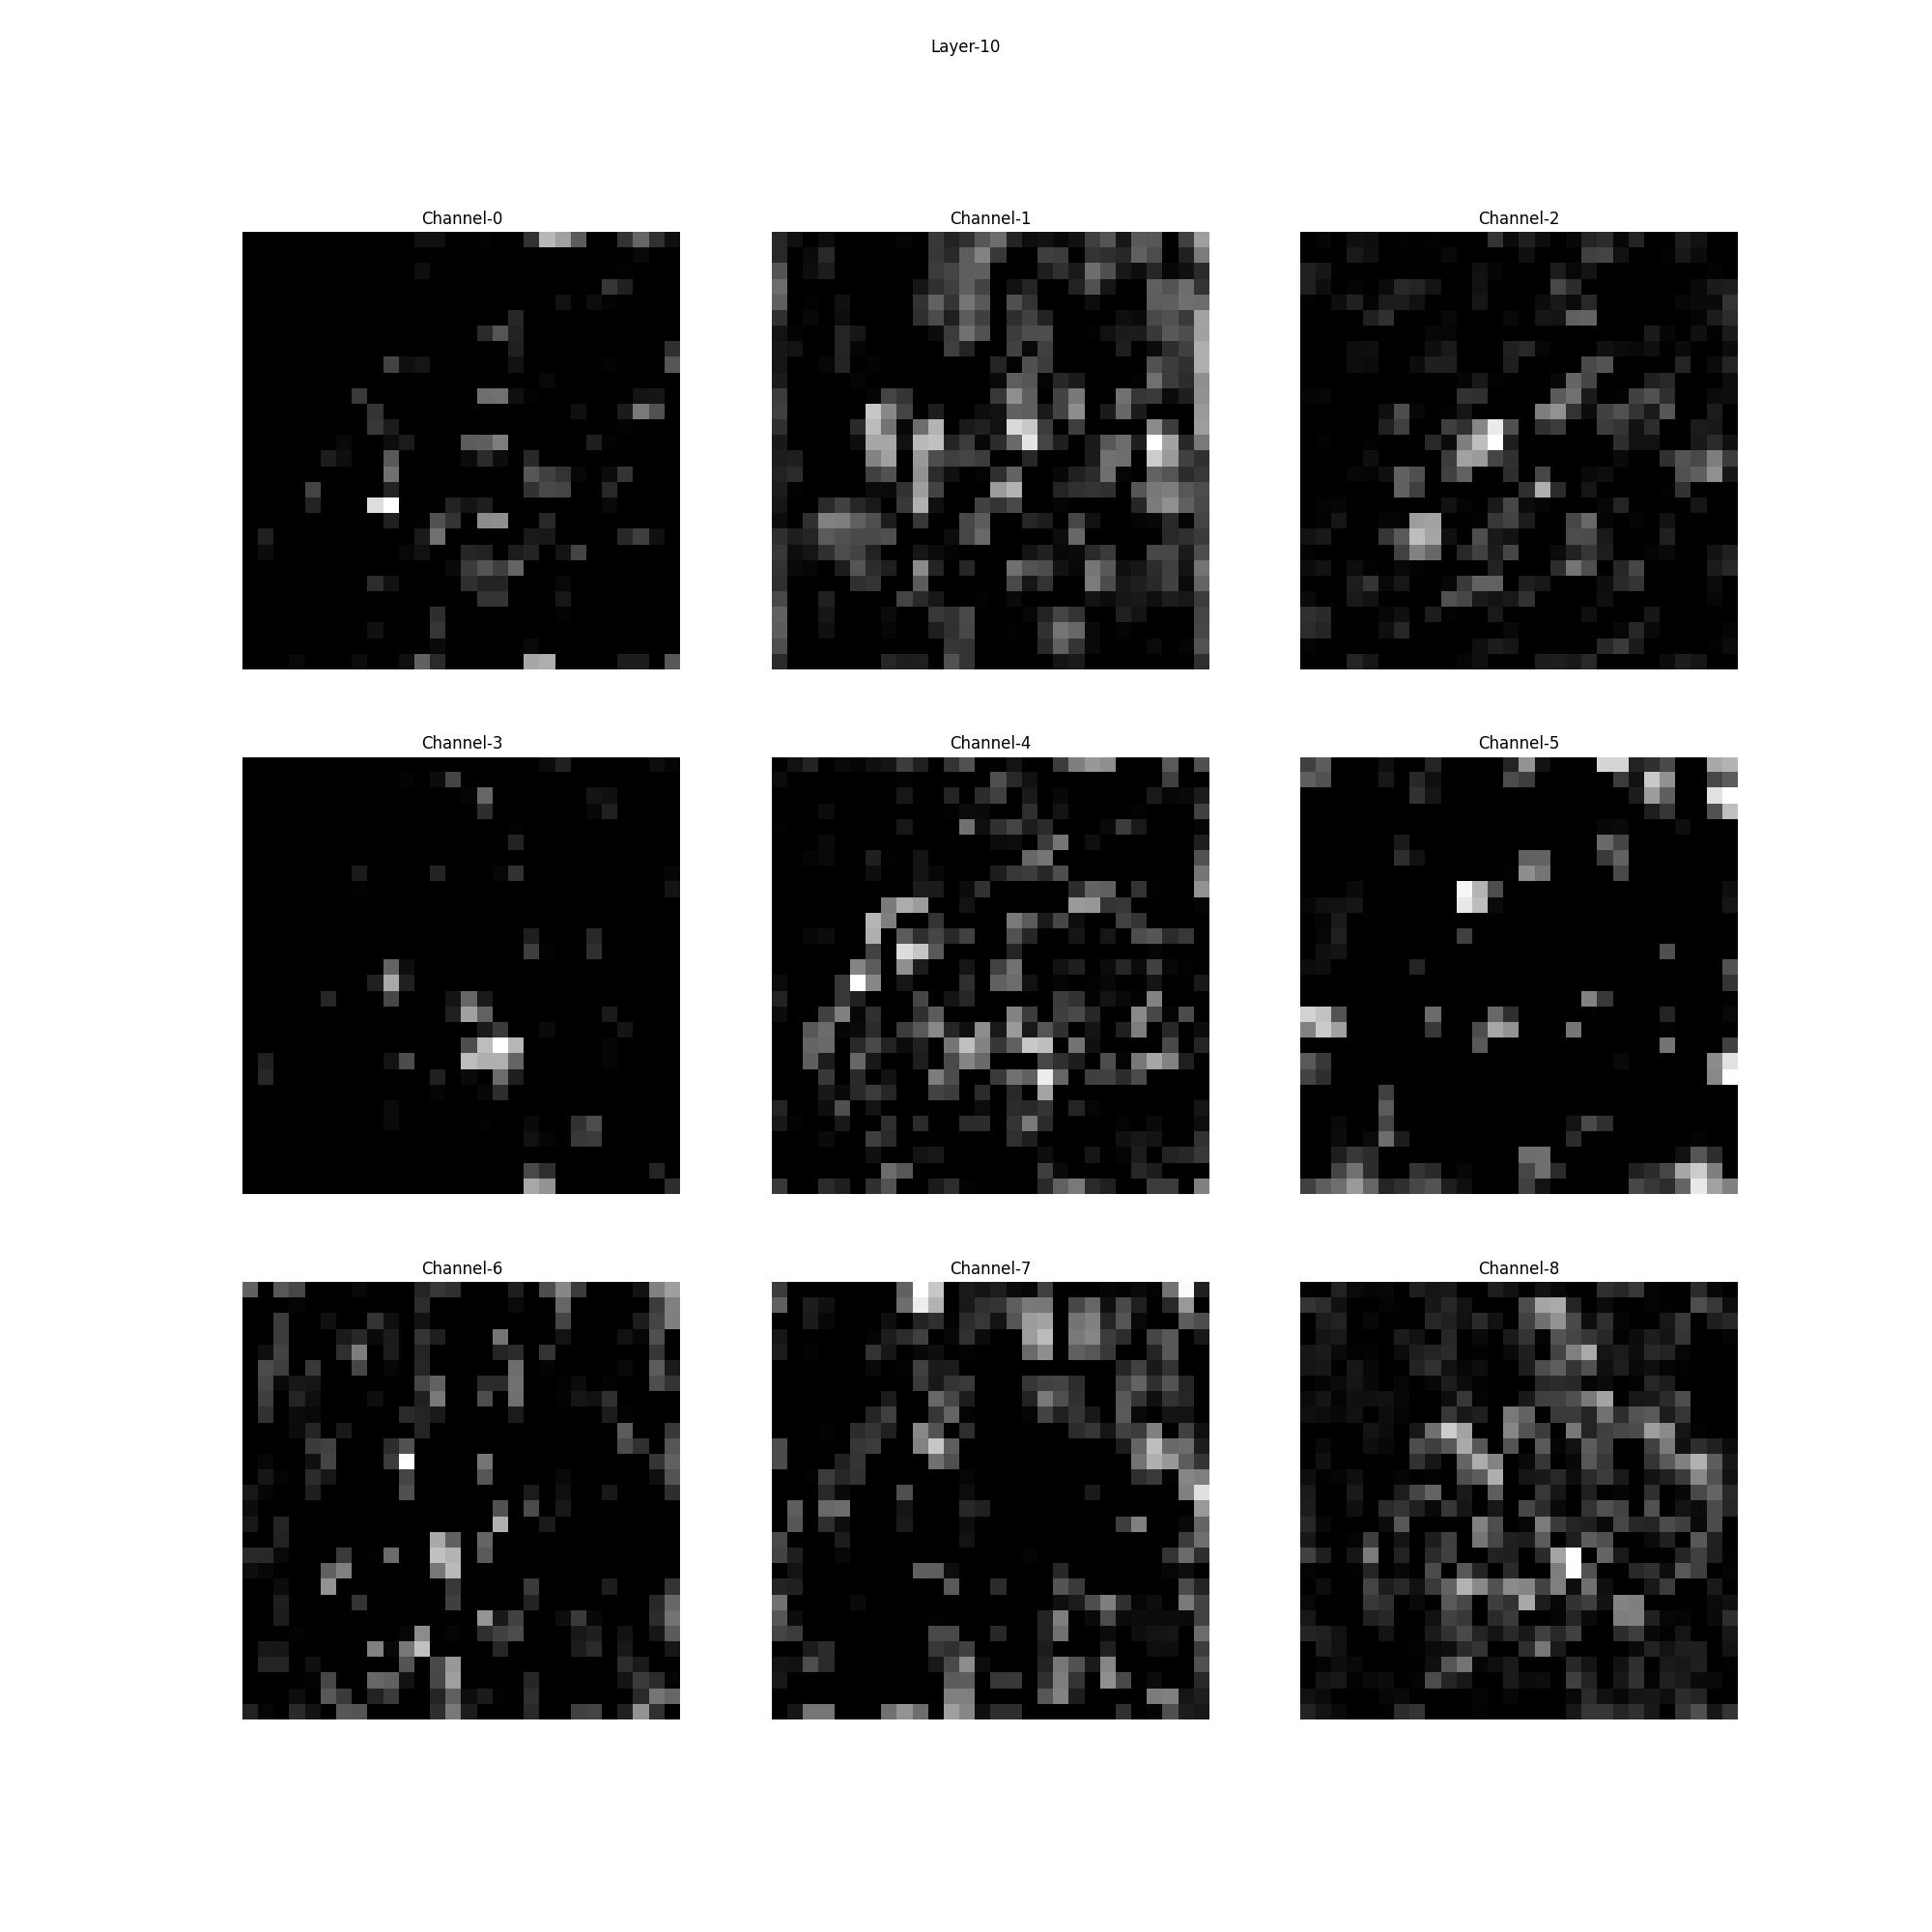
\includegraphics[width=0.33\textwidth]{Assignment-12/fig-10.jpg}
            \end{overprint}
            \caption{Input image, Output of Different Layers of VGG16 model from layer 1-10}
        \end{figure}
    }
}
% \pagebreak
\clearpage

%-----------------------Assignment-13-------------------------%
{
    \section{Assignment-13}
    \subsection{Introduction}
    \textbf {Problem: }
    Write a program to turn a JPEG image into a PNG image and vice-versa.\\
    \\
    \textbf{Solution: }
    Here we have to load a jpeg typed image at first, then we have to convert it to png and again, we have to load a png image and convert it to jpeg format. At the time time of conversion, we have to check the metadata of the header of the image and find the difference. So, we need two codes here for each of the conversion and showing the metadata of image header for better understanding. The codes, images and outputs are given below.\\
    
    \subsection{Required Software}
    Here we have to at first, install Pillow for image conversion and also for getting the metadata of the image header file. We specifically import the Image from PIL and PIL.ExifTags for the metadata extraction. We can also use imghdr which is very much helpful in showing the format of the image.\\
 
    \subsection{Procedure}
    \textbf{Step-1:}
    Install PILLOW and imghdr, import them in required program.\\
    \textbf{Step-2:}
    Show image type. (using imghdr.what()) \\
    \textbf{Step-3:}
    In code, read image of type jpeg or png. (usning Image.open())\\
    \textbf{Step-4:}
    Extract metadata from the image and save it in a dictionary. Then show the metadata in terminal. \\
    \textbf{Step-5:}
    Convert the image in png or jpeg format (using .save(), .covert()) and save it. \\  
    
    \subsection{Code}
    \lstset{style=mystyle}
    \begin{lstlisting}[language=Python, caption=Code for JPEG to PNG Image Conversion]
    from PIL import Image
    from PIL.ExifTags import TAGS 
    import imghdr
    
    def main():
        # path to the image or video
        img_path = './tower.jpg'
        print(img_path)
        print(imghdr.what(img_path))
    
        # read the image data using PIL
        image = Image.open(img_path)
        # print(image)
    
        # extract other basic metadata
        info_dict = {
            "Filename" : image.filename,
            "Image Size" : image.size,
            "Image Height" : image.height,
            "Image Width" : image.width,
            "Image Format" : image.format,
            "Image Mode" : image.mode,
            "Animated Image" : getattr(image, "is_animated", False),
            "Frames in Image" : getattr(image, "n_frames", 1)
        }
    
        # showing basic information
        for label, value in info_dict.items():
            print(f"{label:25}: {value}")
        
        # extract EXIF data
        exifdata = image.getexif()
    
        # iterating over all EXIF data fields
        for tag_id in exifdata:
            # get the tag name, instead of human unreadable tad id
            tag = TAGS.get(tag_id, tag_id)
            data = exifdata.get(tag_id)
            # decode bytes
            if isinstance(data, bytes):
                data = data.decode()
            print(f"{tag:25}: {data}")
        
        # jpg to png conversion
        image.save("tower.png")
        
    
    if __name__ == '__main__':
        main()
    
    \end{lstlisting}
    \\
    \lstset{style=mystyle}
    \begin{lstlisting}[language=Python, caption=Output of JPEG to PNG Image Conversion]
    ./tower.jpg
    jpeg
    Filename                 : ./tower.jpg
    Image Size               : (640, 480)
    Image Height             : 480
    Image Width              : 640
    Image Format             : JPEG
    Image Mode               : RGB
    Animated Image           : False
    Frames in Image          : 1
    \end{lstlisting}
    \\
    \lstset{style=mystyle}
    \begin{lstlisting}[language=Python, caption=Code for PNG to JPEG Image Conversion]
    from PIL import Image
    from PIL.ExifTags import TAGS 
    import imghdr
    
    def main():
        # path to the image or video
        img_path = './tower.png'
        print(img_path)
        print(imghdr.what(img_path))
    
        # read the image data using PIL
        image = Image.open(img_path)
        print(image)
    
        # extract other basic metadata
        info_dict = {
            "Filename" : image.filename,
            "Image Size" : image.size,
            "Image Height" : image.height,
            "Image Width" : image.width,
            "Image Format" : image.format,
            "Image Mode" : image.mode,
            "Animated Image" : getattr(image, "is_animated", False),
            "Frames in Image" : getattr(image, "n_frames", 1)
        }
    
        # showing basic information
        for label, value in info_dict.items():
            print(f"{label:25}: {value}")
        
        # extract EXIF data
        exifdata = image.getexif()
    
        # iterating over all EXIF data fields
        for tag_id in exifdata:
            # get the tag name, instead of human unreadable tad id
            tag = TAGS.get(tag_id, tag_id)
            data = exifdata.get(tag_id)
            # decode bytes
            if isinstance(data, bytes):
                data = data.decode()
            print(f"{tag:25}: {data}")
        
        # jpg to png conversion
        image2 = image.convert('RGB')
        image2.save("tower2.jpeg")
    
    if __name__ == '__main__':
        main()

    \end{lstlisting}
    \\
    \lstset{style=mystyle}
    \begin{lstlisting}[language=Python, caption=Output of PNG to JPEG Image Conversion]
    ./tower.png
    png
    Filename                 : ./tower.png
    Image Size               : (640, 480)
    Image Height             : 480
    Image Width              : 640
    Image Format             : PNG
    Image Mode               : RGB
    Animated Image           : False
    Frames in Image          : 1
    \end{lstlisting}
    \\
    \subsection{Result & Discussion}
    Here in the output, we can see that the data is showing accordingly to the result. No inconsistency or error is observed. The input and output images are given below accordingly.

    \begin{figure}[htp]
        \begin{overprint}
            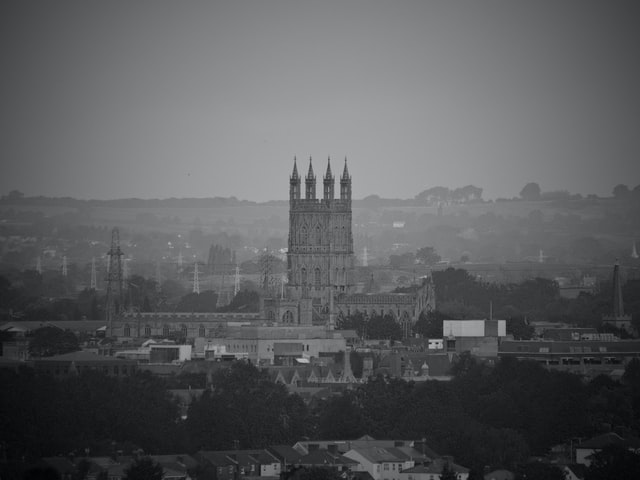
\includegraphics[width=0.33\textwidth]{Assignment-13/tower.jpg}
            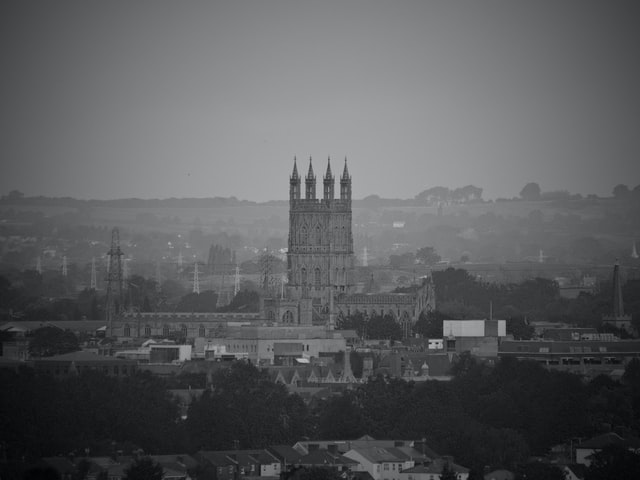
\includegraphics[width=0.33\textwidth]{Assignment-13/tower.png}
            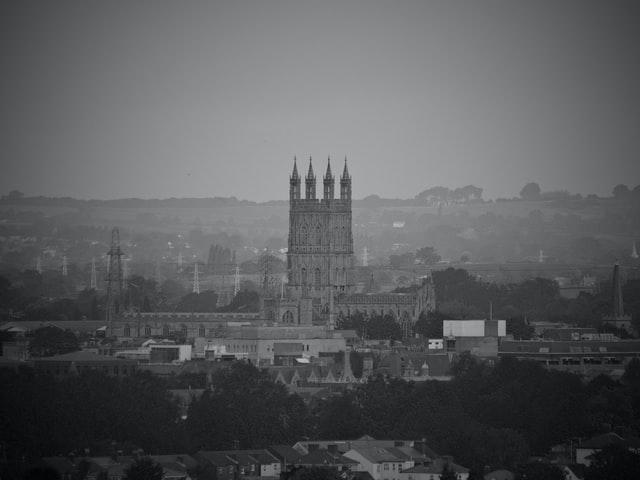
\includegraphics[width=0.33\textwidth]{Assignment-13/tower2.jpeg}
        \end{overprint}
        \caption{Input image of jpeg to png image conversion, Output image of jpeg to png image conversion and input image of png to jpeg image conversion, Output image of png to jpeg image conversion}
    \end{figure}
}
% \pagebreak
\clearpage

%-----------------------Assignment-14-------------------------%
{
    \section{Assignment-14}
    \subsection{Introduction}
    \textbf {Problem: }
    Write a program to perform JPEG compression on frequency domain.\\
    \\
    \textbf{Solution: }
    Here we have to perform JPEG compression on frequency domain. It may be noted here that if we do JPEG compression based on frequency domain, the dimension of image is not changed, rather the size of image is changed. This happens because as we are compressing the image based on the frequency, the highest frequencies are kept in the image and other lower frequencies are cut off. The phrase cut off means that frequencies energy becomes zero. So no information of that lower frequencies are saved. And we call that lower frequency as noise. Here we have do the same things. The code for image compression and its outcome is given below accordingly.\\
    \\
    \subsection{Required Software}
    Here for image compression, we have to use numpy, matplotlib and opencv(cv2) libraries for the code. These libraries are enough for our workings. We use matplotlib.pyplot for image taking input image and save output images, opencv(cv2) for image conversion and numpy for all other calculation.\\
    
    \subsection{Procedure}
    \textbf{Step-1:}
    Install numpy, matplotlib and opencv and import them in required program.\\
    \textbf{Step-2:}
    Read image (using plt.imread()) and convert it to grayscale (using cv2.cvtColor()) \\
    \textbf{Step-3:}
    Fourier transform the image and sort it by highest magnitude. \\
    \textbf{Step-4:}
    Find out the threshold for compressing the image. \\
    \textbf{Step-5:}
    Find out the indices of small frequency. \\
    \textbf{Step-6:}
    Threshold the small indices. \\
    \textbf{Step-7:}
    Compressed the image by Inverse Fourier Transform. \\
    \textbf{Step-8:}
    Save the images and plot them. \\
    
    \subsection{Code}
    \lstset{style=mystyle}
    \begin{lstlisting}[language=Python, caption=Code for Image Compression on Frequency Domain]
    import matplotlib.pyplot as plt
    import numpy as np
    import cv2 as cv
    
    def main():
        img_path = './trees_in_water.jpg'
        print(img_path)
    
        img_rgb = plt.imread(img_path)
        print(img_rgb.shape)
    
        img_gray = cv.cvtColor(img_rgb, cv.COLOR_RGB2GRAY)
        print(img_gray.shape)
        cnt = 0
        # plt.imshow(img_gray, cmap='gray')
        # plt.savefig('fig-0.jpg')
        # plt.show()
        plt.imsave('./fig-' + str(cnt) + '.jpg', img_gray, format='jpg', cmap='gray')
    
        img_set = [img_gray]
        img_title = ['Grayscale']
    
        ft = np.fft.fft2(img_gray)
        ftSort = np.sort(np.abs(ft.reshape(-1))) # sort by highest magnitude
    
        cnt = 0
        # Zero out all the small co-efficients and inverse transformation
        for keep in (0.75 , 0.5 , 0.1 , 0.05 , 0.01, 0.001 , 0.0001):
            thresh = ftSort[int(np.floor((1-keep)*len(ftSort)))]
            ind = np.abs(ft) > thresh           # find small indices
            Atlow = ft * ind                    # threshold small indices
            ftlow = np.fft.ifft2(Atlow).real    # compressed image
            img_set.append(ftlow)
            img_title.append('Image at ' + str(keep*100) + '%' + ' compression')
            cnt += 1
            plt.imsave('./fig-' + str(cnt) + '.jpg', ftlow, format='jpg', cmap='gray')
            print(ftlow.shape)
    
        img_plot(img_set, img_title)
    
    def img_plot(img_set, img_title):
        n = len(img_set)
        plt.figure(figsize = (20, 20))
        for i in range(n):
            plt.subplot(2, 4, i+1)
            plt.imshow(img_set[i], cmap='gray')
            plt.title(img_title[i])
            
        plt.savefig('output.jpg')
        plt.show()
    
    if __name__ == '__main__':
        main()
    
    # image save option
    # import matplotlib.image as mpimg
    
    # img = mpimg.imread("src.png")
    # mpimg.imsave("out.png", img)

    \end{lstlisting}
    \\
    
    \subsection{Result & Discussion}
    Here in the output, we can see that the size of image changes with the compression percentage but the height and width remains same. Sometimes the size is increasing and other times, it is decreasing. In the output figure, at first the grayscale image is shown which is used for compression. It has size of 1.3 MB (1,324,171 bytes). The 1st output image of 75\% image compression has size of 1.3 MB (1,335,669 bytes). So, the size has increased. The 2nd output image of 50\% image compression has size of 1.3 MB (1,323,616 bytes). So, the size has decreased. The 3rd output image of 10\% image compression has size of 1.5 MB (1,489,565 bytes). So, the size has increased. The 4th output image of 5\% image compression has size of 1.5 MB (1,507,115 bytes). So, the size has increased. The 5th output image of 1\% image compression has size of 1.1 MB (1,114,207 bytes). So, the size has decreased. The 6th output image of 0.1\% image compression has size of 766.9 kB (766,909 bytes). So, the size has decreased. The 7th output image of 0.01\% image compression has size of 636.4 kB (636,408 bytes). So, the size has decreased. This has happened because perhaps when the compression technique is applied, as for unique values, the storing values increases which results in increasing the size of output image. 
    
    \begin{figure}[htp]
        \begin{overprint}
            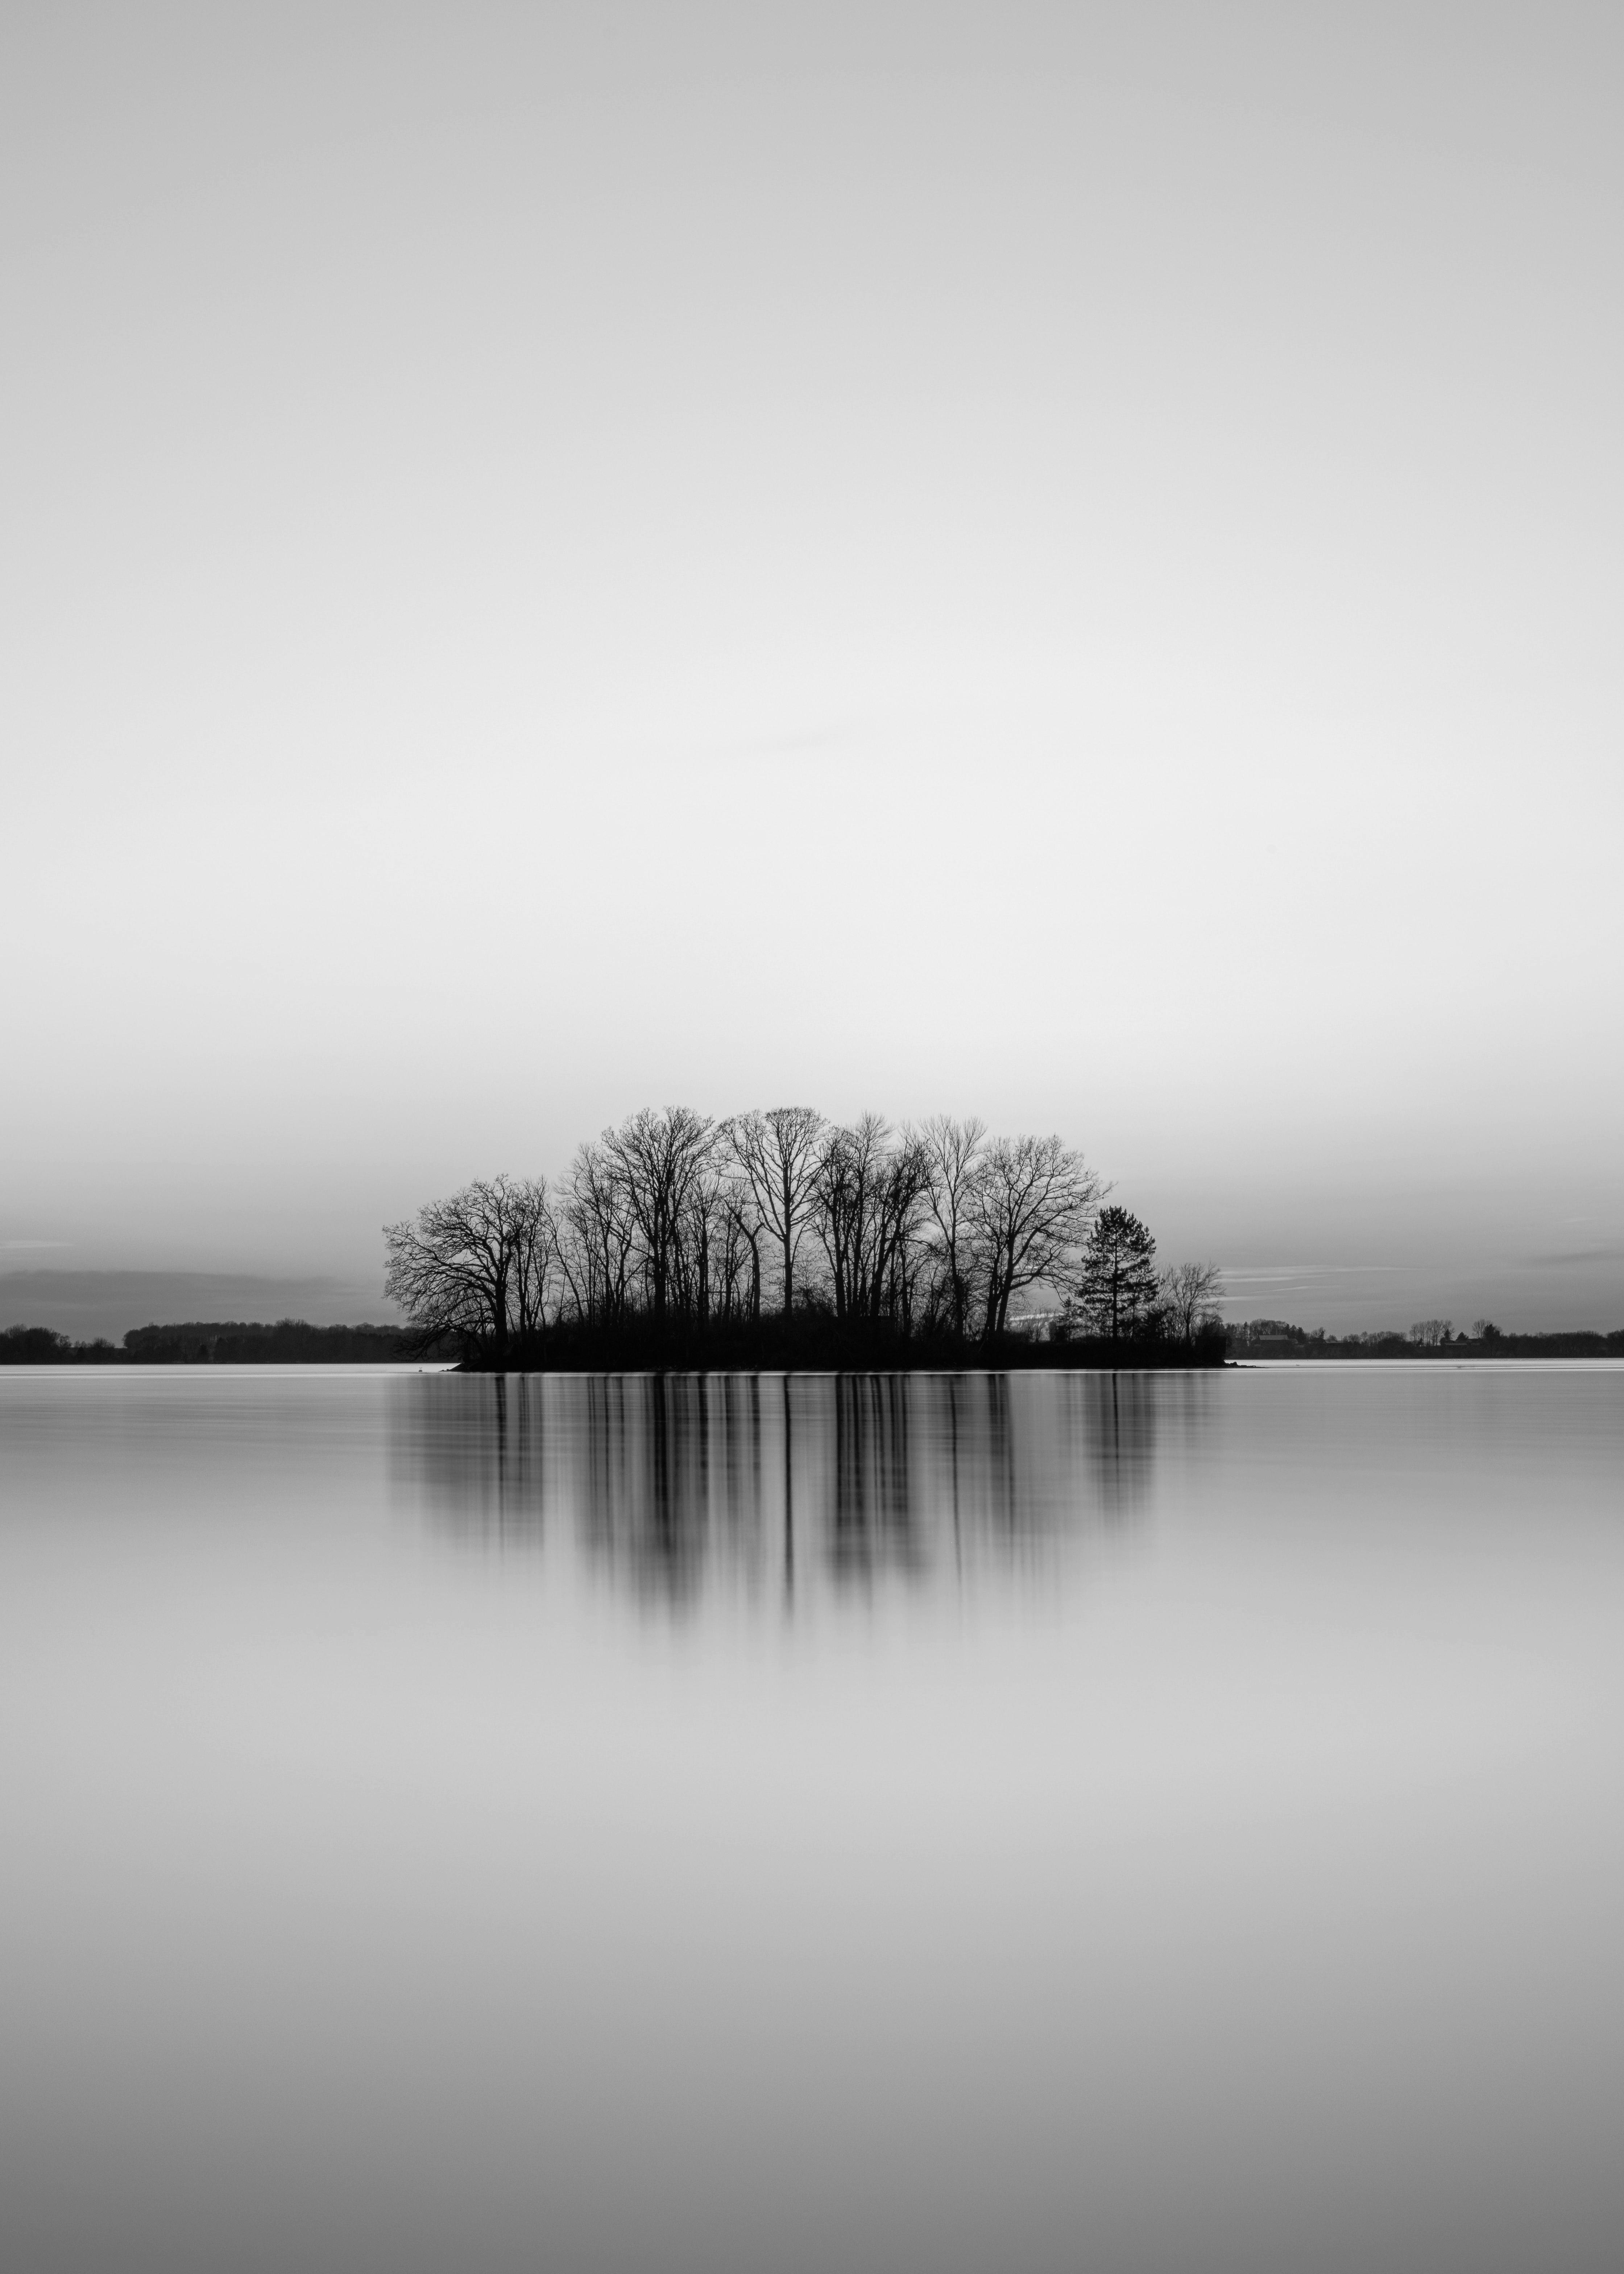
\includegraphics[width=0.33\textwidth]{Assignment-14/fig-0.jpg}
            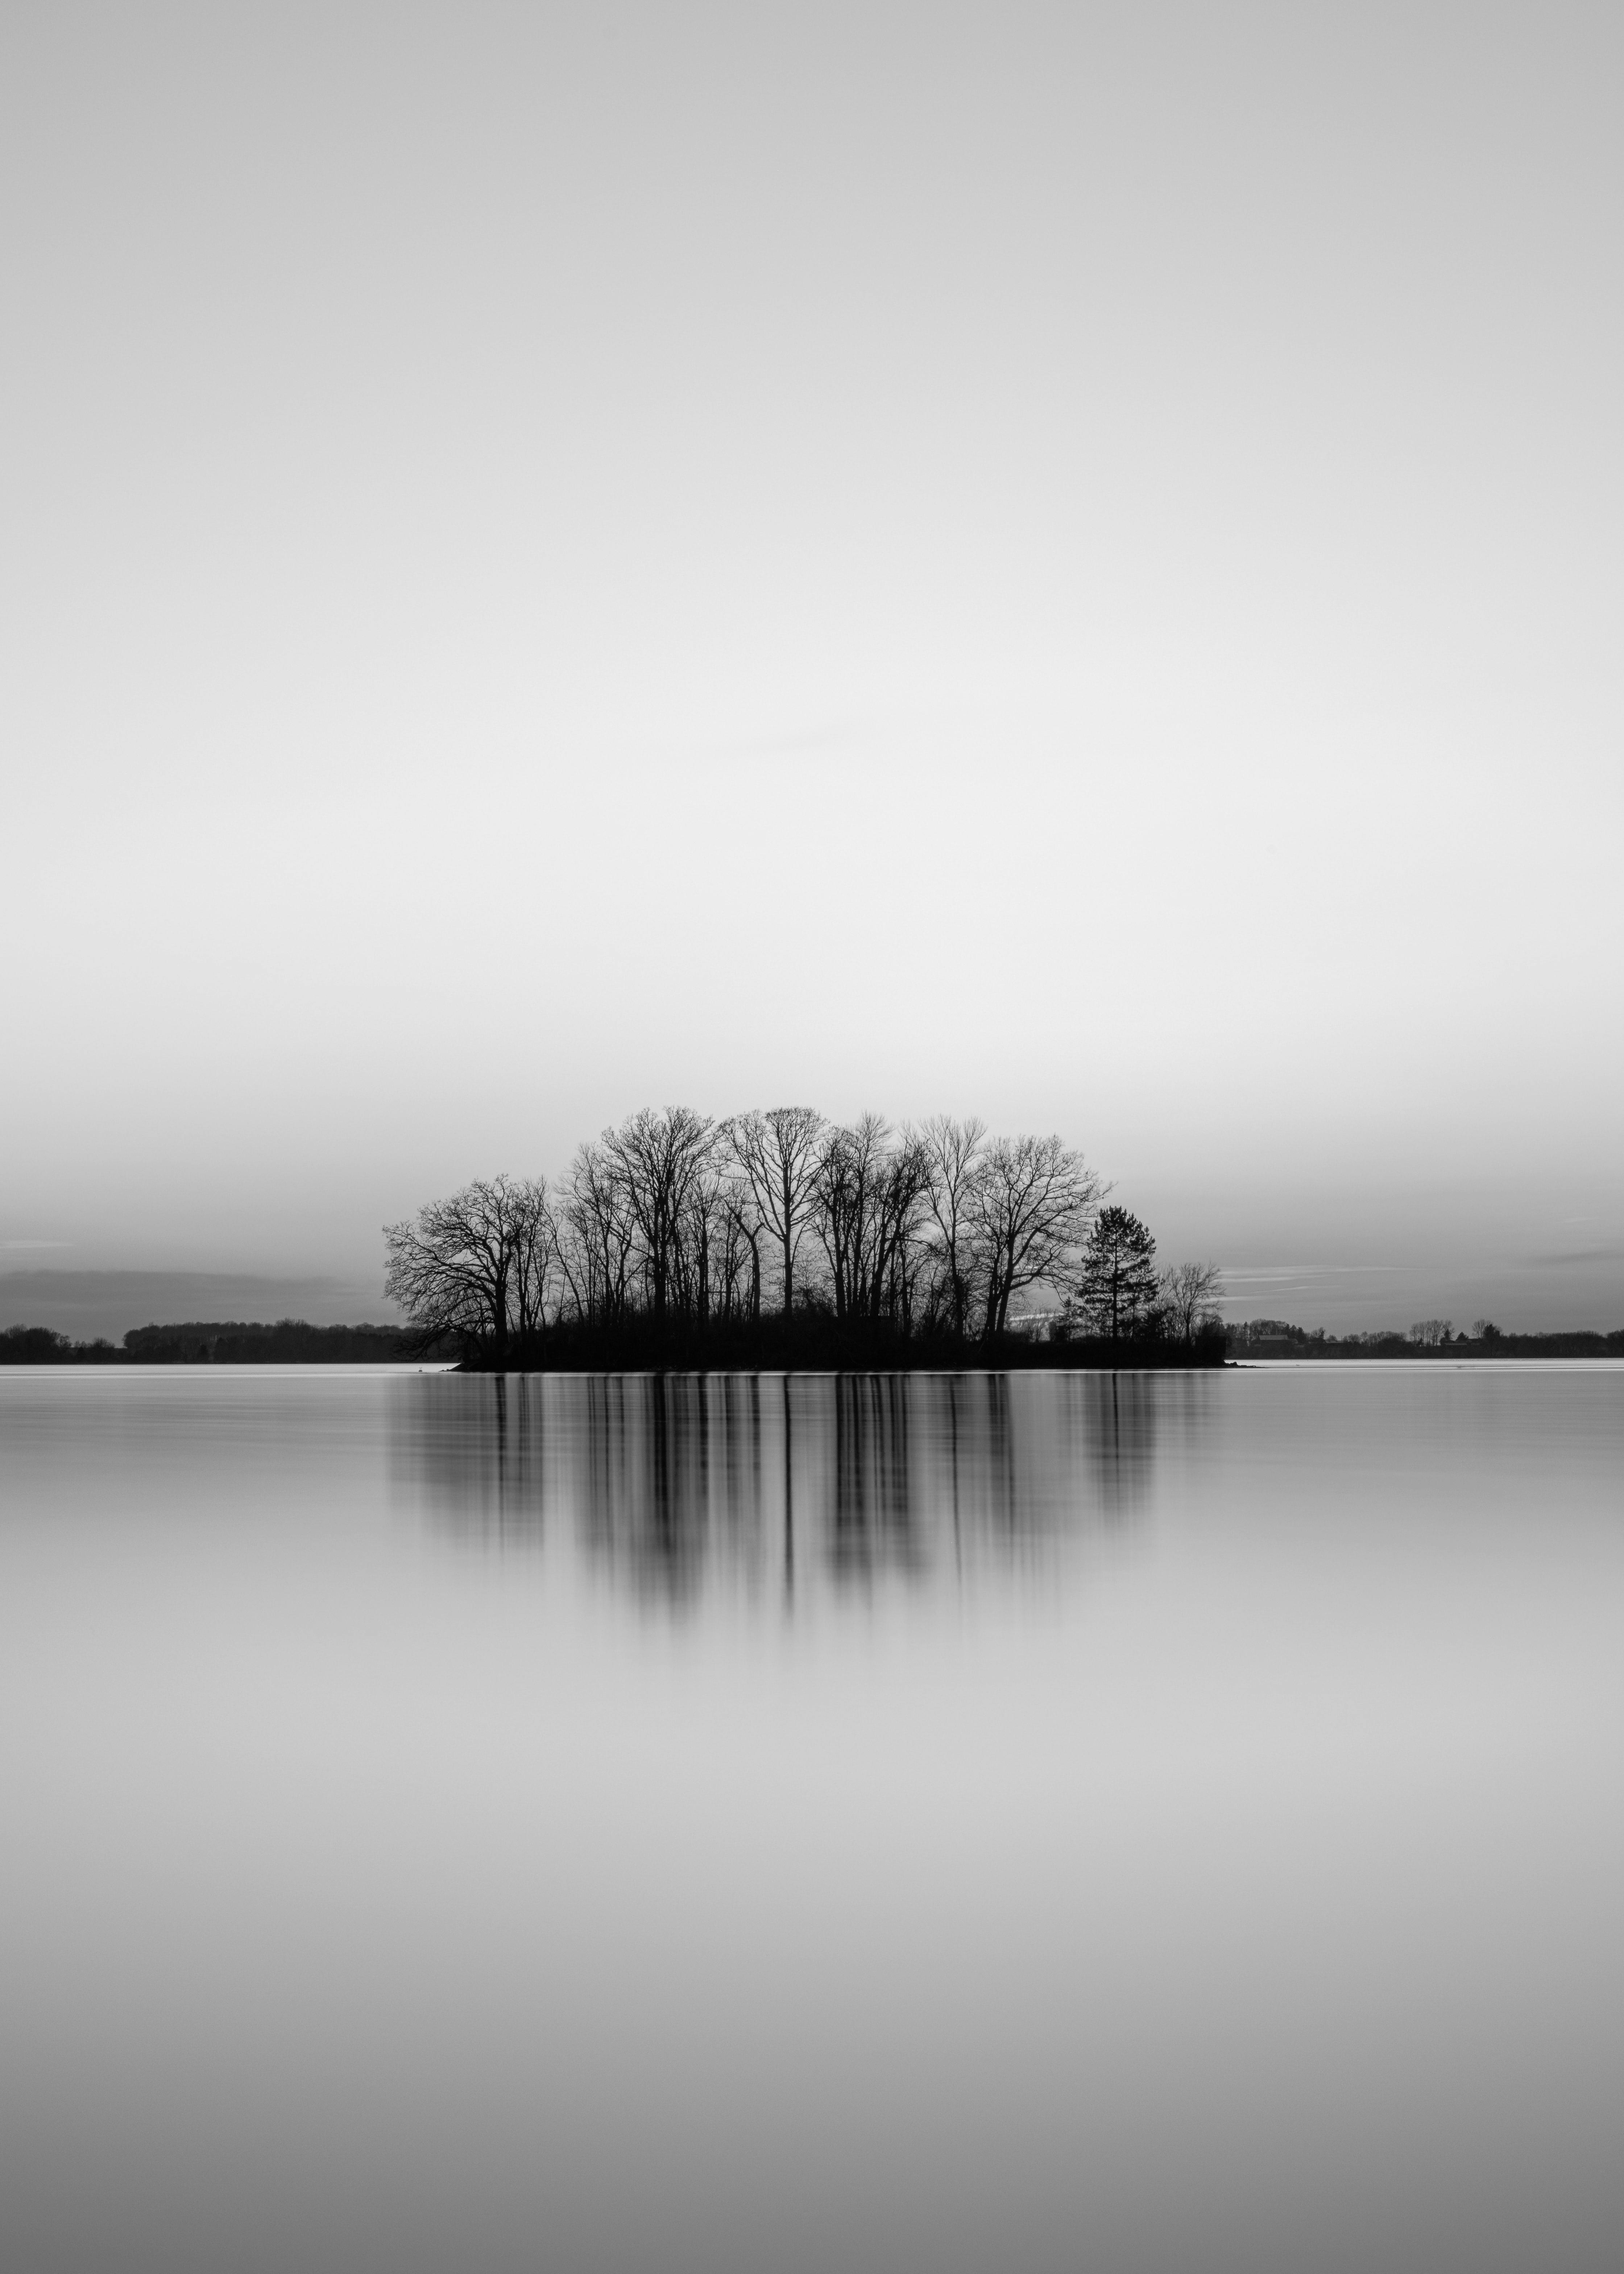
\includegraphics[width=0.33\textwidth]{Assignment-14/fig-1.jpg}
            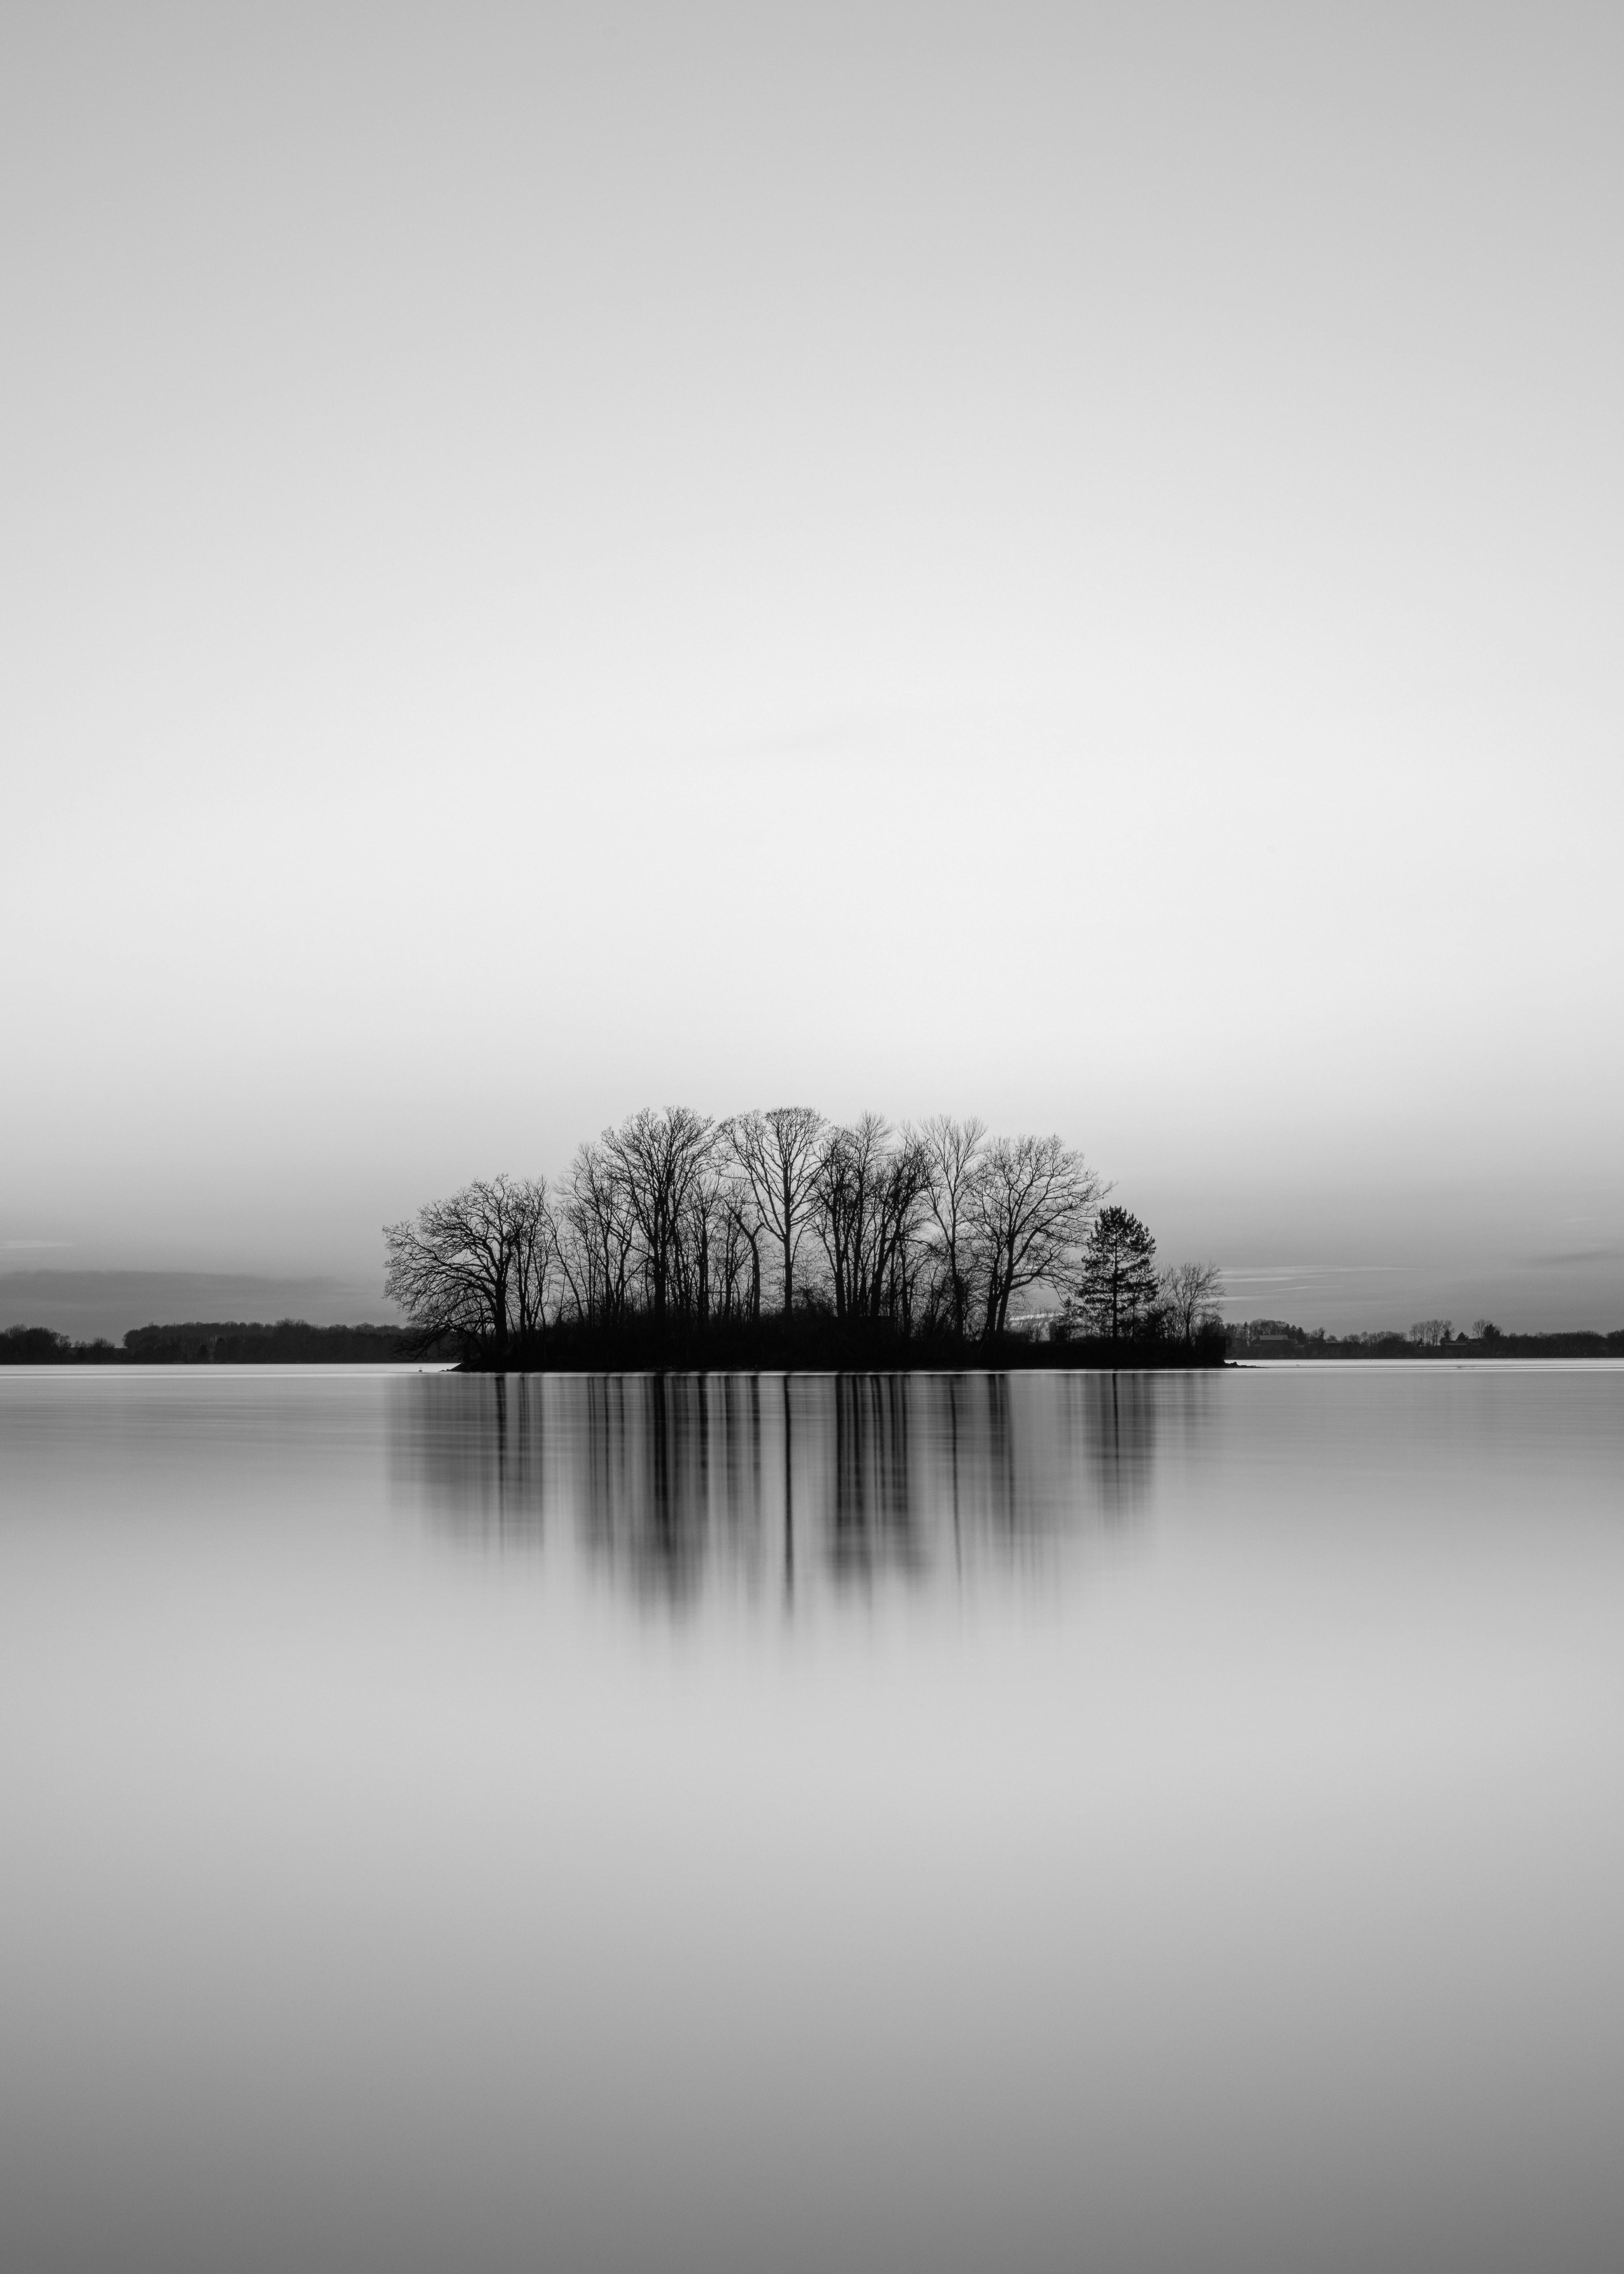
\includegraphics[width=0.33\textwidth]{Assignment-14/fig-2.jpg}
        \end{overprint}
        \begin{overprint}
            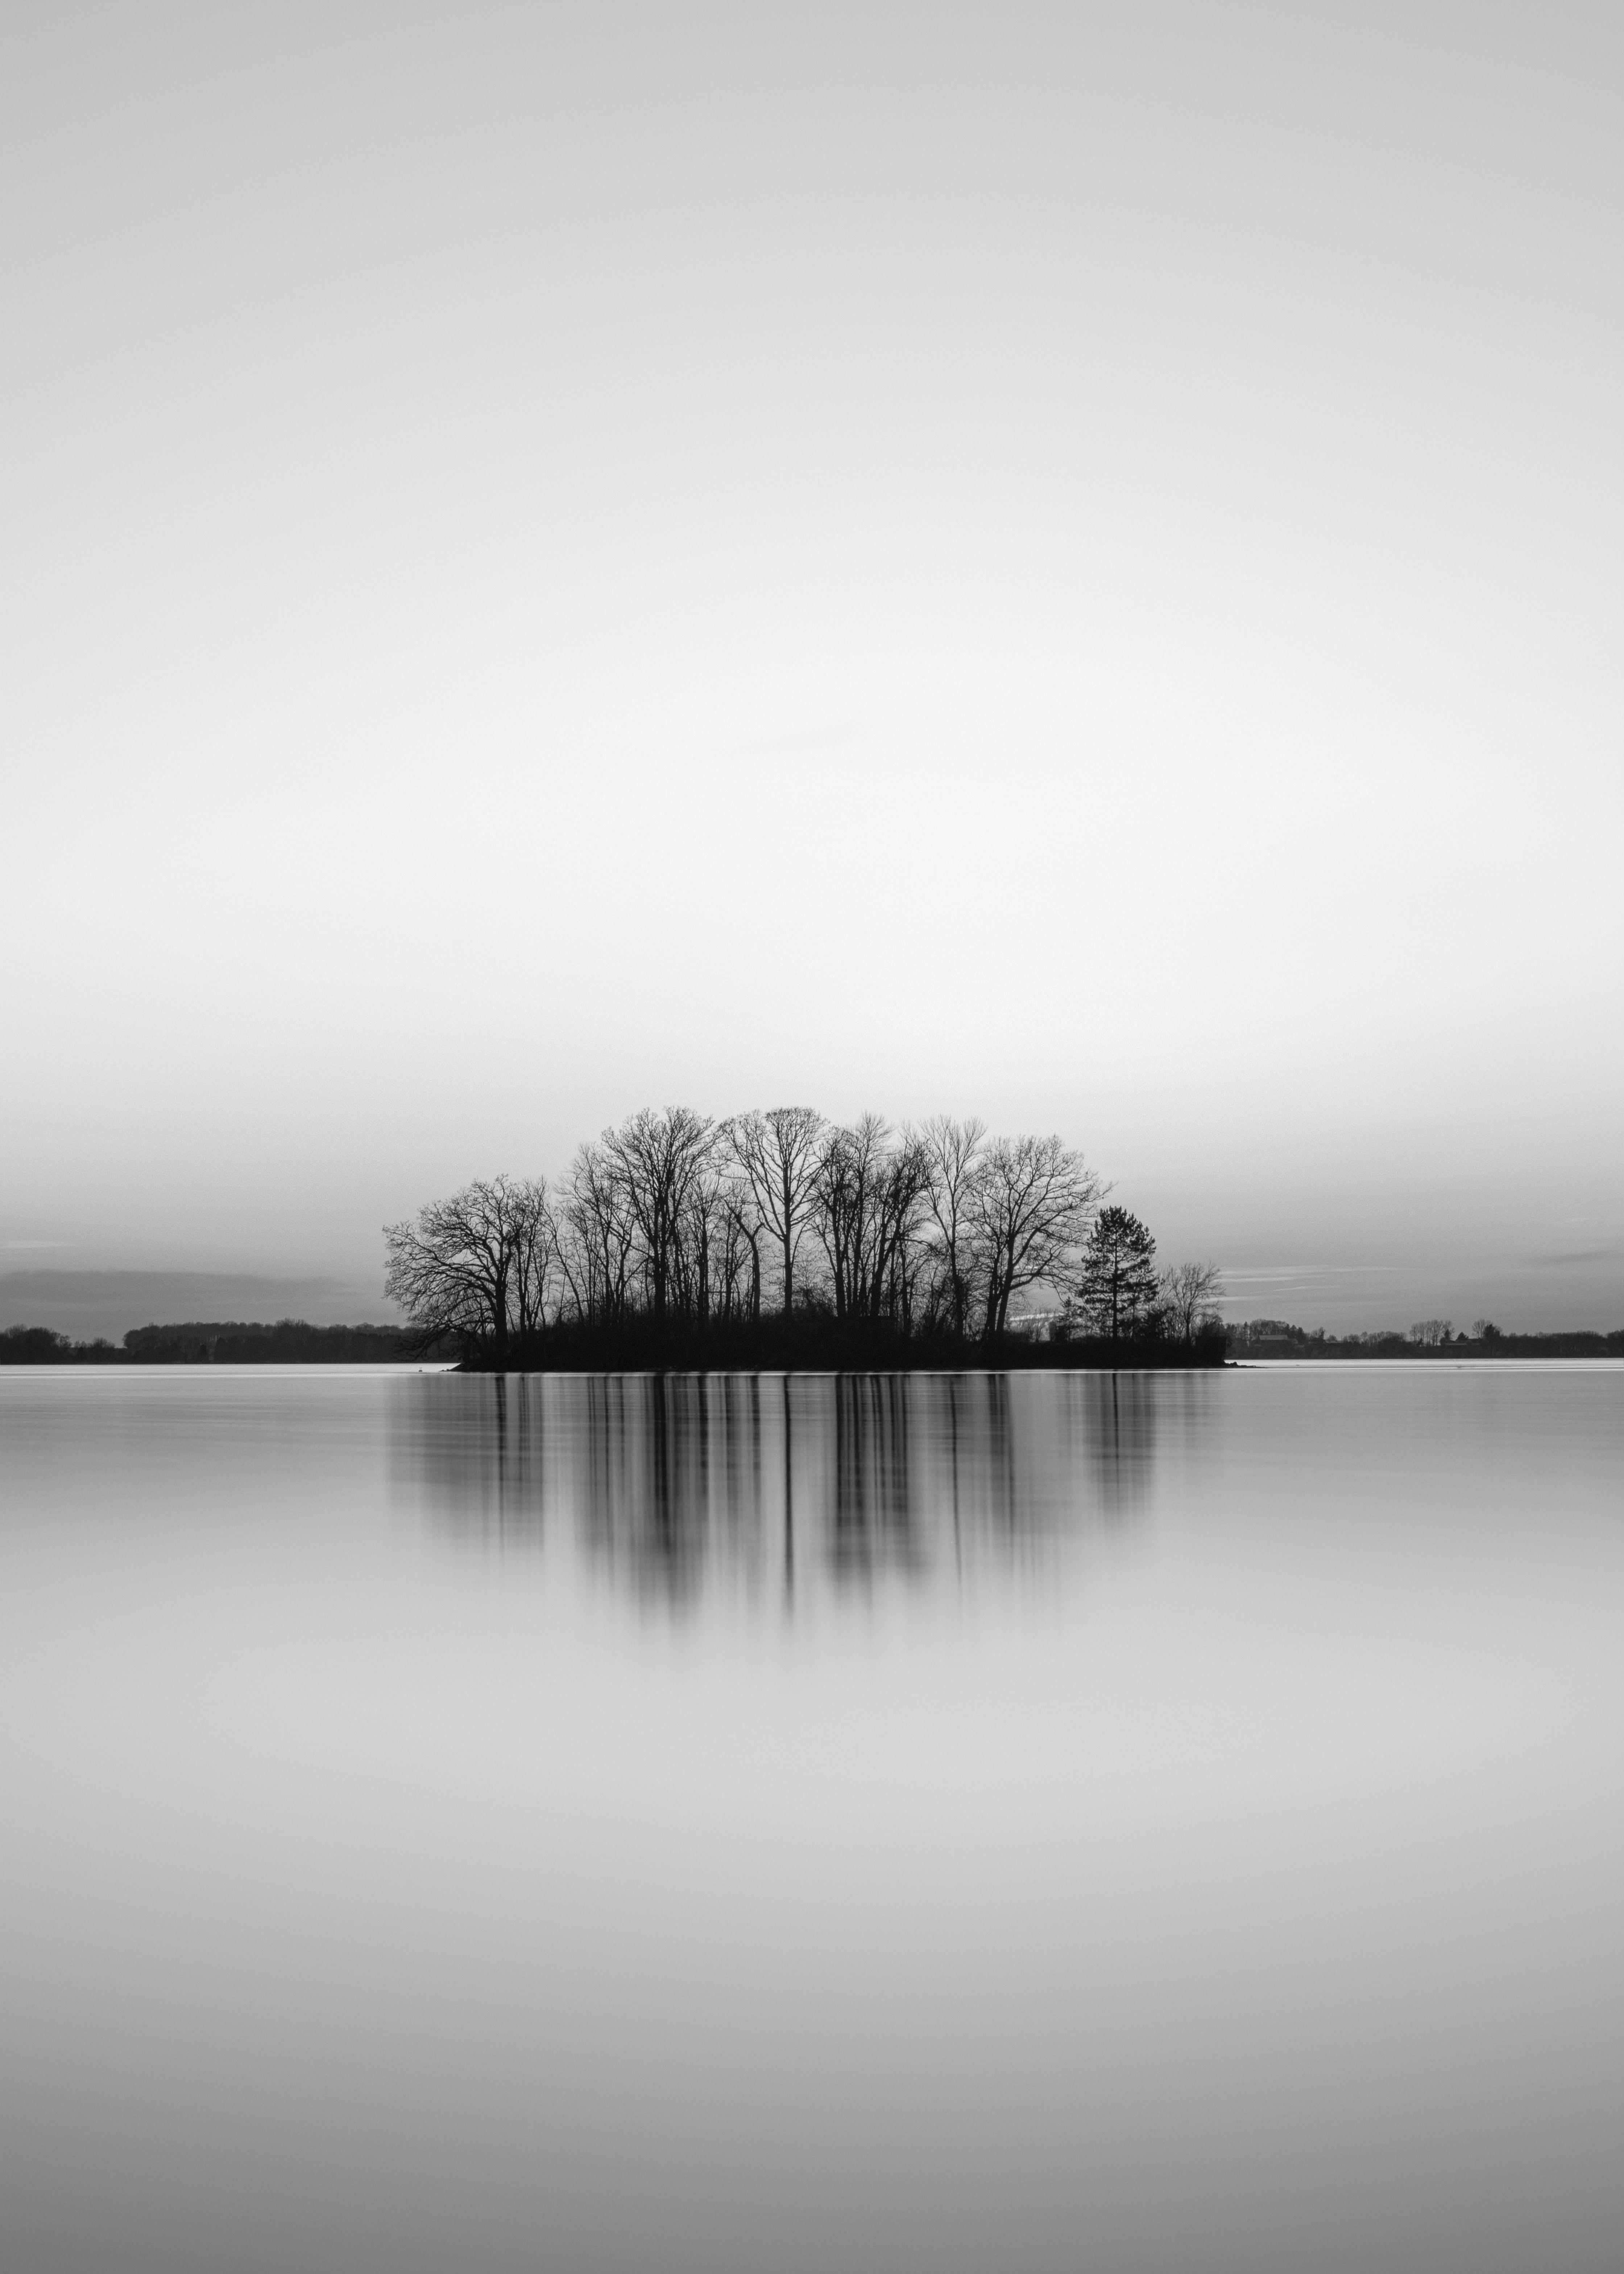
\includegraphics[width=0.33\textwidth]{Assignment-14/fig-3.jpg}
            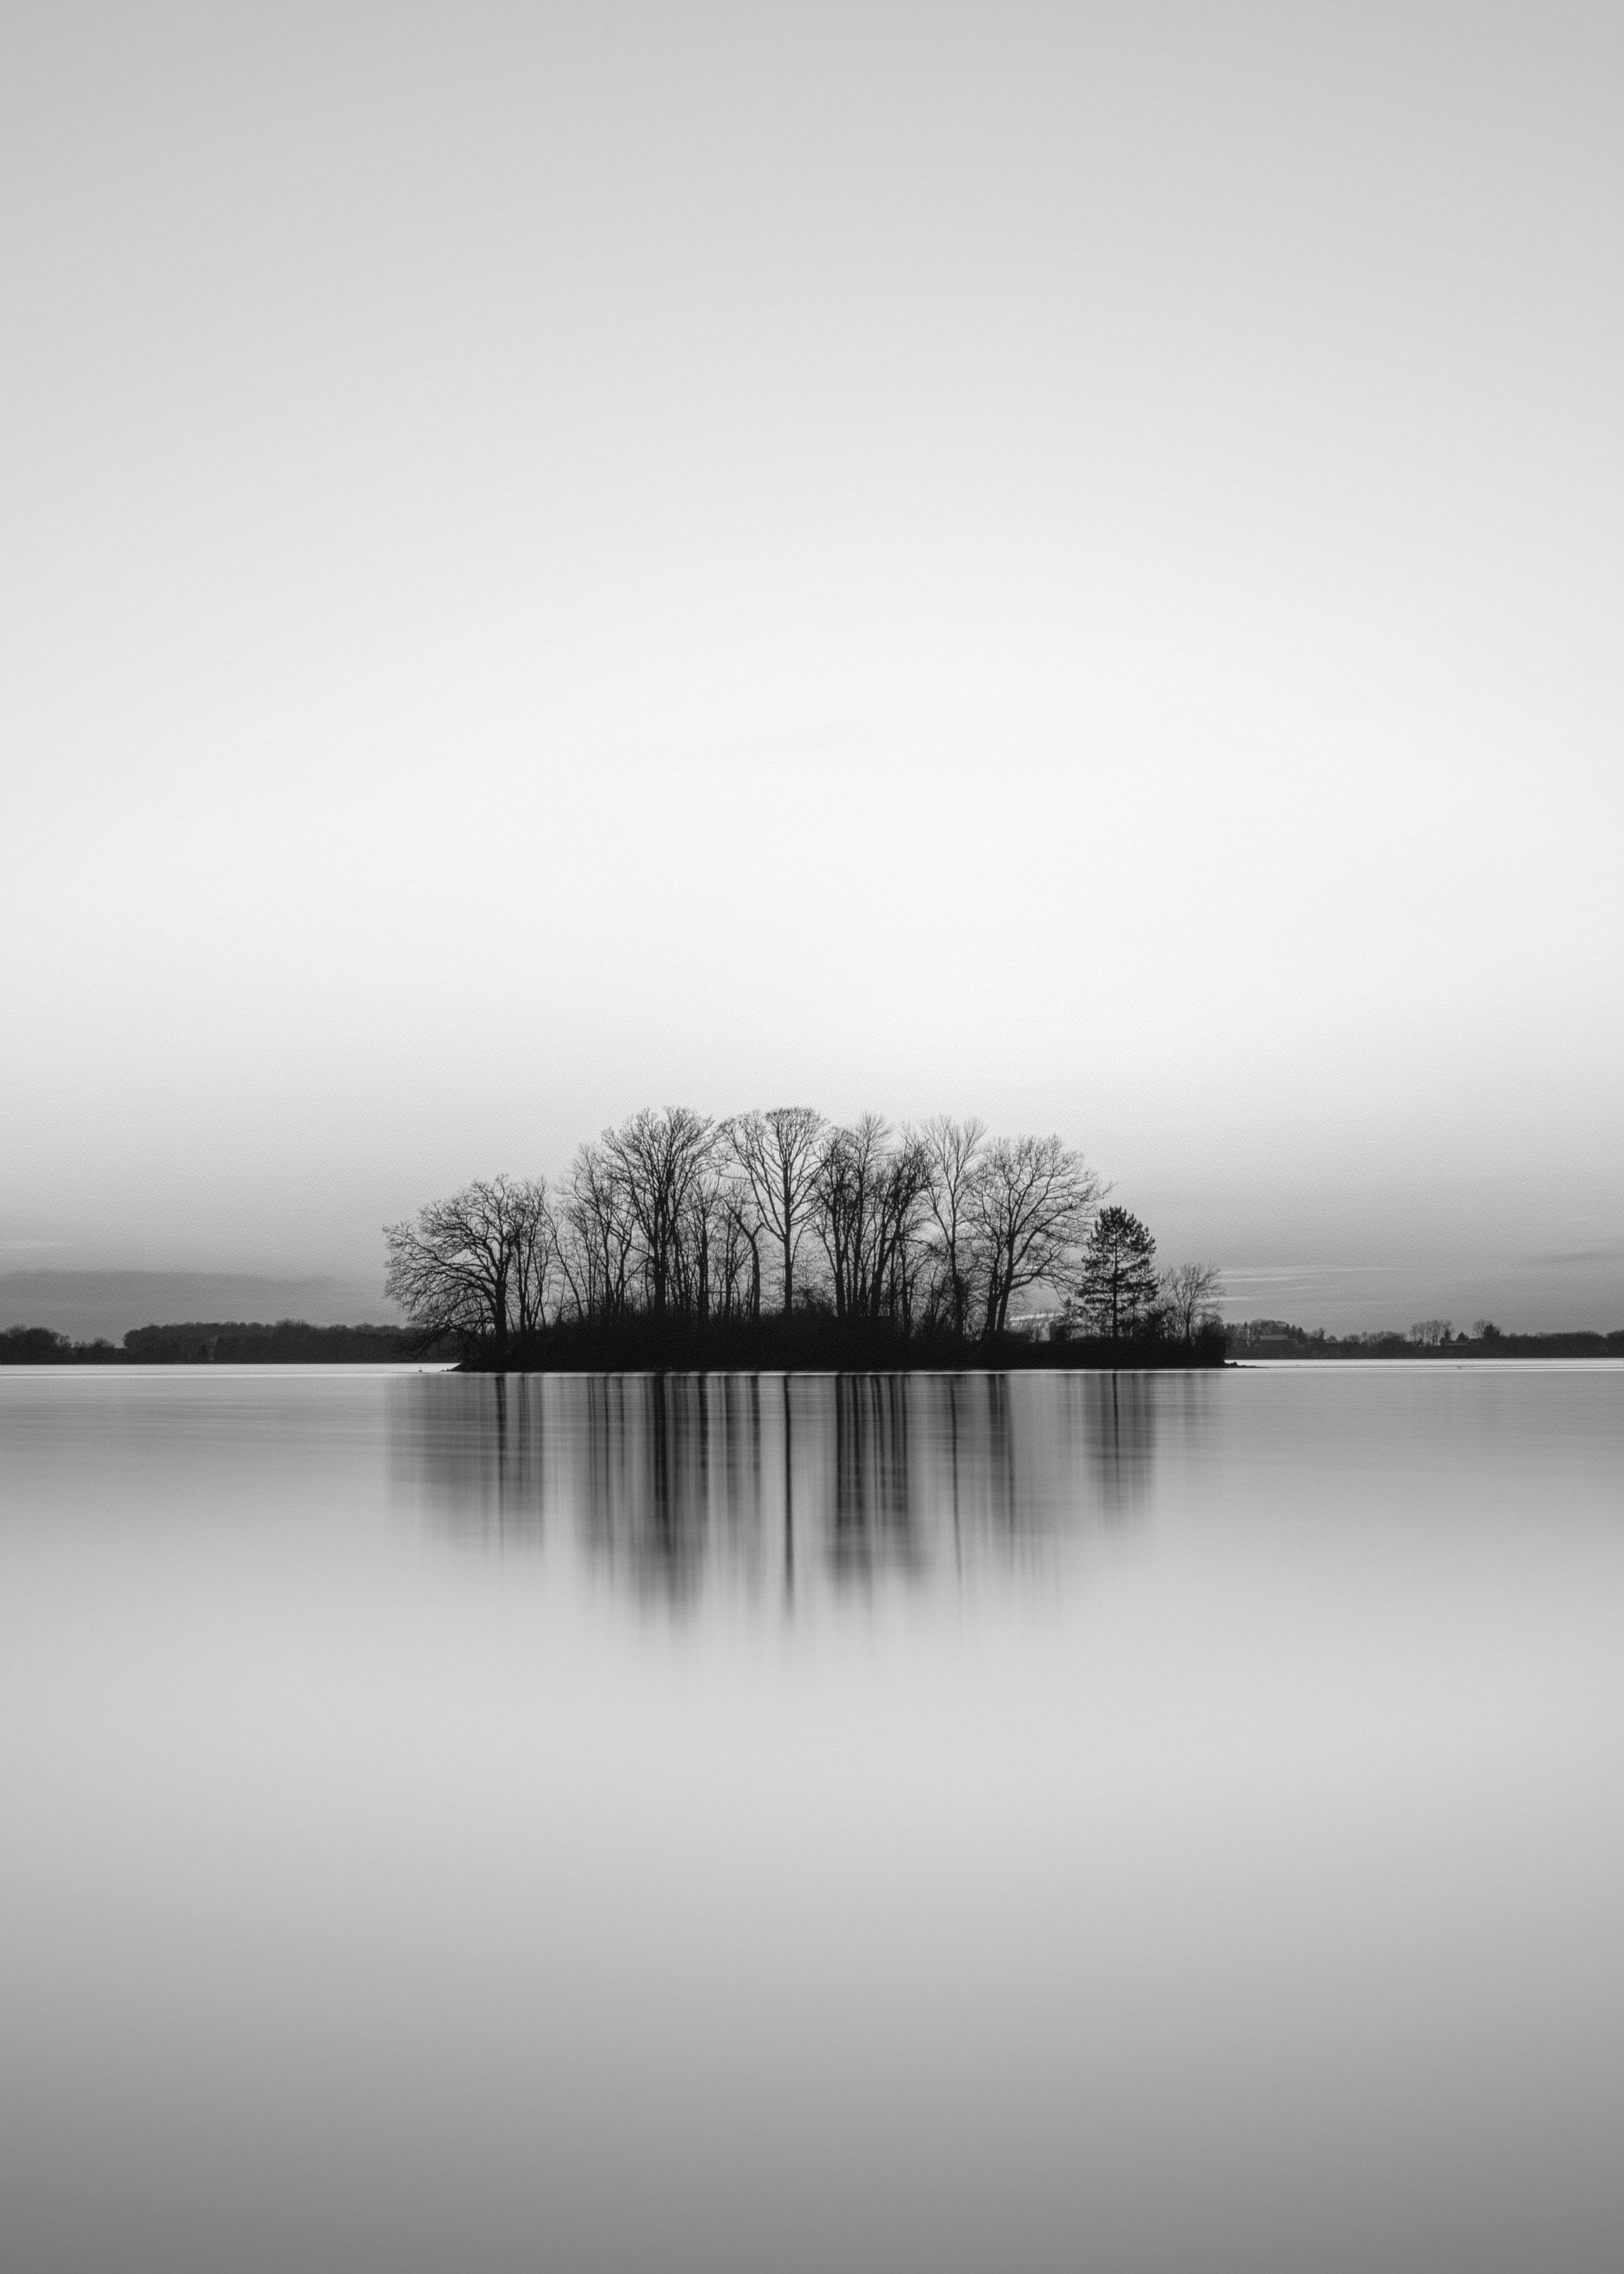
\includegraphics[width=0.33\textwidth]{Assignment-14/fig-4.jpg}
            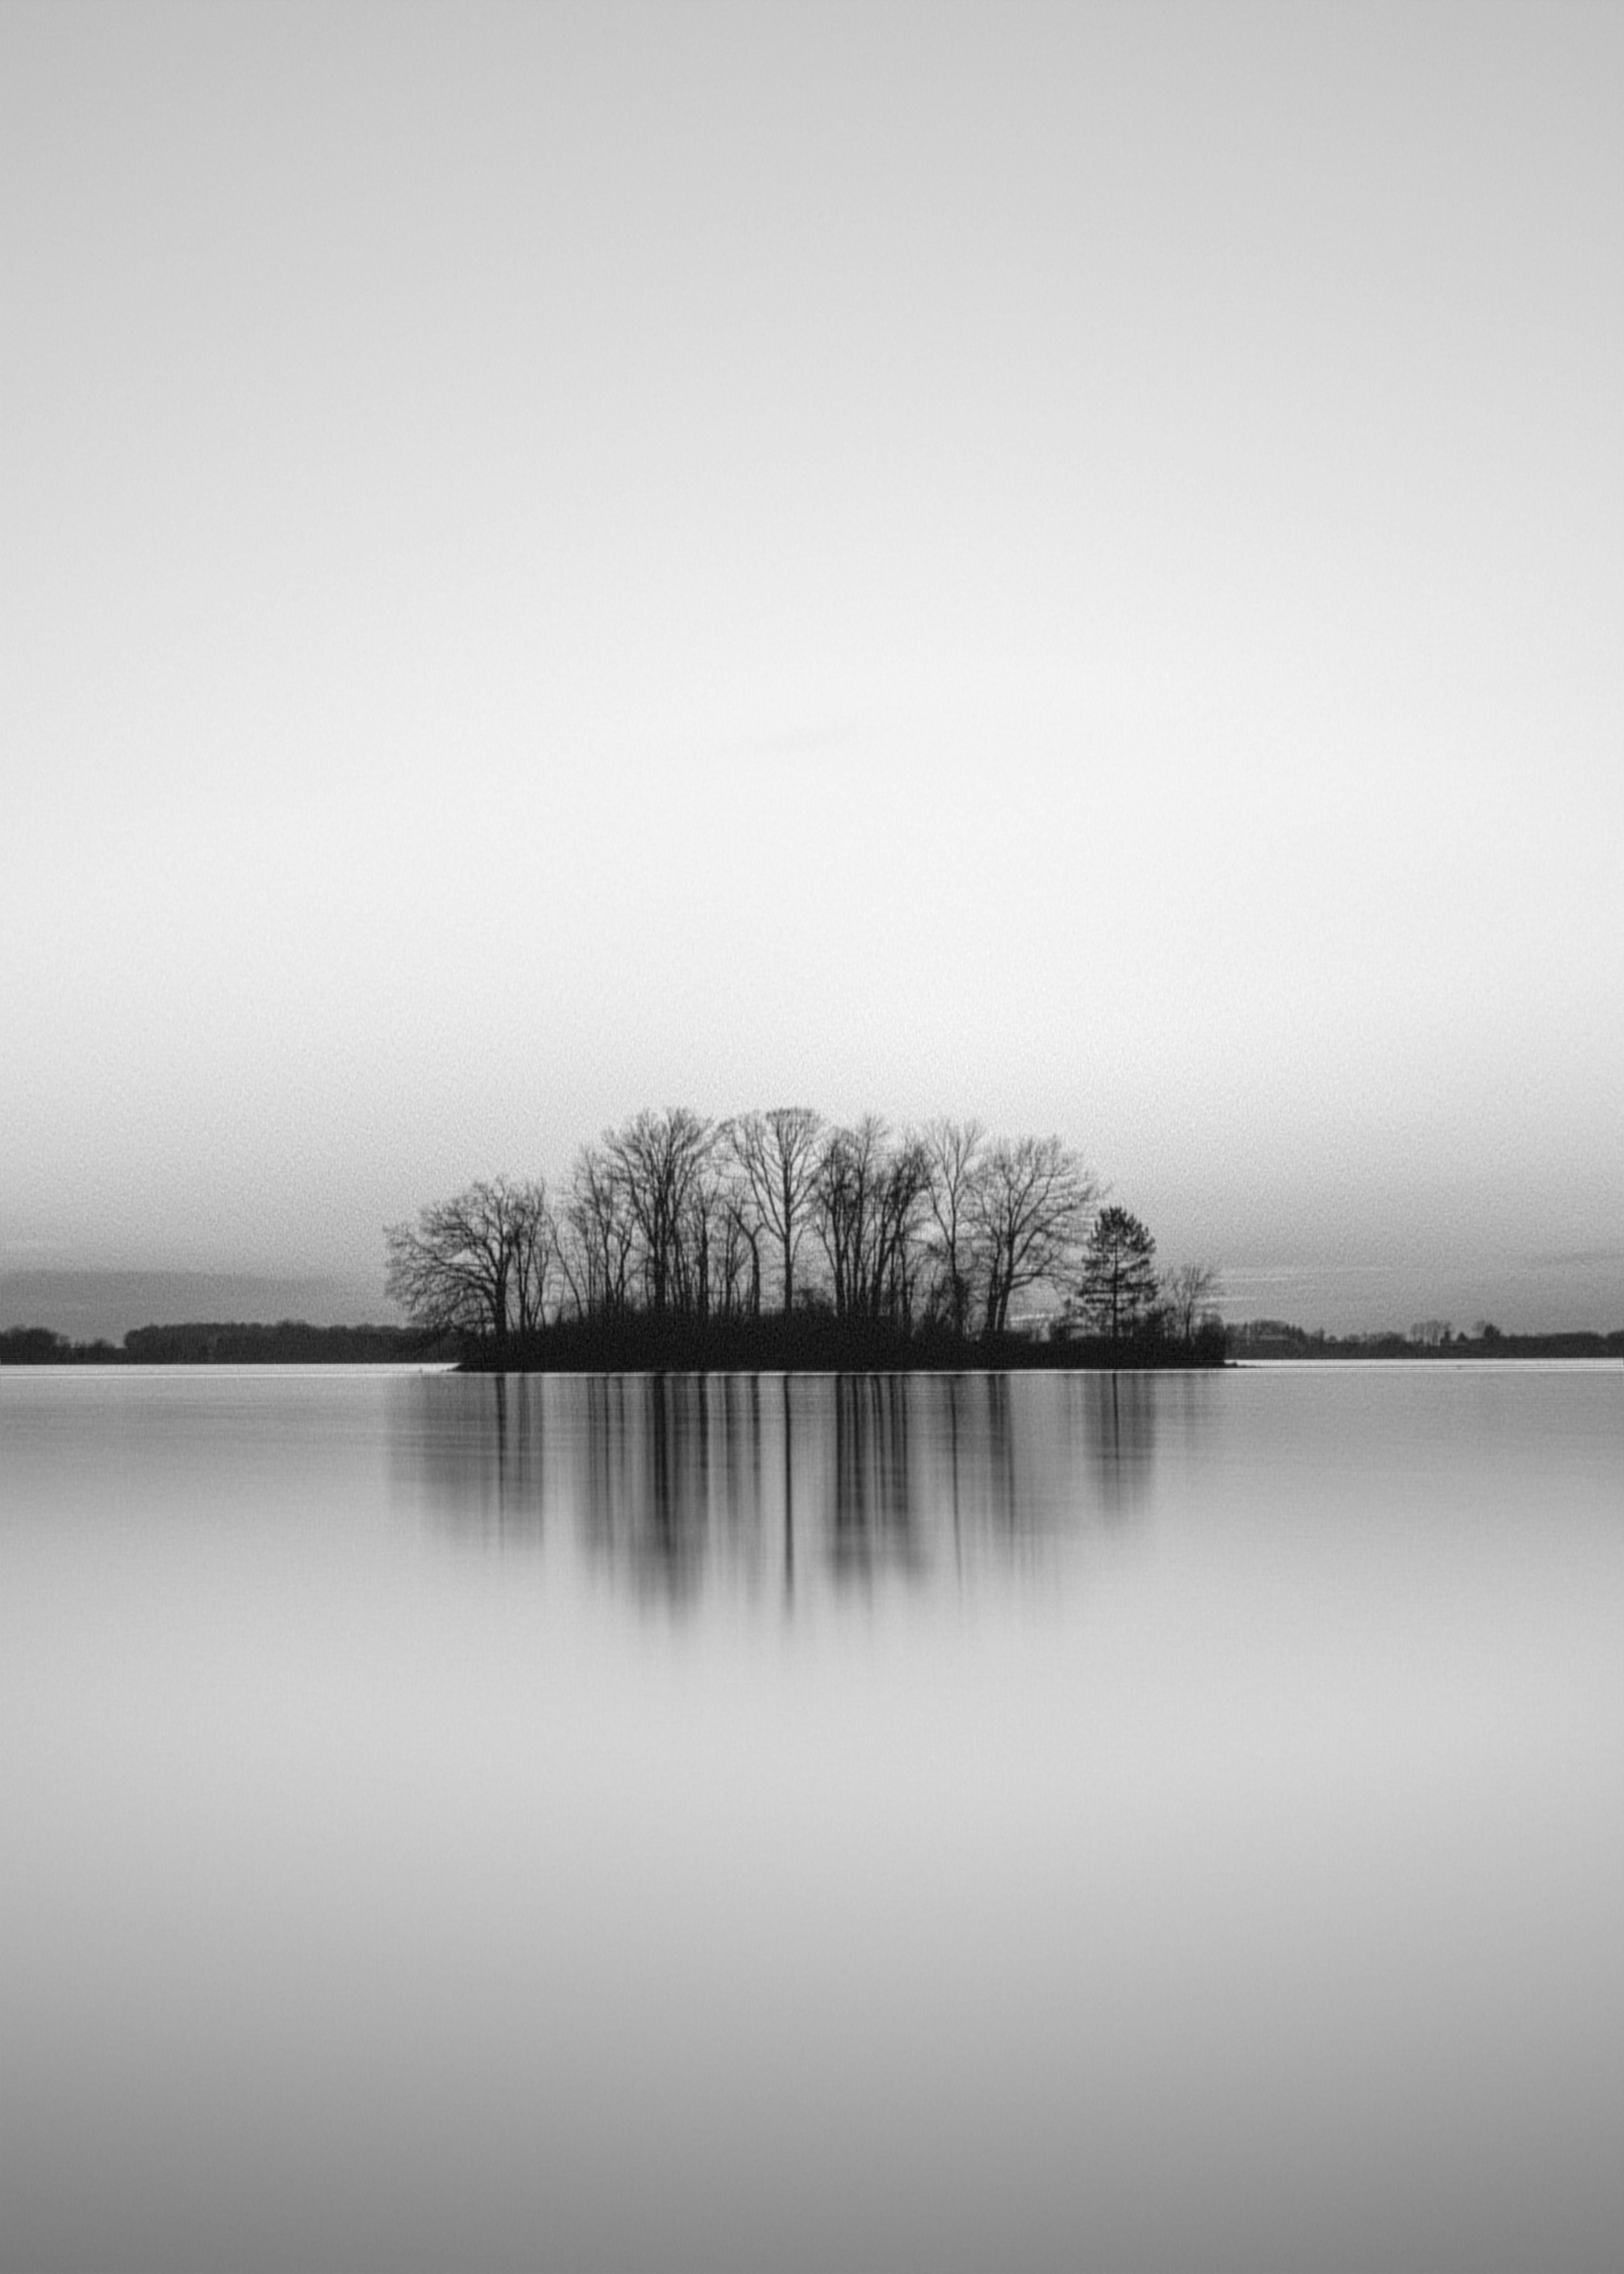
\includegraphics[width=0.33\textwidth]{Assignment-14/fig-5.jpg}
        \end{overprint}
        \begin{overprint}
            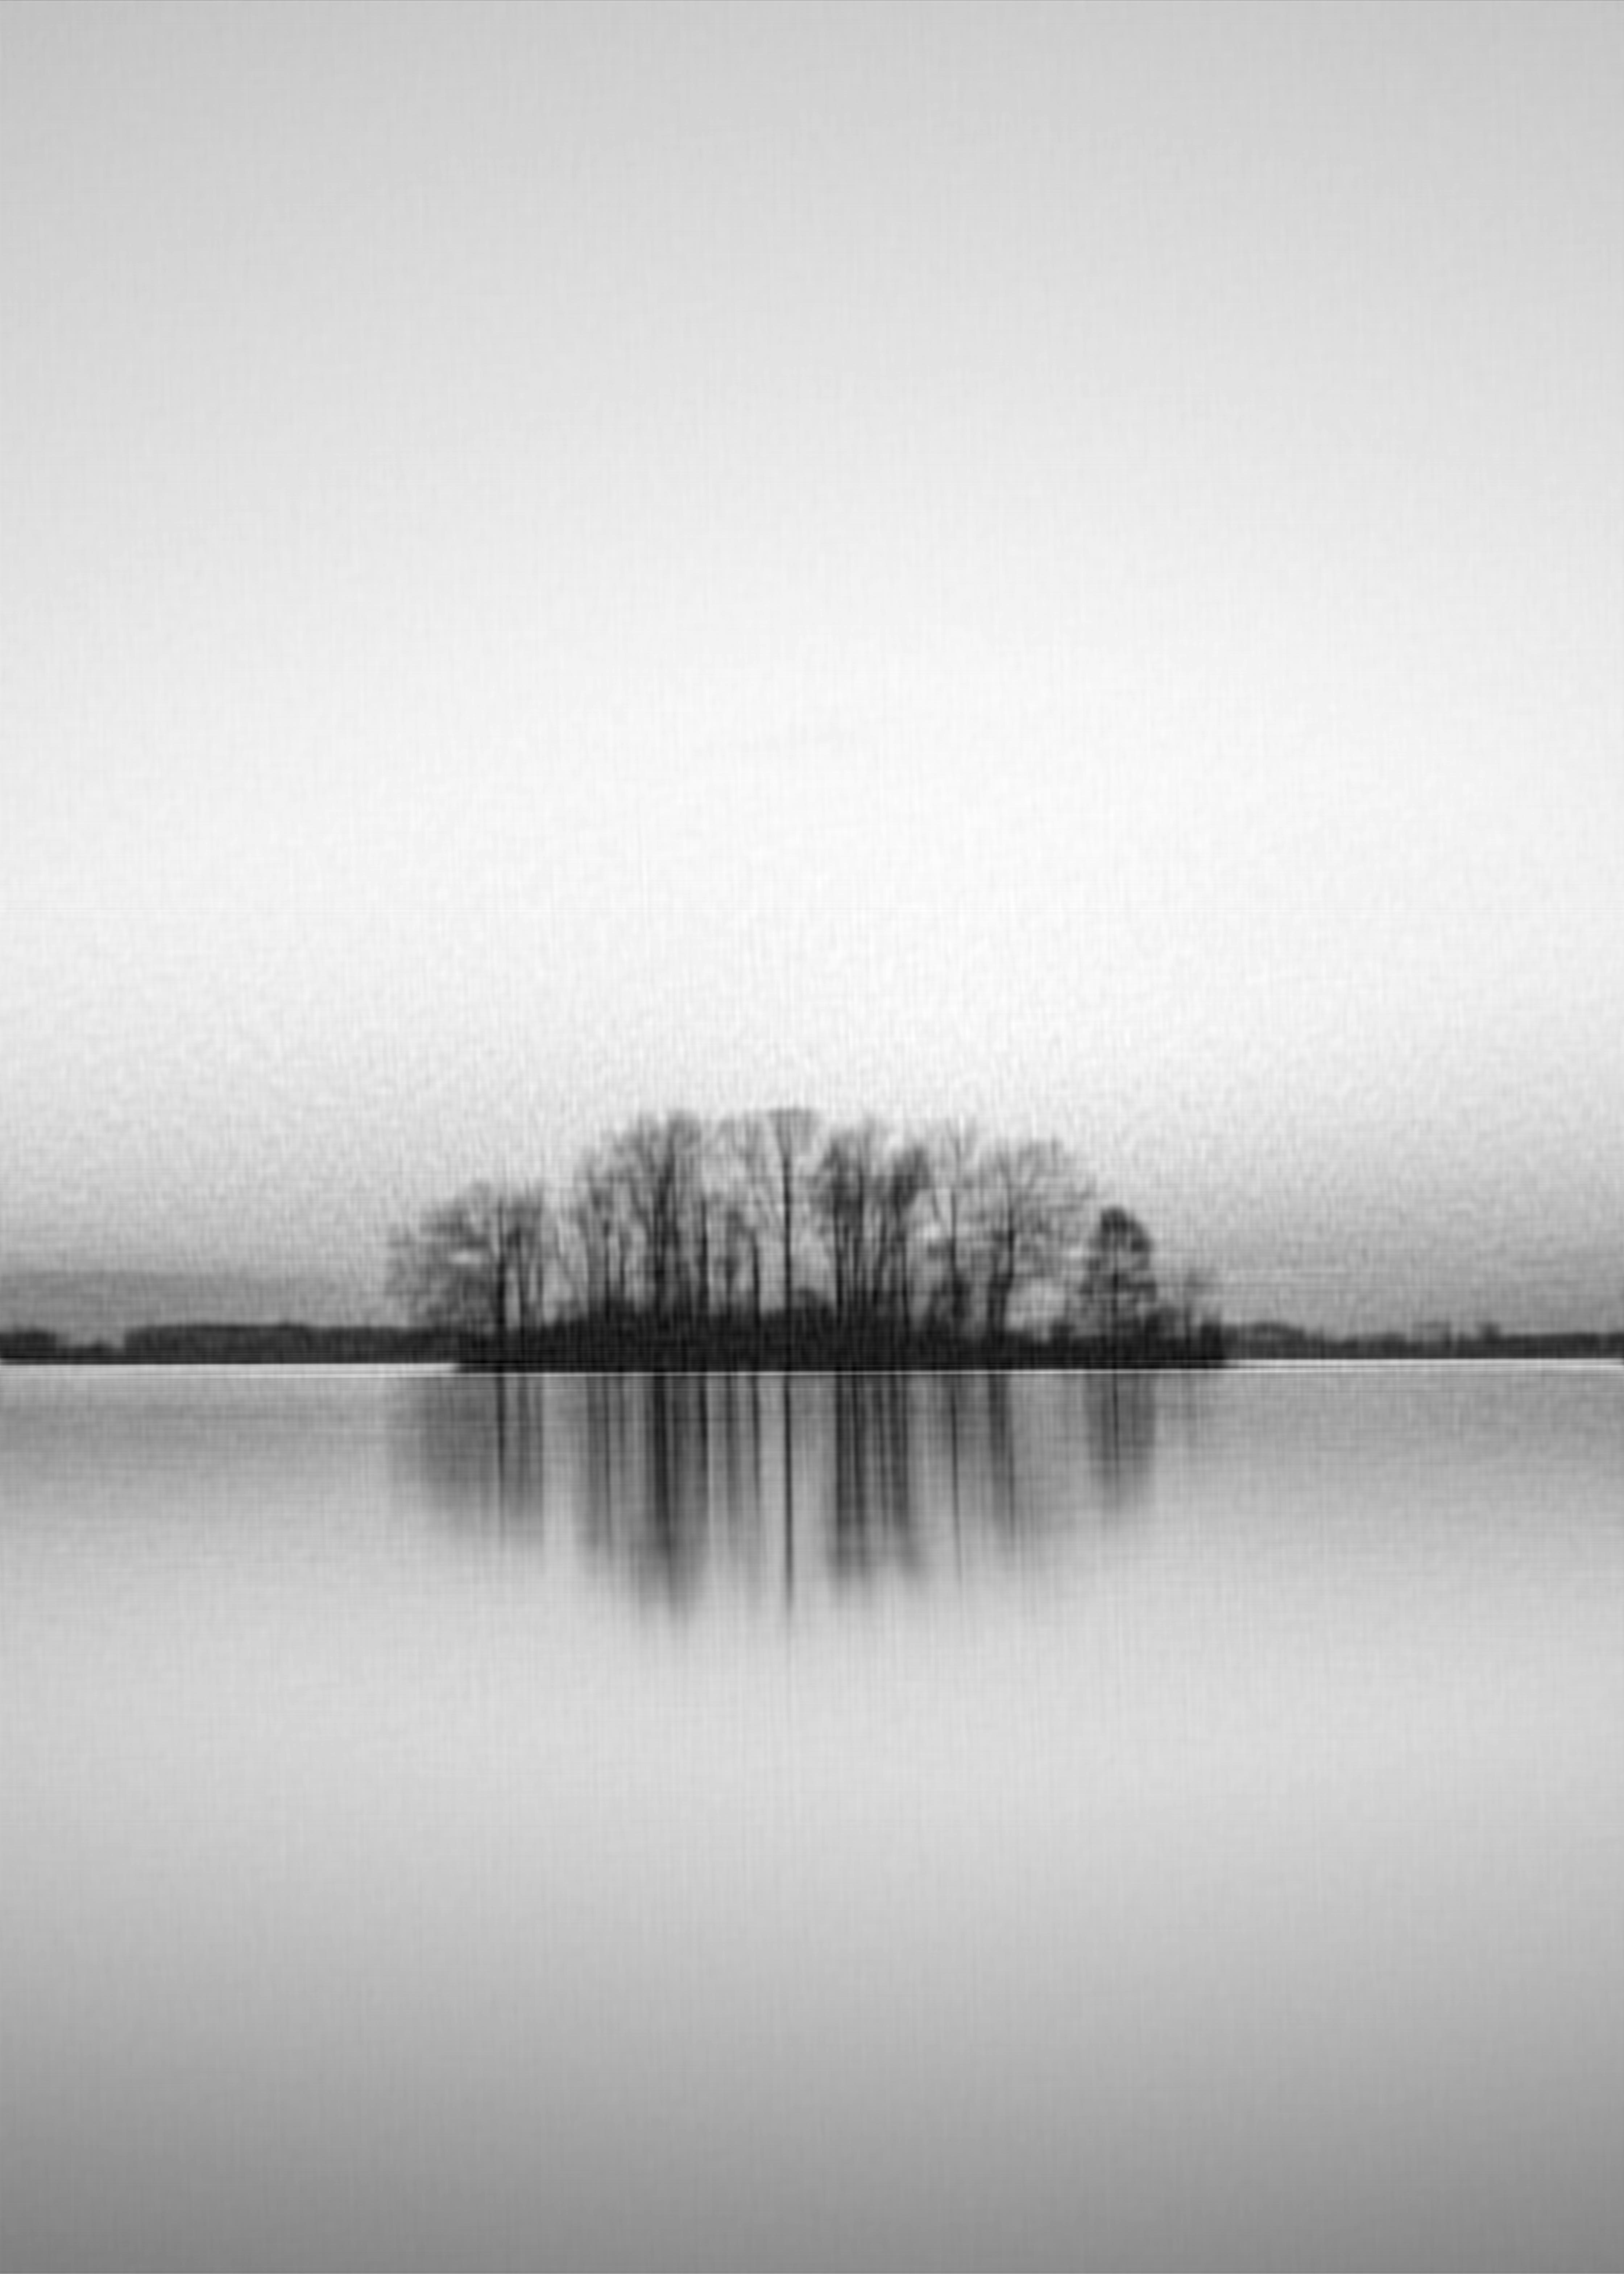
\includegraphics[width=0.33\textwidth]{Assignment-14/fig-6.jpg}
            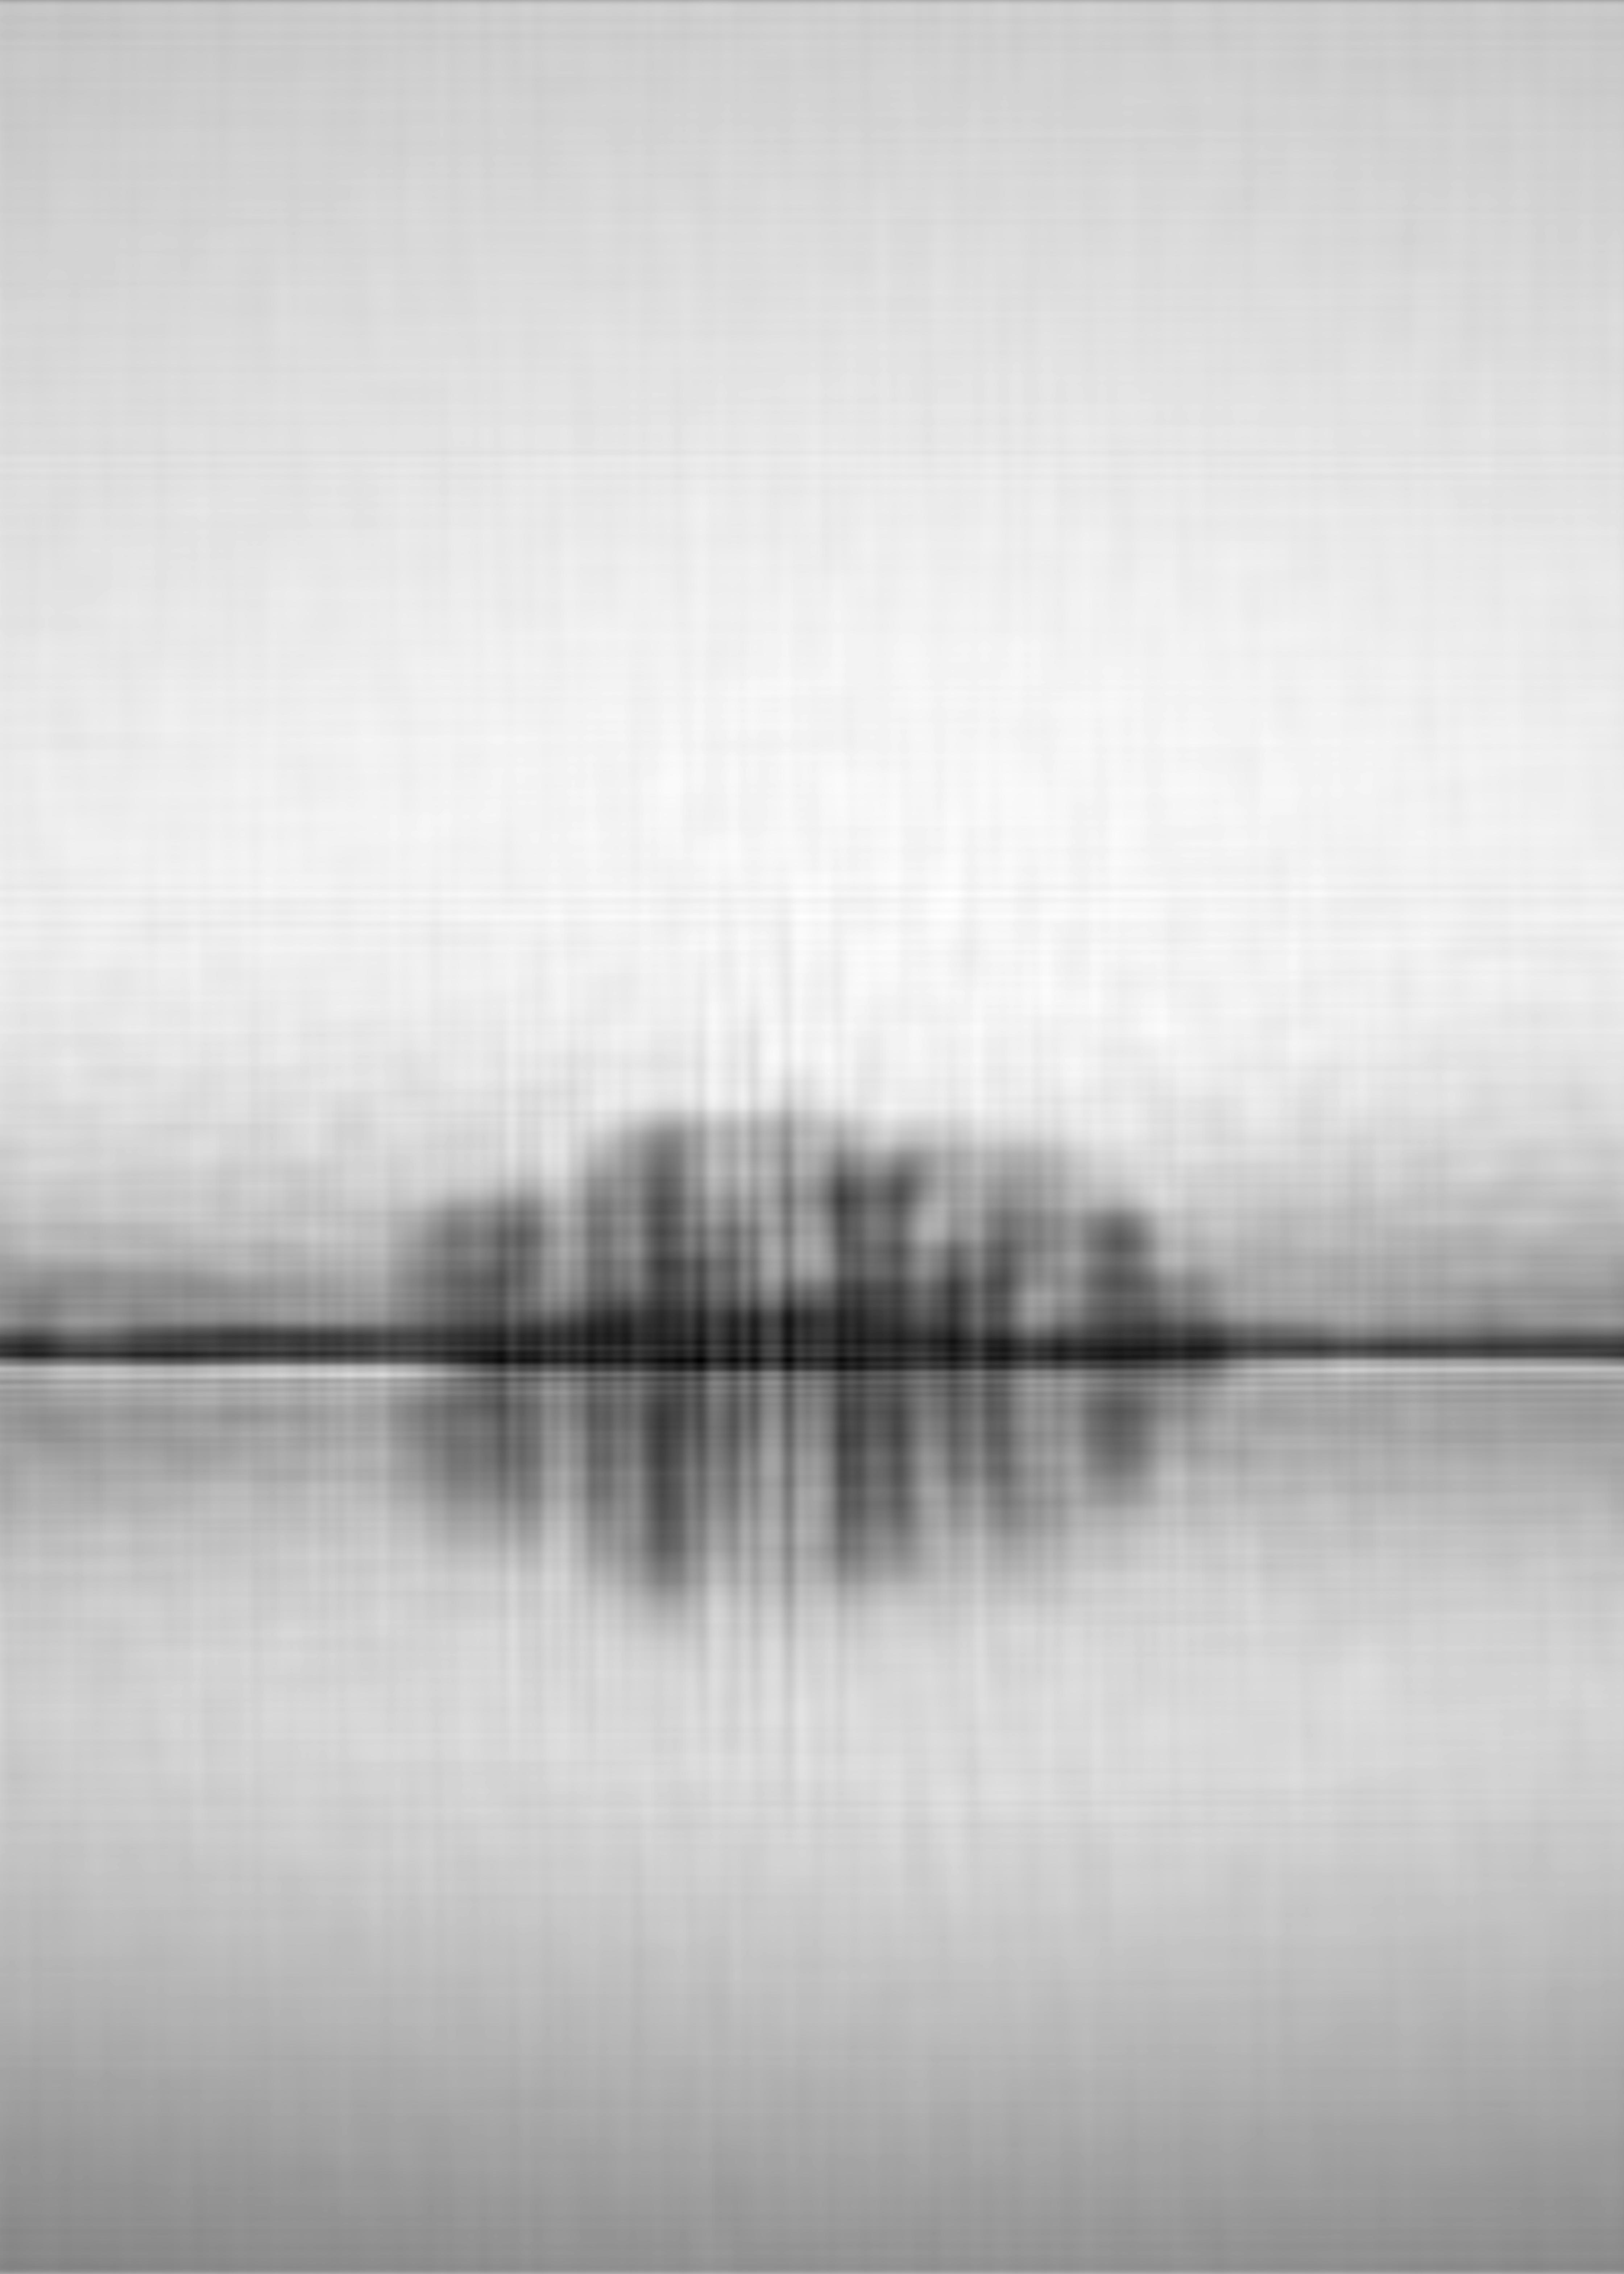
\includegraphics[width=0.33\textwidth]{Assignment-14/fig-7.jpg}
        \end{overprint}
        \caption{Input image of grayscale, output images of compression of 75\%, 50\%, 10\%, 5\%, 1\%, 0.1\%, 0.01\% respectively}
    \end{figure}
}
\clearpage

%-----------------------Assignment-15-------------------------%
{
    \section{Assignment-15}
    \subsection{Introduction}
    \textbf {Problem: }
    Using a smart phone capture both clear and blurry images of a set of objects or scenes. Write a program to deblur those images. Compare neural and non-neural deblurring approaches. You may take help from the provided code to train and test a CNN for deblurring.\\
    \\
    \textbf{Solution: }
    Here at first, we have to blur some images which should be taken through our smartphones. Then with the help of the given model, we have to deblur the images. Obviously all images, here should be in grayscale format. Now for performing this task we have to run the following program.\\
    
    \subsection{Required Software}
    Here we have to install tensorflow which should be installed in a virtual environment. So at fist we have to create a virtual environment then install tensorflow. Again in the virtual environment, we have to install matplotlib, opencv and tk for generating the output. For the first execution of the program, the tensorflow model has to be loaded, so it will take some time to download. After that the program will execute fast.\\
    
    \subsection{Procedure}
    \textbf{Step-1:}
    Install tensorflow, matplotlib, opencv libraries.\\
    \textbf{Step-2:}
    Import the given model in our code.\\
    \textbf{Step-3:}
    Convert the load the RGB images and convert them into grayscale.\\
    \textbf{Step-4:}
    Blur the images using median blur function.\\
    \textbf{Step-5:}
    Deblur the images using the given model.\\
    \textbf{Step-6:}
    Save the output and plot them as required.\\
    
    \subsection{Code}
    \lstset{style=mystyle}
    \begin{lstlisting}[language=Python, caption=Code for blurring and deblurring images]
    import matplotlib.pyplot as plt
    import numpy as np
    import cv2
    import os
    from tensorflow.keras.models import Model, load_model
    
    IMG_SHAPE = (28,28)
    
    def main():    
        model_path = 'Deblurring_CNN.h5'
        model = load_model(model_path)
        
        path = './testdata/'
        testX,testY = prepareTestDataset(path)
    
        output = model.predict(testX)
    
        img_set = [testX[:3, :, :, 0], output[:3, :, :, 0], testY[:3, :, :, 0]]
        title_set = ['Blurred Image', 'Deblurred Image', 'Clear Image']
        plot_img(img_set,title_set)
    
    
    def generate_blurred_img(img_set):
    	n = img_set.shape[0]
    	blurred_img_set = img_set.copy()
    	for i in range(n):
    		blurred_img_set[i] = cv2.medianBlur(img_set[i], 5)
    
    	return blurred_img_set
    
    def prepareTestDataset(path):
        imgs = []
        for file in os.listdir(path):
            img = plt.imread(path+file)
            img = cv2.cvtColor(img,cv2.COLOR_RGB2GRAY)
            img = cv2.resize(img,IMG_SHAPE)
            imgs.append(img)
        
        testY = np.array(imgs)
        testX = generate_blurred_img(testY)
        testY = np.expand_dims(testY,axis=3)
        testX = np.expand_dims(testX,axis=3)
        print("testX shape: ",testX.shape)
        return testX,testY
    
    def plot_img(img_set, title_set):
    	plt.figure(figsize = (20, 20))
    	# plt.rcParams['font.size'] = 4
    	n = len(img_set)
    	k = 1
    	for i in range(n):
    		for j in range(3):
    			plt.subplot(n, 3, k)
    			plt.imshow(img_set[i][j], cmap = 'gray')
    			plt.axis('off')
    			plt.title(title_set[i])
    			k += 1
    
    	plt.savefig('fig-1.jpg')
    	plt.show()
    
    if __name__ == '__main__':
        main()

    \end{lstlisting}
    \\
    \subsection{Result & Discussion}{
        Here the training data is saved in 'testdata' folder which we trained for testing after making them blurred using the median blur function and then main images becomes the test data. We reshape the images for fast computing. Now the output of the deblur image is shown below. From there we can see that the deblurring operation does not perform so good. Only for bright picture, some information is restored. Otherwise, it is not so effective. If we want to improve our accuracy, we have to create our personal dataset for training and testing.
        
        \begin{figure}[htp]
            
            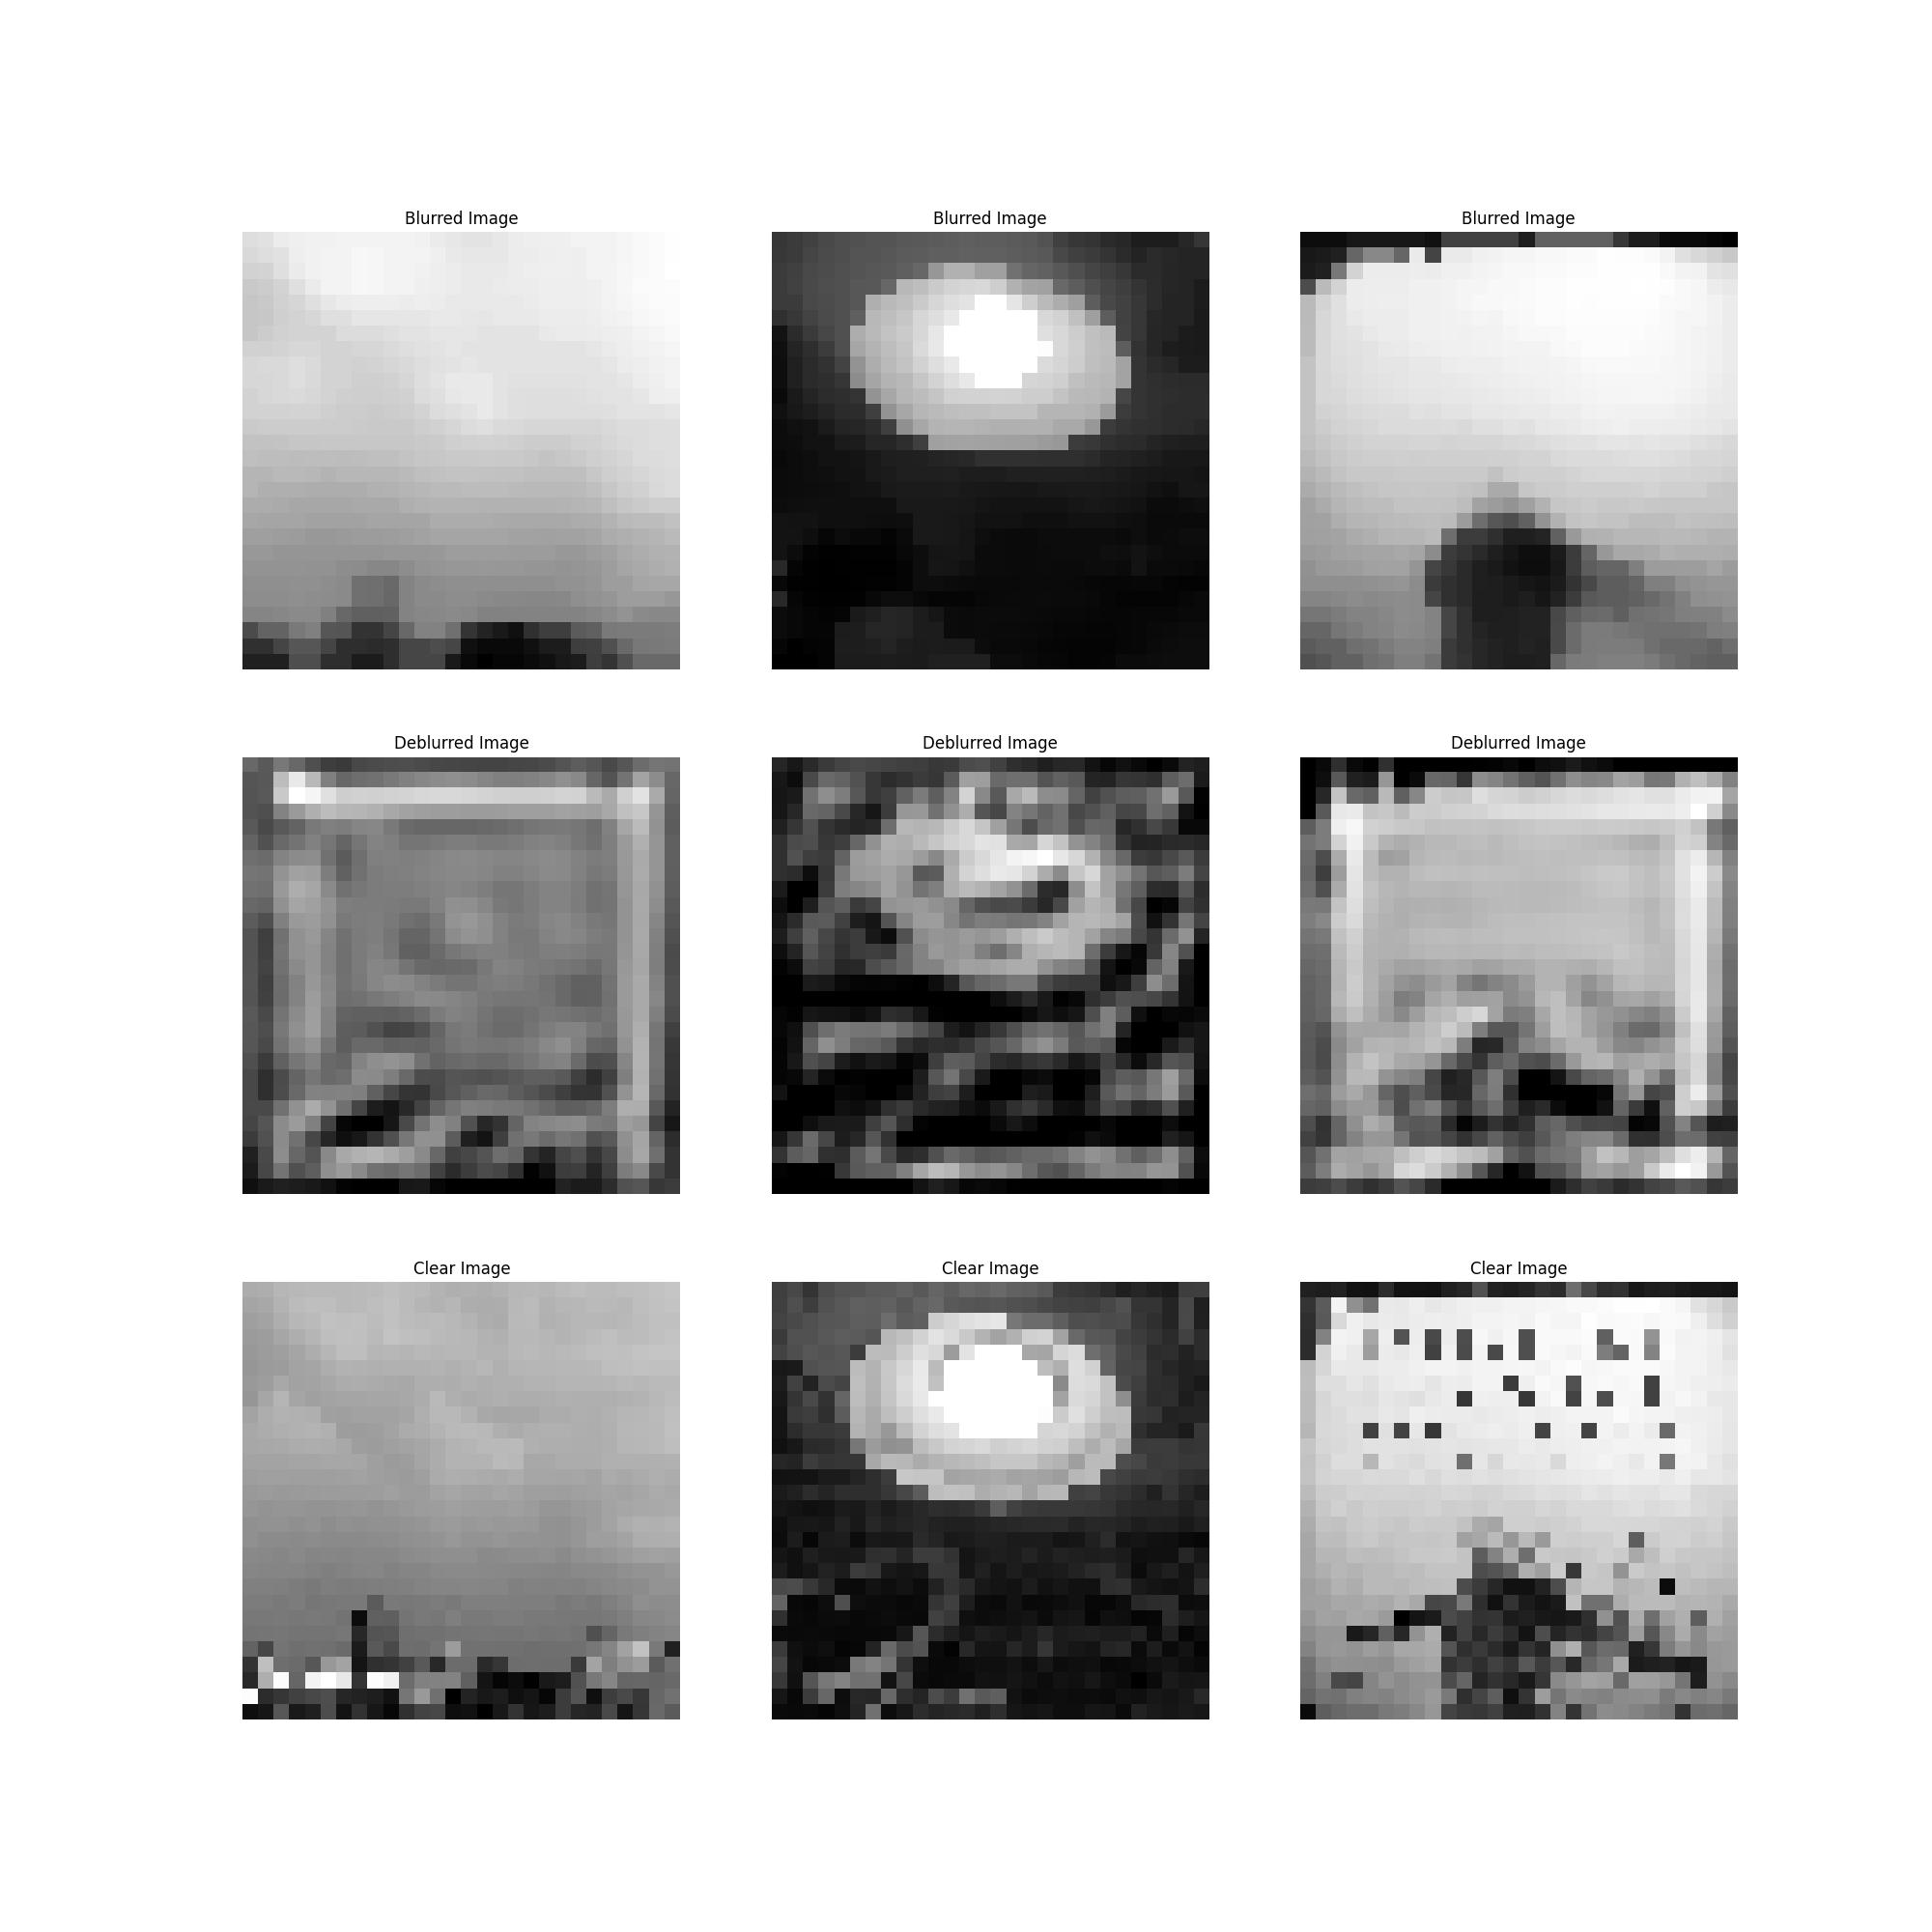
\includegraphics[width=1.0\textwidth]{Assignment-15/fig-1.jpg}
            \caption{Output of deblurring operation}
        \end{figure}
    }
}
% \pagebreak
\clearpage

\end{document}